%%%%%%%%%%%%%%%%%%%% UG4A %%%%%%
\documentclass[graybox,envcountchap,sectrefs,UStrade]{svmono}
% adopted svmono class file [http://www.springer.com/authors/book+authors?SGWID=0-154102-12-417900-0]

\usepackage{amsmath,amssymb,textcomp}
\usepackage[T1]{fontenc}
\usepackage{mathptmx}
\usepackage{verbatim}
\usepackage{helvet}
\usepackage{booktabs}
\usepackage{courier}
\usepackage{array,tabularx,multirow,rotating} %Table format packages
\usepackage{natbib} %Format for references
\usepackage{textcomp,eurosym}
\usepackage{wrapfig}
\usepackage[switch,pagewise]{lineno}
\usepackage{fancyhdr,fancybox}
\usepackage{url}
\usepackage{hyperref}            %automatic hyperlinks in document; redefines
\hypersetup{colorlinks=true, linkcolor=black, citecolor=black,
        urlcolor=black, bookmarks=true, bookmarksnumbered=true,
        bookmarksopen=true, pdfview=FitH, pdfstartview=FitH,
        pdftitle={The Unofficial Guide for Authors},
        pdfauthor={Tomislav Hengl, Michael Gould and Wouter Gerritsma},}

% Margin paragraphs:
\setlength{\marginparwidth}{1.8cm}
\setlength{\marginparsep}{4pt}

%% Fix page layout:
\usepackage[top=1.6cm, bottom=2cm, left=2.1cm, right=2.1cm]{geometry}
% fix the font size and encoding for url's etc:
\renewcommand{\ttdefault}{cmtt}
\renewcommand{\sfdefault}{cmss}
\setlength\rotFPtop{0pt plus 1fil}  % rotated tables.
\renewcommand\refname{Cited sources:} % Title for bibliography

% fmini page:
\newenvironment{fminipage}{\begin{Sbox}\begin{minipage}}{\end{minipage}\end{Sbox}\fbox{\TheSbox}}

\usepackage{makeidx}         % allows index generation
\usepackage{graphicx}        % standard LaTeX graphics tool
                             % when including figure files
\usepackage{multicol}        % used for the two-column index
\usepackage[bottom]{footmisc}% places footnotes at page bottom

% see the list of further useful packages
% in the Reference Guide

\makeindex             % used for the subject index
                       % please use the style svind.ist with
                       % your makeindex program

%%%%%%%%%%%%%%%%%%%%%%%%%%%%%%%%%%%%%%%%%%%%%%%%%%%%%%%%%%%%%%%%%%%%%

\begin{document}

\author{Tomislav Hengl $\bullet$ Michael Gould $\bullet$ Wouter Gerritsma}
\title{The Unofficial Guide for Authors}
% \subtitle{Getting Your Research Published and Used}
% \subtitle{Designing Research For Impact and Use}
\subtitle{From Research Design to Publication}
\maketitle

% \begin{pagewiselinenumbers}
\thispagestyle{empty}
\noindent \rule{\textwidth}{.1pt}

\begin{flushleft}
{\scriptsize
\makebox[\textwidth]{
\begin{minipage}[t]{\textwidth}
\textbf{Legal Notice}: The information presented herein is for informative purposes only and not to receive any commercial benefits. Under no circumstances shall the authors of this Guide be liable for any loss, damage, liability or expense incurred or suffered which is claimed to resulted from use of this Guide, including without limitation, any fault, error, omission, interruption or delay with respect thereto (reliance at User's own risk). This is a self-published document that presents opinions of the authors only and not of the associated organizations and/or user communities. Neither Wageningen University nor any person acting on behalf of Wageningen University is responsible for the use which may be made of this publication. \par
\smallskip
This is the second, extended edition of the EUR 22191 EN (\texttt{ISBN: 92-79-01703-9}) Scientific and Technical Research series report published by the Office for Official Publications of the European Communities, Luxembourg. This book will be periodically updated. To obtain the most recent version please visit:
\end{minipage}}
}
\end{flushleft}

\vfill

{\scriptsize \noindent \url{http://stores.lulu.com/t_hengl}}\par

\smallskip

{\scriptsize \noindent \emph{Contact Addresses}:}\\

{\scriptsize \noindent Tomislav Hengl, ISRIC --- World Soil Information, P.O. Box 353, 6700 AJ Wageningen \\
\noindent Tel.: +31-(0)317-484199 \\
\noindent E-mail: tom.hengl@wur.nl \\
\noindent \url{http://www.isric.org}} \\

{\scriptsize \noindent Michael Gould Associates BV, Apeldoornseweg 21\\
\noindent Tel.: +31-(0)26 3516750\\
\noindent E-mail: mike@gouldassociates.eu}\\

{\scriptsize \noindent Wouter Gerritsma, Wageningen UR Library\\
\noindent Tel.: +31-(0)317 483052\\
\noindent E-mail: wouter.gerritsma@wur.nl\\
\noindent \url{http://library.wur.nl}}\\

{\scriptsize \noindent Josip Vranjkovi\'{c}, Zagreb, Croatia\\
\noindent E-mail: josip@zanimacije.net\\
\noindent \url{http://zanimacije.net}}\\

\vfill


\begin{flushleft}
{\scriptsize
\makebox[\textwidth]{
\begin{minipage}[t]{\textwidth}
\noindent This document was prepared using {\LaTeX} software. The layout is an adaptation of the Springer Verlag's \textsf{svmono} document class used for monographs. Printed copies of this book can be ordered via Lulu.com. Illustrations by Josip Vranjkovi\'{c} (\texttt{zanimacije.net}), Zagreb, Croatia.
\end{minipage}}
}
\end{flushleft}

\vfill

{\footnotesize \noindent \verb"ISBN 978-90-817741-0-9"}\\

\smallskip

{\footnotesize \noindent $\copyright$ \textsf{2011 Tomislav Hengl, Michael Gould \& Wouter Gerritsma}}\par

\bigskip
\noindent 
\includegraphics[width=2.4cm]{by-nc-nd.pdf}\\

\begin{flushleft}
{\scriptsize
\framebox[\textwidth]{
\begin{minipage}[t]{.95\textwidth}
The content in this book is licensed under a Creative Commons Attribution-Noncommercial-No Derivative Works 3.0 license. This means that you are free to copy, distribute and transmit the work, as long as you attribute the work in the manner specified by the author. You may not use this work for commercial purposes, alter, transform, or build upon this work without an agreement with the authors of this book. For more information see \url{http://creativecommons.org/licenses/by-nc-nd/3.0/}.
\end{minipage}}
}
\end{flushleft}

\frontmatter%%%%%%%%%%%%%%%%%%%%%%%%%%%%%%%%%%%%%%%%%%%%%%%%%%%%%%

%\include{dedic}

\foreword

When many books offer advice on writing science papers, one could question the need for another. Similarly, when some members of the European Association of Science Editors (EASE), led by Sylwia Ufnalska, suggested that EASE publish some simple guidelines for authors, I queried whether more guidelines were required by the scientific community. But as the worlds of science and publishing move forward, textbooks on writing become dated, or perceived as such by today's new authors, or simply fade from general awareness. Thus, I was pleasantly surprised by the success of the EASE Guidelines for Authors and Translators of Scientific Articles to be Published in English. In the same vein, I welcome this initiative from Tomislav Hengl, Mike Gould and Wouter Gerritsma. The exciting feature shared by both projects is that the material is freely available via the Internet.\par

The Unofficial Guide has made additional use of the Internet during the writing process, using a wiki-type system that enables multiple authors to read and comment on text at the same time. Such technology will transform the way that students and junior scientists write papers in the future. But, the novice author still has to put finger to keyboard and type those first paragraphs. A daunting prospect, particularly for those who are not used to writing in English. Which is where The Unofficial Guide comes in.\par

This book offers insight into the world of science publishing that those in large labs, who are producing papers every month may take for granted. It starts with a brief overview of the world of science: again, many will have learned some of this \emph{`by osmosis'} during their science training. Those lucky enough to attend a science conference early in their PhD career will hear new work presented and challenged, but may also hear talk in the bar about rejected papers, the burden of peer review or just the demands of the reviewers for \emph{`one more experiment'} to flesh out the results in what the author thought was a perfectly good paper. For those who haven't, the Guide looks at the reasons for writing research papers, the types of paper and the process of peer review. There is also information on impact factors and Bibliometric services, which is of less direct use to novice authors, but could be useful in their future careers.\par

The second chapter --- on Scientific Publishing --- provides more background and the danger is that the author who should be starting to write their own will read this during that prevarication phase. But once it's read, there is no further reason for delay and the meat of the book, The Guide for Authors, will help you through the process. The book's authors rightly emphasize the importance of design and preparation: if your science project was not well designed, you won't be able to put that right at the writing stage, so junior scientists and students should read this part before they even embark on their research project. The Guide offers various rules and tips from the literature, all written in a lively way that make entertaining reading, while presenting solid advice.\par

Chapter 4 most closely resembles the traditional book on science writing, taking the author through the different steps. The final chapter on submitting the paper also covers traditional ground, such as finding the right journal (something that should be considered at the start of the writing process, not the end) but also addresses matters that have arisen during the 21st century, such as copyright transfer and online availability (which feels very 20th century to some disciplines but it's surprising how many journals are still not available digitally).\par

I congratulate the authors on producing a practical resource that is fun to read and thus should be not only opened but actually read by many aspiring to join the hallowed ranks of \emph{`published scientist'} so that they may say to their colleagues as someone said to me at my first conference, \emph{``See you in the literature''}.\par

\vspace{\baselineskip}
\begin{flushright}
\noindent \emph{Joan Marsh MA PhD}\\
President of the European  \\
Association of Science Editors (EASE) \hfill \\
\end{flushright}


\extrachap{From the authors}

Most scientific journals provide guidelines for authors --- how to format references and prepare artwork, how many copies of the paper to submit and to which address, etc. Most official guidelines say little about how you should design and produce your paper and what are the chances that it will be accepted. You will also not find such information on journal websites.\par

This gave us the idea to write an unofficial guide for authors, in which we could tell you frankly what you can expect from journals, editors, reviewers and, indeed, the whole system of science. We offer some practical tips on how to manage the production of your paper. We also address some of the deeper aspects of preparing and publishing research articles as well as the limitations and frustrations that are inherent in current editorial systems such as hyperproduction, gift authors and poor reviews. We then provide instructions on how to improve writing especially at the \emph{meso} (paragraph; logical moves) and the \emph{micro} (sentence) level.\par

This guide is primarily intended for inexperienced researchers, although we hope more experienced authors will also find some of the points raised in it of interest.\par

It is clear that, in this book, we strongly promote the Open Source software initiative. Evolution of the internet\index{internet} and Free and Open Source Software\index{Free and Open Source Software} (FOSS) have opened up opportunities for the democratization of science and have provided a platform for cross-national and cross-discipline collaboration. By using FOSS, anyone has an opportunity to produce high quality research --- human creativity and hard work should be the only criteria. Likewise, internet has made the process of scientific publishing faster, broader and more transparent. Any research organization and any researcher can now be successfully evaluated using public web services such as Web of Knowledge, SCOPUS and Google Scholar. Objective measures are available that can be used to identify the most influential authors, publications and research institutes and distinguish them from work by hyper-productive authors that nobody reads. \par

Although in this book we mainly emphasize the role of Open Access publishers and FOSS, commercial companies will remain an important (dominant?) part of the scientific publishing business for years to come. Our intention was not to criticize nor to suggest that commercial publishers have exploited researchers, but rather to point to new business models. \par

\bigskip

Every effort has been made to trace copyright holders of the materials used in this book. The authors apologize for any unintentional omissions and will be pleased to add acknowledgments in future editions.\par


%%%%%%%%%%%%%%%%%%%%%%%%%%%%%%%%%%%%%%%%%%%%%%%%%%%%%%%%%%%%%%%

\vspace{\baselineskip}
\begin{flushright}\noindent
Wageningen / Arnhem, \hfill \emph{T. Hengl}, \emph{M. Gould} \\
August 2011 \hfill \& \emph{W. Gerritsma} \\
\end{flushright}

\extrachap{Disclaimer}

Neither Wageningen University nor any agency thereof, nor any of its employees, makes any warranty, expressed or implied, nor assumes any legal liability or responsibility for the accuracy, completeness, or usefulness of any information, apparatus, product, or process disclosed in this book, nor represents that its use would not infringe privately owned rights. \par

Reference therein to any specific commercial product, process, or service by trade name, trademark, manufacturer, or otherwise does not necessarily constitute or imply its endorsement, recommendation, or favoring by Wageningen University or any agency thereof. Although much of the information published in this book is used by Wageningen University, no warranty, expressed or implied, is made by Wageningen University as to the accuracy of the data and related materials and (or) the functioning of the software. The act of distribution shall not constitute any such warranty, and no responsibility is assumed by ISRIC as to the use of data, software, or related materials.\par

This book provides only general guidelines for the design and/or production of research publications. It should not be be used as a reference to any specific journal or publisher, nor should it be associated with any publishing model or company. The authors cannot guarantee that, by closely following these guidelines, you will succeed in getting published (no warranty). When submitting an article to a journal, we advise you to study the official author guidelines. \par

\extrachap{Acknowledgements}

The authors are grateful to a number of colleagues: \bigskip

\textbf{David Alexander} (Ways with Words) for examples of students'work.\par \bigskip

Prof.\@ \textbf{Mike Fullen} (University of Wolverhampton) for his kind review of the first edition of the book (and for making us realize that we can do better).\par \bigskip

\textbf{James Hartley} (University of Keele), and \textbf{Joy Burrough-Boenisch} for detailed comments and suggestions.\par \bigskip

\textbf{Ed Hull} (Professional English) for his recipe for scientific articles.\par \bigskip

\textbf{John Maindonald} (Australian National University) for pointing us to the right literature.\par \bigskip

\textbf{Alex B.\@ McBratney} (University of Sydney) and \@ \textbf{Edzer Pebesma} (University of M\"{u}nster) for their inspiration. \par \bigskip

\textbf{David G.\@ Rossiter} (ITC) and \textbf{Bob MacMillan} (ISRIC) for their comments and suggestions on a draft version of the manuscript. \par \bigskip

To the numerous authors and researchers who we have cited so frequently.\par \bigskip

\textbf{Prem Bindraban} (Director of ISRIC) for his support and enthusiasm.\par

\bigskip

\begin{dedication}
\begin{center}
   ``We're on a mission from God.''
\end{center}
\bigskip
\begin{flushright}
    The Blues Brothers
\end{flushright}
\end{dedication}

\tableofcontents

% \extrachap{Acronyms}

% \begin{description}
% \item[UG4A]{The Unofficial Guide for Authors}
% \item[H--index]{H--index is }
% \end{description}

\mainmatter%%%%%%%%%%%%%%%%%%%%%%%%%%%%%%%%%%%%%%%%%%%%%%%%%%%%%%%

\begin{partbacktext}
\part{The system of science}
\end{partbacktext}

\chapter{A brief guide to the system of science}

The main objective of this book is to help you produce better papers, hence it is primarily a scientific writing manual. However, before getting into tips 'n tricks for getting your paper published, we need to go way back before the submission of the paper to address some philosophical aspects of preparing and publishing research articles --- the big picture.\par

It might surprise you that we start by talking about first principles, but less experienced researchers in particular often try to publish their work without having any idea of what science is about: what the basic rules are, where they see themselves in the world of science, and for whom their work is intended in the first place. We will try to answer some of these questions and then use this knowledge to build a foundation for offering more specific advice about producing scientific publications.\par

\section{Basic principles}

\begin{quote}
    \emph{``The upshot of all this is that we live in a universe whose age we can't quite compute, surrounded by stars whose distances from us and each other we don't altogether know, filled with matter we can't identify, operating in conformance with physical laws whose properties we don't truly understand.''}\footnote{Bill Bryson in \emph{``A Short History of Nearly Everything''}.}
\end{quote}

Without being too philosophical, here are the essential concepts underlying the system of science:

\begin{flushleft}
\textbf{What is science?}\index{science!definition}
\end{flushleft}

\noindent The most concise definition of science is that it is a collection of objective knowledge derived through systematic investigations that are well described and can be repeated\footnote{We would like to emphasize three key words from this definition, which we will come back to again and again: objective, systematic and repeatable.}. Science is an ever-growing evolution of human knowledge about our surroundings and ourselves. This knowledge is often rather soft and needs to be rigorously questioned over and over again. Daniel Boorstin: \emph{``the greatest obstacle to progress in science is the illusion of knowledge''}. What we take as fact is often just a hypothesis with a certain amount of evidence, but we need not get into such debates. What is important is that science is not only an \emph{encyclopedia galactica}, i.e.\@ a systematized record of existing facts. Scientists also contribute new, experimental systems, which may not have any immediate application.\par

\begin{flushleft}
\textbf{What are the (universal) rules of science?}
\end{flushleft}

\noindent Although there are no official laws of science, science does have some basic (unwritten) rules --- conventions that have evolved over the past two or three centuries. The number one rule of science is that scientific knowledge needs to be built on well-developed arguments and proofs and not on beliefs, opinions or authority. Another important rule is that a researcher needs to present models with a best fit to reality and not personal (subjective) aspirations. For science, even the most pessimistic truth is better than fiction. Another interesting rule is that there is no democracy in science: all can be wrong and a single person can be right as long as he/she can prove it, i.e.\@ as long as he/she can falsify an established proof\footnote{\emph{``Truth''}\index{truth} in science exists only until falsified (according to the Popperian approach).}. Researchers who do not accept arguments, but follow the herd, often discover that the whole community was mistaken. On the other hand, if the existing information is \emph{`soft'}, hence inherently uncertain, pluralism and open discussion, even speculation, must be allowed\footnote{For example, the issue of global warming is still based on limited data; some argue that there is not yet enough evidence to classify it as self-evident. It is therefore advisable to use a variety of models to explain this phenomena and then carefully evaluate them.}. Of course, as long as they are backed up by data and strong arguments, science should not rule out any potential solutions and interpretations of unexplained phenomena: everything is \emph{a priori} possible; the issue is only how probable it is. Of course, we are mostly interested in reporting on things that are highly probable.\par

Another important rule of science is that scientific proofs need to be built primarily through systematic investigations --- i.e.\@ research experiments\index{experiment}\footnote{Experiments are tests that are systematically designed and described in (more or less) controlled conditions. These can be physical or virtual (and even mind) experiments, i.e.\@ simulations using synthetic data.}. In addition, the results of research experiments need to be reported in an unbiased, clear, concrete, coherent and logically structured way, again giving much more emphasis to arguments and proofs than to personal feelings\footnote{This does not necessarily mean that scientists are not passionate people! Blaise Pascal: \emph{``Clarity of mind means clarity of passion, too.''}}. Many people believe that researchers also need to be able to report on new knowledge in an open-minded way, i.e.\@ you should also look beyond your particular scientific \emph{tribe} and attempting to reach members of other tribes of science.\par

The last rule worth mentioning is that science does not have a final goal nor final theories\footnote{There is a whole book on this topic. See \citet{Weinberg1993N}.}. Once a mystery is solved, the focus of science slowly moves to another one. There are certainly no limits to imagination or perfectionism. So, if you think that your word in science will be final or that you will discover the ultimate theory, you might be disappointed. Here are three classical quotes that support this position. \citet{Feynman1965}: \emph{``The ideas degenerate, just like the degeneration that great explorers feel is occurring when tourists begin moving in on a new territory.''} Albert Einstein: \emph{``The important thing is not to stop questioning; curiosity has its own reason for existing.''}\footnote{Albert Einstein as quoted in LIFE magazine (2 May 1955).} John Maddox: \emph{``The big surprises will be the answers to questions that we are not yet smart enough to ask. The scientific enterprise is an unfinished project and will remain so for the rest of time.''}\par

\bigskip
{\footnotesize
\textbf{\textsf{Rules of science}}\footnote{Do not try to find these on the internet --- we made them up!}:\label{F:rules}\index{science!rules of science}\index{conventions}
\begin{enumerate}
\setlength{\extrarowheight}{8pt}
\renewcommand{\labelenumi}{(\arabic{enumi})}
  \item Scientific knowledge needs to be built on arguments and proofs --- not on beliefs or authority.
  \item Scientific (logical) proofs need to be built through research experiments that are repeatable and unambiguous.
  \item The results of research experiments need to be reported in an unbiased, clear, concrete, coherent and logically-structured way.
  \item Logical reasoning (logic) is the only essential skill. Specific laws can always be derived from general laws and regularities.
  \item Even the most pessimistic truth is more valuable than fiction.
  \item There is no democracy in science: all can be wrong and a single person can be right.
  \item Everything is possible \emph{a priori}; the issue is only how probable it is. Proofs only indicate which of the claims is the most likely to be true.
  \item Science evolves through open debate. Pluralism and open discussion, even speculation, must be allowed. Act in good faith and assume good faith from others.
  \item Claims that are purely based on speculation should be avoided.
  \item Researchers should be able to report on new knowledge in an open-minded way.
  \item Researchers need to follow some basic ethical principles in their work: they should avoid fabrication of results, as well as situations where there might be a conflict of interest.
  \item Researchers need to publish their work in publicly accessible (and indexed) media. Society evaluates their work and acknowledges the authors and institutions involved.
  \item New scientific discoveries and theories are associated with institutions/researchers who publish them first.
  \item Scientific knowledge published in research publications needs to be attributed in the manner specified by the author or licensor. Respect copyright laws / avoid plagiarism.
  \item Science has neither a final goal nor final theories.
\end{enumerate}}
\bigskip

\begin{flushleft}
\textbf{What are the goals of science?}
\end{flushleft}

\noindent It depends who you ask: authors, journal editors, and readers have different goals. However, the primary goal of any scientific work should be to make discoveries and explain them. These discoveries/explanations are then used to solve important problems that allow people to benefit more from their lives. Although many distinguish pure experimental research from applied research, all results, whether experimental or applied, are used for the benefit of other researchers and, ultimately, the wider community. In this sense, science is always application oriented; the only issue is whether users will benefit immediately or later. On the other hand, researchers working on theoretical or experimental topics should not be expected to have to justify their work in terms of direct benefits in the short run. Scientists need a certain degree of creative freedom and political and economic independence. Just like, for example, artists.\par

\begin{flushleft}
\textbf{Who are scientists/researchers?}
\end{flushleft}

\noindent Scientists\index{scientists, definition} are people who actively conduct experiments and investigations in order to explain phenomena or suggest new ways to improve current systems. The essence of the scientific mind set is: embrace doubt while walking along the winding path toward clarity.\par

Although scientists are like anyone else, with many different characters and habits, they also have some specific characteristics that differentiate them from others. \citet{Creedy2008research} calls these \emph{``the three Cs of research''}\index{three Cs of research}: curiosity, concentration and confidence. In our view, scientists are driven to do science by the following three psychological phenomena: \emph{curiosity}, \emph{imagination} and \emph{perfectionism}. We would also like to add to this trinity \emph{stamina} and \emph{enthusiasm}. As Albert Einstein puts it: \emph{``I have no special talents. I am only passionately curious''}$\ldots$ \emph{``One cannot help but be in awe when contemplating the mysteries of eternity, of life, of the marvelous structure of reality. It is enough if one tries merely to comprehend a little of the mystery every day$\ldots$ .''}\footnote{Albert Einstein in a letter to Carl Seelig (11 March 1952).}

\begin{figure*}[!hbt]
\begin{center}
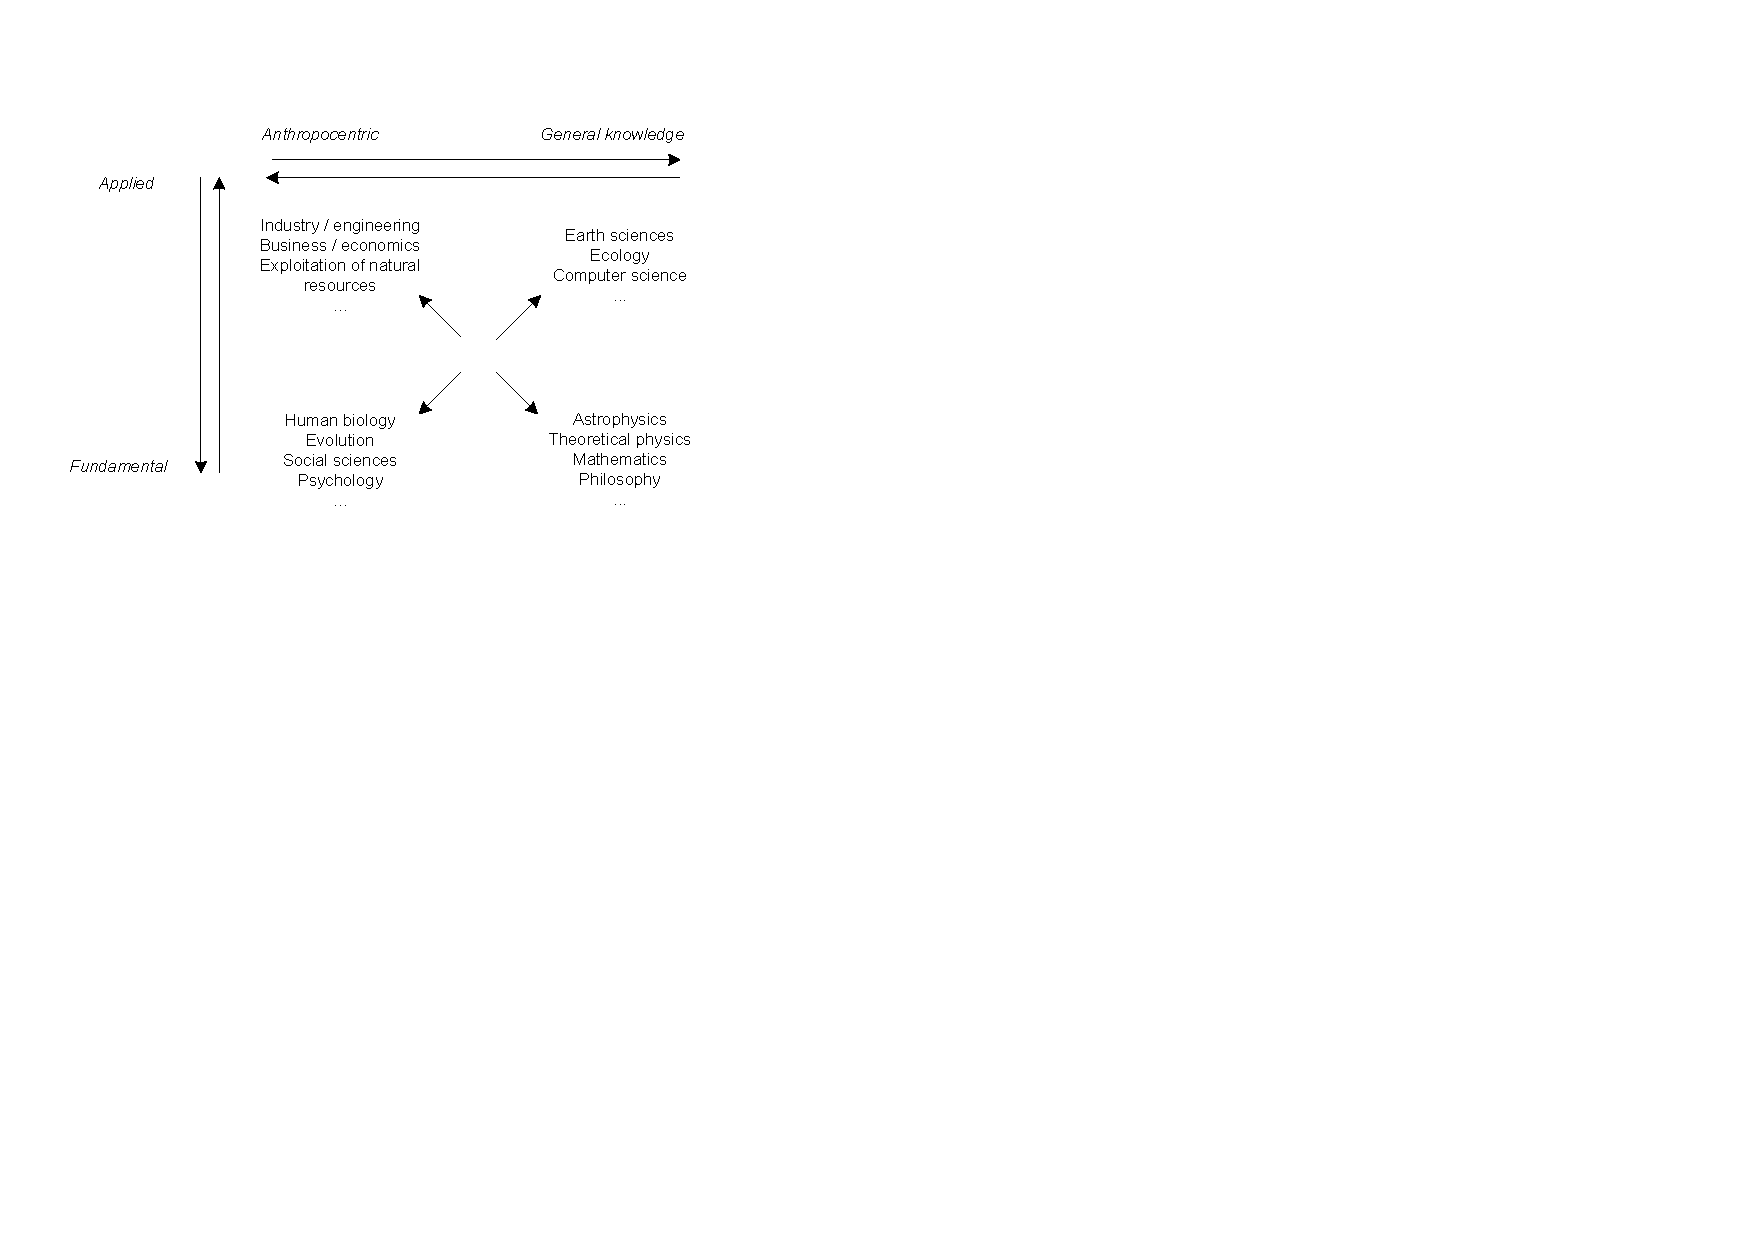
\includegraphics[width=.9\textwidth]{Fig_science_fields.pdf}
\caption{One possible 2D high-order classification of science.}
\label{Fig:science_fields}
\end{center}
\end{figure*}


A broader view on science is that it is a complete human system consisting of \emph{scientific products}\index{research article!introduction} (data, information, knowledge, laws, theorems, algorithms, and scientific articles and books), \emph{researchers} (people who professionally conduct research experiments), \emph{research groups} (teams of researchers working on similar topics and meeting regularly at scientific meetings and workshops), \emph{legal entities} (research societies, institutes and schools, national and international organizations with their members, structures, formal rules and evaluation criteria), and \emph{commercial companies} that sell or trade in scientific products (publishers and other providers of scientific information).\index{scientific!information} \par

At the highest level, scientific fields can be classified as a) \emph{formal} or theoretical and b) \emph{applied}, although such distinctions are rather fuzzy. Another major split in science is that between \emph{natural} and \emph{social} or behavioral sciences (see also Fig.\@~\ref{Fig:science_fields})\index{science!classification}.\par

\begin{figure*}[!htb]
\begin{center}
  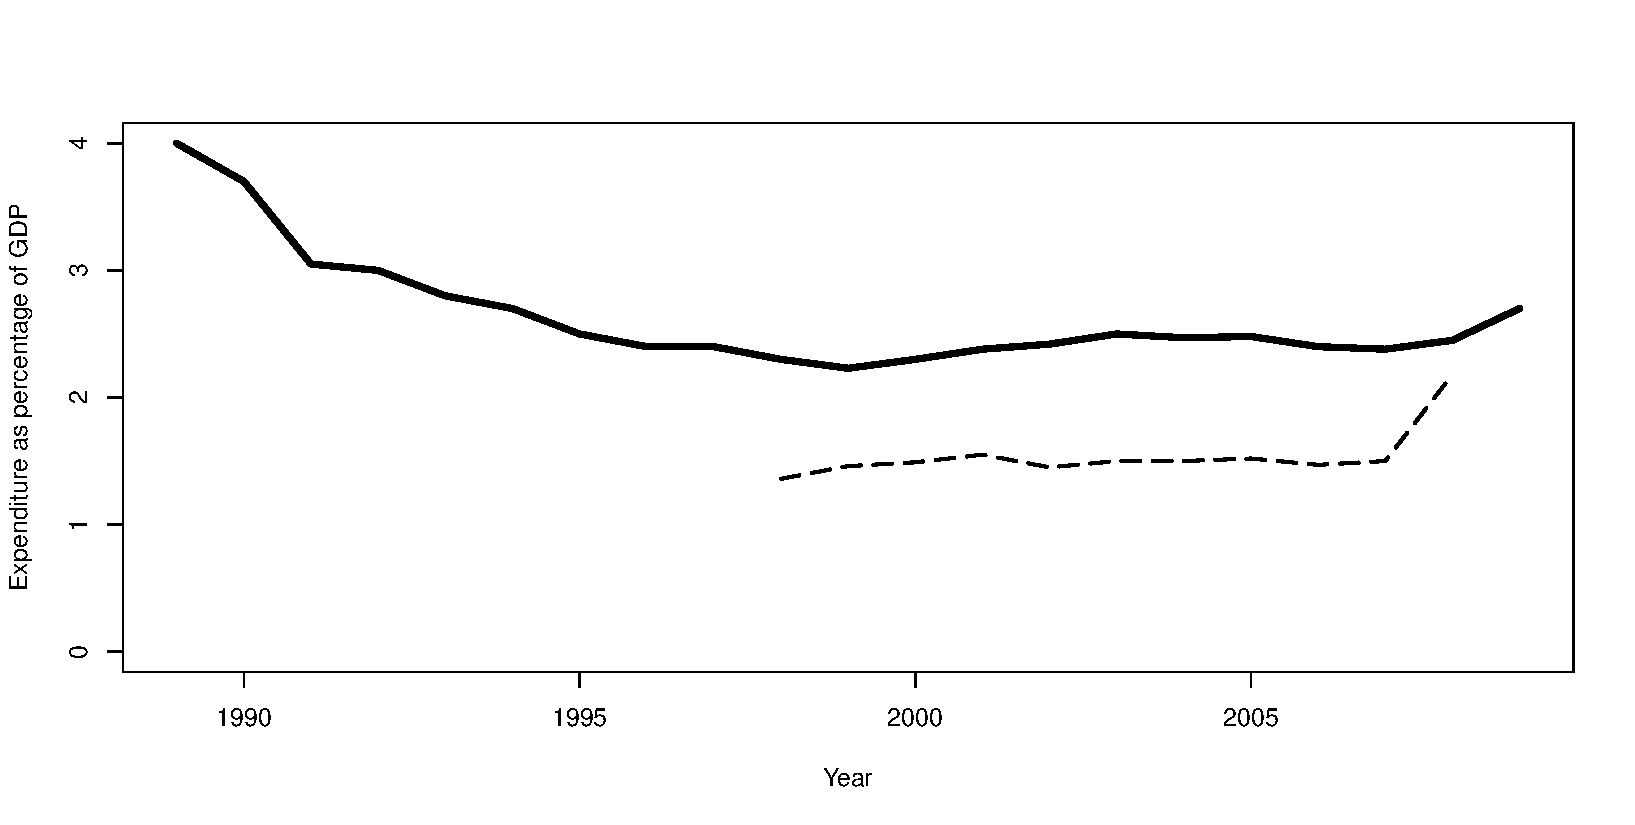
\includegraphics[width=\textwidth]{Fig_world_expenditure.pdf}
\caption{Military (bold line) and research \& development (broken line) expenditure as a percentage of GDP (World data). Data source: World Bank, World Development Indicators and \href{http://statinfo.biz}{\texttt{statinfo.biz}}.} \label{Fig:world_expenditure}
\end{center}
\end{figure*}

The contemporary view of science is that the classification of people into (a single) research field is rather old-fashioned and that groups should strengthen their \emph{multi-} and \emph{inter-disciplinarity}\index{inter-disciplinarity} through collaboration with other (thematically) distant groups and through combinations of professionals within a single group. The focus in science should be on solving research problems and reporting research in a systematic way and not on formal relationships between and within the fields. Nevertheless, many government organizations insist on research classifications\footnote{For example, the Australian Government (\url{http://www.abs.gov.au}) requires every research proposal to be linked to a specific research field, discipline, and clear socio-economic objectives, i.e.\@ national research priorities.}. Standardization of science makes it easier to organize research applications, find reviewers and link one's work with research priorities. \par

Not all research fields receive the same degree of support or funding. Unfortunately, many research fields that attract large sums of money are on the edge of being classified as science\footnote{For example, secret military experiments receive far more funding than public benefit/democratization projects such as the One Laptop Per Child or \textsc{Wikipedia}.}\index{One Laptop Per Child}. Likewise, people spend much more money on producing medication to treat obesity than on research on healthy nutrition or protecting endangered species. We have still not reached a level of civilization where more money is spent on research and development than on weapons (Fig~\ref{Fig:world_expenditure}). Just to give you a rough figure, the Watson Institute\footnote{\url{http://costsofwar.org}} has estimated that the costs of the USA military intervention in Iraq and Afghanistan are between 3.2--4~trillion US\$ (!). Imagine if this money was spent on research and education instead. \par

\begin{figure*}[!hbt]
\begin{center}
\resizebox{.9\textwidth}{!}{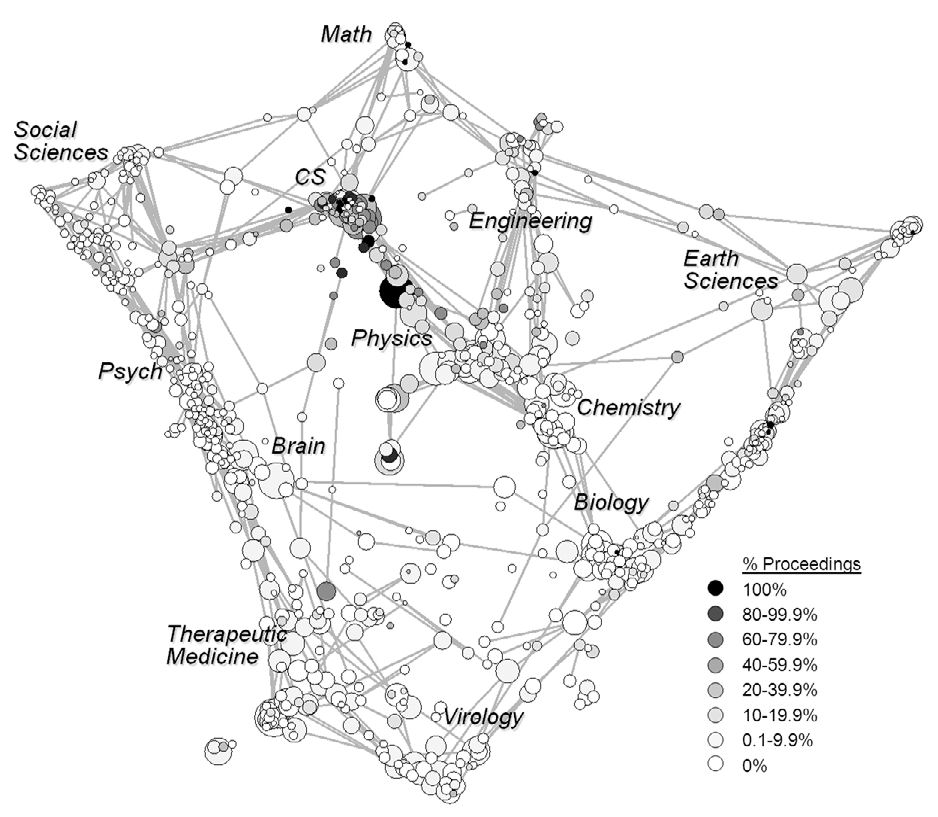
\includegraphics{Fig_Boyack_2009_map_of_science.jpg}}
\caption{Graphical representation of major scientific fields according to \citet{Boyack2009Scientometrics}: disciplinary map including SCIE, SSCI and Proceedings databases. Each node (circle) is a cluster of journals and is sized to show numbers of papers by cluster. With permission from Springer Science+Business Media.}
\label{Fig:map_of_science}
\end{center}
\end{figure*}

Should every researcher strive to achieve multidisciplinarity? Researchers live, create and move around within what are often closed circles (research fields), which have their own rules and principles. Isolation of scientific fields in contemporary science is considered to be old-fashioned, but it still happens. For Howard Gardner\footnote{\url{http://www.howardgardner.com}} hyperdisciplinarity\index{hyperdisciplinarity} or looking at everything through one discipline is an example of a poorly disciplined mind: \emph{``Economists who see the whole world through rational choice; psychologists who see the whole world through evolutionary psychology; the lawyer who sits down with his children who are two and three years old and writes down a constitution which gives the children their rights and their responsibilities.''} \par

\begin{center}
 \resizebox{\textwidth}{!}{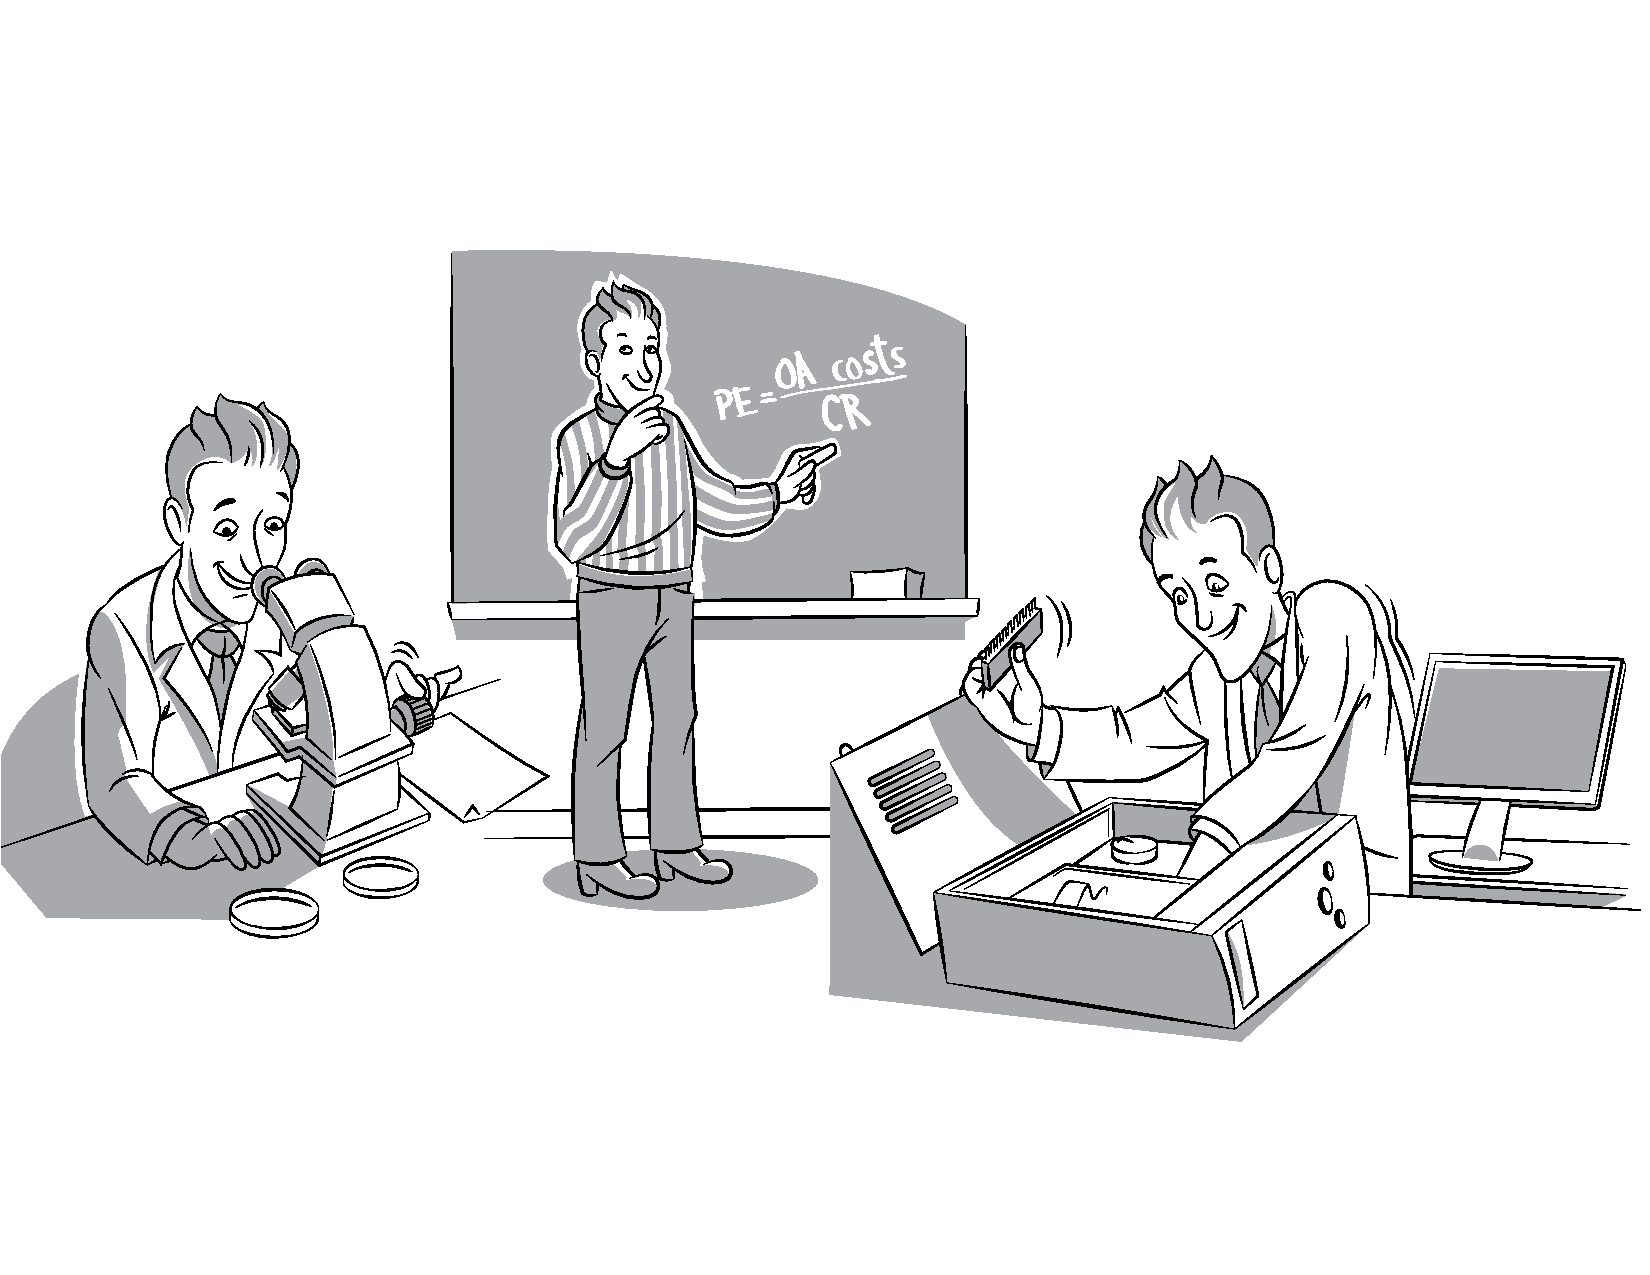
\includegraphics{Fig_scientists.pdf}}
\end{center}

Fig.\@~\ref{Fig:map_of_science} shows a (disciplinary) map of some major scientific fields based on numbers of publications in the Science Citation Index Expanded (SCIE) /, Social Sciences Citation Index (SSCI), and Proceedings databases \citep{Boyack2009Scientometrics}. This shows that many research groups are clustered within a field or sub-field, which is probably related to the way universities, research institutes and journals are organized --- faculties and departments are often isolated; graduates then go on to work in professional associations, which have their own unions and even political lobbies. Each field may have its own principles and people in authority. Fig.\@~\ref{Fig:map_of_science}\footnote{There are several similar world maps of science; e.g.\@ by \citet{Bollen2009PLOS}.} shows the impact of political priorities on science.\par


\section{Scientific information}


\textbf{Scientific information}\index{scientific!information} is the collective name for any type of written, physical or multimedia record of scientific work. For practical reasons, the products of research work (research projects) are typically split into one or more stand-alone items (\emph{scientific information packages}) which are used to convey a new concept or discovery to a research community (except in the case of a review article, in which authors attempt to systematize existing knowledge). Scientific information packages are usually published in written media --- as journal articles, books or book chapters, websites, but also increasingly in multimedia, including videos and interactive websites and programs. Popular explanations of scientific information are then often communicated more widely through television and the print media. \par

\begin{svgraybox}
The process of producing and disseminating scientific information is called publishing. Scientific information (packages) are usually published in written media --- as journal articles, conference proceedings, technical reports, textbooks and/or book chapters.
\end{svgraybox}\label{R:publishing}

Scientific information evolves during the research process. Research\-ers start with some rough ideas and initial data and then build these up into standardized products (publications, multimedia materials) that are searchable through commercial or open indexing systems. The role of commercial companies is to register, certify, distribute/promote and archive scientific information.\par

\bigskip
\begin{fminipage}{.9\textwidth}{\footnotesize{\textsf{\textbf{On copyright and authorship}} --- Copyright\index{copyright} is the exclusive right granted by the law of a jurisdiction to the product owner to copy, distribute and make profits. Copyright should not be confused with \emph{``authorship''}\index{authorship} --- the right of a person or group of people who developed an original product (the creators). Authors make intellectual property (IP) that is automatically copyrighted. This may be their own property, or it may belong to the organization that finances their work (it's often specified in employment contracts). A good example: Paul McCartney wrote music for the Beatles  and Michael Jackson bought the copyright. Authors can transfer their copyright to individuals or commercial companies. By transferring the copyright, authors no longer \emph{`own'} their intellectual creation\index{intellectual property} and need to request permission to copy and distribute it according to a licence agreement. In most countries copyright ceases after 70 years after the death of the author. Authorship is non-transferable. In many legal systems around the world authorship also includes some rights. For example, a publisher with a copyright on some work has no right to alter, modify or blank out the original authors' names. In most legal systems the main concern is the copyright, which gives its holder the right to financial benefits.
}}
\end{fminipage}
\bigskip

In more general terms, there are at least five forms of scientific information products:

\begin{itemize}
  \item \emph{Unprocessed products}: raw data, development versions of algorithms, notes and sketches.
  \item \emph{Draft products} (test beds): development versions of information systems, technical reports, draft documents, beta versions of packages (new software and/or technology).
  \item \emph{Pre-prints} (no peer review, no editing): submission-ready products, rigourously tested versions of information system, scientific documents (articles) and beta versions of software packages. Publication of pre-prints allows scientists to get new work out quickly, although with limited credibility.
  \item \emph{Published products} (peer reviewed, edited): licensed (standard) scientific products that are indexed in scientific databases i.e.\@ those with a patent number, Digital Object Identifier (DOI), ISBN or similar.
  \item \emph{Promotional by-products}: media packages developed to support the promotion of scientific information --- slide shows, websites, newspaper articles, documentaries, pubcasts, and videos.
\end{itemize}

These are the basic evolutionary stages of scientific information. Commercial companies are typically only interested in submission-ready papers that can be prepared and copyrighted as commercial products. Researchers, on the other hand, work with scientific information products at all stages. In this book we present guidelines for how to produce all of the products listed above. \par

The process of producing and disseminating scientific information is called publishing\index{publishing!models}. There are three major publishing models:

\begin{enumerate}
\renewcommand{\labelenumi}{\textit{\Roman{enumi}}}
  \item \emph{Commercial (toll-access) publishing} --- The author transfers the copyright to the publisher in exchange for professional distribution. Copyrighted materials are sold in bulk or in parts. Copyright infringement is regulated by law and subject to financial sanctions.
  \item \emph{Open access (subsidized) publishing} --- Authors or their organizations pay\footnote{In some situations publishers might give up the right to profit and provide open access free of charge.} publishers to \emph{open} the copyright and make the materials available free on-line. There are three versions of Open Access (OA) publishing\index{Open Access!publishing}:
      \begin{enumerate}
        \item \emph{Author-pays OA} --- the costs of OA are paid by the author.
        \item \emph{Organization-pays OA} --- the costs of OA are paid by an academic and/or government institution.
        \item \emph{Delayed OA} --- the article is made available for free download after a fixed period of time, which is usually longer than one year\footnote{At an International Federation of Science Editors conference in Merida, Mexico in 2004, a doctor pointed out to an Elsevier executive that \emph{``by the time you make information available at a price I can afford, my patient is dead.''}}.
      \end{enumerate}
  \item \emph{Open (non-commercial) publishing} --- All materials (manuscript and the review process) are copyrighted under public domain. These can be freely distributed without limitation.
      \begin{enumerate}
        \item \emph{Organization supported} --- production and printing are supported by an organization.
        \item \emph{Self-publishing} --- production and printing are organized solely by the authors.
      \end{enumerate}
\end{enumerate}

Note that the annual subscription to a specialist medical journal can cost the price of a small car; author-pays OA can also cost a significant amount of money (see further page~\pageref{Tbl:publishing_models_comparison}).\par

\section{Why do we write research articles?}

Have you ever asked yourself what the essence of a research article is? Is it merely a report on an experiment or is it an essay or a user guide for colleagues who would like to conduct similar research? In fact, a research article is a bit of all of these. It looks like a research report, but it also contains some unique spices: belletristic elements similar to those in an essay or article in a magazine. However, unlike essays, research articles need to follow a logical structure and provide all technical details. They must be rigorous because they have a practical purpose --- to communicate the results of research in a systematic and standardized way.\par

\begin{svgraybox}\index{research article!purpose}
The purpose of a research paper is to communicate the results of research --- new, original findings (new concepts, new data) --- in a systematic and standardized way so that readers can apply, modify and extend that knowledge.
\end{svgraybox}\label{R:func}

People have different reasons for publishing their research. First, there is prestige --- researchers aim to be the first to explain or solve an important problem. Second, by solving some research problem we get a chance to improve peoples' daily lives \emph{``at scales expanding human lives''} \citep{AscheronKickuth2004}. Third, there is the intellectual exercise, which helps us to express our creativity. Intellectual creations can be intrinsically valuable. \par

Although researchers also communicate their ideas at conferences, meetings and through the educational system, their contribution to science is mainly measured through research output in publications. Many researchers in the history of science who did not publish their work are no longer connected with that work\footnote{The classic example of a researcher who \emph{perished} is Christian Huygens, who may well have been a superior scientist to Descartes or even Newton, but did not seriously consider publishing his work \citep{Crump2002}.}. This is nicely illustrated by the well-known aphorism \emph{publish or perish}. To some extent, this gives scientific work a competitive character --- scientific discoveries are connected with those who first publish them (in a high-impact journal). That's the name of the game.\par

Publication of your ideas/discoveries is not (at least it should not be) the ultimate ambition of a researcher. The most important thing for a researcher is to make a significant contribution to science, i.e.\@ to make an impact. So the true motto of a researcher should in fact be: \emph{publish and make an impact or perish}.\par


\section{Research quality}

By publishing their research, scientists expose themselves to critical evaluation. The scientific quality\index{research quality} of a research article is typically a product of: (1) the quality of the design of the experiment, (2) the quality of arguments/proofs, (3) the quality of methods and materials, and (4) the quality of the presentation of the research results (see Fig.\@~\ref{Fig:what_makes_good_paper}). Scientific quality is difficult to evaluate before publication. Researchers need time (sometimes even decades) to look at someone else's work and find out what its real advantages are. That's probably why the Nobel Prize is awarded to researchers toward the end of their careers (the median age of Physics Nobel Prize recipients is 51).\par

Retrospectively, scientific quality can be measured as the effect of a number of professional achievements:

\begin{itemize}
  \item \emph{Proven impact on the world of science} (good citation statistics)
  \item \emph{Proven general interest in your work} (invitations to give keynote speeches and lectures, number of articles in the media)
  \item \emph{Grants received and research funding}
  \item \emph{Professional awards received} (e.g.\@ best paper awards).
\end{itemize}

Although these are very concrete measures, they are not easy to collect and update. In fact, the managers of most research organizations do not really know what the performance of their employees is, how established the people in their teams are, and what their performance trend is. Evaluating researchers' performance is usually outsourced to scientific information and consulting companies. The most accepted way of tracking authors' impact is through the tracking and analysis of citations.\par

\bigskip
\begin{fminipage}{.9\textwidth}{\footnotesize{\textsf{\textbf{Bibliometrics}}\index{bibliometrics} --- a subfield of scientometrics --- is a set of methods that's used to monitor bibliographic information i.e.\@ library items. By monitoring the citation statistics of research publications we can compare the productivity and impact of different authors and institutes and discern trends and clusters. Several bibliometric indices can be used to track researchers and their output. The most widely used are: $h$-index for authors, Impact Factor ($\rm IF$) for journals, and Citation Rate (CR) and Relative Impact Factor (RIF) for articles. Nowadays, thanks to Google Scholar, SCImago Lab, ResearcherID and other open access web services, anyone can track articles and see which publications, authors and journals are really \emph{`hot'}. For more details about state-of-the-art bibliometric indices see e.g.\@ \citet{Harzing2010}.}}\index{Harzing}
\end{fminipage}
\bigskip

Once an article is published, it starts accumulating \emph{`points'} i.e.\@ citations. This is the absolute measure of its impact. Of course, it's not fair to compare the number of times a 15-year-old paper has been cited with the impact of the work of a \emph{`rookie'}. Citations need to be normalized e.g.\@ by dividing them by article age and by the research field.\par

An objective measure of the impact of a paper is the average number of annual citations --- its \textbf{Citation Rate}\index{citation rate} (CR) \citep{Garfield1990CC}:

\begin{equation}\label{E:CR}
   CR = \frac{{\rm total} \; {\rm number} \; {\rm of} \; {\rm citations}}{{\rm years} \; {\rm since} \; {\rm publication}}
\end{equation}

CR is commonly filtered for self-citations. A further modification of the CR is citation rate per author (CRpA), which normalizes for the number of authors for each paper \citep{Harzing2010}.\par\index{Harzing}

By dividing the citations by the average citation number in a research field one can derive the \textbf{Relative Impact Factor} (RIF):\index{relative impact factor}

\begin{equation}\label{E:RI}
   RIF = \frac{{\rm total} \; {\rm number} \; {\rm of} \; {\rm citations}}{{\rm average} \; {\rm number} \; {\rm of} \; {\rm citations} \; {\rm in} \; {\rm the} \; {\rm field}}
\end{equation}

For example, papers in environment and ecology receive an average of 11.35 citations (Fig.\@~\ref{Fig:ESI_world}\footnote{Based on \url{http://researchanalytics.thomsonreuters.com}}). This means that a paper that receives 20 citations has an RIF of 1.76.\par

\begin{figure*}[!hbt]
\begin{center}
\resizebox{\textwidth}{!}{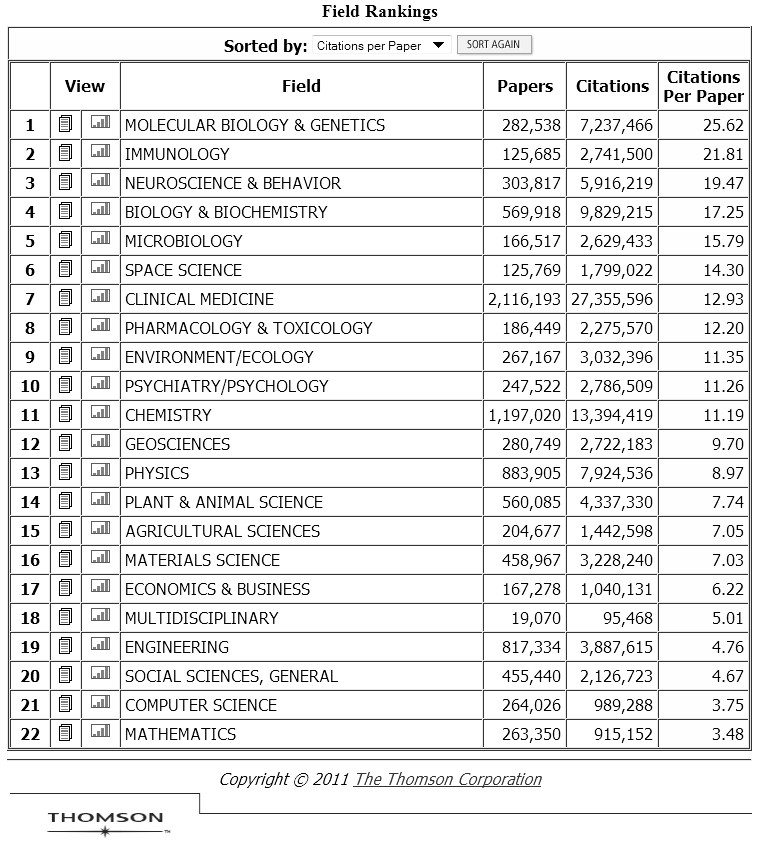
\includegraphics{Fig_ESI_world.jpg}}
\caption{Field rankings table based on Essential Science Indicators data (a bibliometrics product by Thomson Reuters).}
\label{Fig:ESI_world}
\end{center}
\end{figure*}

Most articles gradually disappear from references, which means that they have a citation \emph{`half-life'}: the number of years that one has to go back in time to account for 50\% of the total references \citep{Garfield1990CC}. In Natural Sciences, the citation half-life typically ranges from 3-10 years, although most articles will only be cited during the first few years (if at all).\par

\begin{svgraybox}
An objective evaluation criteria of the impact of a research article is its Citation Rate --- the number of times it has been cited per year. Citations can be further standardized per research field using global averages to estimate the Relative Impact Factor.
\end{svgraybox}

A publication's citations plotted on a time line approximately follow the asymmetric (Hubbert) curve: they will first grow exponentially, reach a peak, and then follow a decay function (Fig.\@~\ref{Fig:citations_h_index}a). Unlike books, which can be updated periodically in new editions or updated continuously online (like this book), research articles get a permanent bibliographic reference and tend to have a limited life. With exception of Scholarpedia, which promotes the idea of having \emph{live} articles --- on-line articles which are continuously updated by article \emph{curators}.\par

Unfortunately, many publications have almost no life at all i.e.\@ they never get cited. Most researchers will only write a handful of publications that make a real impact in their field. If we sort an author's publications according to the number of citations, we obtain a graph such as that shown in Fig.\@~\ref{Fig:citations_h_index}(b).\par

\begin{figure*}[!hbt]
\begin{center}
\resizebox{\textwidth}{!}{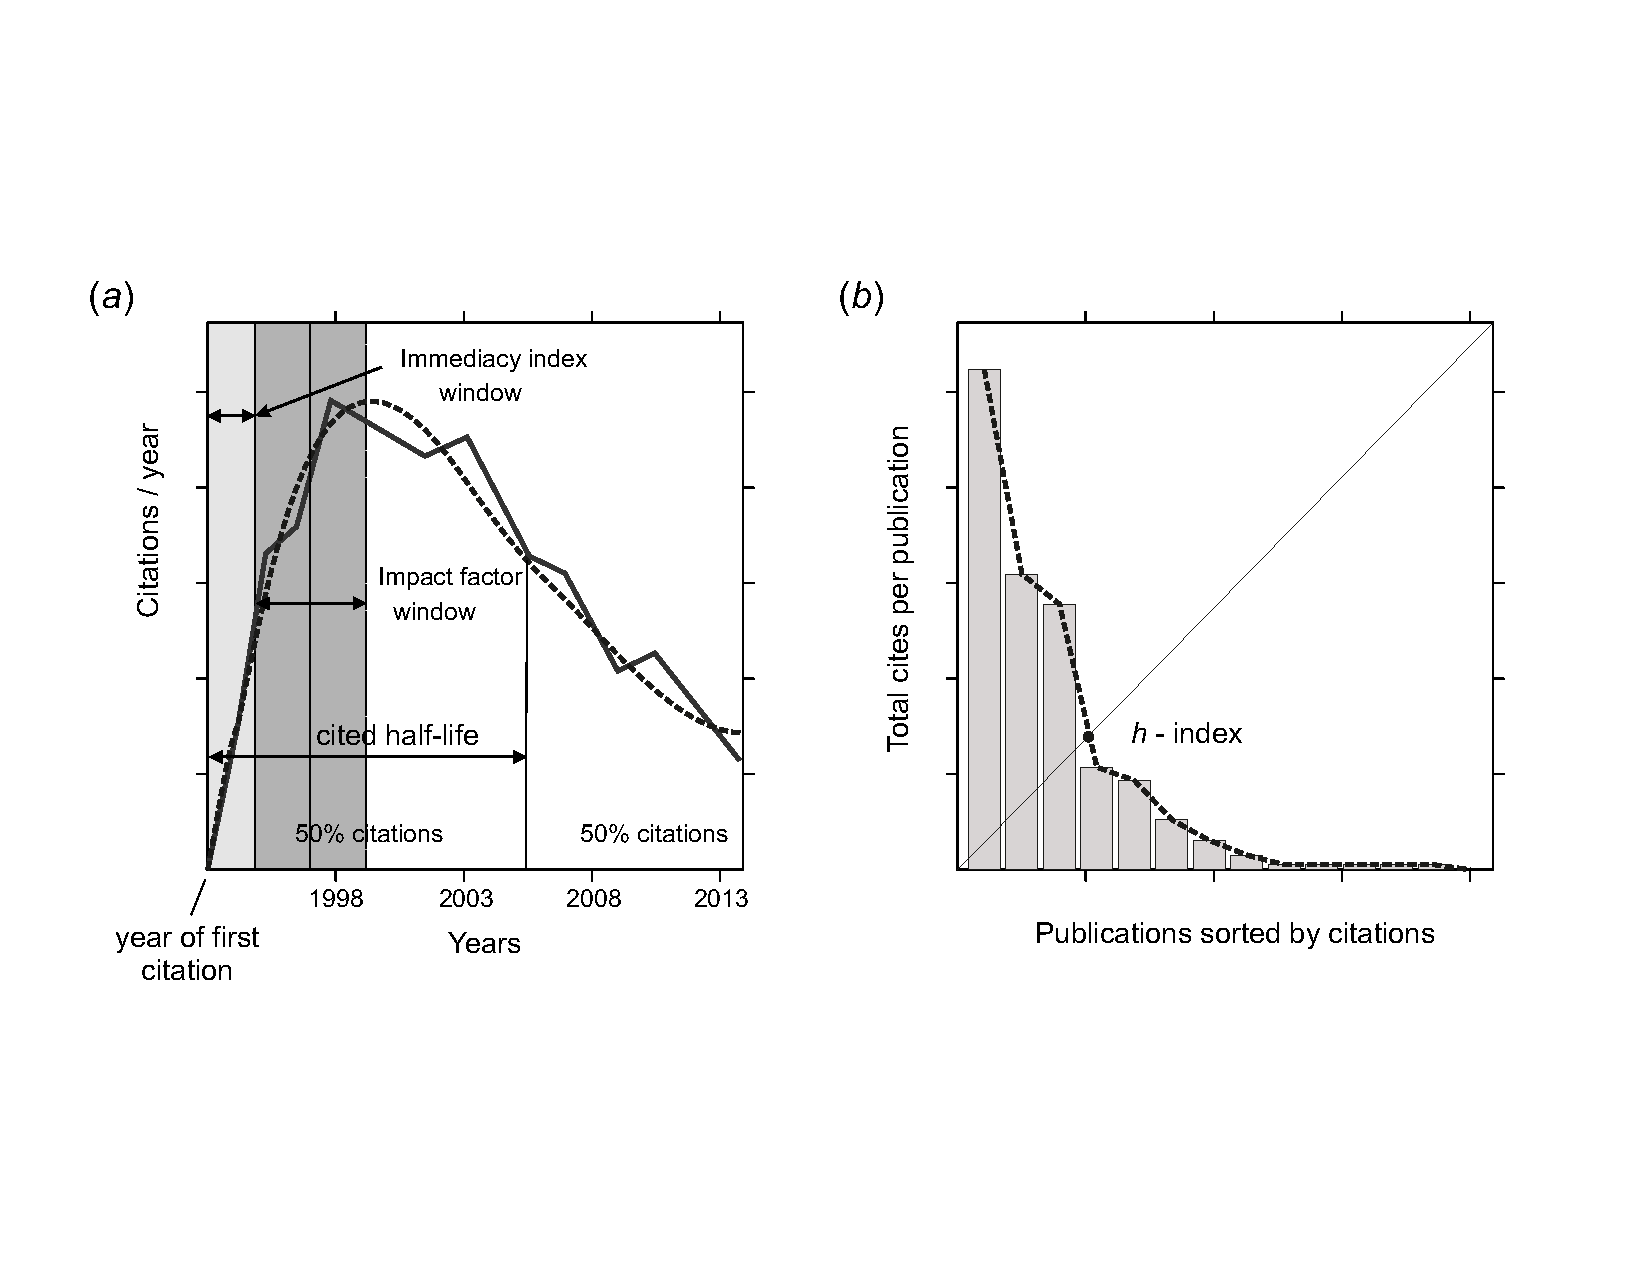
\includegraphics{Fig_citations_h_index.pdf}}
\caption{Basic principles of citation analysis: (a) an article's life visualized using citations per year; (b) the derivation of the $h$-index.}
\label{Fig:citations_h_index}
\end{center}
\end{figure*}

In order to track scientists' output using a single measure, \citet{Hirsch2005} proposed a simple citation index that was then named ``$h$-index'' after Hirsch's name. An \textbf{$h$-index}\index{h-index@$h$-index} is derived from the number of an author's papers that are cited at least $h$ times (see Fig.\@~\ref{Fig:citations_h_index}). The $h$-index is more suitable for evaluating authors because it corrects for \emph{``one-hit wonders''} --- academics who have authored only a small number of highly-cited papers \citep{Roediger2006AO,Harzing2008AM,Bar-Ilan2008scientometrics}.\par

An author with a high $h$-index has delivered a durable academic performance. The $h$-index is basically designed to distinguish truly influential scientists from those who simply publish many papers. The problem is that it is a function of the scientific age of an author and it may be much smaller for relatively young authors who might be writing just as good articles as their senior counterparts. \par

The third common bibliometric measure is the Impact Factor\index{Impact Factor}\index{Journal's Impact Factor} (IF), which is defined as:

\begin{equation}\label{E:IF}
   IF (t) = \frac{ \begin{matrix}
{\rm number} \; {\rm of} \; {\rm times} \; {\rm articles} \;  {\rm published} \; {\rm in} \; {\rm year} \; t_{-2} \; {\rm and} \; t_{-1} \\
{\rm which} \;{\rm were} \; {\rm cited} \; {\rm by} \; {\rm indexed} \; {\rm journals} \; {\rm in} \; {\rm year} \; t
\end{matrix} }{ \begin{matrix}
{\rm total} \; {\rm number} \; {\rm of} \; {\rm citable} \; {\rm items} \\
 {\rm published} \; {\rm by} \; {\rm that} \; {\rm journal} \; {\rm in} \; {\rm year} \; t
\end{matrix} }
\end{equation}

IF is a bibliometric measure that was developed primarily for evaluating journals, i.e.\@ to derive a Journal's Impact Factor (JIF)\index{JIF|see{Journal's Impact Factor}}. JIF has received a lot of criticism from researchers and research organizations for various reasons. First, often many articles, even in journals with a high impact factor, are almost never cited \citep{Seglen1997BMJ}. Research on Nature's 2004 impact factor, for example, has shown that about 90\% of its IF was based on only a quarter of its publications \citep{Editorial2005N}. Second, journal issues are artificial entities. Articles in a journal issue are independent, even when they come in special issues. To mix the achievements of people who have most probably never even heard of each other is like mixing apples and oranges (as the plot in Fig.\@~\ref{Fig:JIF_vs_RAI} left illustrates). Third, a journal can adopt editorial policies that artificially increase its impact factor. \citet{PLoS2006} warn that a consequence of basing the evaluation on JIF is that \emph{``science is currently rated by a process that is itself unscientific, subjective, and secretive.''}\par

\begin{figure*}[!htb]
\begin{center}
  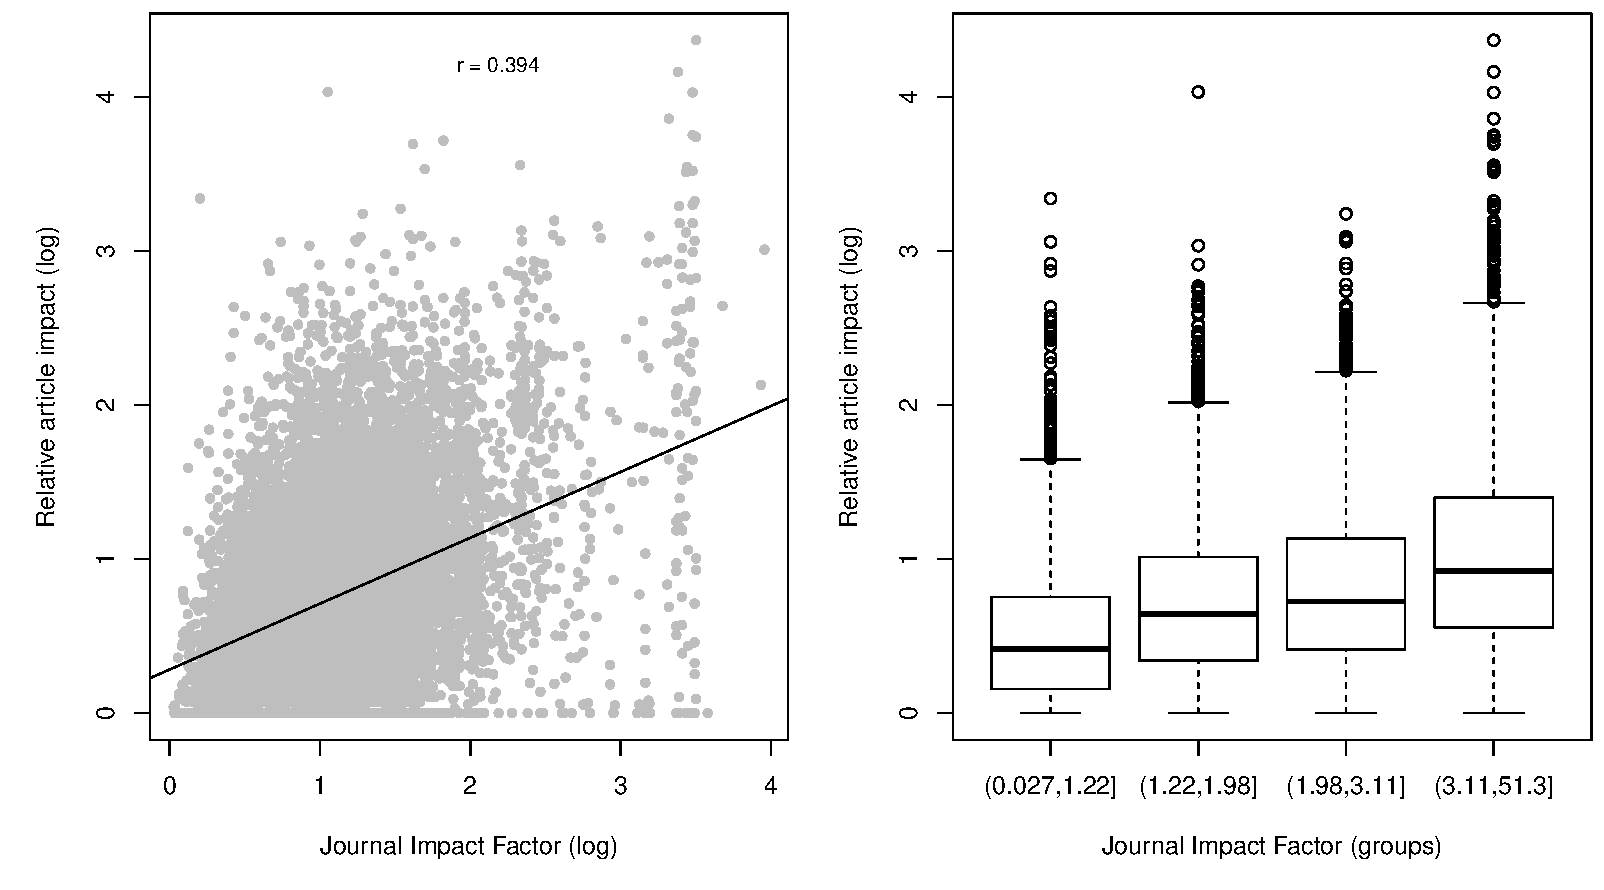
\includegraphics[width=\textwidth]{Fig_JIF_vs_RAI.pdf}
\caption{Journal impact factors and individual relative impact factor (Eq.\ref{E:RI}) for 14,348 articles published at Wageningen University in the period 2002-2009. JIF explains only 14\% of the variability in the RIF. The original data can be obtained from the Wageningen University Library.} \label{Fig:JIF_vs_RAI}
\end{center}
\end{figure*}

Unfortunately, JIF is still by far the evaluation criterion that's most widely used by government and funding agencies \citep{Adler2009}. If you plan to send an application for a scholarship or funding, there's a good chance that evaluation of your proposal will be primarily based on the IF of the journals in which you published your work. \par

\begin{svgraybox}
JIF is often incorrectly applied to evaluate the significance of an individual publication or an individual researcher. However, if you submit an application for a scholarship or grant, there's a good chance that the evaluation of your proposal will be primarily based on the JIF related to your publications.
\end{svgraybox}\label{R:impactfactorgame}

\begin{figure*}[!htb]
\begin{center}
  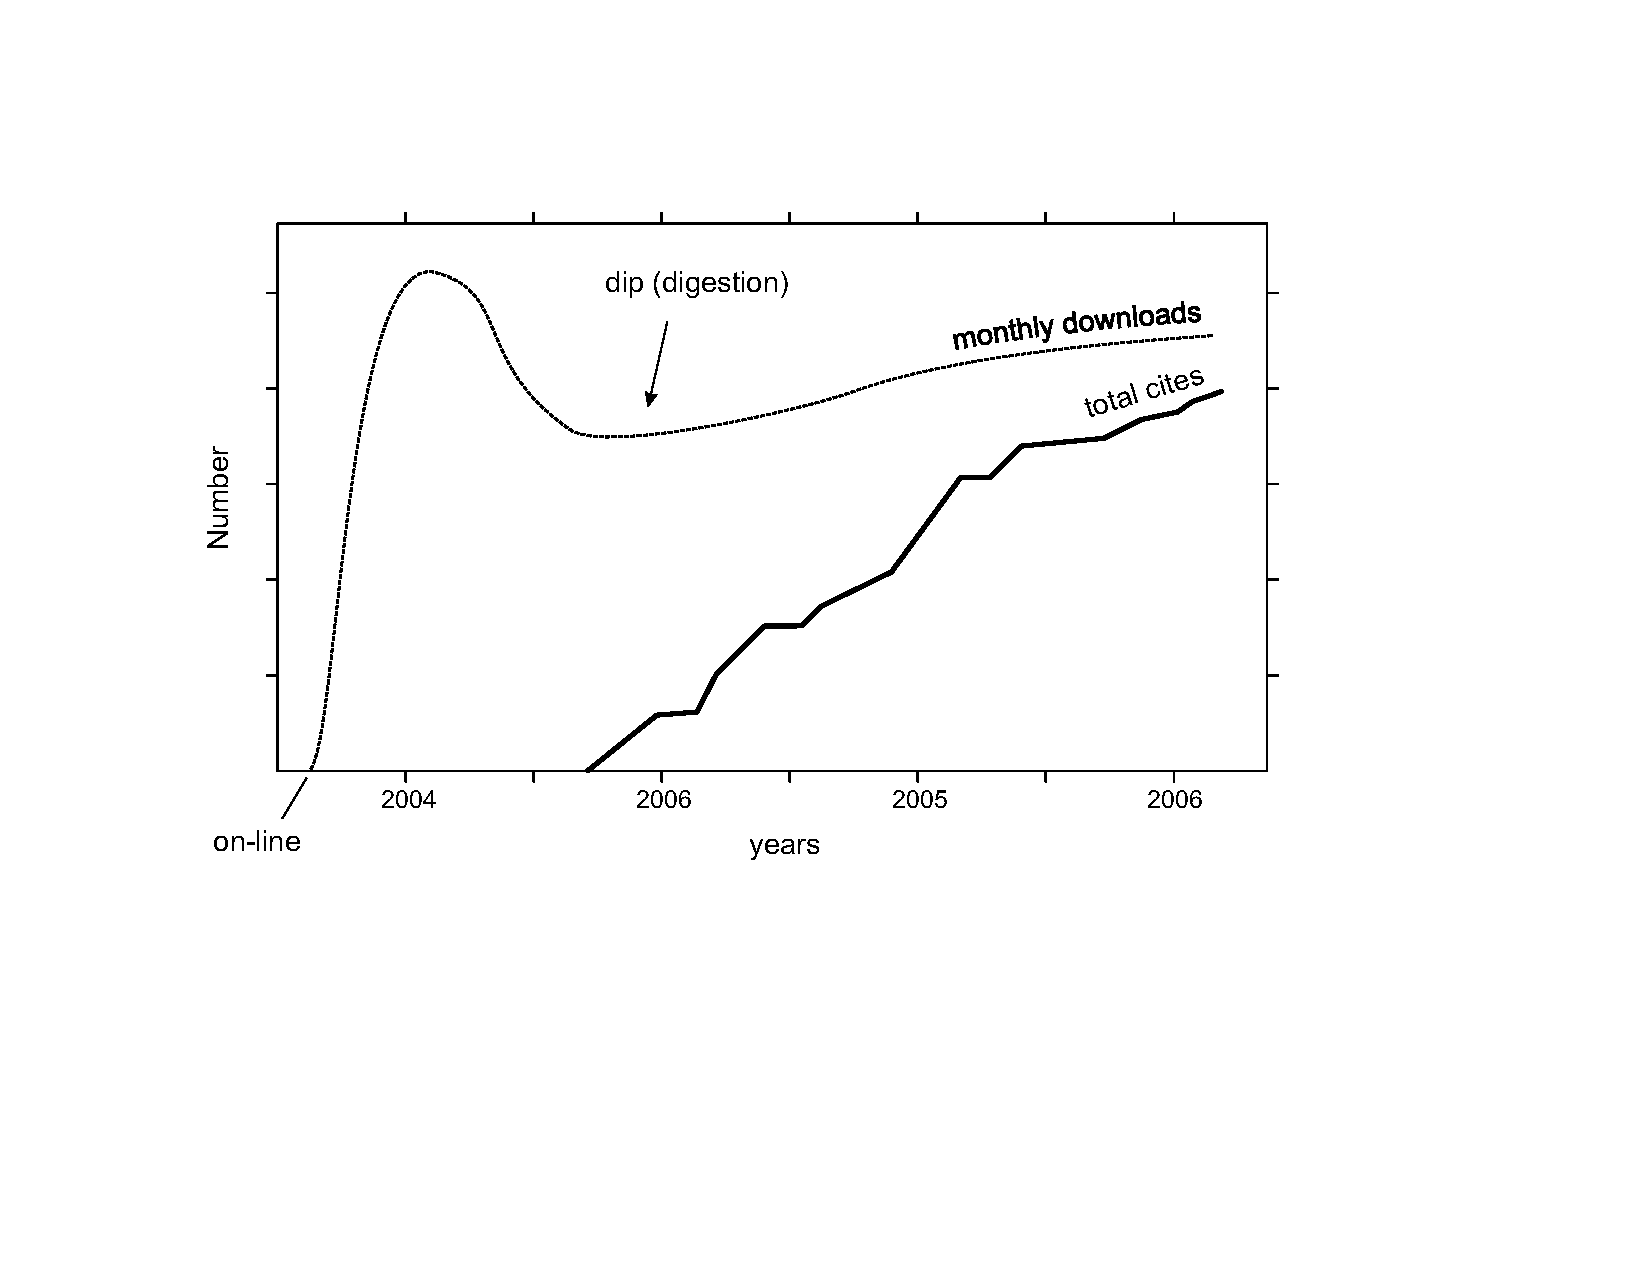
\includegraphics[width=.8\textwidth]{Fig_cites_vs_downloads.pdf}
\caption{Schematic example of download (or paper access) statistics versus citation statistics. Although download statistics and citations are likely to be correlated, citations are typically delayed for 2-3 years; likewise, the most downloaded papers do not necessarily influence citations.} \label{Fig:cites_vs_downloads}
\end{center}
\end{figure*}

Nevertheless, work by \citet{LariviereGingras2010} has shown that duplicate papers published in higher-impact journals obtain, on average, twice as many citations as their identical counterparts published in lower impact factor journals. Hence high IF journals do make a difference (see also Fig.\@~\ref{Fig:JIF_vs_RAI} right), and journals with a JIF in the upper quantile do perform better on average. \citet{LariviereGingras2010}:

\begin{quote}
\emph{``The intrinsic value of a paper is thus not the only reason a given paper gets cited or not, there is a specific Matthew Effect attached to journals and this gives to papers published there an added value over and above their intrinsic quality.''}
\end{quote}

In other words: publishing in high-impact journals is good, but using JIF as a measure of the quality of individual articles is controversial. \par

The good news is that bibliometrics are slowly changing towards more diverse, more web-based measures. PLoS has recently introduced \emph{``article-level metrics''} --- a list of measures that focus on individual merits, rather than on the journal's impact factor. These include\footnote{\url{http://www.plosone.org/static/almInfo.action}}:

\begin{itemize}\renewcommand{\labelenumi}{(\textit{\alph{enumi}})}
  \item Citation statistics by third-party citation measuring services (Scopus, PubMed Central, and CrossRef)
  \item Number of article views / visitor statistics (PDF, HTML, XML format of documents)
  \item Social bookmarks at Delicious, CiteULike and Connotea
  \item Comments and notes, blog activity, article rankings and other similar types of web activity.
\end{itemize}

Web-based measures will play an increasingly important role in bibliometrics.\par


\section{Bibliometric services}

Nowadays the impact and importance of research publications, journals, and authors can be successfully followed through web services, the three best known of which are:

\begin{itemize}
   \item \textbf{Web of Knowledge}\index{Web of Knowledge}\index{bibliometrics!services} (\href{http://webofknowledge.com}{\texttt{webofknowledge.com}}) --- is a Thomson Reuters' Scientific subscription-based multidisciplinary database that covers about 9000 peer-reviewed journals clustered in the following three databases: the Science Citation Index Expanded, Social Sciences Citation Index Expanded and Arts and Humanities Citation Index. The v4.0 of Web of Knowledge indicates that it contains about 23 million full documents from the period 1988--2011. Web of Knowledge can generate citation reports and be used to analyze the results, e.g.\@ to compare the success of authors, institutes or countries, and to see how paper citations change over time. The results of searches can be exported in a variety of formats and used to generate reports. Web of Knowledge is the most detailed and most accurate scientific database of peer-reviewed articles published in the English language (but available only by subscription).
  \item \textbf{SCOPUS}\index{SCOPUS} (\href{http://scopus.com}{\texttt{scopus.com}}) --- Elsevier's SCOPUS (also subscription-based service) contains around 33 million abstracts from about 16,000 peer-re\-view\-ed journals, but also shows the status of non-registered SCOPUS publications, including 386~million web-based publications. SCOPUS has recently offered a Citation Tracker service that makes it possible to assess impact of an individual author/publication. The $h$-index is now also incorporated in SCOPUS and can be derived for each selected author/group. A limitation of SCOPUS is that it does not contain citation information for articles published before 1996.
  \item \textbf{Google Scholar}\index{Google Scholar} (\href{http://scholar.google.com}{\texttt{scholar.google.com}}) --- GS is a non-comme\-rcial academic search service that registers publications available on the web. It indexes all on-line materials, including PowerPoint presentations, mailing lists, blogs and such-like, but also all peer-reviewed journals that are available on-line (except those published by Elsevier). The advantage of Google Scholar is that it allows free searches for publications written in any language and from any publisher and thus contributes to the democratization of citation analysis \citep{Harzing2008ESEP,Harzing2010}. Google Scholar has been available since 2004 and its quality is continually improving. Its biggest limitations are noisy data, inconsistencies, duplicate publications, and errors. Microsoft now also provides an academic search service called \textbf{Microsoft Academic Research}\footnote{\url{http://academic.research.microsoft.com}}\index{Microsoft Academic Research}.
\end{itemize}

Each of these web services has its advantages and disadvantages and each offers something that its competitors do not have. They clearly compete with each other in providing key information about citation records and there will always be differences --- some minor, some significant.\par

\citet{Bauer2005DLIB}, for example, showed that there is not much difference between GS and Web of Knowledge in terms of the accuracy of assessing the number of citations for highly-cited publications, but there is indeed a significant difference between GS and Web of Knowledge / SCOPUS in assessing all publications within a certain field. \citet{Meho2007JASIST} estimated that the overlap between the results of GS and Web of Knowledge / SCOPUS is only 30--50\%. This happens typically because GS indexes about twice as many publications as Web of Knowledge / SCOPUS, including conference papers, dissertations, theses, and book chapters. As Google's database grows, this difference is becoming smaller and smaller \citep{Harzing2010}. \par

\begin{sidewaysfigure}[!hbp]
\begin{center}
  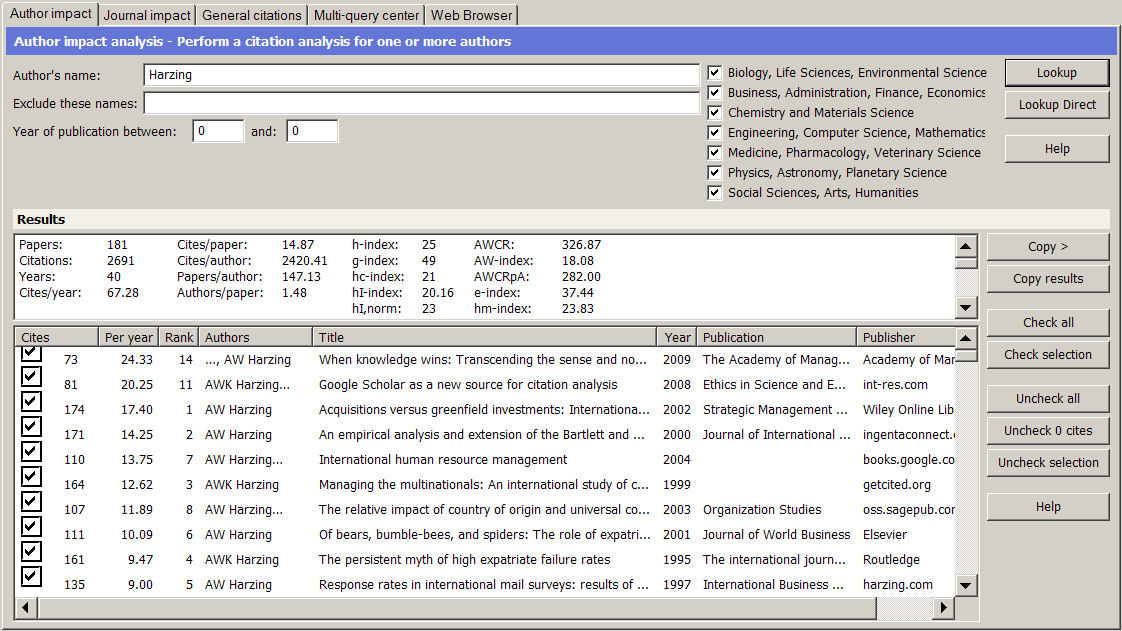
\includegraphics[width=.85\textwidth]{Fig_PoP_on_Harzing.jpg}
\caption{\textsf{Publish or Perish}\index{software!\textsf{Publish or Perish}} is a small freeware application, that allows searches of the Google Scholar database and citation analysis \citep{Harzing2010}.\index{Harzing} A similar ranking service for journals is the SCImago Journal and Country rank service.} \label{Fig:PoP_on_Harzing}
\end{center}
\end{sidewaysfigure}

Although there has been pressure for academic organizations to start using GS, many librarians advise sticking to Web of Knowledge or SCOPUS if you need an accurate citation count \citep{Giles2005Nature}. This is mainly because GS is often incomplete and noisy. In addition, Google refuses to reveal details of its search algorithm, although this may change in the near future. \par

Most international publications can also be browsed using the \textbf{WorldCat}\index{WorldCat} service\footnote{\url{http://worldcat.org}}, which is provided by the OCLC Online Computer Library Center\index{Online Computer Library Center}, Inc. This web service contains over 1 billion items from more than 10,000 libraries. It allows you to search bibliographic items by title, subject and/or author's name. The query results are grouped by authors, research fields, formats, languages and year of publication. WorldCat can also sort query results by publication date and relevance. Each book, article, report, audio or video material receives a unique OCLC number. However, it does not (yet) provide any bibliometric evaluation of publications.\par

The world's largest internet bookshop \textbf{Amazon}\index{Amazon} also does not provide any scientometric measures. However, it does allow sorting of books by popularity (\emph{sort by best selling}), which can be as important as the most sophisticated bibliometric index.\par

Nowadays, scientists can also be traced by geographical location. Springer hosts a service called \textsf{AuthorMapper}\footnote{\url{http://www.authormapper.com}} that shows a geographical distribution of authors and their work (actually it is a space-time visualization) --- an excellent way to find out where the scientific hot-spots are. Unfortunately, as with many commercial companies, the results of searches are typically limited to Springer-connected or Springer-owned products. \par

The main problem of bibliometrics is that scientists do not have a unique international identifier, something like an ISBN for books. At the national level, certain countries have organized some kind of registry, at least for people working for government organizations. These registries are not compatible at the international level, which is clearly inefficient. Many authors have the same names (even with two middle letters), many change locations, some change names, etc.\par

To account for this, SCOPUS uses an \textbf{Author Identifier}\index{author identifier}, but this is then linked to the hosting institution. For example, the first author of this book has several identifiers:

\begin{verbatim}
    AU-ID("Hengl, Tomislav" 6602864740)
    OR AU-ID("Hengl, Tomislav" 13409408400)
\end{verbatim}

\noindent where \texttt{ID 6602864740} refers to the period when the author worked at the ITC in Enschede, the Netherlands and \texttt{ID 13409408400} to the period when he was an employee of the JRC at Ispra in Italy. Furthermore, SCOPUS allows users to group the same authors with multiple identifiers. Web of Knowledge does not make this distinction --- it only keeps the most recent address in the database. On the other hand, an advantage of Web of Knowledge is that it allows users to zoom into research articles and observe how citations change for each article. \par

Especially people with \emph{`van'} and \emph{`der'} prefixes are in a difficult situation because they could lose out in the citation rankings just because they are cited inconsistently in different publications. For Jackie Senior (a science editor at the UMC in Groningen), the worst example so far is certain Dr.\@ Johannes Kristian Ploos van Amstel, also know as Hans Kristian P van Amstel, HK van Amstel, J van Amstel, and many other combinations. Performing a complete bibliometric analysis with such inconsistent author names is very cumbersome. The name ambiguity problem is probably one of the most serious problems of bibliometrics at the moment.\par

\begin{sidewaysfigure}[!hbp]
\begin{center}
  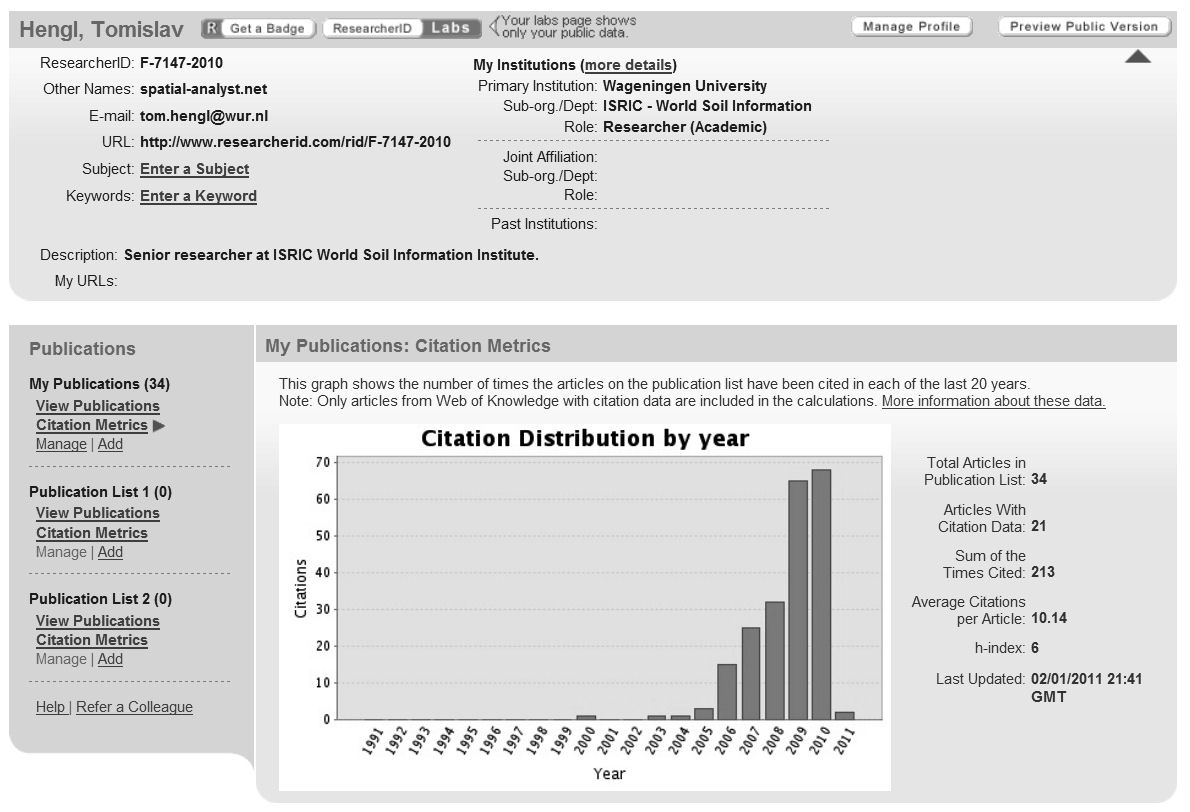
\includegraphics[width=.8\textwidth]{Fig_citation_metrics_Hengl.jpg}
\caption{Example of complete citation statistics as reported by ResearcherID.} \label{Fig:citation_metrics_Hengl}
\end{center}
\end{sidewaysfigure}

Another example of a global registry of researchers is \textbf{ResearcherID}\footnote{\url{http://www.researcherid.com}}\index{ResearcherID} from Thomson Reuters (free service). In August 2011 this contained records from over 100,000 scientists around the globe. ResearchID provides a unique ID for each researcher, which is available via a URL, for example:

\begin{verbatim}
http://www.researcherid.com/rid/F-7147-2010
\end{verbatim}

The ResearcherID entries are further linked to ISI publications, which are sorted by total number of citations (Fig.\@~\ref{Fig:citation_metrics_Hengl}). The problem with ResearcherID is that authors are responsible for setting up and updating their profile, so the total number of researchers in the system is still low.\par

Like Google Scholar, Microsoft Academic Research also crawls the web and generates researchers' profiles in a semi-automated manner. Microsoft uses a 7-digit number:

\begin{verbatim}
http://academic.research.microsoft.com/Author/1876597
\end{verbatim}

Unlike with SCOPUS, information about researchers from Google Scholar and Microsoft Academic Research (including citation statistics) is publicly available and hence can easily be queried from the web. Moreover, Google and Microsoft allow anyone to edit the author details to ensure accurate data. \par

To minimize duplication and errors, unique identifiers such as Digital Object Identifier\index{DOI|see{Digital Object Identifier}} (DOI) and ISBN for books will increasingly be used. Similar universal identifiers probably need to be introduced for authors and other library items, such as computer programs and maps. \par

It would be great to have a unique web-based database, which anyone could use to check the correct reference of all library items in the world at any time. Open and efficient bibliometrics and scientometrics registries would certainly contribute to the democratization of science and weaken the monopolistic positions of some scientific information indexing companies. Although Google seems to be closest to reaching this goal, probably some truly non-profit international association such as the Online Computer Library Center\footnote{\url{http://www.oclc.org}} would be a better choice.\par

Another non-profit organization set up to solve the problem of author name ambiguity is ORCID Inc\footnote{\url{http://www.orcid.org}}. ORCID is building a global database of researcher IDs, which link each author to their IDs in SCOPUS, Web of Knowledge, ResearcherID and similar author databases. Ultimately, we only need one ID in science.\par

Examples of web services for maintaining and/or cross-linking bibliographic records are \textbf{PublicationsList}\footnote{\url{http://publicationslist.org}} and CrossRef\footnote{\url{http://www.crossref.org}}\index{CrossRef}. Such services allow researchers and research organizations to maintain a reliable web-based record of their academic output. If you already have some publications, you should register them on ResearchID.com and/or PublicationsList.org and thus contribute to building a global registry of authors and publications.\par


\section{From draft manuscript to peer review}\label{sec:filtering}

The process of getting your work evaluated is called \textbf{peer review}\index{peer review} or refereeing. Peer review is a critical examination of your work by established researchers in the field --- usually the journal's reviewers. Based on the degree of anonymity, reviews can be divided in:

\begin{enumerate}
  \item \emph{Blind} --- authors do not see the names of referees (i.e.\@ anonymous reviews).
  \item \emph{Double-blind} --- authors' and referees' names are hidden.\index{double-blind review}
  \item \emph{Personalized} --- authors' and referees' names are known.
\end{enumerate}

For most editorial offices, the results of reviews are often left unpublished --- stored in an internal database or recycled. There is much debate in the academic world about \emph{`open'} and \emph{`closed'} refereeing and publishing models. For example, Prof.\@ James Hartley, Research Professor in the School of Psychology at the University of Keele (widely known for his work on student learning, text design and academic writing), believes that, especially in the information age, reviewing should be open i.e.\@ the authors should know the names of referees and \emph{vice versa}: \emph{``little --- if anything --- should be hidden from different contributors to the total system''}. Read more about such debates on page~\pageref{sec:publishing_models}. \par

Review is a filtering process: experienced established researchers help you improve your paper so that it meets certain quality criteria. Filtering scientific publications involves the following specialized operations:\label{page:filtering articles}

\begin{description}
  \item[\emph{Checking for general suitability}] \hfill \\
  Journal or book editors quickly browse your document and check if it is of interest to the journal, submitted in the required style and structure, and contains no nonsense. This type of gross-error filtering generally takes very little time. You could compare it with the spam filter in your e-mail manager. However, it's crucial that the editor gets the point of your research very quickly. According to Professor Edwin Gale\footnote{Editor of Diabetologia, as reported by Ed Hull in a workshop on Advanced Science Editing on February 18, 2011.}: \emph{``I receive about 15 articles per day. Most of them I reject within 3 minutes. The main reason for rejecting them is that I do not see the point of the research.''} Similarly, John R.\@ Benfield wrote in the Journal of Medical English Education: \emph{``Thirty years of service as an editor and reviewer have taught me that imperfections or errors in grammar are rarely, if ever, responsible for the rejection of a manuscript. Manuscripts are rejected because they lack new information, new ideas, clarity and credibility.''} \medskip
  \item[\emph{Cross-checking the scientific content}] \hfill \\
  In the next phase, journal editors invite (at least) 2-3 experienced scientists who specialize in a similar field or sub-field to focus on the scientific content more closely and evaluate the originality and quality of your methods and writing. This is probably feasible within several days, but because reviewers do this work voluntarily, they are usually given a few months to respond. \medskip
  \item[\emph{Cross-checking the data analysis and results}] \hfill \\
   Ideally, each paper submitted for publication that contains some type of statistical analysis or summaries of results should be checked for accuracy and typos in the code. Recall the Rules of Science from page~\pageref{F:rules}: anybody should be able to reproduce your results. This is not considered to be the responsibility of a journal --- publishers make it clear that they are not responsible for the accuracy of numbers or graphs. In fact, data analysis steps are often kept secret, both for objective and subjective reasons. For example, many large software companies keep their code and data \emph{closed} for commercial reasons i.e.\@ to protect their copyright. \medskip
  \item[\emph{English language editing}] \hfill \\
   The communication quality of text can usually be considerably improved. An English language editor does not necessarily need to be an expert in the field, although it is much more efficient if he/she has at least some general knowledge of the topic. Language experts can edit text endlessly, but our concern is not to have a perfectly written paper --- simply to have a document that is readable, clear, concise, well-organized and credible\footnote{British and USA embassies organize the certified English language exams IELTS and TOEFL, which are often used by universities as admission criteria; The EU has published a Common European Framework of Reference (CEFR). An author submitting a paper to a journal should pass the \emph{``proficient users''} of English level (at C2 on the CEFR Global Scale) or better.}. Journals and book publishers rarely invest in language editing. In more than 90\% of cases readability is left to the authors. \medskip
  \item[\emph{Editing graphics}] \hfill \\
   A figure in a research article can potentially become better known than the article itself. Charts not only inform, but also can be used to persuade and even campaign\footnote{\url{http://www.economist.com/node/10278643}}. Producing artwork is costly, so it is (unfortunately) often left to the authors, who usually lack design skills (see further section~\ref{sec:supergraphics}; page~\pageref{sec:supergraphics}). \medskip
  \item[\emph{Page proofs}] \hfill \\
   Final polishing of the document --- prepared as \emph{Camera Ready Copy}\footnote{Although an outdated term, CRC is still used for digital documents that are ready for printing or press-ready.} (CRC) --- is often referred to as correcting the \emph{``Page proofs''} or proofchecking. Now the author has very little time (24 to 48~hours) to read the document one more time line by line and make corrections. The focus at this stage is on typos, wrongly ordered tables and graphs and minor errors in the text.
\end{description}

As reported in a December 2010 article in Nature, entitled \emph{``A helping hand''}, Jim Viccaro, editor of the Journal of Applied Physics, routinely recommends editing services to authors: \emph{``Reviewers these days are overburdened, and a properly written paper is just easier to review,''} he says. Prices, which vary according to the level of service, the length of the paper and the turnaround time, can be anything from 250 US\$ for a 6,000-word paper with a 14 to 21--day turnaround to 5000 US\$ for a 12,000-word paper with a 48-hour turnaround.\par

Viccaro sees it is a worthwhile investment: \emph{``This is how an author can make sure their paper is not dismissed for the wrong reason, just because no one could understand what they were talking about,''} he says. In the same article, Xiao-Fan Wang, an associate editor at the Journal of Biological Chemistry, maintains that directing non-English-speaking authors to editing companies before submission has allowed him to accept an extra 5 to 10 percent of papers that he would otherwise have rejected. \emph{``These services can offer a lot of value,''} he says. \emph{``Not only in terms of the English, but in highlighting what the author didn't even realize was the most important part.''}\par

So to get a document from \emph{Limbo} to \emph{Purgatorio} and on to divine purity often requires expertise from a number of professionals. Unfortunately, researchers often do not have graphic designers, language experts, marketing or IT gurus in their teams. You should at least be aware of what's needed to deliver a polished product and, where necessary, bring in the missing expertise.\par


\section{Types of articles}\index{research article!classification}

Generally speaking, there are three main types of published scientific articles:

\begin{itemize}
  \item \emph{Original research articles}
  \item \emph{Review articles}
  \item \emph{Popular articles} (or research articles adjusted to target a specific audience)
\end{itemize}

In this book we focus on designing and producing original research articles, i.e.\@ complete technical information packages representing original new findings. Writing review articles and popular science articles requires different skills from those needed to produce original research articles \citep{turabian2007manual}. \citet{MonteroLeon2007} go further and suggest a classification system for studies in psychology, with three main groups:

\begin{enumerate}\renewcommand{\labelenumi}{\textit{\Roman{enumi}}}
  \item \emph{Theoretical studies}:
    \begin{enumerate}
      \item Classical reviews
      \item Meta-analysis
    \end{enumerate}
  \item \emph{Empirical quantitative studies}:
      \begin{enumerate}
        \item Observational descriptive studies
        \item Survey descriptive studies
        \item Experiments
        \item Quasi-experiments
        \item \emph{Ex post facto} studies
        \item Singe case studies
        \item Action research
      \end{enumerate}
  \item \emph{Empirical qualitative studies}:
       \begin{enumerate}
         \item Ethnography
         \item Case studies
         \item Instrumental studies
       \end{enumerate}
\end{enumerate}

In similar fashion one could classify studies in various broad research fields (and would possibly come up with a similar classification system).\par

Another way to classify articles is based on their production costs. Anything you produce could potentially be published; the question is often: how many copies should be distributed? \citet{Smith1990TR} suggests that there are basically three groups of articles:\index{types of articles}\index{article, types} (1) those with limited results, which are nevertheless surprising and might spark new research (\emph{publish}), (2) papers which mostly repeat work by others (\emph{these should not be published}), and (3) papers which present good ideas, but are badly expressed (\emph{these should not be accepted, but the authors should be encouraged to rewrite and thus make them more comprehensible}).\par

\begin{figure*}[htb]
\begin{center}
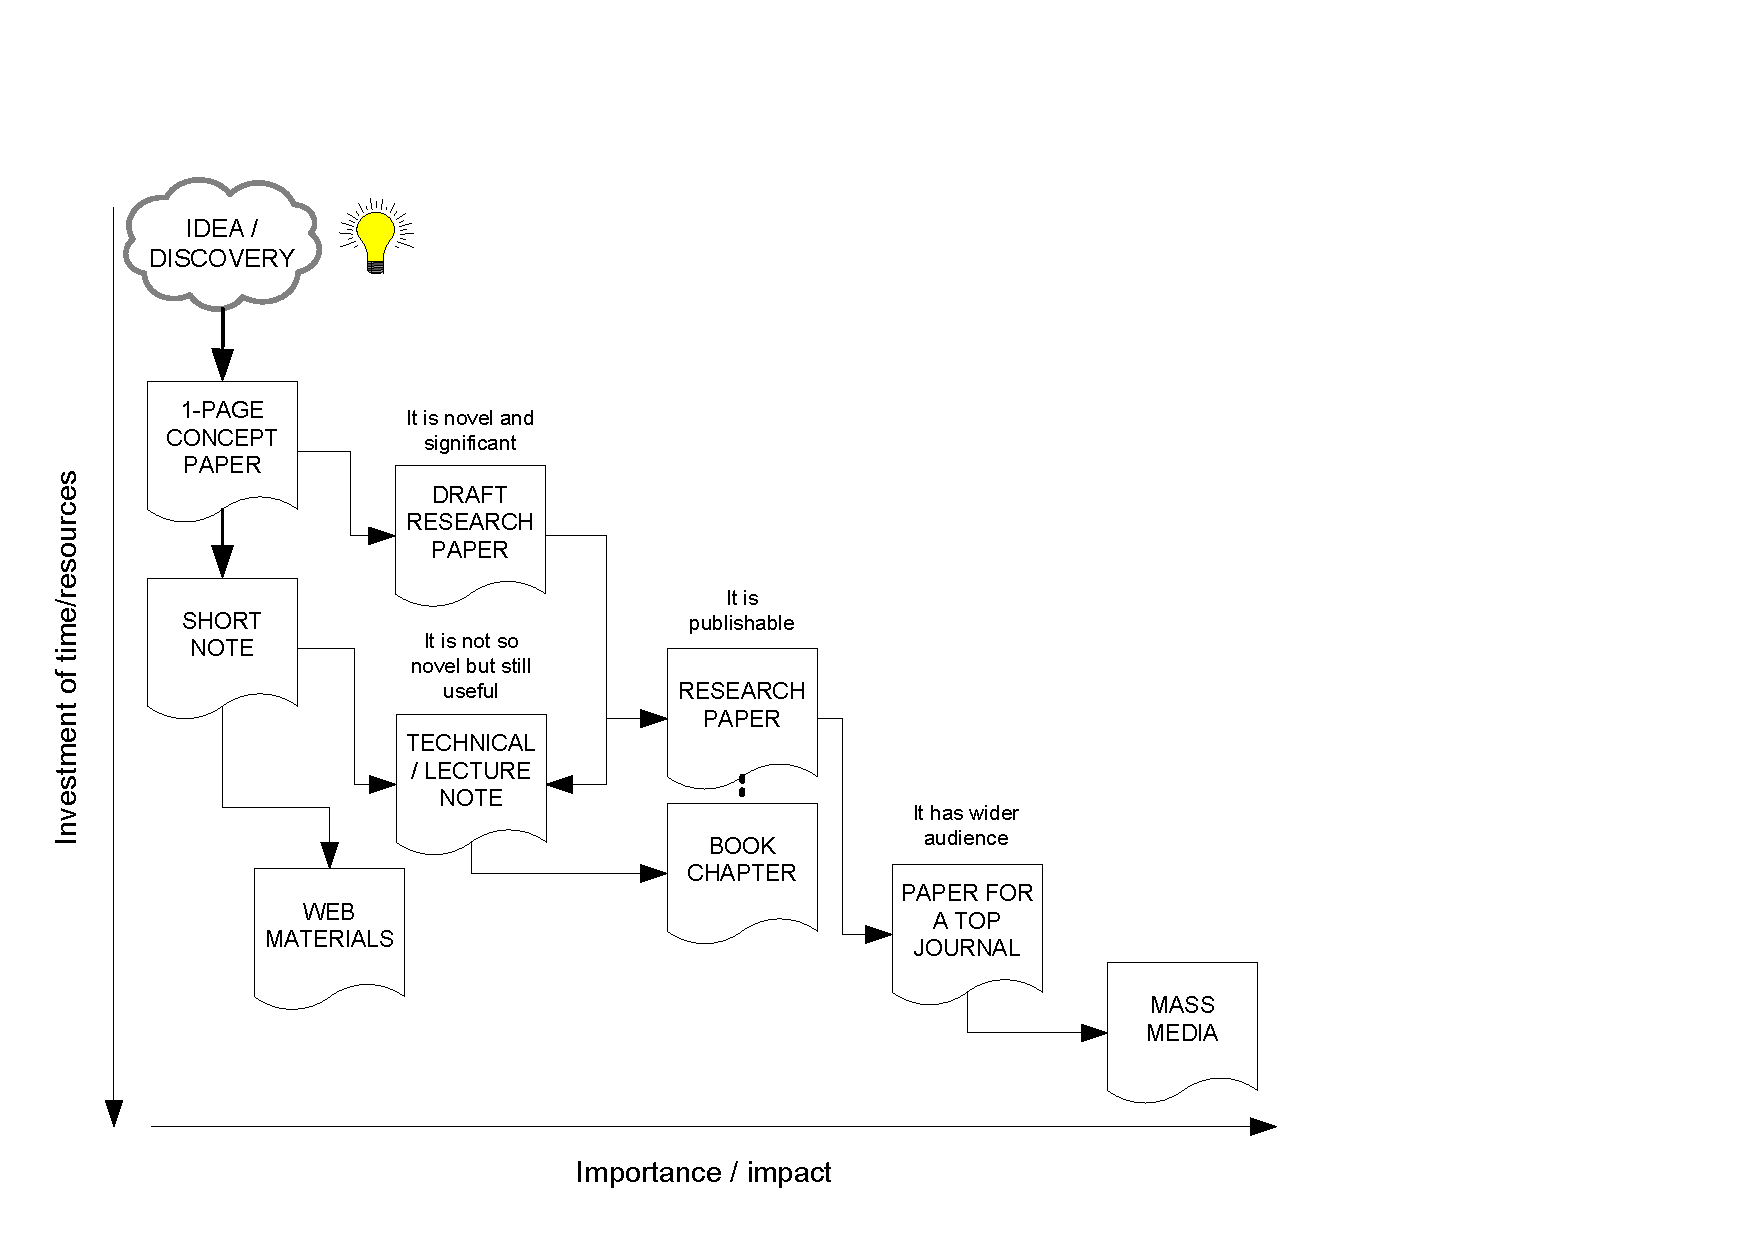
\includegraphics[width=.9\textwidth]{Fig_publications.pdf}
\caption{Types of publications in relation to investment of time/resources and potential impact. Ideas evolve or devolve based on the feedback we get from the audience.}
\label{F:pubs}
\end{center}
\end{figure*}

Based on how often an article is cited, we can roughly distinguish the following five categories of published articles:

\begin{description}
\item[\emph{Born-dead} papers]  \hfill \\
     These are papers that are almost never cited. Their citation half-life is infinitely short, which means that the topics discussed do not have an audience, the paper is `indigestible' or it's simply dull. Some papers are simply \emph{bad science chasing a bad idea}, but it takes time until the research community forms an opinion on this. Some might argue that such papers are simply a waste of resources, but this is not completely true. A small proportion of born-dead papers have great potential (\emph{`sleeping beauties'}), but they are too avant-garde, too introspective or too hypothetical. So, it is worth having a record of some good ideas even if we do not exactly know what they mean and how they can be used to solve real-life problems. The real problem is that about two-thirds of all papers belong to this \emph{`born-dead'} category \citep{Garfield1979S,Latour1987S}. \medskip
\item[\emph{Proving-the-known} papers]  \hfill \\
     Many papers are reasonably well-written, based on excellent data and the whole project seems to be well organized and conducted, but they are simply not significantly novel (others have already done the work). They can often still be useful, because they retell known theory in a more \emph{`digestible'} way or they are more effective in providing a bigger picture. A paper needs to successfully transfer useful knowledge. So, if an author thinks that he/she can do a much better job then the original author, such a paper will be welcomed. Of course, the author needs to search for and acknowledge the original work (dig into the literature), even if he/she is not initially aware of it.\medskip
\item[\emph{Promising} papers]  \hfill \\
     These are the papers that reveal new discoveries/ideas that are significant for both experimental and applied science. Sometimes, even a badly written paper can be promising. Unlike the \emph{born-dead} and \emph{proving-what-you-know-papers}, authors of promising papers show both talent and dedication to science. Also consider the fact that research groups usually need at least a few years to absorb the ideas laid out in a paper, so such promising papers can eventually get promoted to a higher class.\medskip
\item[\emph{Most-cited} papers]  \hfill \\
     The most cited \citep{Garfield1990CC} or the most downloaded papers are those that have not only proved to be promising, but also those that the research community has shown most interest in. Such papers usually distinguish leading scientists\footnote{See for example \url{http://isihighlycited.com}.}\index{ISI Highly Cited} from \emph{run-of-the-mill} ones. In many cases, the most frequently downloaded papers do not need to be of exceptionally high quality (they do not even need to have immediate practical implications), but they should nevertheless tackle the right topics with the right arguments at the right time, and hence provide inspiration for other scientists.\medskip
\item[\emph{Breakthrough} papers]  \hfill \\
    These are absolute outliers and usually lead to a partial or complete change in an important theory (a paradigm shift). The most famous examples are Einstein's four articles, which he published in 1905 in \emph{Annalen der Physik}, Watson and Crick's \emph{``A Structure for Deoxyribose Nucleic Acid''}\footnote{This is one of the most cited research article of all time.} and such like. The chances that you will write something like this are extremely low, both in space and time. But you never know.
\end{description}


 \section{Types of journals}\index{journals!classification}

Like scientists, journals have the ambition to lead in their field and their performance can also be measured in terms of citations. There are (at least) four types of journals:

\begin{description}
\item[\emph{The hottest journals}] \hfill \\
    These are the ones that everyone is dreaming of getting their name printed in. It's hard to define the hottest journals or set a boundary between top and standard journals, but one can certainly make a list of the journals with the highest impact\footnote{See \url{http://sciencewatch.com} for an updated list of the hottest journals/papers.}. Hot journals typically have a high rejection rate ($>$75\%), and articles published in such journals are commonly also referred to in the popular media. According to sciencewatch.com, only Nature\footnote{\url{http://nature.com}}, Science\footnote{\url{http://sciencemag.org}} and Proceedings of the National Academy of Sciences\footnote{\url{http://www.pnas.org}} (PNAS) are true all-around hot players. Articles in various fields published in these journals are, on average, cited over 50 times per article.\medskip
\item[\emph{Indexed journals}] \hfill \\
    Thomson Reuters Scientific monitors journals and, based on some minimum quality criteria, selects journals that it will index. There are three major categories: Arts \& Humanities Citation Index, Science Citation Index and Social Sciences Citation Index. For the Natural Sciences, the most important database is the Science Citation Index (SCI), which lists about 9000 journals. \medskip
\item[\emph{Other international journals}] \hfill \\
    Many journals are not indexed by Thomson Reuters Scientific but still offer a chance to communicate your ideas to a wider audience. In this case it is sufficient if the paper can be easily located and downloaded from Internet.\index{publication portals}\index{journals!list} The best-known publication portals are Elsevier's Science Direct\footnote{\url{http://sciencedirect.com}}\index{ScienceDirect}, Springerlink\footnote{\url{http://springerlink.com}}\index{Springerlink}, Wiley\footnote{\url{http://onlinelibrary.wiley.com}}, Cambridge\footnote{\url{http://journals.cambridge.org}} and Oxford University Press\footnote{\url{http://oxfordjournals.org}}. Note that many journals that provide electronic versions of articles are not included in the Web of Knowledge database and vice versa. So make sure you check out your journal before sending any material.\medskip
\item[\emph{Local journals}] \hfill \\
    Papers in what we call \emph{`local'} journals are either not accessible to a wider audience or the review process is \emph{`too soft'}. Many journals, even if the review process is rigorous, will remain local because the papers are not written in English. Yes, in science too, globalization (read Americanization) is pretty far advanced. Web of Knowledge is the gold standard for bibliometrics and scientometrics.
\end{description}

Obviously, we would all like to send our papers exclusively to journals that are indexed. On the other hand, sending relatively good papers to journals that are not indexed can be a good investment in such a journal. Remember, it is not Thomson Reuters Scientific that decides which journals are the most important ones --- you do! A lot of journals that are now in Thomson Reuters Scientific's database had to go through a rigorous evaluation before they appeared there. \par

Another way to classify journals is too look at their publishing and archiving policy. For example, the non-profit organization SHERPA (Securing a Hybrid Environment for Research Preservation and Access)\index{SHERPA} distinguishes four categories (see Fig.\@~\ref{Fig:SHERPA_screen} on page~\pageref{Fig:SHERPA_screen}):

\begin{itemize}
  \item \emph{Green} --- You can archive a pre-print and post-print or provide a publisher's version/PDF
  \item \emph{Blue} --- You can archive a post-print (i.e.\@ final draft post-refereeing) or provide a publisher's version/PDF
  \item \emph{Yellow} --- You can archive a pre-print (i.e.\@ pre-refereeing)
  \item \emph{White} --- Archiving is not formally supported.
\end{itemize}

The color basically indicates the accessibility of your work to people who cannot afford journal subscription. More about this topic in chapter~\ref{sec:submitting} (page~\pageref{sec:submitting}).\par


%%%%%%%%%%%%%%%%%%%%%

\chapter{Scientific publishing: myths, ideals and realities}\index{scientific!publishing}


\begin{quote}
\emph{``I think it is important to distinguish fraud --- a definite intent to deceive --- from bad scientific practice, often a result of inexperience or the current pressure to publish$\ldots$ I think fraud can only possibly be a tiny problem in soil science, whereas bad scientific practice is a much bigger one, but by far the biggest problem we have is a lack of new ideas.''}\footnote{Alex McBratney, joint editor-in-chief of Geoderma, speaking about fraud in Alfred Hartemink's book Publishing in soil science.}\index{McBratney}
\end{quote}

In this chapter we address some major myths and realities related to the way the modern system of science is organized. We take a broad view and suggest some strategies for improving the system. At the end of the chapter, we address the issue of Open Access publishing and archiving. \par

As Alex McBratney puts it, although fraud and cheating in science represents a serious problem, a much bigger problem for science is \emph{`the bad scientific practice'} --- the gray side of scientific work. In our opinion, there are four major reasons for this:

\begin{itemize}
 \item Ludicrous pressure to publish
 \item A lack of evaluation of reviewers (and appreciation for their work)
 \item Fashionable pliability
 \item Controlled or closed access to the review process and the final products of research.
\end{itemize}

We all know that problems such as hyperproduction, gift co-authors, self-publication, plagiarizing and poor reviews will continue to exist. The question is whether such practices can be reduced or even prevented? Here are some ideas. \par


\section{Problem areas}\index{science!problem areas}

\begin{quote}
    \emph{``Progress in research is actually highly nonlinear. Papers are often completed as a result of the pressure of deadlines, or the need to turn to other work, rather than ending in a dramatic flourish$\ldots$ the completion of a research paper is therefore often accompanied by negative feelings that after all, not much has been achieved.''}\footnote{\citet{Creedy2008research} in \emph{``Research without tears.''}}
\end{quote}

The international Committee on Publication Ethics (COPE)\index{COPE}\index{Committee on publication ethics} publishes flow\-charts\footnote{\url{http://publicationethics.org/flowcharts}}, which can help editors to systematically manage suspicious publications --- those that are the result of fraud and/or copying --- and then come up with remedies. The five main problem areas identified by COPE are:

\begin{itemize}
  \item Redundant or duplicate publications
  \item Plagiarism
  \item Fabricated or false data
  \item Authorship problems
  \item Conflicts of interest.
\end{itemize}

Redundant or duplicate publications are possibly the biggest problem in science today. In most national academic systems, scientists are still evaluated by their output (instead of by their impact). People are assessed mainly by the number of papers they publish, so the pressure to publish is rising every day. This has a number of negative effects. We will mention just the three most significant ones:

\begin{itemize}

\item \emph{Hyperproduction}\index{hyperproduction} --- Many researchers find a fruitful topic that is catchy and gets published easily and then go on to publish (very) similar papers in several different journals. This is known as the \emph{hyperproduction effect} \citep{Newman2000DM}. Writing more papers on the same topic might be a good idea if it makes a topic better known to different research groups, but if the papers are extremely similar and, especially if the same data and results are emphasized, this cannot be good for science. In extreme cases, hyperproductive authors only change the title of a paper plus a few lines and then publish it in two or more journals.
\item \emph{Lobbying and self-publishing}\index{self-publishing} --- Many editors, members of editorial boards and even reviewers are biased towards papers with which they have some personal connection. This creates a clear conflict of interest. The extreme case is self-publishing: almost all journals allow the submission of papers of which members of the editorial boards are co-authors. This is bad, both for the editors and for the journals. If an editor publishes his/her paper in a journal while sitting on the editorial board, this will not necessarily be a weak paper. But there is an obvious conflict of interest.
\item \emph{Gift authors} --- COPE recognizes two main categories of authorship problems \citep{Wager2007PLSM}: (1) \textbf{gift authors}\index{gift authors}\index{authorship} --- listed authors who do not qualify for authorship (they may not even be aware of the article and its findings), and (2) \textbf{ghost authors}\index{ghost authors} --- people who have contributed to the production of an article, but have been omitted from the list for various reasons (e.g.\@ conflicts, hierarchy, fraud). Gift authors are sometimes included to make the list more impressive or to reward them for reasons unconnected with the paper. Mutual favors in this regard are sometimes referred to as \emph{``Mutual resume enhancement.''} Often, a person listed as a co-author does not actually know much about the paper and would not be able to defend its content or reproduce it from scratch. Clearly, gift co-authors are only listed because of the benefits of getting published. Consequently, the higher the JIF, the higher the chance that an article contains gift co-authors.
\end{itemize}

These are  many gray areas of science in which it is not easy to categorize specific cases. The borderline between duplication and marginally novel publication can be very \emph{fuzzy}. For example, if the author uses the same data set and the same tools to analyze them, but then reveals a completely new aspect or discovery, then this is certainly acceptable. Most problematic are articles with a somewhat different title and text in the abstract, but results and conclusions that overlap $>$50\%. Papers that present almost the same results and conclusions are known as \emph{``duplicate papers''}\footnote{This can probably be tested statistically, as with patents that are often cross-checked to avoid copying.}.\index{duplicate papers}\par

One solution to the problem of gift authors is to limit the number of authors on a paper. For example, the Nobel Prize can be awarded to at most three researchers\footnote{See \url{http://nobelprize.org} under the section \emph{``Statutes''}.}. In the case of research articles, this would be too few, because it's often good to have more people collaborating on papers.  \par

A simple solution to lobbying and self publishing would be not to allow editors to handle papers where there could be a conflict of interest\footnote{Papers in which the editors are listed as co-authors or papers from departments/units where the editors are employed.}. However, this is not as trivial as it may seem, because researchers mostly work as editors on a voluntary basis without any financial reward, which means that not many people would edit journals if they were prevented from processing papers in which they have some interest.\par

Phoney or gift authors is a problem that has negative side-effects, although at first sight it may not seem to be all that serious. Gift co-authors are basically parasites of science who lack moral values. One may argue that, as long as the first author is authentic, all the others can be phoney, but this situation is much more dangerous than it appears. Firstly, if an author supports a parasite, this means that the parasite will stay in the system of science. After a few years, the hard-working authors will want to apply independently for research funds and then they will have to compete with the parasites, who (on paper) may have similar references. A second more serious effect is that an author who permits gift authors demonstrates a willingness to trade with scientific discoveries, which is obviously immoral. \par

Reputations in the system of science are extremely important. Once it is known that an author is ready to trade moral responsibility for material benefits, then all confidence in this individual will be lost and others will try to avoid collaborating with him/her. The worst-case scenario is when an author accepts the system as such and then one day waits for his/her turn to be a parasite on other colleagues.\par

\begin{center}
 \resizebox{\textwidth}{!}{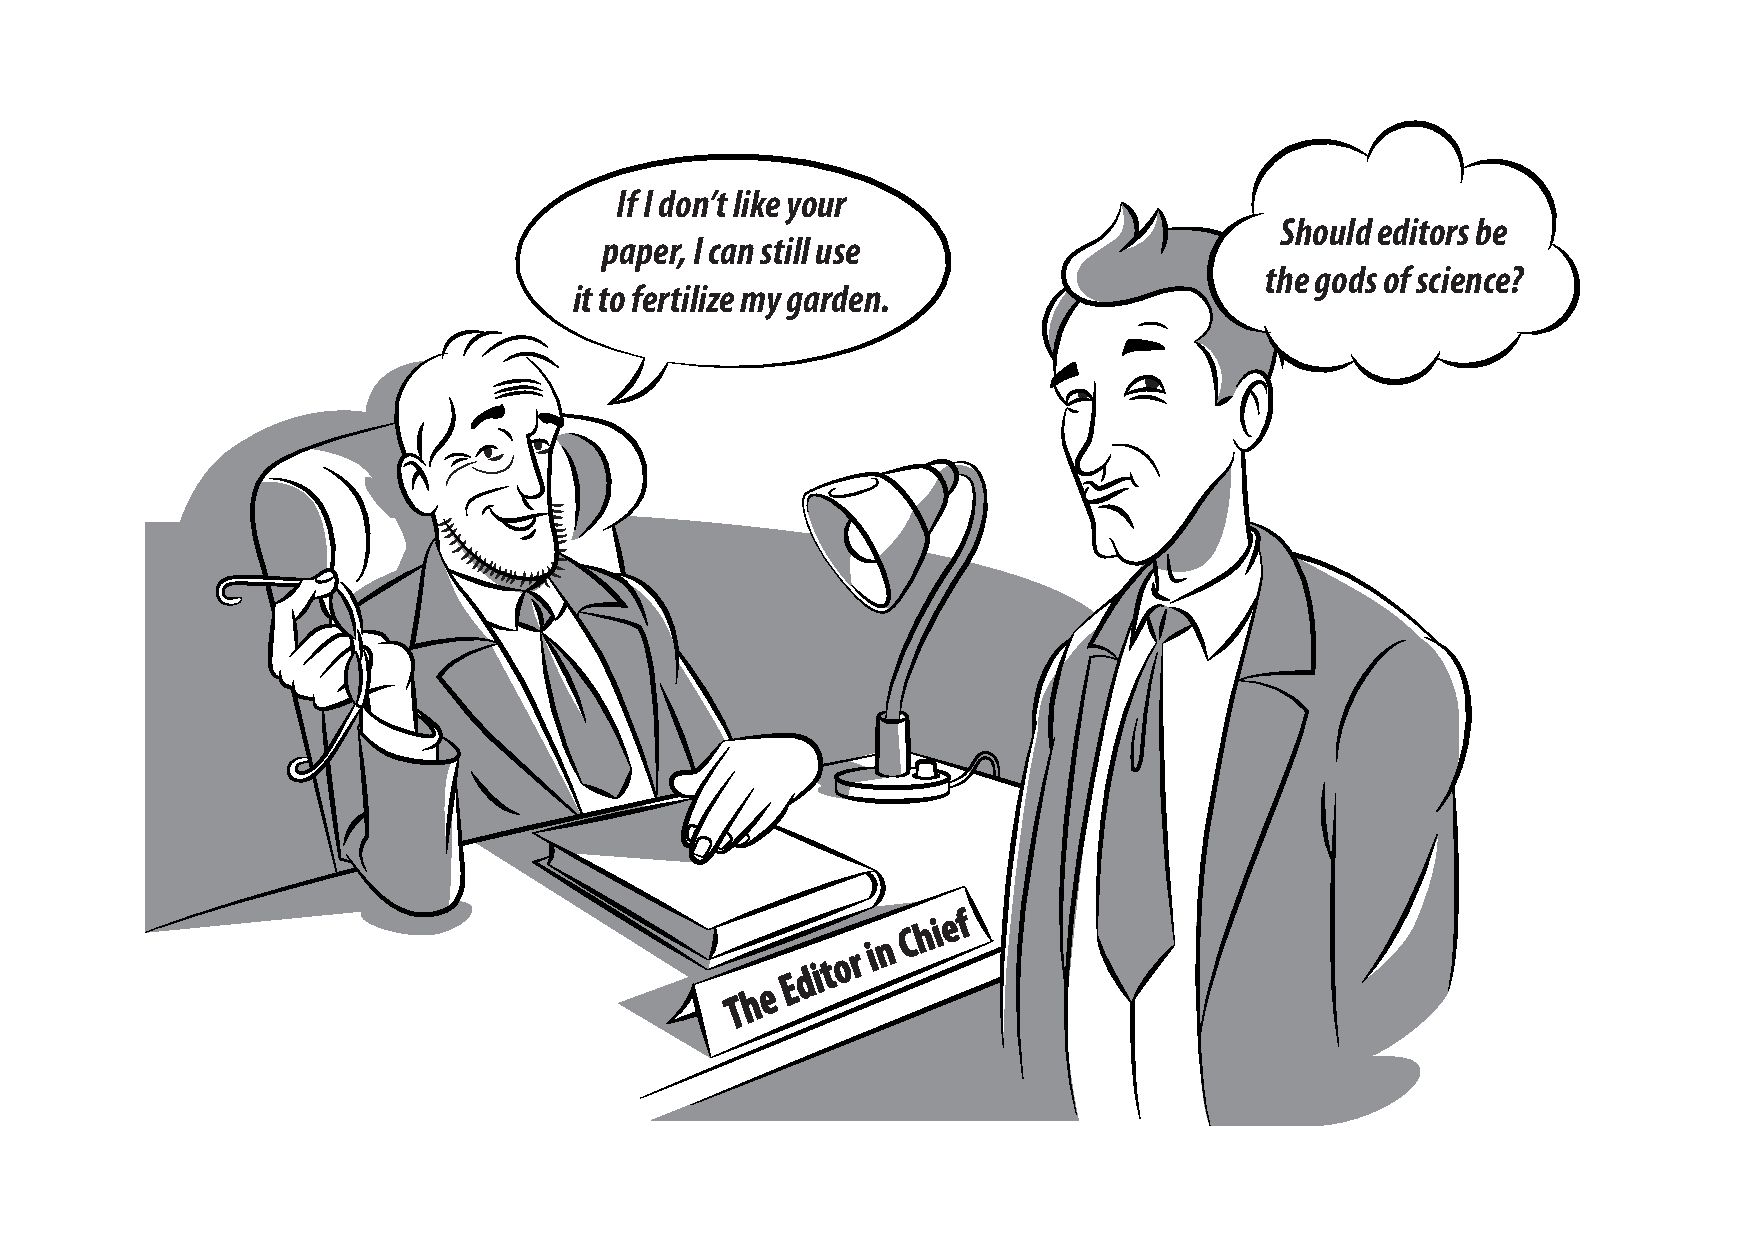
\includegraphics{Fig_editor.pdf}}
\end{center}

Editors usually have the last word in an editorial system. Often, they do not need to justify their actions or decisions to anybody. One of the biggest paradoxes is that the first rule of science rejects the very idea of authority, yet journal editors get exclusive rights to shape science.\par

The American Physical Society\index{American Physical Society} has published a number of ethical guidelines\footnote{\url{http://www.aps.org/policy/statements/}} that define a culture --- the \emph{`code of honor'}\index{code of honor} of scientific publishing. The most important points from this code, according to \citet[p.129-32]{AscheronKickuth2004} are:

\begin{itemize}\renewcommand{\labelitemi}{$\checkmark$}
  \item \emph{Publish substantial and new results only. Avoid re-publication.}
  \item \emph{Do not falsify or invent data.}
  \item \emph{Avoid plagiarism, respect copyright.}\index{plagiarism}
  \item \emph{Limit the list of authors to people who were actually involved.}
  \item \emph{Share responsibility/merit with the co-authors (make everybody read and write the paper).}
\end{itemize}

If you suspect problems with scientific integrity such as fraud, plagiarism, infringement of copyright, incomplete information or improper pressure from superiors or contract partners, you should first try to contact people within your institute --- a department head and/or professional member of staff such as a research advisor --- for advice. If this doesn't work, you might consider submitting an objection via the publisher's website (look under \emph{``Report This Content''}) and/or by contacting an international organization such as COPE. \par

\begin{svgraybox}
Is someone who just signs bills an author? They shouldn't be. The author of an article must be someone who contributed to the intellectual content of a manuscript by participating in the design of an experiment, in data processing, or in writing and/or editing the article.
\end{svgraybox}\label{R:authors}

The author of an article should only be someone who participated (physically and/or mentally) either in:
\begin{enumerate}
 \item field/laboratory data collection, and/or
 \item data processing and statistical analysis, and/or
 \item writing and editing the paper.
\end{enumerate}

If someone is listed as a co-author, this means that he/she made a significant contribution to the intellectual content of the manuscript. A research investigation is not routine work. Hence, a laboratory technician should not become a co-author of the article simply for carrying out routine laboratory analysis that he/she conducts on a regular basis. A co-author of an article should have invested own creativity and original ideas/data. Our experience is that the principal author is usually responsible for producing about one to two thirds of the paper, while the co-authors mostly get involved in the final phases of production. So, if your supervisor, head of project or other superior asks for their name to be listed on the paper, there is still some time for them to get involved. However, if they ask for their name to be automatically listed on the paper without any serious involvement, this is wrong and immoral.\par

The artificial pressure to publish, with all of its negative side-effects, can be simply avoided by introducing more sophisticated evaluation criteria. Quality is much more important than quantity\footnote{However, Google derives most of its profit from the brilliant idea of listing sites by the number of times they have been accessed. Quantity sometimes determines quality.}. Having your name on 20 \emph{born-dead} SCI papers cannot be more important than publishing a single high-impact paper. In fact, in many countries, scientific evaluation teams do not even distinguish between the first and last author.\par


 \section{Missing reviewers}\label{sec:missingreviewers}

Reviewers (referees) are crucial for the quality of scientific information. Because reviewers are typically not rewarded or even mentioned for their work, they often deliver a slow or poor service. In fact, reviewers are asked to do high-quality consultancy without any compensation. You could argue that they do benefit by getting early access to papers from colleagues (plus the discipline of reviewing makes them read such papers carefully,which they don't always do otherwise), but the fact is that their work is not directly rewarded.\par

In an optimal situation, a reviewer will take one day to read the paper and then a few days to cross-check its findings. Such an investment of time is clearly a luxury that few can afford, so reviews are usually done in a few hours. In fact, because the volume of papers published is continually increasing, there is less and less time for proper reviews. Many good reviewers refuse review assignments because they are overloaded with writing papers, or they agree to do reviews which are incomplete or superficial \citep{Newmark2003Nature,Moore2005CSAN}. Also, reviewers sometimes grade and comment only on the form and style of a paper and not on its intellectual content. \par

Fiona Godlee, editor in chief of the BMJ Group thinks that \emph{``scientists are under a lot of pressure on a whole host of things --- getting funding and the bureaucracy surrounding scientific research --- and peer review is just one other thing, so the more we can do to make it something that they can gain proper recognition for, the better.''} \citep{ODowd2011}.\par

\begin{svgraybox}
A major problem for many scientific journals is the review process, which is often slow, inefficient, inconsistent, unrepresentative and biased. This is because reviewers are not rewarded for their work or evaluated on their performance. One solution to this problem would be to completely open up the review process and publish both the signed results of reviews and the authors' responses, together with all versions of a paper (\emph{``Open Peer Review''})\index{Open Peer Review}, so that both authors and reviewers can be properly acknowledged for their work.
\end{svgraybox}\label{R:editors}

Most journals allow 1--6 months for the return of reviews, which does not mean that the reviewers spend that much time reading and thinking about the papers. Unfortunately, when a paper lands on a reviewer's desk, it will first gather dust for some time. Eventually, the reviewer will find time to read it and make comments (usually taking half a day). Often the editor needs to find a replacement for the reviewer because he/she does not respond. Because reviewers are not rewarded for their work, they may find it difficult to justify this investment in time to their employers. Many companies, even government organizations, do not like the fact that their staff spend paid time on reviewing papers, for which only the publisher receives financial benefit.\par

In the worst-case scenario, reviewers sit on a paper or give it a bad review because it is in their interest. The editor or publisher typically cannot complain because they are not paying for this work. As a result, reviewers often do not feel responsible for their output.\par


\begin{figure*}[htb]
\begin{center}
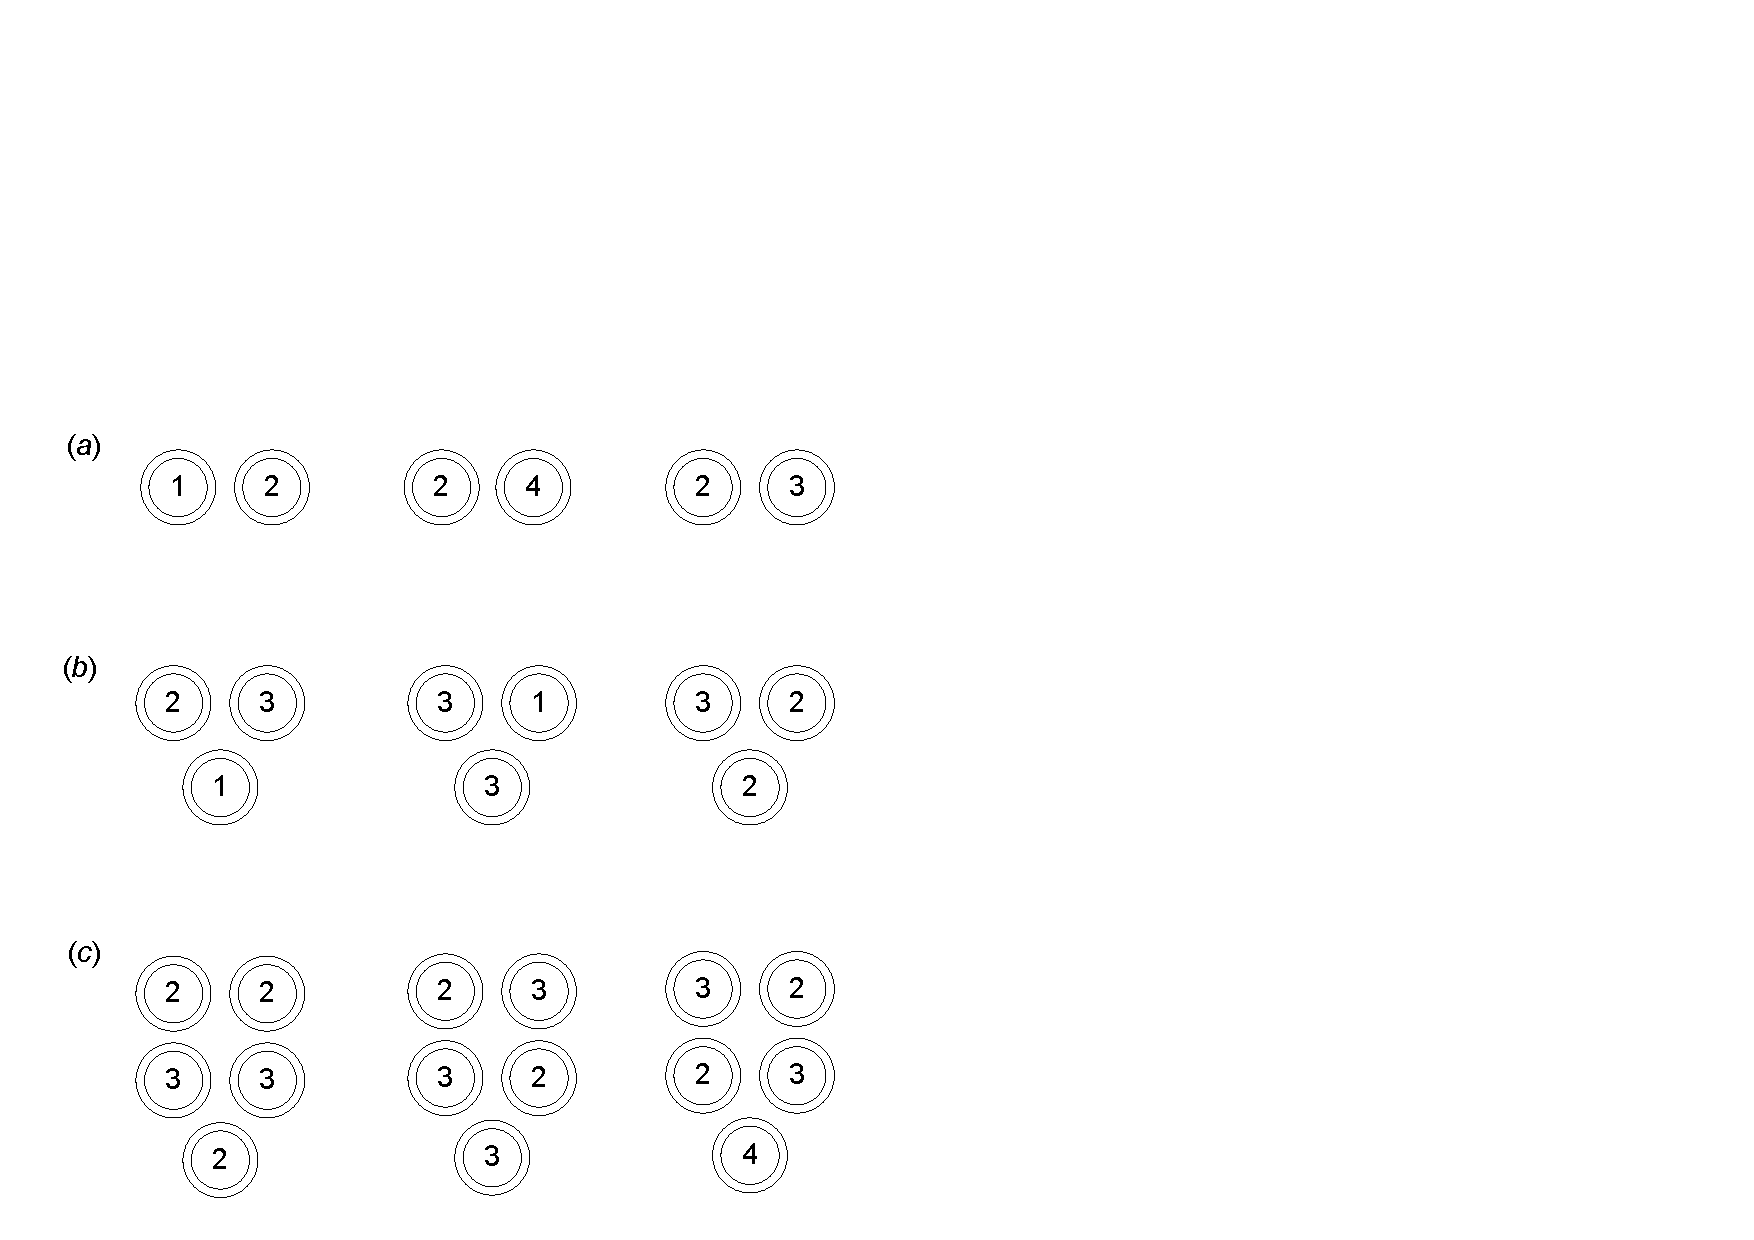
\includegraphics[width=.8\textwidth]{Fig_review_sim.pdf}
\caption{Three simulations of reviewers' decision with different samples. Deciding on an average from a sample of two can lead to some strange outcomes (a). Three is slightly better, but still difficult (b). With five samples (c) we can be probably be more confident. ``1'' --- accepted with minor revision; ``2'' --- accepted with moderate revision; ``3'' --- major revisions needed and ``4'' --- rejected.}
\label{F:sim}
\end{center}
\end{figure*}

In most cases, an editor will be happy with just two completed review forms. It can easily be shown that a decision based on only two or three reviews can lead to fairly poor estimates. In fact, two reviews often contradict each other. Consider a Monte-Carlo simulations of review decisions with different sample sizes. In this example there are four grades for papers: (``1'') accepted with minor revision, (``2'') accepted with moderate revision, (``3'') major revisions needed and (``4'') rejected. Now imagine that the grades are based on negative points (0--100), where papers with $<10$ negative points are classified as ``1'', $<40$ as ``2'', $<70$ as ``3'', while the papers with $\geq 70$ points are rejected.\par

Fig.\@~\ref{F:sim} shows the results of the Monte-Carlo simulations using $x$=40, $s_x$=20 and 2, 3 and 5 for sample size. Note that in the case of only two samples, the decisions can vary from accepted with moderate changes to rejection (Fig.\@~\ref{F:sim}a). We estimated that, if a sample of two is used, in about 30-50\% of cases the decision will differ from the expected one. The situation is a little better for the sample of three (only 30--40\%) and much better if a sample of five is used ($<20$\%). The results of this simulation exercise, of course, depend on how variable the opinion of the reviewers is, but we hope we have illustrated the problem. \par

A number of studies have been published over the years showing that there is often little agreement among independent referees about whether or not a paper should be published \citep{schultz2010Scientometrics}. The major issues connected with why some decisions are positive and some are negative are: confidentiality, conflicts of interest, editorial freedom and integrity, the lack of uniformity of the review process, etc.\par

The current problems with poor or delayed reviews could be avoided by rewarding reviewers for their work. This need not necessarily be a financial reward. It would be enough for journals to list reviewers and the amount of work they have done. In fact, editors could monitor how satisfied authors are with the work of reviewers and then, based on certain criteria, promote successful reviewers to become senior reviewers (or at least give them some kind of diploma or symbolic reward). Reviewers could then add such information to their resum\'{e}s and use it to get greater acknowledgment in their research community. Another (cheap) solution to the problem of biased and unrepresentative reviews would be to ask all members of a society to participate in the review of all papers. This could be organized through on-line editorial systems, in which all reviewers can (at any moment) see the results of the reviews and jointly grade the intellectual and technical quality of an article. \par

\bigskip
\begin{fminipage}{.9\textwidth}{\footnotesize{\textsf{\textbf{On Scholarpedia}}\index{Scholarpedia}: Scholarpedia is the peer-reviewed open-access journal for \emph{living review}-type articles: \emph{``The goal of Scholarpedia is to identify and convince today's Einsteins and Freuds to write encyclopedia articles on their fundamental discoveries so that 100 years from now the best experts will be willing to maintain and update the articles through the process of curatorship.''} Scholarpedia articles can be cited and are constantly updated by their curators with contributions by registered members. The job of a curator is to moderate revisions of an article (accept/reject). To publish an article on Scholarpedia you need to get two existing curators to write to the editor-in-chief, and then keep maintaining it.} }
\end{fminipage}
\bigskip

Scientific journals, in general, could learn a great deal from \textsc{Wikipedia}\index{Wikipedia@\textsc{Wikipedia}} --- the Open Encyclopedia --- and the journal version of \textsc{Wikipedia} --- Scholarpedia\footnote{\url{http://scholarpedia.org}} (see box). In \textsc{Wikipedia}, every registered member can at any time edit a topic and see the history of edits and search edits\footnote{\url{http://en.wikipedia.org/wiki/Wikipedia:Five_pillars}.}. This saves reviewers a lot of time because they don't need to repeat work, but it also saves the authors time, because they get feedback much faster. \par

Another way to improve the review process is to reward the reviewers with discounts and/or to assign them some kind of priority status \citep{Newmark2003Nature}. For example, journals published by Berkeley Electronic Press\footnote{\url{http://www.bepress.com}} have introduced an innovative concept in which they do not charge submitting authors if they contract to provide a timely review of an agreed number of articles. The authors are charged if they fail to deliver their reviews on time, which seems to be a pretty fair system. Likewise, Scholarpedia ranks authors who contribute to articles so that, once the curatorship of an article becomes vacant, it is automatically offered to the reviewer with the highest index for that article. \par


\section{Fashionable pliability}

\begin{quote}
    \emph{``What makes things hard to understand is how complicated they are, not how big they are.''}\footnote{Martin Rees in \emph{``Our Final Century''}.}
\end{quote}

The final serious problem with the current system of science is the ease with which authors follow fashionable topics or styles. On the one hand, it is positive to learn from top researchers. On the other, those who imitate other authors forget that in science we need to be cautious and critical about everything. Some authors see their supervisors as Gods of science and blandly repeat whatever they say or write. Their identity is thus lost and they become eternal second authors. Other authors think that, if they choose a sufficiently \emph{`sexy'} topic, this will guarantee them success in getting their papers published (which is often unfortunately true). \par

To prove that there is a lot of gibberish being published in science today, three MIT students submitted an abstract entitled \emph{``Rooter: a methodology for the typical unification of access points and redundancy''} to the World Multi-Conference on Systemics, Cybernetics and Informatics in 2005. The abstract was accepted for oral presentation and printed and nobody would have complained if the authors had not admitted that they produced this abstract using a computer program\footnote{At \url{http://pdos.csail.mit.edu/scigen/} you can generate a nonsense paper yourself.}\index{nonsense paper, generator} that randomly incorporated computer science jargon and produced a grammatically correct yet nonsensical paper (see New Scientist magazine, issue 2496).\par

A more extreme example is that of Alan Sokal who, in the late 1990s, managed to publish a totally nonsensical paper in a respected journal. Alan Sokal (a Professor of Physics at NYU), succeeded in getting a text advancing critiques of science and rationality common in certain academic disciplines published in a cultural studies journal. Sokal wrote a parody of post-modern science criticism called \emph{``Transgressing the boundaries: towards a transformative hermeneutics of quantum gravity?''}. This was submitted to the cultural studies journal Social Text, without telling the editors that it was a parody. They published it as a serious scholarly article and, when the author revealed the hoax three weeks later, people were very angry with him. Like the genre it was meant to satirize, the article was a mixture of truths, half-truths, falsehoods, non sequiturs and syntactically correct, high-flown language that had no meaning whatsoever. It also contained appeals to authority rather than logic, rhetoric that sounds good but whose meaning was ambiguous, and confusion between the technical and everyday senses of English words (for example, linear, non-linear, local, global, multidimensional, relative, frame of reference, field, anomaly, chaos, catastrophe, logic, irrational, imaginary, complex, real, equality and choice). The article was riddled with significant stupidities and falsities concerning science, which the editors missed.\par

By doing this, Sokal was trying to suggest that in those milieus, some people had virtually no knowledge of the science they were so blithely critiquing. You can read more on the topic in \citet{SokalBricmont1997} and \citet{Sokal1998S}. Below is a similar example taken from an original passage (pp.~44-45 and a footnote on pp.~327-328) in \emph{A Short Course in Intellectual Self-Defense} by Normand Baillargeon  \citep{Baillargeon2008short}: \par


\bigskip
\begin{fminipage}{.9\textwidth}{\footnotesize{\textsf{\textbf{The Fox Hypothesis}}\index{Fox Hypothesis}: Those who pulled off the hoax, which brings to mind Sokal's at the end of the 1990s, formulated what they called the Fox hypothesis, according to which an unintelligible speech, if given by a seemingly legitimate source, will tend to be accepted as intelligible. A corollary of this idea is that using vocabulary that creates the illusion of profundity and erudition can contribute to increasing the credibility of a message. At the beginning of the 1970s, Dr.\@ Fox gave a talk on three different occasions, entitled \emph{``Mathematical Theory of Games and its Application in the Training of Doctors''}. He spoke in front of a total of fifty-five people, all highly educated: social workers, educators, administrators, psychologists, and psychiatrists. His exposition lasted an hour and was followed by a half-hour-long discussion. Then a questionnaire was distributed to the audience to find out what those present thought of the doctor's presentation. All the participants found it clear and stimulating; none of them noticed that the talk was total nonsense, which it was. Dr.\@ Fox was actually an actor. He looked very distinguished and spoke authoritatively and with conviction. But the text he spoke, which he had learned by heart and which had to do with a topic he knew absolutely nothing about, was laden with vague words, contradictions, bogus references to concepts that had nothing to do with the topic, empty concepts, and so on. In short, it was nothing but hot air, contradictions, and pompous meaninglessness.} }
\end{fminipage}
\bigskip

Young academics and, especially non-native speakers, assume that the best way to get published is to imitate the heavy, unreadable articles they see in many journals and textbooks. Such beliefs are based on a big misunderstanding. What actually gets articles published in top journals and more importantly read, is clear, well-structured, well-argued writing. One underlying issue is that we learn to write in an artificial context, showing teachers and professors what we --- and they --- already know. We therefore tend not to formulate clear arguments when addressing real-world readers, where the goal is to persuade an audience of the validity of a new solution to a serious problem.\par

Another common misconception among researchers is that their ultimate career move would be to publish in Nature, Science or a similar journal with a high impact factor. This is a rather naive conception, which is nicely demonstrated by \citet{Seglen1997BMJ}. The correlation between a journal's impact and the actual citation rate of articles from individual scientists or research groups is often poor (Fig.\@~\ref{Fig:JIF_vs_RAI}). In fact, publication in a high-impact journal will not necessarily increase the impact of an article \citep{Seglen1997BMJ}. Therefore, you should focus on writing high-quality articles and not on trying to get into top journals at any cost.\par


\section{Publishing companies and models}\label{sec:publishing_models}

\begin{quote}
    \emph{``Who are the most ruthless capitalists in the Western world? Whose monopolistic practices makes WalMart look like a corner shop and Rupert Murdoch look like a socialist? You won't guess the answer in a month of Sundays. While there are plenty of candidates, my vote goes not to the banks, the oil companies or the health insurers, but --- wait for it --- to academic publishers.''}\footnote{Article by George Monbiot. Published in the Guardian 30th August 2011}
\end{quote}


In his review of the current copyright policies in the world, the author and director of the documentary Remix Manifesto, Brett Gaylor, warns us of the increasing risk of corporations taking over control of human culture. For the large corporations ideas are intellectual property that, like any other product, can be commercially exploited to make a profit. Large media corporations are becoming increasingly powerful. In the USA, companies such as Disney, TimeWarner, Viacom, NewsCorp, BMG, and General Electric now own $>$90\% of media holdings. Such large corporations use political lobbies --- and their financial strength --- to impose more and more control over ideas. \emph{``Patents, innovations and corporate secrets are now guarded like gold.''} Companies today try to copyright everything --- even broad ideas and legacy information that used to be available in the public domain.\par

If you extrapolate these trends, it is possible that in some 20--30 years large companies might come to own and control most of human knowledge and thus attempt to completely lock up human culture\footnote{As Lessig warns us in his book \emph{``Free Culture''}: \emph{``copies in our brain are not --- YET --- regulated by copyright law.''}}. Gaylor emphasizes that the public domain needs to be protected and that the control that commercial companies currently have needs to be limited to ensure the continued free exchange of ideas. He builds his argument on the following four premises:\index{copyright}\index{Lessig}

\begin{itemize}
  \item Culture builds on the past
  \item The past always try to control the future
  \item Our future is becoming less free
  \item To build free societies you must limit the control of the past.
\end{itemize}

Or as Lawrence Lessig puts it in \emph{``Free Culture''}\index{Free Culture}: \emph{``Overregulation gives dinosaurs a veto over the future; it wastes the extraordinary opportunity for democratic creativity that digital technology enables.''}\par

Something similar can be said for scientific publishing. The best-known traditional \textbf{Science, Technical and Medical} (STM) publishers\index{publishing!commercial companies} are companies such as Elsevier, Wiley, Springer, and Taylor \& Francis, which have a long tradition and often an international network of employees. These companies hold $>$50\% of the global market of STM publishing, which is estimated as between 7 and 11 billion US\$ \citep{ICU2006}. For more than 200 years the STM publishing companies have been sharing access to scientific information and have made profits via the system of copyright ownership \citep{Collins2005JACR}. The market leader, Reed Elsevier\index{Elsevier}, makes nearly 40\% of all its profits from the journal business and this profit is significant\footnote{The financial reports are available at \url{http://reports.reedelsevier.com}.}.\par

The standard publishing model used by the traditional STM publishers is described in Table~\ref{Tbl:publishing_models_comparison}. It can be summarized as follows: companies establish copyright over scientific articles in order to ensure financial benefits and they keep the review processes closed to protect their role. Science is then restricted to those who can afford it. More than two thirds of the world's population live in countries that are recipients of Official Development Assistance\footnote{\url{http://www.oecd.org/dac/stats/daclist}} (ODA). Most people in these countries have no access to \emph{state-of-the-art} scientific literature \footnote{Thanks to initiatives such as \url{ahttp://www.research4life.org}, developing countries also have a chance to access research publications at low cost.}, which means that the gap between the rich and the poor is likely to continue growing. It is not that the commercial STM publishers are responsible for this inequality --- they just perpetuate it. If you don't think that this gap is as serious, just try doing science for few months in a country where you can't access most of the recent literature in your field. \par

\begin{table}[!hbt]\index{Open Publishing}
\centering \caption{A comparison between the traditional and the Open Publishing  models.}\label{Tbl:publishing_models_comparison}
\setlength{\extrarowheight}{8pt}
\begin{tabular}{m{.32\textwidth}m{.32\textwidth}m{.32\textwidth}}
\toprule
 & \parbox[c]{.32\textwidth}{\centering Traditional STM \par publishers} & \parbox[c]{.32\textwidth}{\centering Open Publishing \par model } \\
\midrule
 Copyright held by & \parbox[c]{.32\textwidth}{\centering company} & \parbox[c]{.32\textwidth}{\centering author(s) of \par the article} \\
 Publication costs \par (Open Access) & \parbox[c]{.32\textwidth}{\centering typically in the range \par 1500--3000~US\$} & \parbox[c]{.32\textwidth}{\centering from completely sponsored \par to 1500~US\$} \\
 Specification of costs \par in the bill & \parbox[c]{.32\textwidth}{\centering $\times$} & \parbox[c]{.32\textwidth}{\centering $\checkmark$ } \\
 Time delay from submission \par to publication & \parbox[c]{.32\textwidth}{\centering typically in the range \par 3--12 months} & \parbox[c]{.32\textwidth}{\centering usually minimized \par (immediate publication)} \\
 Line editing and \par technical support & \parbox[c]{.32\textwidth}{\centering typically left to authors \par to organize} & \parbox[c]{.32\textwidth}{\centering on request} \\
 Access to pre-publication \par history & \parbox[c]{.32\textwidth}{\centering $\times$} & \parbox[c]{.32\textwidth}{\centering $\checkmark$ } \\
 Signed reviews  & \parbox[c]{.32\textwidth}{\centering $\times$ } & \parbox[c]{.32\textwidth}{\centering $\checkmark$ } \\
 Live support & \parbox[c]{.32\textwidth}{\centering $\times$ } & \parbox[c]{.32\textwidth}{\centering on-line status of editors \par and reviewers visible} \\
Post-publication editing \par (corrections / errata) & \parbox[c]{.32\textwidth}{\centering 48--hour period \par for page-proofs} & \parbox[c]{.32\textwidth}{\centering corrections also possible \par even after publication} \\
 Involvement in the activities of research groups  & \parbox[c]{.32\textwidth}{\centering limited } & \parbox[c]{.32\textwidth}{\centering the publisher also organizes \par conferences and workshops} \\
\bottomrule
\end{tabular}
\end{table}

Publishing reached a totally new level with the launch of the Internet some 20 years ago. \emph{``Before the Internet, it was inconvenient to retrieve an article that was not available in a local library system. Now it is inconvenient to go to a library''} \citep{Collins2005JACR}. Almost all STM publishing companies have switched to \emph{digital publishing}, which means that most of their products are available on-line as digital media (PDF) and are stored in a database. Big commercial companies, of course, see digital publishing primarily as a new source of profit. But, thanks to the revolution of Internet and a great deal of enthusiasm, some new models are starting to take off: Open Access publishing and Open Access archiving\footnote{To find out more about the Open Access movement, see e.g.\@ Peter Suber's website at \url{http://www.earlham.edu/~peters/fos/}, and/or read the Berlin declaration on Open Access.}.\par

Table~\ref{Tbl:publishing_models_comparison} shows the characteristics of what we call the \emph{``Open publishing model''} --- a model in which articles are immediately published in their original form and made freely available to anyone. In this model reviewers take responsibility for their work, and review --- i.e.\@ the pre-publication history --- is transparent. Authors keep their copyright and the publisher is closely linked with the research societies connected with the journal. \par

Is Open Publishing an utopia? Commercial companies have criticized Open Access publishing for not being realistic about their OA author costs. \citet{Regazzi2004SR}, the managing director at Elsevier, thinks that the author fees of BioMed Central and/or PLoS are insufficient to cover the actual publishing costs. He believes these costs are likely to be the same as those of any traditional publisher, but the final price is lower because the costs are either subsidized and/or the OA publishers underestimate the true costs of sustainable publishing. He thinks OA journals are no threat to commercial publishers, because (1) they are insignificant and (2) they do not really innovate in publishing. \emph{``Open Access or author-pays publishing solves neither the problem of easy access to scientific information nor the innovation funding problem --- OA publishing will neither decrease publishing costs, nor can it generate enough capital to invest in the future development of increased access''} \citep{Regazzi2004SR}\index{Open Access!author-pays}.\par

To explore this issue, we can ask whether it is possible to publish quality OA journal articles and books without paying author fees at all. There are few examples, but there are some. The Journal of Statistical Software (JSS, published by the American Statistical Association), for example, is an OA journal that is indexed in Science Citation Index Expanded and its impact factor is increasing (${\rm JIF}$ = 2.3 in 2009). What is really interesting about this journal is that there is no charge for submission and no charge for subscription. It gets even better: for both articles and code snippets JSS publishes the source code along with the paper. How do they do it? First, they have minimum costs because they exclusively use Free and Open Source packages ({\LaTeX}\index{Free and Open Source Software!\LaTeX} for typesetting and Ruby on Rails\index{software!\textsf{Ruby on Rails}} for website Content Management System\index{Content Management System}). Second, they distribute only electronic versions of papers, so there are no printing costs\footnote{Books are also increasingly published as OA materials. A number of \emph{``Free''} books can be found at \url{http://www.gnu.org/doc/other-free-books.html}.}.\par

\begin{svgraybox}
Open Access journals are no different from traditional subscription-based journals --- they undergo the same peer-review and quality control as any other scholarly journal. The main difference is that with OA journals: (1) you typically maintain copyright, which means that you can share your knowledge freely, (2) the whole publishing process is usually more transparent.
\end{svgraybox}\label{R:OA}

This book is published via Lulu.com\index{Lulu} --- one of the biggest self-publishing companies in the world. There were NO submission costs for publishing this book at Lulu and we have kept our copyright and revision rights. We could check the price of a single copy long before sending the book to the publisher. Hence OA, either with low submission fees or through sponsored publishing is possible. The question is: how can we make it the mainstream publishing model of the future?\par

The best-known primarily OA publishers in the world are currently:

\begin{itemize}
  \item \textbf{Public Library of Science (PLoS)}\index{Public Library of Science} --- PLoS is a nonprofit organization of scientists and physicians that publishes articles in biology, medicine, genetics, computational biology and related fields. The OA costs per article are in the range of 1500-2000~US\$, depending on the journal. These costs are lower than those of STM publishers, partly because PLoS has received millions of dollars of charitable support.
  \item \textbf{BioMed Central (BMC)}\index{BioMed Central} --- BMC (now owned by Springer) currently charges between 500 and 1750~US\$ per article.
  \item \textbf{Hindawi Publishing Corporation}\index{Hindawi} --- Founded in 1997 and based in Egypt, Hindawi maintains 200+ journals in various fields from Agriculture to Physics and Neuroscience. It has a large number of editors spread around the globe.
  \item \textbf{Copernicus Publications}\index{Copernicus} --- Copernicus maintains some 40+ journals, primarily for the Earth sciences and geosciences.
  \item \textbf{Molecular Diversity Preservation International (MDPI) Publishing}\index{MDPI} --- MDPI is an organization for the deposit and exchange of molecular and biomolecular samples located in Basel, Switzerland. Established in 1996, it hosts some 40+ Open Access journals, mainly in the field of molecular biology and bio-sciences.
  \item \emph{Other specialized OA publishers\footnote{For a complete list see: \url{http://www.doaj.org}.}}\index{DOAJ}\index{Open Access journals} --- In the USA and Europe there are now several scholarly publishing houses that can completely accommodate OA publishing. For example, the American Meteorological Society and the Institute of Electrical and Electronics Engineers.
\end{itemize}

OA is slowly becoming accepted by both commercial and academic publishers. Even commercial publishers have recognized the potential of OA publishing and its ethical logic. The main barrier is still conservatism among authors and publishers alike. OA is also often misunderstand. To clarify the main principles of OA, BioMed Central, one of the leading Open Access publishers has published a lengthly response to the most prevalent anti-open-access arguments --- Misleading Open Access Myths\footnote{\url{http://www.biomedcentral.org/openaccess}}. \par

There are also two moral dilemmas in the current toll-access publishing system. First, science should not be a luxury that's restricted to an elite. Second, why should we have to pay for the results of research that is funded by public money? As \citet{Kleiner2011} puts it: \emph{``If the public is funding the research, the public should be able to see it.''} \par

\bigskip
\begin{fminipage}{.9\textwidth}{\footnotesize{\textsf{\textbf{On self-publishing}}\index{self-publishing}\index{publishing!self-publishing}:
Self-publishing is publishing outside formal organizations i.e.\@ without professional publishers. The main problem with it is that it often leads to \emph{`gray'} literature\index{gray literature}. This is the type of literature that lacks strict bibliographic control or professional layout and can therefore disappear in a few years. Self-publishing typically means low-budget production, because individual authors start with limited resources. Another problem is that self-publishing suggests that the authors do not appreciate the opinion of the research community or that the work is unchecked. The whole idea of peer review is that other people read someone's work and then give feedback and evaluate it. However, as we argue elsewhere in this book (page~\pageref{sec:missingreviewers}), the peer review system is in urgent need of drastic overhaul. Hence most publications in STM journals are also the result of self-publishing in a way --- journal editors do not try to improve or help redesign articles, but are primarily interested in their ranking (i.e.\@ minimum potential negative publicity). Most peer reviewed (commercial) scientific publications express only the opinions of authors, are often poorly checked, and come with no warranty. } }
\end{fminipage}
\bigskip

Self-publishing should not present science with any problems as long as the values are right. \citet[p.85]{rees2004our} agrees that \emph{``any potentially epochal claim, provided it is openly announced, will be guaranteed to attract wide scrutiny from the international community of experts. So it doesn't matter a great deal if formal review is bypassed, provided that there is no impediment to openness.''} In other words: open publishing is probably more important to science than peer review.\par

Many large STM publishers now provide an OA option by charging authors either a fixed amount or an estimate that is based on average costs\footnote{See \url{http://www.sherpa.ac.uk/romeo/PaidOA.html}.}. Elsevier, for example, charges about 3000~US\$ for open access. A number of institutions\footnote{\url{http://www.elsevier.com/fundingbodies}} have signed a special agreement with Elsevier to meet the OA fees on behalf of their authors. Springer has started a user-friendly service for Open Access publications called \emph{``Open Choice''}\footnote{\url{http://www.springer.com/openchoice}}. The idea behind this is to simplify OA publishing: Springer signs agreements with universities and libraries, so that the bill for OA goes to the organization and not to individual authors. This \emph{``green road''} to OA publishing may well represent the best business model to follow until the wider scientific community comes to accept the logic of OA. Springer also hosts a number of Open Access journals\footnote{\url{http://www.springeropen.com/journals}}, and is currently the leading STM company in the field of OA.\par

\citet{WellcomeTrust2004} has estimated that the costs for a good-to-high-quality OA article would be about 2000~US\$. Their report further recognizes that \emph{``an author-pays system has the potential to be more economically efficient, both in terms of the allocation of resources between competing uses and in the level of total system costs.''} It is likely that the provision of open, electronic archives will effectively create an open access system for readers \emph{``which could fatally damage subscriber-pays systems in the long term''} \citep{WellcomeTrust2004}. While the pros and cons of OA publishing are still being debated, we believe there are no valid arguments against OA archiving (see next page), especially when you think of the benefits it brings to developing countries. \citet{Evans2009Science} discovered that, in developing countries, free-access articles are much more likely to be cited and are likely to make more impact than articles in commercial journals. \par

\bigskip
\begin{fminipage}{.9\textwidth}{\footnotesize{\textsf{\textbf{Internet and its side-effects}}\index{internet!growth rates} --- Internet is considered to be one of the most promising prospects for humanity \citep{Glenn2009}. The advent of worldwide, decentralized communication epitomized by the internet and cell phones has been a pervasive democratizing force \citep{Kurzweil2005}. Think of the role they have played in the popular revolutions in Tunisia, Egypt, Yemen and Syria. Nearly 25\% of humanity is already connected to the internet. If one extrapolates current internet growth trends (internet traffic growth doubles every 6 months; bits/dollar efficiency doubles every 12 months; the internet router/switch max speed doubles every 6 months), then it is easy to see that in 5--10 years almost everyone will have efficient, inexpensive access (Fig.\@~\ref{Fig:internet_plots}). In such a future, open access to science should not cost a fortune (as the commercial publishers argue right now).
}}
\end{fminipage}
\bigskip

Another good example of an OA publisher that supports open publishing is \textbf{Copernicus}\footnote{\url{http://publications.copernicus.org}}\index{Copernicus}, a not-for-profit publishing corporation closely linked to the European Geosciences Union (EGU). The model that Copernicus uses is truly innovative. First, submitted papers are immediately published as discussion papers, which means that there is no delay between submission and publication of research results. Second, reviewer's reports, authors' responses and any other comments --- which anyone can submit, whether anonymously or with contact details --- are also published immediately. Third, Copernicus is closely involved in the organization of conferences and similar events for the EGU. Copernicus charges various author fees, depending on the journal, which are fully specified in the bill sent to authors. \par

The following five practical advantages of OA publication are worth mentioning:

\begin{enumerate}\renewcommand{\labelenumi}{(\textit{\alph{enumi}})}
  \item \emph{You allow open access to your work},
  \item \emph{Your article is immediately available on-line},
  \item \emph{You own the copyright for your work},
  \item \emph{You can track who is reading your paper and when},
  \item \emph{You can print out as many copies of your article as you need and e-mail copies to anyone you like}.
\end{enumerate}



\begin{figure*}[!htb]
\begin{center}
  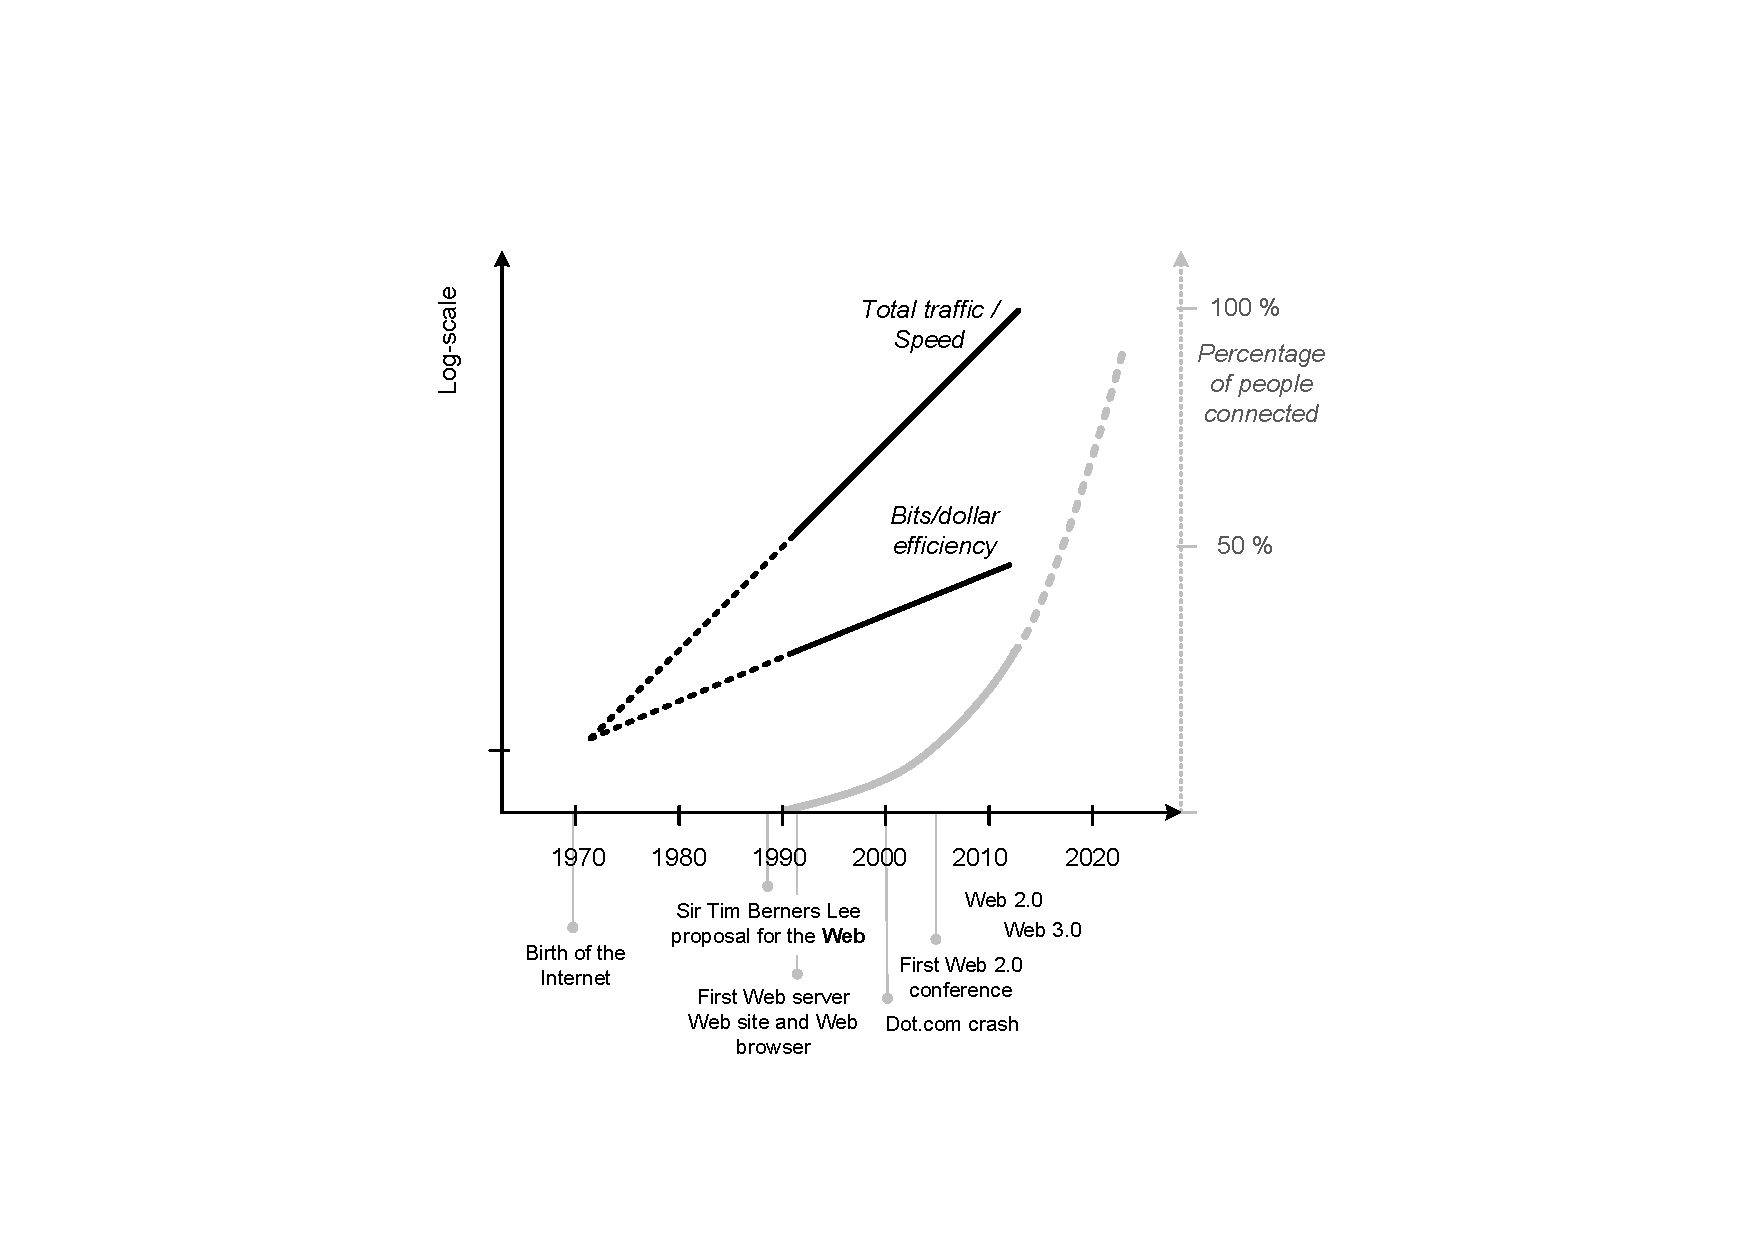
\includegraphics[width=.8\textwidth]{Fig_internet_plots.pdf}
\caption{Evolution of the internet follows an exponential growth curve. There is every reason to expect that in the 5--10 years almost everyone will have efficient inexpensive access.} \label{Fig:internet_plots}
\end{center}
\end{figure*}

Finally, articles can easily be made accessible to the scientific community through \textbf{open access archiving}\label{sec:OAA}\index{Open Access!archiving}, by interlinking repositories of publications or by publishing OA digital copies after an agreed period of time. The UK Government Select Committee Report on Science Publishing\footnote{Recommendations published at \url{http://epublishingtrust.org}.} says: \emph{``We recommend that the Research Councils and other official funding organizations mandate their funded researchers to deposit a copy of their articles in their institution's repository within one month of publication{\ldots} as a condition of their grant,''} and the US government has recommended that research funded by the National Institutes of Health be likewise archived. Archiving already published research in interoperable institutional archives greatly benefits global science at virtually zero cost. This can be done now, without changing established publishing practices \citep{ICU2006}. For developing countries this creates enormous opportunities, especially in agricultural and medical research\footnote{Steven Harnad: \emph{``Self archive unto others as you would have them self archive unto you.''} See also \url{http://www.eprints.org/openaccess/}.}. \par

OA publishing and archiving models will put pressure on commercial publishers. Users should clearly benefit from this. They should pay less for higher quality scientific information, and this will also benefit peer review, which should become more transparent.\par


\section{Publishing efficiency}

The fact that big traditional SMT companies now publish a price for OA allows us to track scientific \textbf{information production efficiency}\index{information production efficiency} (IPE) for any research article. Theoretically speaking, IPE can be expressed as:

\begin{equation}\label{E:info.production}
    {\rm production} \; {\rm efficiency} = \frac{{\rm total} \; {\rm costs}}{{\rm information} \; {\rm bits}}
\end{equation}

This parameter is not easy to estimate per article. Both the numerator and the denominator are complex variables, consisting of many types of input. The total cost of producing scientific information consists of at least three groups of costs:

\begin{itemize}
  \item \emph{The cost of doing the research} --- These are the costs of running research, which typically cover the following:
   \begin{itemize}
     \item Staff salaries
     \item Access to publications (library costs, subscription fees)
     \item Rooms and laboratories
     \item Lab equipment and materials
     \item Traveling costs (conferences, workshops)
     \item Training and innovation
     \item Software and IT (software licences, hardware, network and maintenance)
     \item Administration and legal issues
     \item Insurance of people and equipment.
   \end{itemize}
  \item \emph{Publication costs} --- These comprise various article processing services including:
    \begin{itemize}
      \item Administration and communication
      \item Peer review
      \item Formatting
      \item Indexing (DOI, ISBN, etc.)
      \item Archiving
      \item Web hosting
      \item Marketing
      \item Innovation / new projects
      \item Printing.
    \end{itemize}
  \item \emph{Post-production costs} --- The cost of continuing the research; these include:
    \begin{itemize}
      \item Promotional materials, brochures, reports and manuals, websites
      \item Promotional events (workshops, training courses)
      \item New acquisitions (new staff, new project proposals)
      \item New systems (research and development).
    \end{itemize}
\end{itemize}

Total information production costs can be estimated as the sum total of the hours spent on producing the paper multiplied by unit costs (per author), plus publication costs. Estimating total production costs is difficult, because it is not easy to quantify how much time authors have spent on producing an article. Note also that many research groups underestimate the importance of post-production costs, which are often crucial for ensuring their continuity. \par

Instead of calculating the IPE, we propose here to use a simplified measure --- \textbf{publication efficiency}\index{publishing!efficiency}\index{bibliometrics!publication efficiency} (PE), which can be expressed as:

\begin{equation}\label{E:info.production}
    {\rm PE} = \frac{{\rm OA} \; {\rm costs}}{{\rm CR}}
\end{equation}

Or in other words: ${\rm PE}$ = publication costs per unit of impact. The lower the ${\rm PE}$ the better of course.\par

PE is much easier to estimate and it provides a quick measure of how efficient an information product is. For example, suppose someone publishes an article in an SMT journal, and pays 3000~US\$ for OA publication. This paper could, for example, achieve a ${\rm CR}$ of 20, which would make the ${\rm PE}$ of 150~US\$ per citation. If another author manages to get the same ${\rm CR}$ in an OA journal that charges only 500~US\$ per article (${\rm PE}$ = 25~US\$ per citation), then this means that the paper published in the 500~US\$ per article journal is six times more efficient.\par

Obviously, ${\rm PE}$ cannot be derived for articles where the cost of OA publication is 0. To avoid such problems, each journal should publish some realistic number indicating the costs of publishing an article, even when these costs are 100\% subsidized.\par

\begin{figure*}[!htb]
\begin{center}
  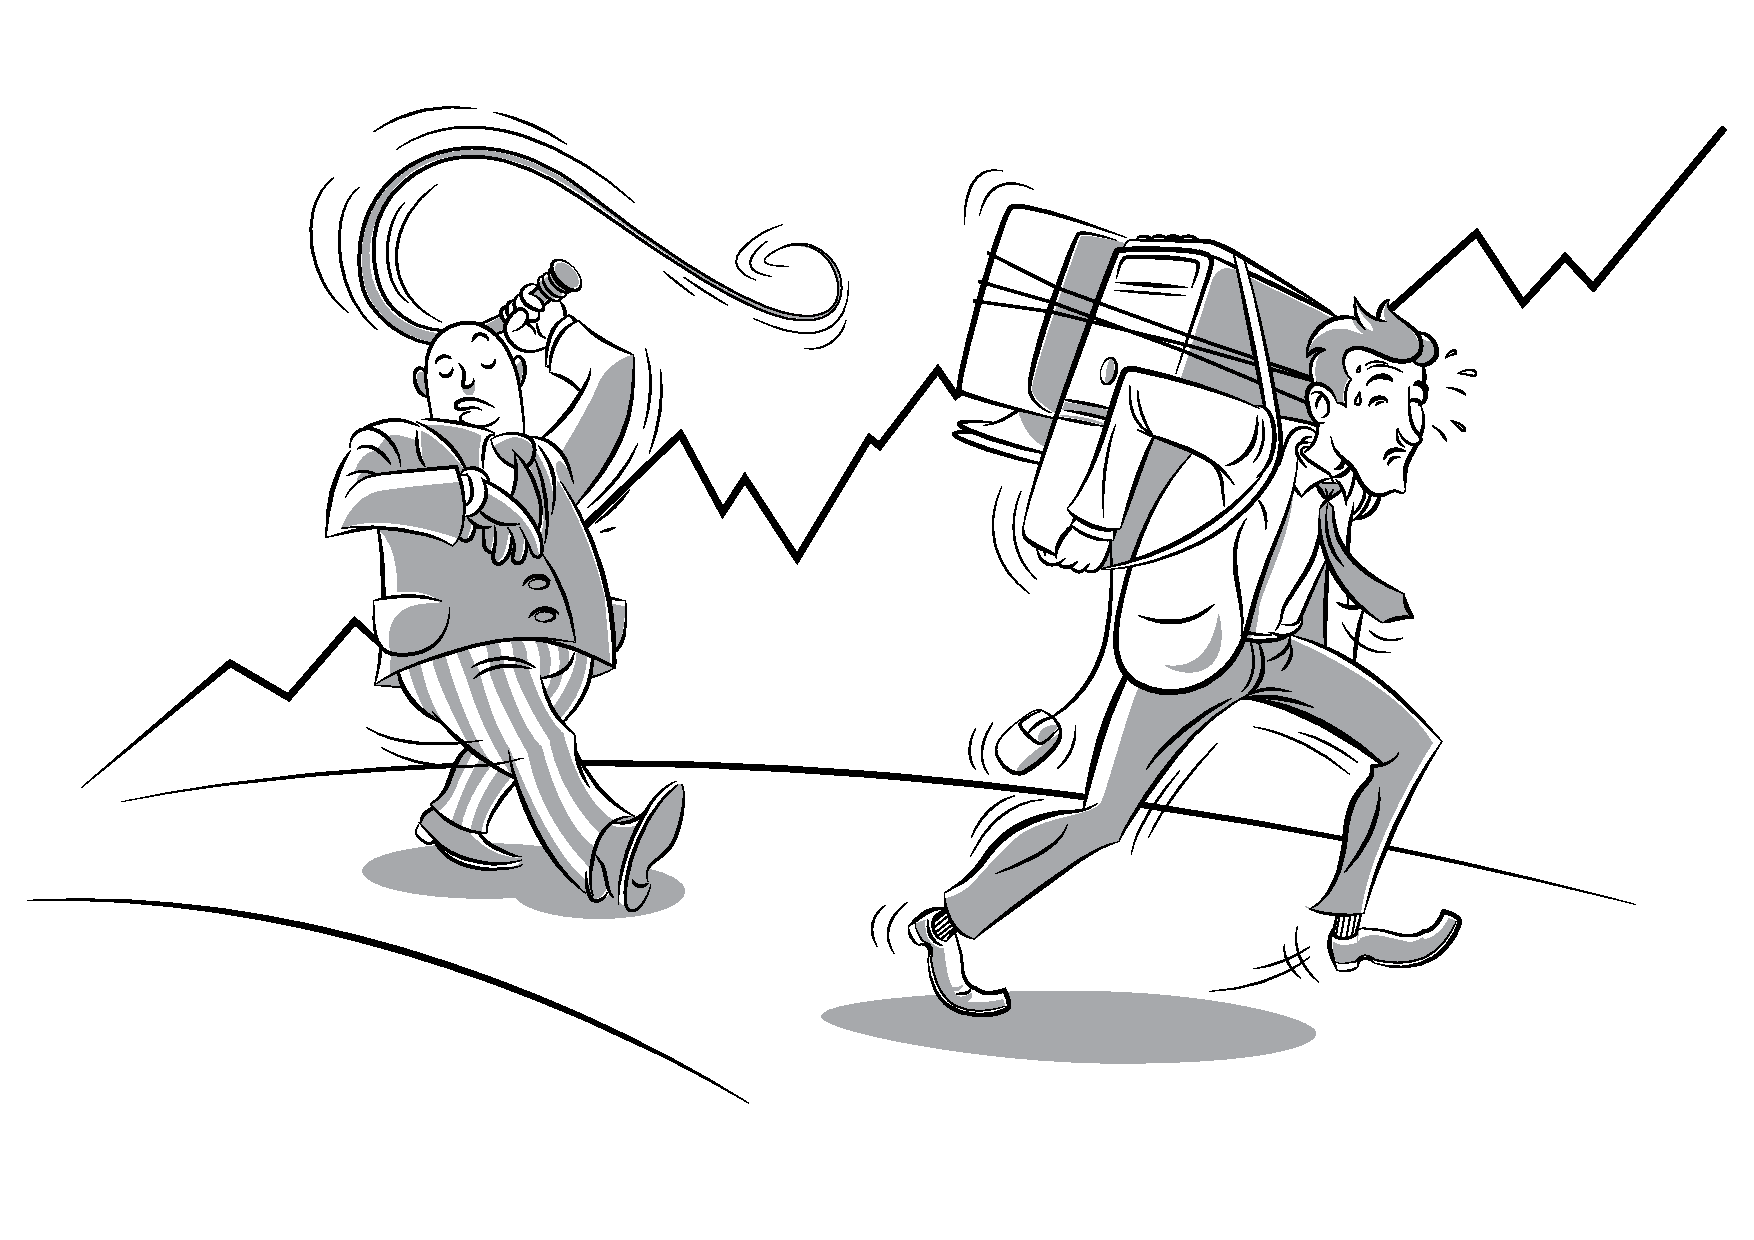
\includegraphics[width=.85\textwidth]{Fig_performance_is_everything.pdf}
% \caption{Pressure to publish is increasing everyday.}
\label{Fig:performance_is_everything}
\end{center}
\end{figure*}

Ferry Dizadji of the European Commission has evaluated journal subscriptions and citation statistics and has suggested a similar \textbf{Relative Cost Index}\index{RCI|see{Relative Cost Index}}\index{Relative Cost Index}:

\begin{equation}\label{E:info.production}
    {\rm RCI} = \frac{{\rm CPI}}{{\rm CPI}_{OA}}
\end{equation}

\noindent where $\rm CPI$ is the Composite Price Index, i.e.\@ the geometric mean of the Price per article and Price per citation, and ${\rm CPI}_{OA}$ is the CPI of a non-profit journal in the same category. Again, the lower the RCI the more efficient the journal. \par

Academic institutions should track their research and look at concrete relevant data such as publication efficiency (the cost of publishing divided by scientific impact) and/or the relative cost index, and then use such parameters to encourage researchers to produce influential work at the lowest possible cost. It is very likely that expensive publishers will also score well on ${\rm PE}$ because good citation statistics often result from high-quality production, but the point we are trying to make is that such information should be made transparent. \par

A major misconception in science is that the quality of articles is mainly due to the journal's IF, i.e.\@ its name. What we want to emphasize in this chapter is that the quality of research articles is primarily a result of good ideas and good research (see further Fig.\@~\ref{Fig:what_makes_good_paper}). Production and post-production are important, but the quality comes from the authors. Measures such as JIF suggest that the scientific quality comes from journals i.e.\@ publishers, and that they alone should be used to evaluate the quality of published research. Fig.\@~\ref{Fig:JIF_vs_RAI} clearly shows that JIF has not much to do with the individual impact of articles and so should not be used to evaluate researchers. \par

Note that we do not want to imply here that scientific publishers should be replaced with \emph{quick-and-dirty} systems. On the  contrary, there would not be any science without companies such as Elsevier, Springer, Taylor \& Francis and Wiley. However, our general impression is that access to science could be extended and that the time it takes to get from research to application could be considerably shortened, to the benefit of all.  \par



%%%%%%%%%%%%%%%%%%%%%%%%%%%%%%%%%%%%%%%%%%%%


\begin{partbacktext}
\part{Guide for authors}
\end{partbacktext}

\chapter{Producing scientific information}

So far, we've discussed some of the problems with the current system of science. In this part of the book we provide practical tips 'n tricks on how to produce high-quality papers. The first thing you need to realize is that it's all about having a good idea and a lot of discipline.\par

Papers are born from ideas, i.e.\@ when an author intuitively senses an important discovery. In principle, every idea/discovery can potentially lead to publication (as illustrated in Fig.\@~\ref{F:pubs}). But not all drafts are publishable. So you should first ask yourselves whether your work is truly novel and whether it has a large enough potential audience. In many cases, you may need to face the fact that your ideas are simply not good enough for a top journal (or perhaps not even good enough for any journal). Such work can still be disseminated, but in a different format. Once you are sure, however, that you want to produce a research article, you need to be systematic. Producing scientific publications generally takes place in five main stages:

\begin{itemize}
  \item \emph{Design and preparation of the scientific publication} (experimental design and agreement among co-authors)
  \item \emph{Actual research work} (data collection, data analysis, scientific writing)
  \item \emph{Product filtering} i.e.\@ peer-review, line editing and production of graphics
  \item \emph{Publication and dissemination}
  \item \emph{Post-production} (mainly product marketing).
\end{itemize}

In the following sections we describe these stages. We first focus on preparation and data collection. In chapter~\ref{sec:structures} (page~\pageref{sec:structures}) we focus on the techniques and skills needed to write papers, and in chapter~\ref{sec:submitting} (page~\pageref{sec:submitting}) we provide some pre-submission checklists. We highlight both threats and opportunities and illustrate these with some examples. \par


\section{Design and preparation}\label{sec:preparation}

\begin{quote}
    \emph{``I believe in intuition and inspiration. Imagination is more important than knowledge. For knowledge is limited, whereas imagination embraces the entire world, stimulating progress, giving birth to evolution. It is, strictly speaking, a real factor in scientific research.''}\footnote{Albert Einstein in \emph{``Cosmic Religion: With Other Opinions and Aphorisms''} (1931), p.~97.}
\end{quote}

People generate ideas in different ways. One natural way to come up with ideas is:

\begin{itemize}
  \item \emph{Gather raw material --- specific \& general --- and combine it kaleidoscopically}.
  \item \emph{Digest this material mentally}.
  \item \emph{Drop the problem and do something completely different}.
  \item \emph{Experience the Eureka moment, when the creative idea appears as if out of nowhere}.
  \item \emph{Expose the idea to criticism i.e.\@ test it against the real world}.
\end{itemize}

The creation of ideas is usually a non-linear process. It often happens as the result of complex mental processes that are still not fully understood. Nevertheless, we can create an environment that's conducive to generating ideas. Life on earth developed in physical and chemical conditions over 2 billion years ago. Simple molecules just needed enough energy, water, chemicals and radiation; the rest they figured out themselves. In the same way if we expose a human brain to inspiring ideas and provide materials/tools that it can play with, it is very likely that these will lead to new ideas and hence to new creations. For practical tips on how to improve your creativity by improving your working conditions, see section~\ref{sec:stress} (page~\pageref{sec:stress}) on coping with stress. \par

For Prof.\@ McBratney\index{McBratney}, University of Sydney, the typical cycle of producing a scientific information package is:

\begin{enumerate}
  \item \emph{Generate an important idea}
  \item \emph{Develop it (design the experiment)}
  \item \emph{Think how to test it (choose the right statistical method)}
  \item \emph{Collect data (measure)}
  \item \emph{Test it}
  \item \emph{Publish it}
  \item \emph{Move on to the next idea}$\ldots$
\end{enumerate}

\begin{flushleft}
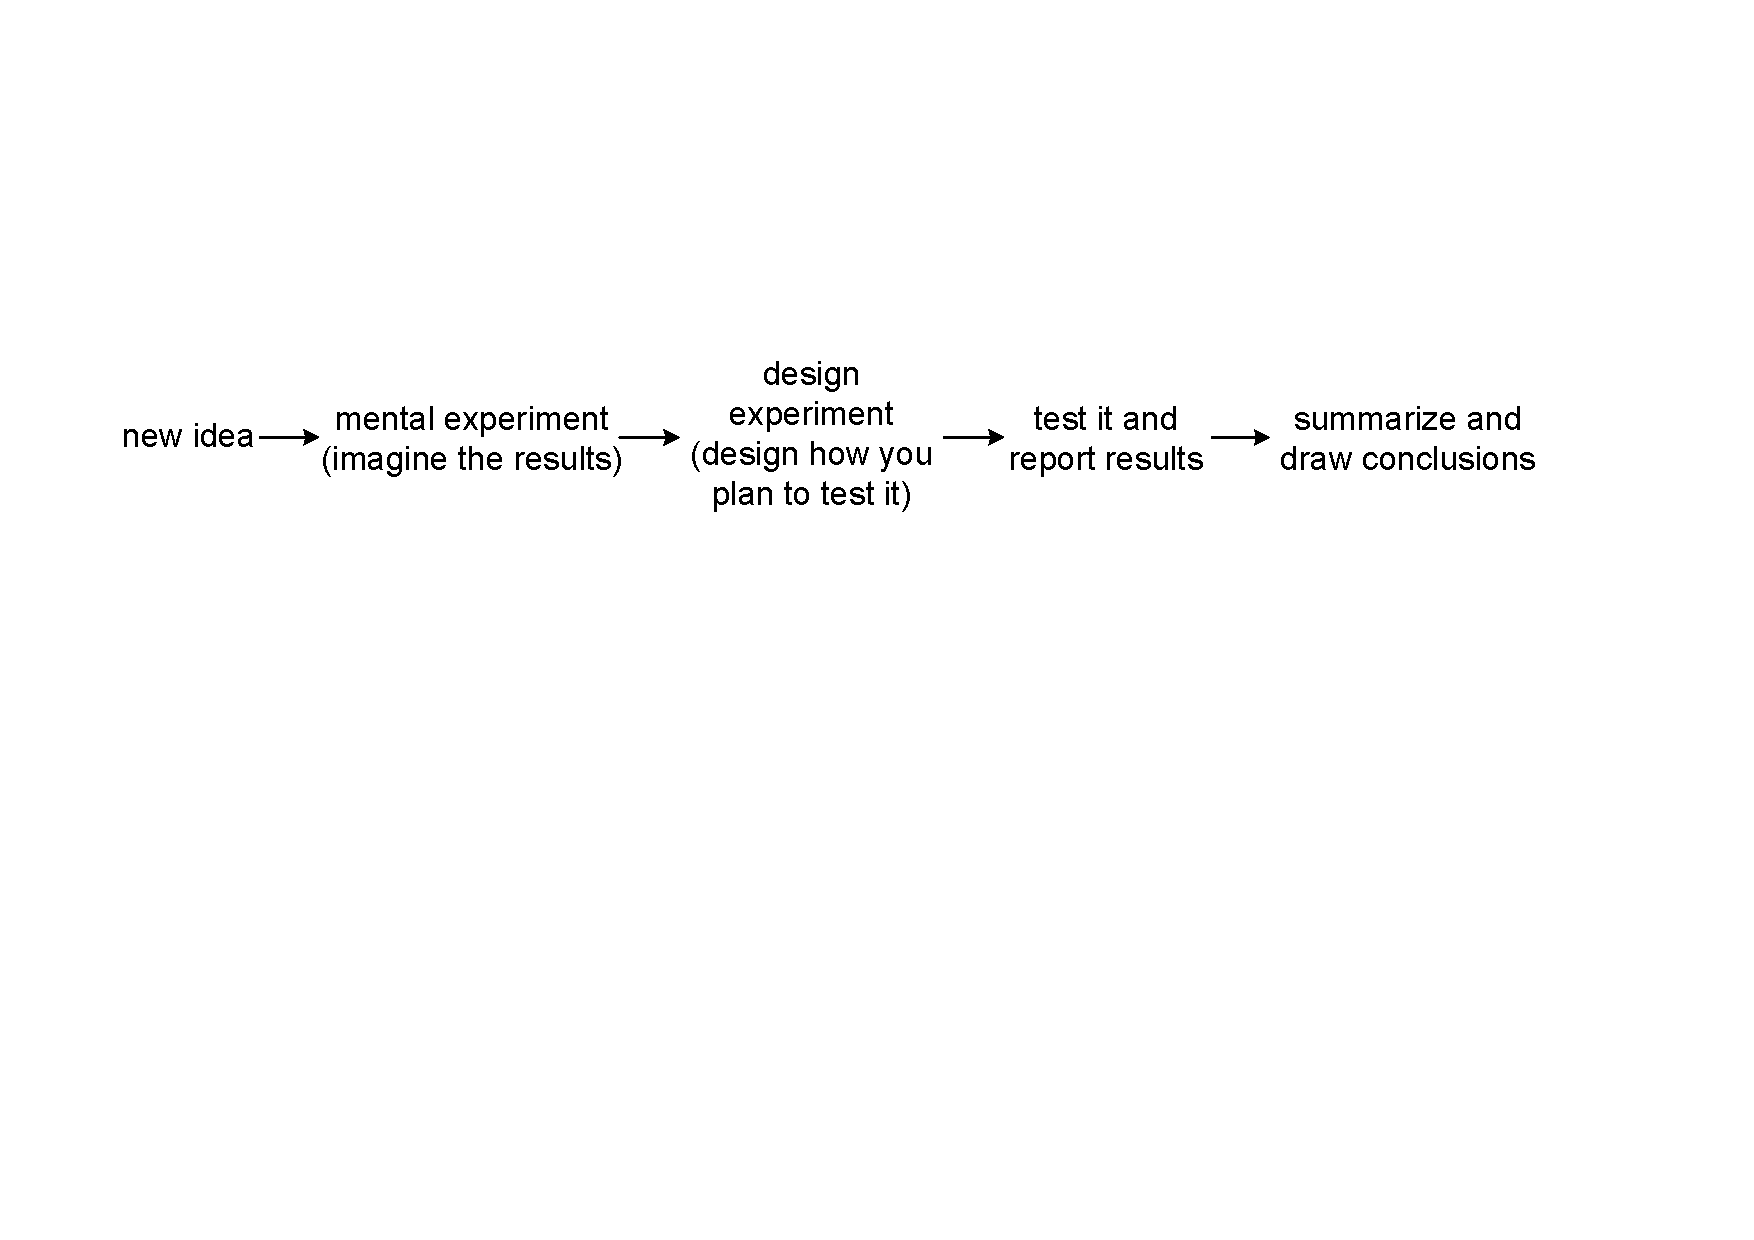
\includegraphics[width=\textwidth]{Fig_new_idea_flow.pdf}
\end{flushleft}

Also for \citet{Creedy2008research}, the pre-writing stage is crucial to improving efficiency. He offers a number of practical tips:

\begin{itemize}
  \item \emph{Attach a time schedule to your writing plan} (aim to finish with several weeks to spare before the deadline).
  \item \emph{Start writing immediately} (write as you go along).
  \item \emph{Establish good working habits and use your time efficiently: work on a bibliography or on tidying up graphics and supplementary materials when you can't work on the main parts of your paper}.
  \item \emph{Arrange regular meetings, be flexible and revise your plan when necessary}.
\end{itemize}

This last tip needs to be emphasized. Science requires flexible agendas; you can't make progress with strict routines. A \emph{live} agenda that can be iteratively adjusted based on initial results and difficulties typically leads to faster progress, because science can be extremely unpredictable \citep{Crump2002}. Problem solving should dictate the way we design science.\par

It's also important to emphasize that many researchers (especially beginners) put themselves under unnecessary stress by seriously under-estimating the time/effort needed to complete project phases. \citet[p.22]{Creedy2008research} thinks that we should be much more pessimistic: \emph{``when planning research projects, produce a generous estimate, fully allowing for the fact that everything takes longer --- then double the time and add some more for good measure.''} \par

Wikihow (a manual that anyone can edit) lists the following key tips on \emph{``How to Conduct Academic Research''}\footnote{\url{http://www.wikihow.com/Conduct-Academic-Research}}, i.e.\@ how to write an essay or review paper on a research topic:

\begin{enumerate}
\renewcommand{\labelenumi}{(\textit{\alph{enumi}})}
  \item \emph{Design your research}: Determine your research topic/question. Understand the difference between primary (original) and secondary (review) research. Determine your scope and time line. Write a research question, which reflects a real problem that needs to be solved. Ideally it should contain variables or other relationships that can be tested.
  \item \emph{Read the relevant literature}: Learn how to find useful sources. Collect some possible sources and begin reading in detail. Find a method to take notes on what you read. Continue to consider new sources.
  \item \emph{Evaluate}: Evaluate the sources you use. Keep your research question in mind. Your source material must help you establish your thesis. Be selective. Don't be tempted to write an exhaustive \textsc{Wikipedia}-style review of the topic.
  \item \emph{Formulate the thesis}: Write your tentative \textbf{thesis}\footnote{This is a single statement of your position on the research question.}\index{thesis}\index{Wikihow}. Think of how to express your point in a single, complete sentence. Make sure this sentence states your opinion.
  \item \emph{Begin writing}: Begin writing your first draft. First sketch a rough outline, which explains the problem you are tackling, a research question (or series of questions) designed to solve that problem, answers to these questions, the implications of those answers, and possible next steps for research.
  \item \emph{Revise it}: Continue writing your first draft with quotes (or paraphrases) from relevant sources, and then revise it.
  \item \emph{Finalize it}: Prepare the final draft. Strictly follow the format of the target journal, by checking its handbook or a general stylebook (e.g.\@ \citet{turabian2007manual}). This includes: title page, page setup and numeration, citations, bibliography style, visuals, sections and titles, etc.
\end{enumerate}

For \citet{Rossiter2010RCS}\index{Rossiter}, reporting on research follows Caesar's proverb \emph{veni}, \emph{vidi}, \emph{vici}, or in other words: I came and applied some methods to attack the problem (\emph{veni}), I saw the following results (\emph{vidi}) and I can now draw some significant conclusions (\emph{vici}). One victory leads to another battle, of course.\par

For Alex McBratney\footnote{Keynote talk at the Pedometrics 2007 conference.}, the keys to success in scientific work are:\index{McBratney}

\begin{itemize}
  \item \emph{engage in deep reflection}
  \item \emph{talk to people}
  \item \emph{use mind-altering devices}
  \item \emph{no Ipod!}\footnote{Hopefully Apple will not take this remark as anti-marketing. The fact is that many modern entertainment devices tend to capture a lot of our attention, with the risk that we lose focus.}
\end{itemize}

Assuming that you have an idea (and frankly, it's not important how you got it as long as it's your own and it's a good one), this needs to be converted into a clear, concise proposal. \par


 \section{The one-page concept paper}\label{sec:one_page_concept}

The first tip for producing relevant, credible, readable scientific information is to carefully plan the whole thing right from the start. Pitch your idea as if you were trying to convince a journal editor of the value of your research. We call this a one-page concept paper. As we mentioned earlier, editors take just a few minutes to decide whether a paper that's been submitted should go to peer review or be rejected. This paper should include the topic, the authors and their roles and responsibilities, your main ideas and assumptions, a broad picture of the experimental setup and a time-line with phases and deliverables. Once the main thrust of your paper has been established, it's much easier to organize the production of the paper. Think of it as a small project.\par

These are some issues that you should definitively consider when preparing a one-page concept paper:

\begin{itemize}\renewcommand{\labelitemi}{$\checkmark$}
 \item What do you want to \emph{`sell'} with this paper? What is the problem that you're addressing and what is the key research question that will lead you to a solution? The research question (and its answer) is the basis of all credible science. Blaise Pascal: \emph{``One cannot really be considered as having a research topic until it can be expressed in the form of a succinct question.''}
 \item Is the topic really\footnote{Often we are sure that the topic we are working on is completely novel. We then find out that it has already been discussed and described, sometimes as long as 50 years ago.} novel?
 \item Who is it intended for: a specialist or broad audience?
 \item What will be its strong aspects?
 \item How are you going to prove your hypothesis and is this proof going to be convincing?
 \item Will you be able to organize the experiment and data processing (resources, support)?
 \item Who will be first, second author, etc., and what will be their responsibilities?
 \item In which form do you want to publish it?
\end{itemize}

\begin{svgraybox}
The most important step in starting a paper is to produce a one-page concept paper. This should include: an important issue (the topic), a clear problem statement, the authors, their roles and responsibilities, your main ideas and assumptions, a broad picture of the experimental setup, and a time-line with deliverables.
\end{svgraybox}

Although it is a good idea to select a target journal early on, at this stage you should first focus on the quality of your research and not think too much about the impact factor of the journal or the number of publications you can produce from your results. Keep in mind that a good paper is one that makes an impact, i.e.\@ one that will be widely read and used by many people to further their research.  \par

As we explained in the first chapter, research publications typically focus on one (or more) of the following:

\begin{enumerate}\renewcommand{\labelenumi}{\textit{\Roman{enumi}}.}
  \item New discoveries (about us and our environment), which could include \citep{Creedy2008research}:
  \begin{itemize}
  \renewcommand{\labelitemi}{$\circ$}
  \item New empirical regularities
  \item A new theory, and/or
  \item Improved understanding of or fresh insights into a problem.
\end{itemize}
  \item New technological developments
  \item Solving open mysteries
  \item Systematization and synthesis of existing knowledge (overview and/or review).
\end{enumerate}

Try to distinguish in which category your paper falls. Perhaps it's all four. In which case it would be rather complex to write such an article. Maybe your work should be split into several articles? \par


 \section{Review your results and repeat the experiment}

\begin{quote}
    \emph{``I only trust those statistics that I've falsified myself.''}\footnote{Winston Churchill}.
\end{quote}

Now you have your master plan, you can proceed with the collection of data, i.e.\@ carry out experiments. The initial results confirm your expectations and you are excited about the whole thing. You would like to publish it as soon as possible. At this stage, it might be wise to review your results and even repeat the experiment several times. Sleep on it. As John Tukey correctly puts it: \emph{``the combination of some data and an aching desire for an answer does not ensure that a reasonable answer can be extracted from a given body of data.''}\par

\begin{figure*}[!htb]
\begin{center}
  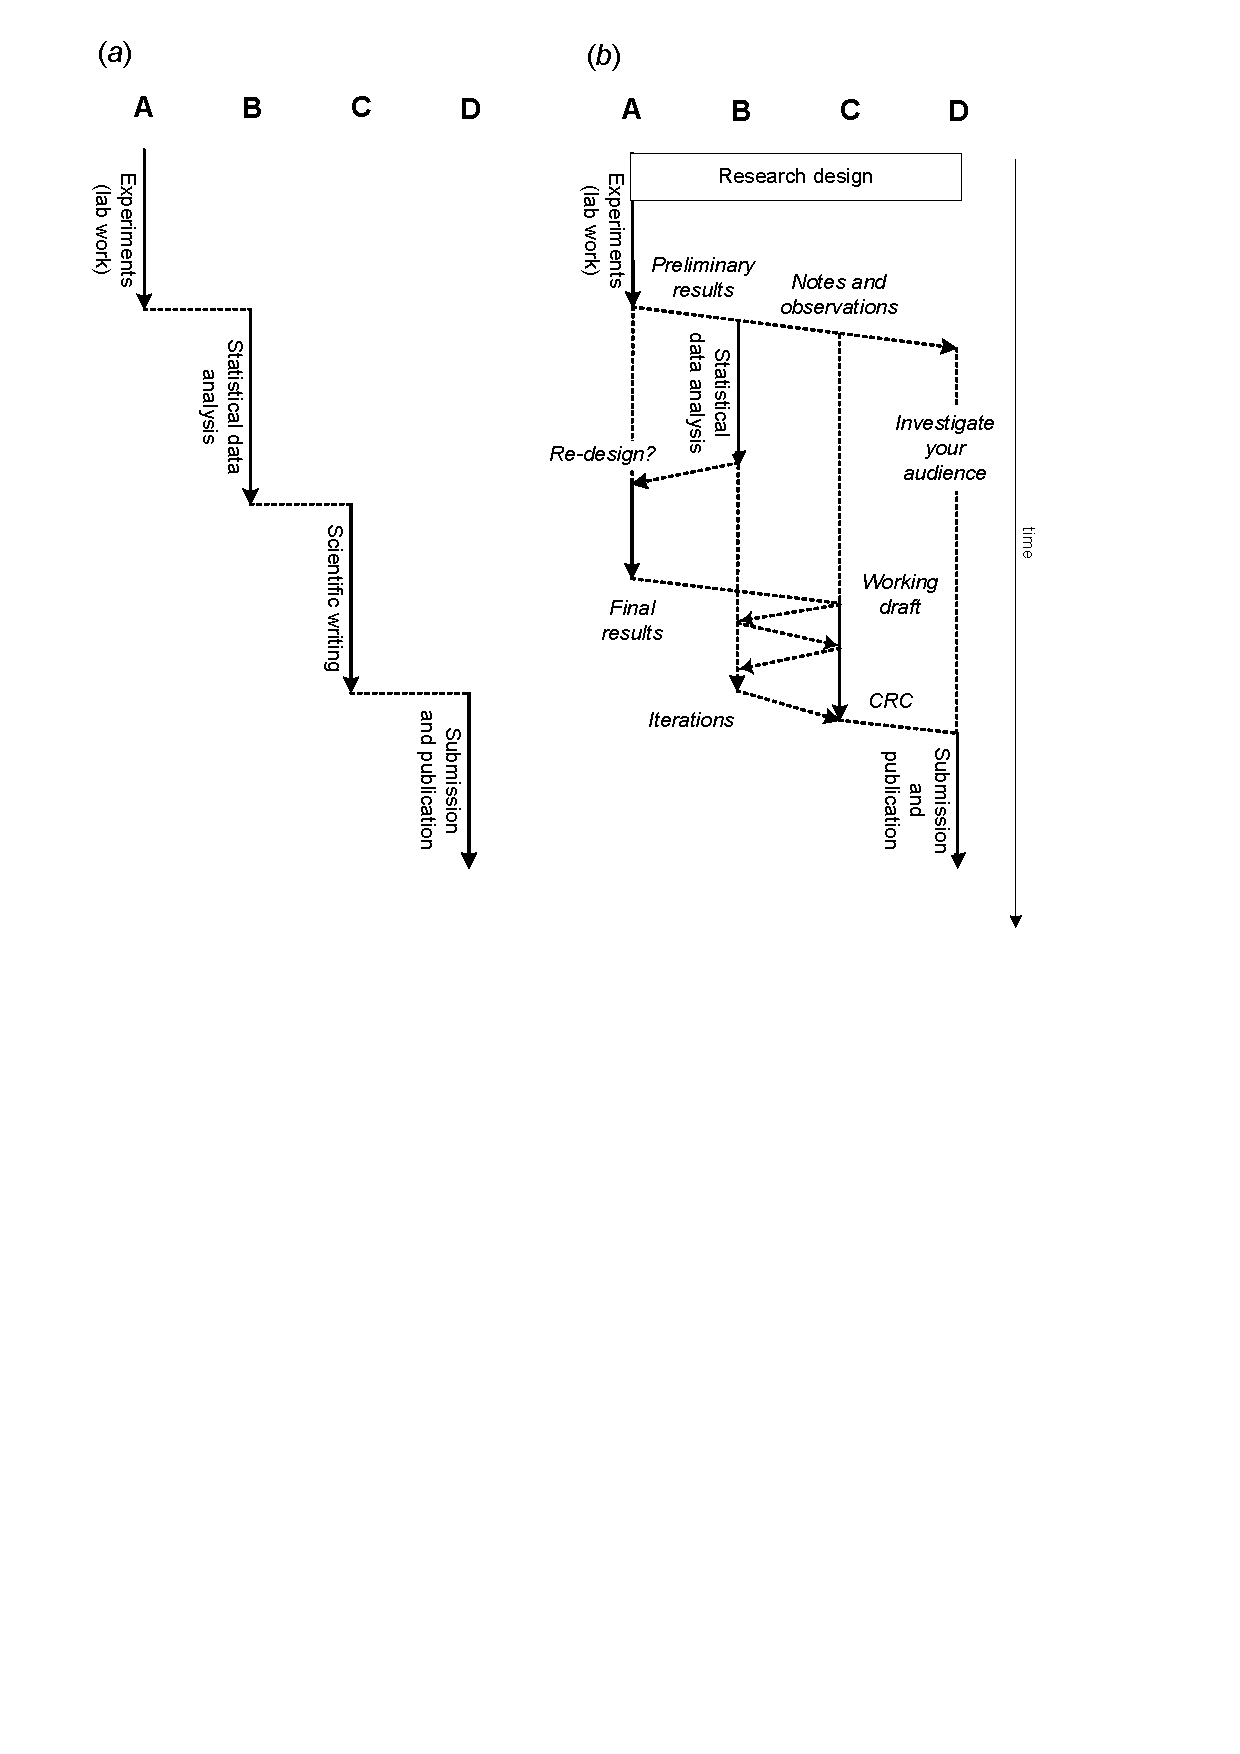
\includegraphics[width=\textwidth]{Fig_paper_production_flow.pdf}
\caption{Scientific paper production phases --- lab work (A), analysis (B), writing (C) and submission (D): (a) the `linear' approach (which almost never works), and (b) the iterative, parallel approach. In practice, evolution of scientific information up to Camera Ready Copy (CRC) is, in fact, highly non-linear with many iterations, resets and re-designs.} \label{Fig:paper_production_flow}
\end{center}
\end{figure*}

The worst-case scenario is that you get your paper published and then find out that some aspects or elements were incorrect or wrongly interpreted. Once people find out, you get a bad reputation and you will have a much lower chance of publishing similar papers in future. So, although you scored a publication, you've damaged your career. Prof.\@ McBratney suggests: \emph{``spend more time thinking how to test a model before it's too late.''}\index{McBratney} \par

\begin{svgraybox}
The most critical parts of your article are likely to be the evidence and interpretation. Spend time thinking how to make your arguments more convincing. Reconsider your results and, if possible, repeat the experiment several times.
\end{svgraybox}

This brings us to another big problem of modern science --- impatience. Authors are often impatient to publish, so they hide unexpected findings or things that they cannot explain. Sometimes, research projects can lead to what is called \emph{`negative'} results --- proving that the proposed methodological or technological improvement does not fit expectations or does not help solve some practical problem. \citet{Creedy2008research} points out that even such disappointing results can be useful and should certainly not be dismissed. In fact, some of the best articles in the history of science focused on something that DID NOT WORK. Are you aware that the most significant discoveries\footnote{For example, electricity, telephone, R\"{o}ntgen rays, cosmic background radiation, etc. See a book on this topic by \citet{Newman2000DM}.} in the world happened unexpectedly, through serendipity or even error? Really important ideas only become clear in retrospect. Great ideas might be emerging right now, but we don't know it. In other words, if you are too sure about the results you expect and if there's too much routine in your work, do not expect to discover something great (see also the rules of science on page~\pageref{F:rules}). For the same reason, always be very flexible and ready to adjust the key topic of your article, depending on what you and your co-authors think is the most significant discovery.\par


 \section{Investigate your audience}

Once you've done several tests and got the same results repeatedly, you can be confident about your discoveries. However, you should not immediately complete the paper. Now is a good moment to investigate your audience, i.e.\@ those who will read and evaluate your work: focus on the audience and readability of the paper. This is nicely emphasized by \citet{Gopen1990}: \emph{``An academic paper cannot exist without the interpretation of each reader. If the reader is to understand the writer, the writer has to know what the reader needs. We can't be sure that even a single sentence we write will mean the same to every reader; all we can do is increase the chances that most readers will interpret our writing the way we intended.''}\par

The best way to find out how potential reviewers will receive your paper is to communicate some preliminary results at a research conference or seminar. Communicating your preliminary results and key ideas to potential reviewers will give you insight into what they see as strong points and what they criticize. You can get such feedback in few hours (if you send a paper to a journal, you will have to wait for months). By giving seminars you can also practice putting your thoughts into words and then into arguments.\par

If you do not get any questions about your work, this is a bad sign. Either your colleagues are not interested in the topic, or they have difficulties understanding it, or you have not emphasized the key points in your presentation. Also, if you offer too many ideas/results (even good ones), this can tire an audience and they will not be receptive to your work. The same will probably happen with the paper. Sometimes, throwing things out of the paper really helps --- \emph{less is more}! Many investigations\footnote{See for example the work of \citet{Hartemink2002S} about publishing in soil science.} have shown that shorter, more focused papers generally have a higher impact. One of the reasons why short is better is because the authors have had to put more work into compressing their work. As Blaise Pascal once said: \emph{``Je n'ai fait celle-ci plus longue que parce que je n'ai pas eu le loisir de la faire plus courte''} or \emph{``I have made this (letter) longer than usual, only because I have not had the time to make it shorter.''} \par

Research conferences are also a good place to find out more about the topics that your colleagues are working on. It's not only important to find out what others think about your ideas, it's also important to know what other people are working on at the moment. The best scenario is that your topic (research problem) is discussed heatedly by many other scientists, i.e.\@ it's \emph{`hot'}. This is definitively a sign that you should start preparing the first draft of your paper. \par


\section{Ten simple rules}\index{ten simple rules}

\begin{quote}
\emph{``First principles, Clarice. Simplicity. Read Marcus Aurelius. Of each particular thing, ask: what is it, in itself, what is its nature...? ''} \footnote{The first simplicity principle of Hannibal Lecter that helped agent Clarice Starling solve the case of a serial killer. From \emph{``The Silence of the Lambs''} book by Thomas Harris.}
\end{quote}

PLoS has published a collection of \emph{Ten simple rules}\footnote{\url{http://collections.plos.org/ploscompbiol/tensimplerules.php}} for various aspects of scientific work. The ten rules for doing best research according to Hamming are \citep{Erren2007PLoS}:

\begin{enumerate}
  \item \emph{Forget modesty and say to yourself ``I want to do something significant.''} (Go Big or Go Home)
  \item \emph{Prepare your mind --- luck is a marriage between opportunity and preparation.}
  \item \emph{Start publishing young.}
  \item \emph{Brains are not enough; you also need courage.}
  \item \emph{Make the most of your working conditions --- don't blame the tools.}
  \item \emph{Work hard and effectively.}
  \item \emph{Believe and question your hypothesis at the same time.}
  \item \emph{Focus on what is important for society.}
  \item \emph{Be committed to your problem.}
  \item \emph{Leave your (office) door open --- don't get too isolated.}
\end{enumerate}

Likewise, \citet{Bourne2005} compiled ten simple rules for getting published:\label{sec:bourne_rules}\index{ten rules, for getting published}

\begin{enumerate}
  \item \emph{Read many papers, and learn from both the good and the bad work of others.}
  \item \emph{Learn to be objective (as the journal editors) early. The more objective you can be about your work, the better that work will ultimately become.}
  \item \emph{Look at the masthead of the journal in which you plan to publish. Good editors and reviewers will be objective about your work.}
  \item \emph{Learn to write well in the English language.}
  \item \emph{Learn to live with rejection.}
  \item \emph{Do not ignore the essential ingredients of good science/reporting: novelty, comprehensive coverage of the literature, good data, good analysis and thought-provoking discussion, good organization of the document, appropriate use of tables and figures, right length, writing to intended audience.}
  \item \emph{Start writing the paper the day you have the idea of what questions to pursue.}
  \item \emph{Become a reviewer early in your career.}
  \item \emph{Decide early on where to try to publish your paper.}
  \item \emph{Quality is EVERYTHING. Better publish one paper in a quality journal than multiple papers in lesser journals.}
\end{enumerate}

Such rules of thumb won't necessarily work for every field of research or for every individual, but they are based on decades of experience from a variety of research fields and cultures, so are certainly worth considering. Although it might seem simplistic to reduce everything to simple rules, these are essentially sound. \par

\begin{figure}[!hbt]
 \begin{center}
  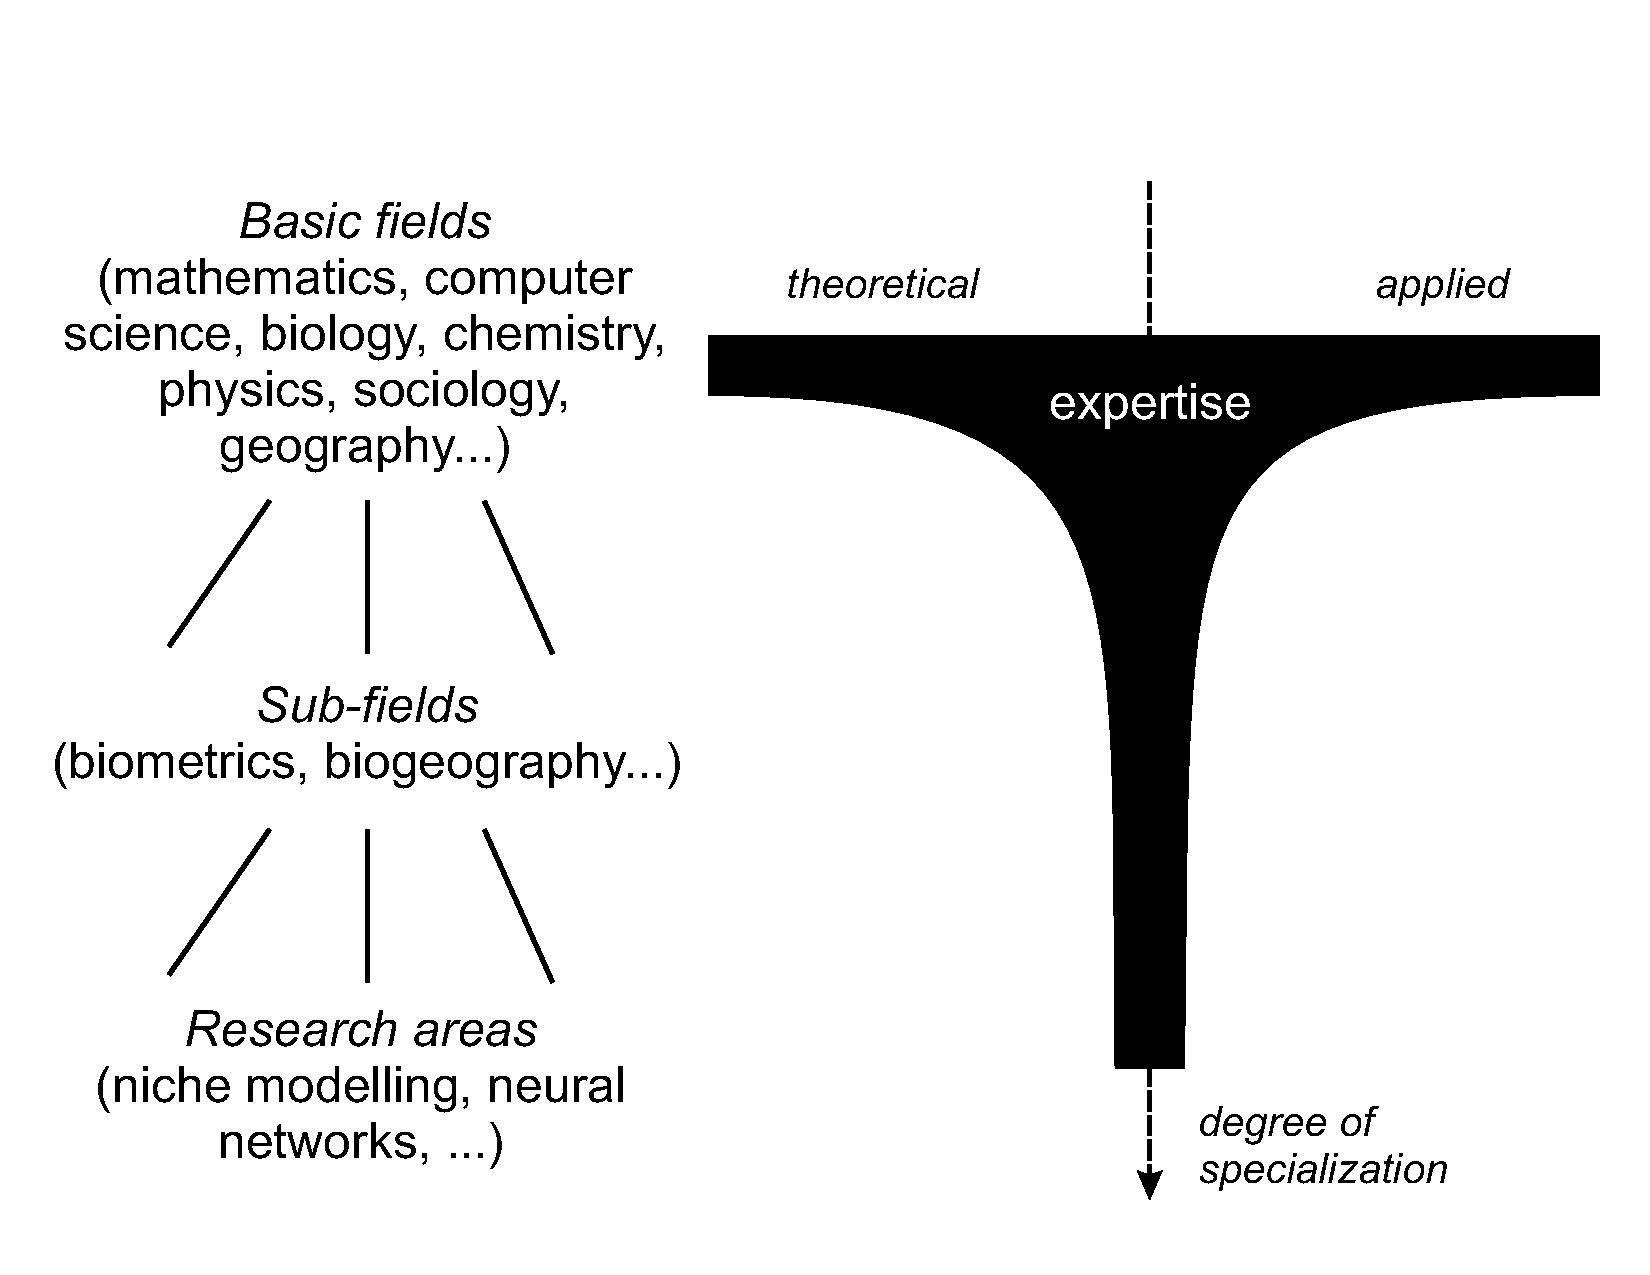
\includegraphics[width=.75\textwidth]{Fig_T_shaped_skills.pdf}
 \caption{The concept of T-shaped skills: a modern researcher is expected to be a hybrid between a generalist and a specialist, with equal ability in the applied and theoretical sides of knowledge.} \label{Fig:T_shaped_skills}
 \end{center}
\end{figure}

So, the first question you need to answer is: how ambitious are you? Obviously, if you want to do top-class work, you will need to work hard: six of the ten rules refer to preparation, commitment, and focus. On the other hand, there's no need to be obsessed about your work. In fact, the best ideas come from a healthy body and soul and not from obsession and isolation. Participation in regular sporting activities or other non-intellectual pursuits provides a valuable diversion from work \citep{Creedy2008research}. For examples, sports such as jogging, swimming or cycling are excellent activities to get fit while allowing your unconscious mind to continue processing intellectual problems (see section~\ref{sec:preparation} on generating ideas).\par

Group sports are also useful for developing social skills and strengthening your stamina and crisis management skills. Another useful way to relax intellectually and get inspiration is to read popular science books and science articles in the media (as long as these articles are based on systematic research and not speculations). Seminars can also be very inspiring, even when the topics discussed are very different from your own work.\par

Many sociologists and managers think that intellectual workers with T-shaped competencies are better at coping with real-life problems (see Fig.\@~\ref{Fig:T_shaped_skills}). Thus, investing in your general knowledge could be beneficial for your success as a researcher. \par

Rik Leemans, editor in chief of the journal Current Opinion in Environmental Sustainability and author of several influential papers, when asked about the secrets of success for writing winning articles, refers to the following \emph{spices}:

\begin{itemize}\renewcommand{\labelitemi}{$\checkmark$}
  \item \emph{the team}
  \item \emph{the guts to be innovative}
  \item \emph{effort spent on producing a new tool and/or new large database}
  \item \emph{effort spent on promoting it (through workshops and press releases)}.
\end{itemize}

Note that teams increasingly trump \emph{solo} authors: teams typically produce more frequently cited research than individuals do, and this advantage has been increasing over time\footnote{In the old days solo authors were more likely to produce exceptionally high-impact research.} \citep{Wuchty2007}.\par

Furthermore, for Leemans, the key to success is to produce papers that are winners in at least four categories:

\begin{itemize}
  \item \emph{it's a story}
  \item \emph{it's interesting}
  \item \emph{it's clear (easy to grasp)}
  \item \emph{it will sell}.
\end{itemize}

Leemans suggest that, in order to improve readability, authors should always use the language of their target audience and define or \emph{`translate'} unusual terms.\par

\begin{svgraybox}
The key to producing highly influential articles is: (1) focus on a topic that is relevant, (2) get the best co-authors on your team, (3) demonstrate your points by using clear examples, (4) package your paper with accompanying materials (posters, software, web-sites, video-demos, promotional materials).
\end{svgraybox}\label{R:success}

The European Association of Science Editors\index{EASE guidelines} (EASE) has produced a list of guidelines for writing research articles and other scientific publications\footnote{\url{http://www.ease.org.uk/guidelines/}}, as a result of long discussions on the EASE Forum and during the EASE 2009 conference in Pisa. Here is a summary:\label{sec:EASEguidelines}

\begin{enumerate}
  \item \emph{Do not begin drafting the whole paper until you are sure that your findings are reasonably firm and complete}, so that you can draw sensible and reliable conclusions.
  \item \emph{Choose the right journal for your manuscript before you start writing}.
  \item \emph{Do not submit articles that are not 100\% complete}.
  \item \emph{Follow the logical macro-structure suggested by the publisher} --- information is interpreted more easily if it is placed where readers expect to find it.
  \item \emph{Do not include information that is not relevant to your research question(s)}.
  \item \emph{Do not copy and paste} (substantial parts) \emph{from previous publications}.
  \item \emph{Do not repeat information in the article} (with the exception of the abstract, figure legends and concluding paragraphs).
  \item \emph{Reduce the length wherever possible} (delete obvious statements and other redundant fragments).
  \item \emph{Replace long scientific terms and expressions with abbreviations}.
  \item \emph{Express your doubts if necessary but avoid excessive hedging}.
  \item (Unless required otherwise by the editors), \emph{use numerals for all numeric data}, i.e.\@ also for single-digit whole numbers, \emph{except for zero and one} (if without units), and in other cases where misunderstanding is possible. In numbers exceeding 4 digits to the right or left of the decimal point, use thin spaces (not commas) between groups of 3 digits.
  \item \emph{Clearly distinguish your original data and ideas from those of other people and from your earlier publications}.
  \item \emph{Check that you are using correct scientific terms}. Define every uncommon or ambiguous scientific term at first use. Avoid colloquial and idiomatic expressions. If in doubt, replace unfamiliar terms with easily understood terms with a similar meaning.
  \item Add the original names of places to lesser known geographic names.
  \item \emph{Write compact, cohesive and logically organized text}. Each paragraph should preferably start with a topic sentence, with the next sentences fully developing the topic.
  \item \emph{Do not overuse passive constructions}. But keep in mind that the subject of the sentence determines whether active or passive voice is required. The most important thing is to make sure that the sentence subject is the same as the sentence topic.
  \item \emph{Use the past tense when describing how you performed your study and what you found or what other researchers did; use the present tense for general statements and interpretations}.
  \item \emph{Make figures and tables easy to understand without a need for reference to the main body of the article}. Omit data that are not informative. In captions or footnotes of figures, define all abbreviations and symbols that are not obvious. Use text tables when presenting a small set of data.
  \item \emph{Define abbreviations when they first appear in the main body of the text}. Avoid abbreviations in the abstract.
  \item \emph{Do not write about yourself as ``the author(s)''}, as this is ambiguous. Instead, write ``we'' or ``I''. More and more journals prefer this style.
  \item \emph{Ask a thoughtful colleague to read the whole text, in order to see if anything is ambiguous or unclear}.
\end{enumerate}

These suggestions are based on a range of editorial recommendations for authors and translators of scientific articles. \emph{``If authors and translators follow these guidelines before submission, their manuscripts will be more likely to be accepted for publication.''} (EASE) \par



\section{Coping with stress}\label{sec:stress}

\begin{quote}
    \emph{``Life is like riding a bicycle. To keep your balance you must keep moving.''}\footnote{Albert Einstein as quoted in Walter Isaacson, \emph{``Einstein: His Life and Universe''} (2007), p.~367.}
\end{quote}

At the end of this chapter we feel the need to discuss an issue that is highly relevant to successful production of science: managing stress. Stress is a state of critical mental (emotional) and physical disorder or imbalance that can lead to more serious medical and psychological complications (headaches, anxiety, sleep disturbances, RSI\footnote{Repetitive Strain Injury --- damage to the musculoskeletal and/or nervous system that may be caused by repetitive tasks.}). Stress may be due to a number of causes. In the case of research work, these are \citep{Bloomfield2008}:

\begin{itemize}
  \item too many parallel tasks
  \item too much routine work
  \item tension in your professional network (unclear roles and responsibilities)
  \item deadlines
  \item pressure to compete for funding
  \item pressure to publish.
\end{itemize}

Each of these causes can be dealt with by adopting a systematic strategy. For example, too many parallel tasks probably means that you have to learn how to drop out of some collaboration, or limit your tasks to an agreed list. To avoid tension in a group it's often a good idea to increase the frequency of meetings and discussion panels. Spend more time communicating and giving each other a chance to meet and debate. Do not avoid confrontation. As with any project, it's better to have a team that communicates honestly than to pretend that problems do not exist. Likewise, do not hide problems that you cannot explain --- seek help. Deadlines cannot be avoided, but at least you can prepare yourself psychologically (e.g.\@ if you are a graduate student take a look at Fig.\@~\ref{Fig:stress_curve_PhD} to know what to expect). Think of a deadline as like an important game: the further you get in the playoffs, the more serious you need to be. Now imagine a positive outcome (victory). This thought can carry you through the tough times.  \par

You can deal with stress and tension in your professional network by improving your social practice in general. For example, here are some general suggestions on how to improve chemistry with your colleagues:

\begin{itemize}
  \item try meeting your colleagues in an informal setting (e.g.\@ in so-called \emph{``team building''} sessions)
  \item try participating in group sports
  \item visit other research groups and learn from their experiences
  \item visit research groups abroad (e.g.\@ on sabbatical) --- observe how things are organized and what is better (or worse) compared to your own organization
  \item attend summer schools or workshops in a less formal setting
  \item attend conferences that focus on new developments, new techniques and fresh ideas
  \item attend workshops that stimulate brainstorming and interdisciplinary exercises --- \emph{``games are the most elevated form of investigation.''}\footnote{Quote by Albert Einstein.}
\end{itemize}

\begin{figure}[!hbt]
 \begin{center}
  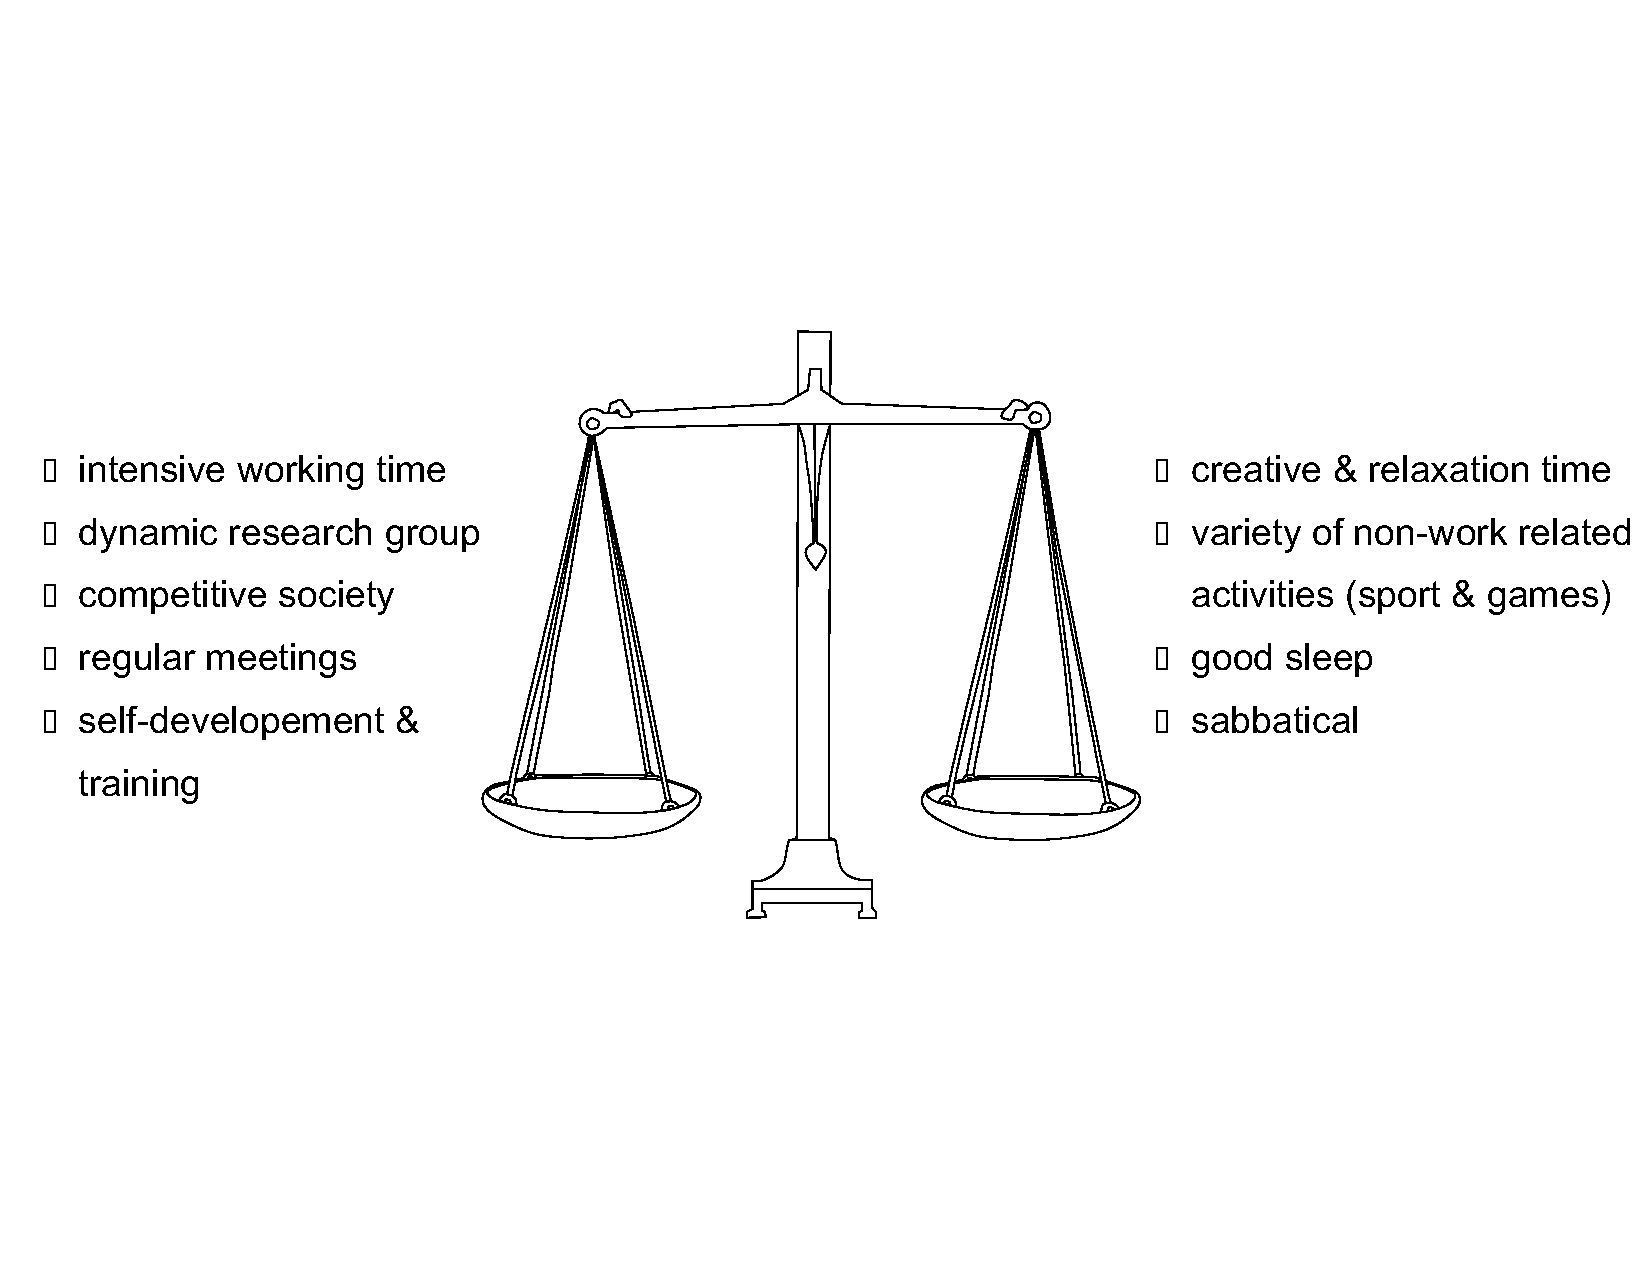
\includegraphics[width=\textwidth]{Fig_libra_antistress.pdf}
 \caption{The key to success in academic work is a balanced combination of hard work and creative relaxation time.} \label{Fig:libra_antistress}
 \end{center}
\end{figure}

Socializing in science is good. Creative individuals inspire each other and great ideas come out of interactive brainstorming --- these people are often your best co-authors. The problem is to find them.\par

Many inexperienced researchers work too hard. The number of hours spent working is, in fact, irrelevant. It's the quality of the scientific work that counts \citep{AscheronKickuth2004}. A working environment can play a key role here. If you're not able to work in an environment that allows you to think clearly and, if you don't have information systems that allow you to run analyses, visualize data, and compare your work with that of others, you're unlikely to be able to develop top science even if you are strongly motivated to succeed. Malcolm Gladwell: \emph{``Success is not a random act. It arises out of a predictable and powerful set of circumstances and opportunities.''}\par

Ultimately, you cannot increase your output simply by extending your working hours. After a point, workaholism and obsession become counterproductive. In fact, you can do damage to yourself and your career if you do not find a good balance between creative, relaxing and working time. \par

\begin{table}[!htb]
\centering \caption{Leo Esaki's rules of thumb for making a career in science. Adapted from \citet{AscheronKickuth2004}.}\label{Tbl:Esaki} % \vspace{10pt}
%\setlength{\extrarowheight}{4pt}
\begin{tabular}{m{.5\textwidth}m{.5\textwidth}}
\toprule
  \emph{Creative side} & \emph{Productive side} \\ \midrule
  \begin{itemize}
    \item focus on relevant topics only
    \item be unconventional and excentric
    \item be stubborn
    \item gain independence \par (of authorities)
    \item do not overload your mind \par with too much information
    \item sleep on ideas
    \item count on luck
    \item create creative chaos!
  \end{itemize}
   &
   \begin{itemize}
     \item generate many publications \par (acquire significant funds)
     \item be systematic and follow conventions
     \item adjust to your research group
     \item listen to advice from your supervisors
     \item memorize important concepts \par (even computer code)
     \item publish as soon as possible
     \item eliminate random effects
     \item tidy up your desk!
   \end{itemize} \\
\bottomrule
\end{tabular}
\end{table}

Leo Esaki, the winner of the Nobel Prize in Physics in 1973, suggested a number of practical rules for making a career in science (see Table~\ref{Tbl:Esaki}). This shows how a researcher has a dual nature --- productive and creative --- and that the two are often in conflict. A combination of creative freedom and systematic work is usually the best strategy. The trick is to know in which situations you can improvise and be relaxed, and in which ones you should be painstakingly precise and focused. \par



%%%%%%%%%%%%%%%%%%%%%%%%%%

 \chapter{Writing research articles}\label{sec:structures}

OK. You have all the data, you're sure about your results and the message that you want to transmit, and you are sure that there is an audience for it --- now you can start writing the paper. If all of the above criteria are satisfied, you might think that writing the article would be the easiest part of the job. But it requires considerable skill.\par

Scientific writing should be easy. Basically, it only requires two tenses: simple present \& simple past, so scientific writers only have to master a narrow selection of the rich range of possibilities within the language. However, inexperienced and experienced scientists alike tend to imitate dense nominalized, depersonalized writing styles and stock phrases, such as \emph{``it has been shown that$\ldots$''} and \emph{``it was observed to$\ldots$''}. We need to return to some simple ground rules for clear, connected readable style.\par

Writers of science want a simple \emph{``recipe''} to help them write readable, scientifically credible journal articles. They want to write their articles as quickly as possible and get on with their research. The approach we present below provides three levels of structure that form the basis not only of the article, but also of logically organizing scientific ideas:

\begin{itemize}
  \item \emph{Macro level}: the overall structure of the article (what goes where)\index{IMRaD}
  \item \emph{Meso level}: the structure of paragraphs --- presenting and supporting scientific messages
  \item \emph{Micro level}: the structure of sentences --- the basic building blocks that tie the whole thing together.
\end{itemize}

Because information is much easier to interpret if it is placed where most readers expect to find it, many scientific articles follow the broad IMRaD macro structure (Introduction, Method, Results, and Discussion). This provides a kind of road map for readers. In particular, writing the methods and results sections can be pretty straightforward.\par

You can use the overall structure of the article discussed in this chapter (see also the appendix) as a template for organizing the ideas and messages that you want to publish. In later sections, we will work on building effective paragraphs (meso level) and sentences (micro level) so that you can clearly present these messages in each section of the article. Then, we will provide some practical advice on how to improve the flow of the paper and increase its readability. Finally, in the appendix you can find a series of steps that will help you organize your article from initial idea to camera-ready-copy.\par


\section{Establishing a framework for research papers: a recipe}\index{research article!recipe}

\begin{quote}
    \emph{``The last thing one knows in constructing a work is what to put in first.''}\footnote{After \citet{Creedy2008research}}
\end{quote}

You could think of writing a research paper as a bit like constructing a house. We start by putting down foundations and building a frame --- its macro-structure. The macro-structure of a manuscript is reflected in the major headings. As mentioned previously, most journals in the world have accepted the \textbf{IMRaD}\index{IMRaD}\index{research article!structure} structure as the international standard. For example, the International Committee of Medical Journal Editors promotes use of uniform rules when preparing manuscripts submitted to Biomedical journals --- \textbf{the Vancouver guidelines}\footnote{\url{http://www.icmje.org/manuscript_1prepare.html}}\index{Vancouver guidelines}. The Vancouver Rules are also accepted as the basis for publication practice by Committee on Publication Ethics (COPE\index{COPE}), Deutsche Forschungsgemeinschaft (DFG), and similar organizations. \par

Ed Hull's\index{Hull} ten-step recipe for making the IMRaD structure work looks like this\footnote{This outline includes material developed by the experienced writing trainer Ed Hull.}:\index{recipe}

\begin{description}
  \item[\textsc{The Introduction}] \hfill \\
      \begin{enumerate}
      \item \emph{Describe a big problem that needs to be solved} --- Journal editors reject articles because the point of the research --- its relevance --- is not immediately and obviously clear. Right at the top of the Introduction show the relevance of your research --- present the big problem that your research helps to solve. A word of warning here, presenting a gap in knowledge is not enough. What we need to know are the consequences of that gap in knowledge.
      \item \emph{State your strategy to help solve the problem} --- This part of the Introduction sharpens the focus on the point of the research. It takes the reader step-by-step from what is already known about the problem to what is unknown about the problem --- it logically leads the reader from the ``big problem to be solved'' to the specific research question.
      \item \emph{State a specific research question/hypothesis whose answer/test will help to solve that problem} --- This needs to be specifically stated in terms of measurable/observable independent and outcome variables and their relationships that your methods were designed to determine. Note that such explicit wording helps the reader to understand your Methods section. A major reason for rejection is that no research question is clearly stated.
    \end{enumerate}
\item[\textsc{Methods}] \hfill \\
      \begin{enumerate}
      \setcounter{enumi}{3}
      \item \emph{Describe the methods used to answer that question} --- This section will differ depending on the type of research, but 3 main items need to be emphasized: (1) \emph{What was studied}, (2) \emph{How the data was collected/observed} and, (3) \emph{How the data was analyzed to determine relationships between the independent and outcome variables}. This section reports what was done --- historical facts --- and must therefore be written in the past tense.
      \end{enumerate}
\item[\textsc{Results}] \hfill \\
      \begin{enumerate}
      \setcounter{enumi}{4}
      \item \emph{Describe your findings} --- This section should link directly to the Methods section and emphasize 3 main messages: (1) \emph{The characteristics of the objects you are investigating}, (2) \emph{Results = data that relates to the research question}, (3) \emph{The relationships (e.g.\@ correlations) between the independent and outcome variables that were determined}. Just as in the Methods section, this section reports historical facts --- what was found --- and must be in the past tense.
      \end{enumerate}
\item[\textsc{Discussion}] \hfill \\
      \begin{enumerate}
      \setcounter{enumi}{5}
      \item \emph{Answer the research question} --- An answer to a research question is a present tense statement of the author's interpretation of his/her results. It links directly back to the research question/hypothesis stated in the Introduction and, therefore, it uses exactly the same words that were used to state the question/hypothesis. As an expert in your field, readers expect you to interpret your results. A word of warning here, do not summarize/repeat your findings in the past tense. Such a repeat is not an interpretation of those findings. Interpretations must be in the present tense. This blunder quite often leads to rejection.
      \item \emph{Support that answer} --- The author must support the answer to the research question. This can be done in several ways: (1) \emph{by showing how the factual findings, expressed in past tense, support it}, (2) \emph{by relating the findings to the work of others}, (3) by \emph{presenting theoretical considerations that support it}.
      \item \emph{State the limitations of that answer} --- Every research study has limitations, even yours (I suggest a subheading ``Limitations'' in the Discussion section). Explicitly state the limitations of your study, and show how they restrict generalization of your answer. Inadequate discussion of limitations is often a reason for rejection.
      \end{enumerate}
\item[\textsc{Conclusions}] \hfill \\
 (I suggest a subheading ``Conclusions'' at the end of the Discussion section.) This subsection should clearly state 2 main messages:
      \begin{enumerate}
      \setcounter{enumi}{8}
      \item \emph{Explain the practical/theoretical consequences of the answer} --- Here, you should point out the value of your work. This relates directly back to the problem stated at the beginning of the Introduction. It clearly shows how the work takes a step toward solving that problem.
      \item \emph{Propose a next step to help solve the original problem} --- One research study seldom solves a big problem. But you --- as an expert in your field --- need to \emph{``stand above''} the details of your work and tell us a possible next step toward solving the problem. A next step could be: (1) \emph{a new research question}, (2) \emph{a refinement of the present study to reduce limitations}, (3) \emph{a protocol that can be used to implement findings}.
      \end{enumerate}
\end{description}

So the key components of a research article are: (1) a significant problem, (2) a strategy for helping to solve it, and (3) possible implications of results for the current state of knowledge. Put these major points on paper and expand your article from this core structure. For more details about the purpose of each section, see the appendix. \par


\section{Basic principles of logical reasoning}

\begin{quote}
    \emph{``No! Scientists do not compromise. Our minds are trained to synthesize facts and come to inarguable conclusions. Not to mention Sheldon is bat-crap crazy.''}\footnote{Leonard responding to Penny's proposal to make peace with Sheldon; from \emph{The Big Bang Theory} TV series created by Chuck Lorre and Bill Prady.}
\end{quote}

The basic skill required to produce new information/knowledge is logical reasoning. Especially in the applied sciences, one relies not only on mind experiments, but also tries to back up claims by using evidence --- proofs, examples and/or arguments. \textbf{Argumentation}\index{logical reasoning} is reasoning designed to arrive at the best approximation of truth using proofs --- \emph{``a constructive debate to reach a solution''} \citep{Rossiter2010RCS}\index{Rossiter}. In the most simple terms, an argument consists of a proposition that is backed up by evidence, connected by some warrant (or justification) with a modal qualifier that expresses the extent of the proposition:

\begin{flushleft}
 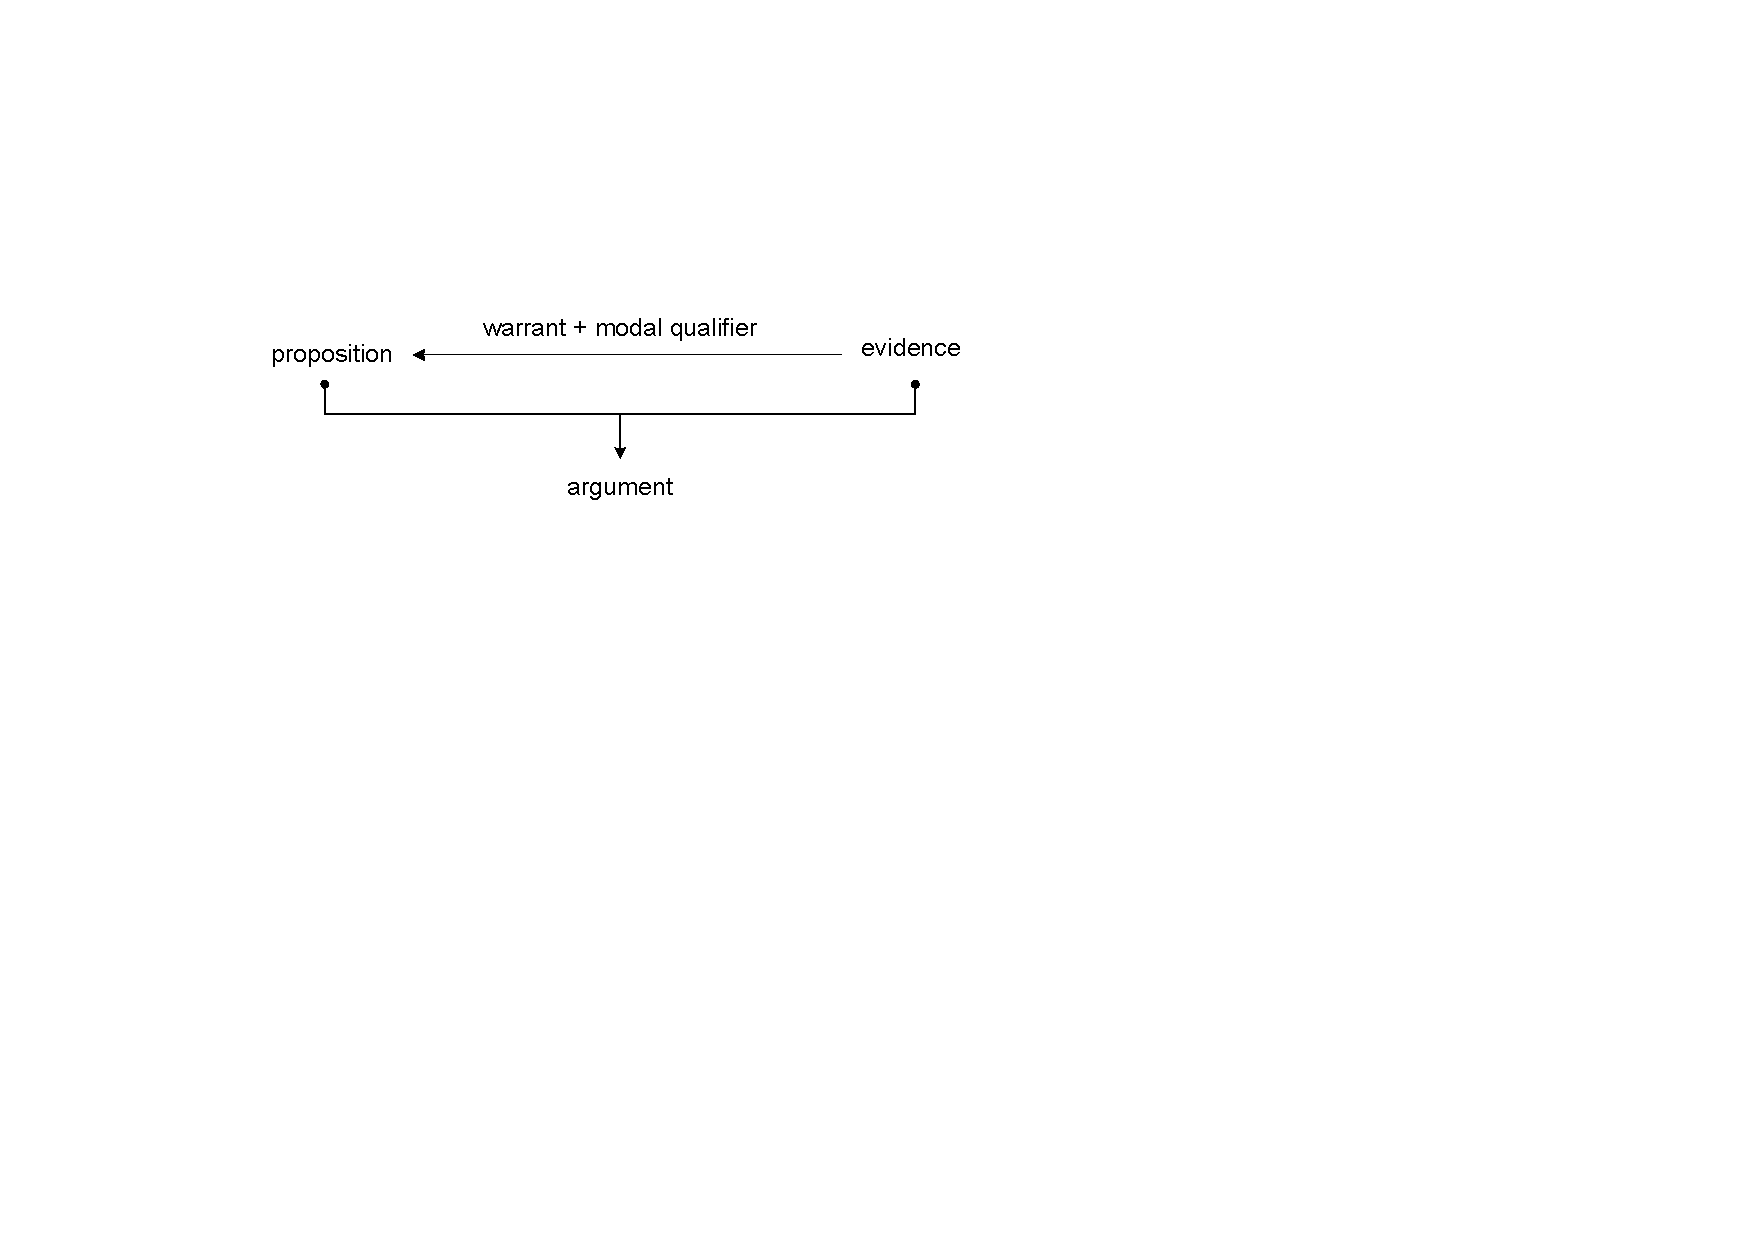
\includegraphics[width=.7\textwidth]{Fig_argumentation.pdf}
\end{flushleft}

Argumentation in a research paper follows a circular path (Fig.\@~\ref{Fig:macrostructure_basic_flowchart}). We start with an assumption\index{research article!assumption} (working claim), then build our case (provide evidence), then make the final claim and justify it with previous arguments. In that sense a research paper is an extensive and detailed version of the argumentation process \citep{turabian2007manual}. \par

\begin{svgraybox}
Clarity of writing follows clarity of thought. So first think what you want to say. Then write it down as simply as possible.
\end{svgraybox}

A research paper can contain several arguments and/or micro-arguments, which are usually interconnected. In principle, every new proposition or claim the authors make in a research paper should be supported by evidence. The evidence could be authors' own data, or other people's data, but a general expectation in any research paper is that we repeatedly present evidence for every new claim we make.\par

\begin{figure}[!hbt]
 \begin{center}
  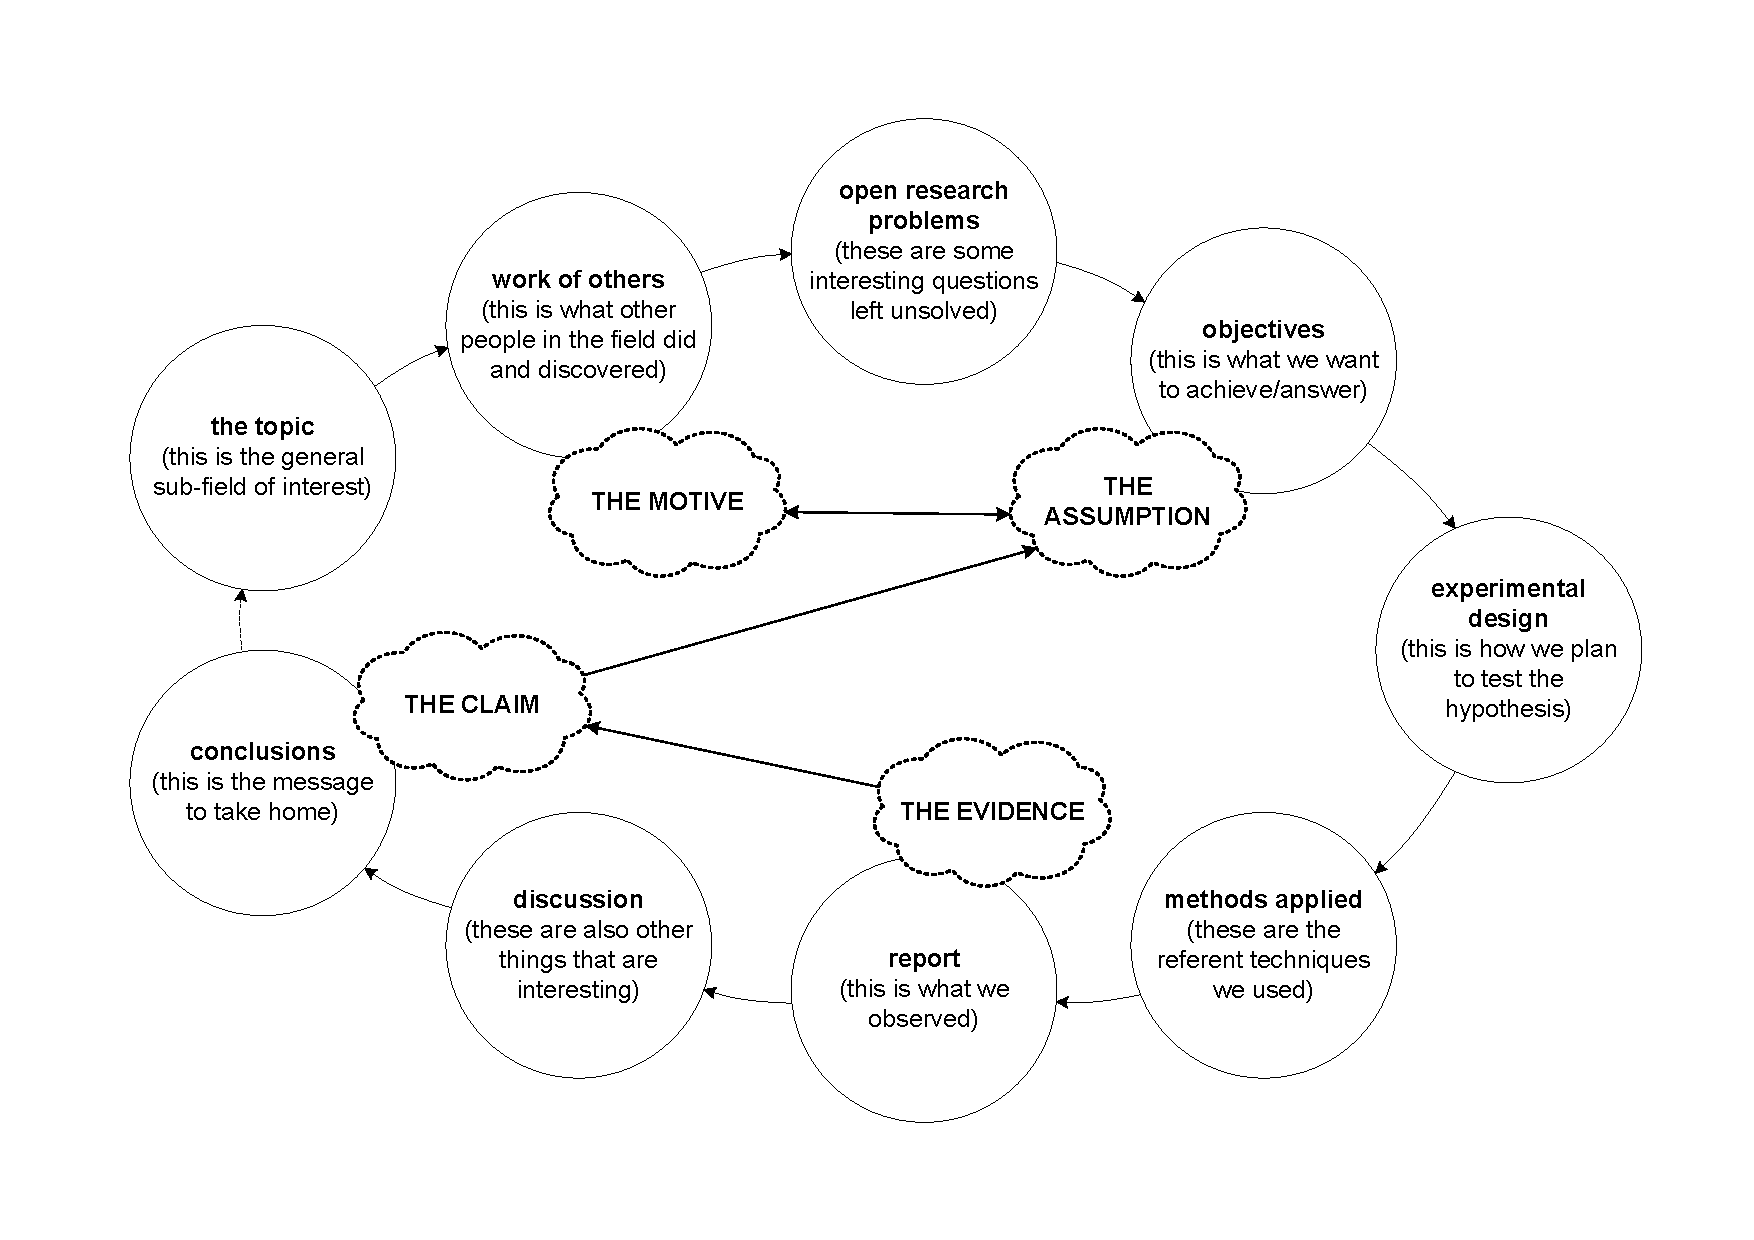
\includegraphics[width=\textwidth]{Fig_macrostructure_basic_flowchart.pdf}
 \caption{Logical steps in a research paper. Research papers are in essence circular because conclusions refer to claims made at the beginning; likewise, each discovery leads to another cycle of research.} \label{Fig:macrostructure_basic_flowchart}
 \end{center}
\end{figure}


In addition, no claim can ever be absolutely universal, so it needs to include a modal qualifier i.e.\@ it should clarify under which conditions the claim is correct. This issue is further discussed in section~\ref{sec:specific} (page~\pageref{sec:specific}). The formal structure of logical reasoning is not as important as the quality of the evidence and order of the reasoning. For some examples of how to build arguments see \citet{Rossiter2010RCS}.\par

For Edward Tufte\footnote{\url{http://www.edwardtufte.com}}, a presentation can be much improved if the presenter emphasizes three key elements: \emph{the message} (going from: problem $\mapsto$ relevance $\mapsto$ solution), \emph{credibility} (why are you the best person to present this work?) and \emph{originality} (e.g.\@ new visualization concepts, new technologies).\index{how to improve presentation}\par

Logical reasoning is crucial. An experienced reviewer can easily scan a research paper and detect poor argumentation --- usually due to a lack of evidence and/or a claim that is too general. The poorer the arguments, the less credible the paper is. Here are some common causes of flawed arguments (based on \citet{AscheronKickuth2004}):\index{flawed arguments}

\begin{itemize}
  \item \emph{ambiguous and vague terms} (your terms are not unequivocal and concrete)
  \item \emph{wrong evidence} (your results do not match your research question)
  \item \emph{incomplete evidence} (what is the uncertainty of your evidence?)
  \item \emph{wrong logical reasoning} (your conclusions do not make sense)
  \item \emph{unconvincing reasoning} (e.g.\@ your data is not representative of the whole population)
  \item \emph{missing reasoning} (you do not really know why the results show what they show)
  \item \emph{exaggeration / bias} (your conclude too much from too little evidence)
  \item \emph{missing quantification of significance} (how significant is your evidence? could it have happened by chance?)
  \item \emph{spurious correlation} (you cannot explain the correlation observed)
  \item \emph{errors in data} (you failed to double-check your results).
\end{itemize}

\begin{figure}[!hbt]
 \begin{center}
  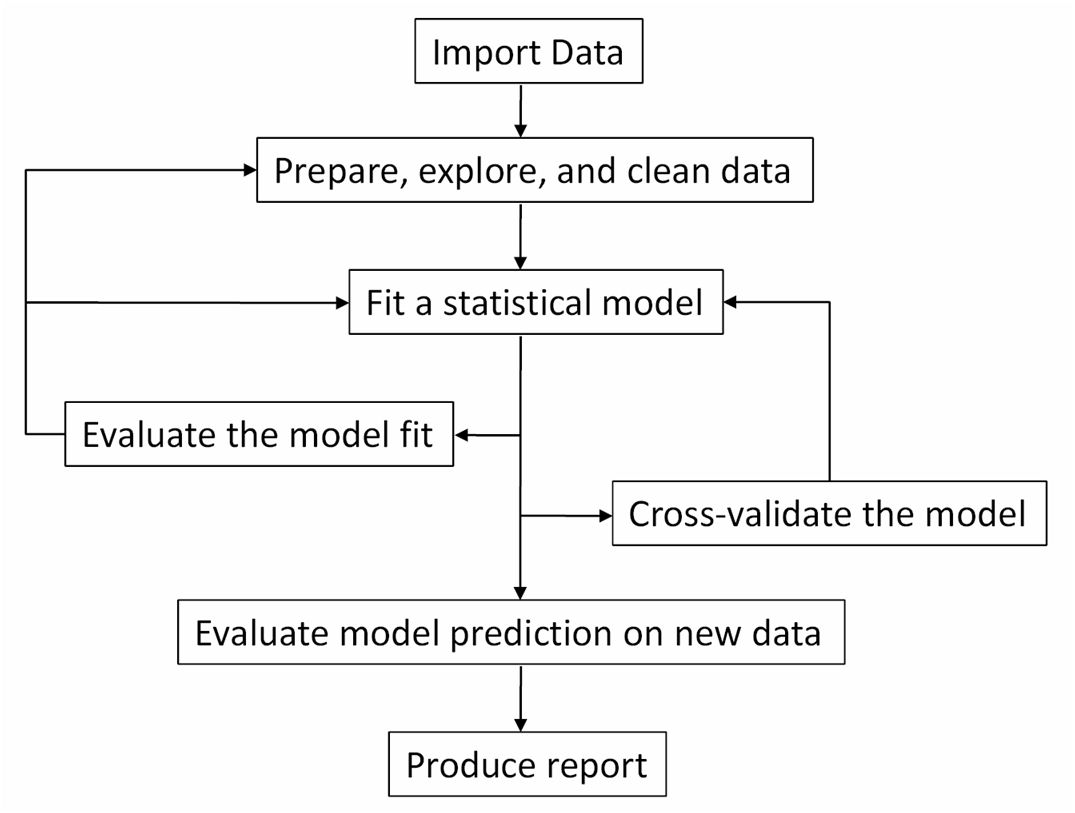
\includegraphics[width=.65\textwidth]{Fig_data_analysis_flowchart_Kabacoff.jpg}
 \caption{A general data analysis flowchart by \citet{Kabacoff2011}.} \label{Fig:data_analysis_flowchart_Kabacoff}
 \end{center}
\end{figure}

Logical reasoning is closely connected to statistical reasoning. At the heart of many research papers is some sort of analysis, i.e.\@ the application of robust analytical techniques to data. For example, \citet{Adrienko2005} think that any data analysis can be described by the following five steps:\index{statistical reasoning}

\begin{enumerate}
  \item \emph{formulate questions}
  \item \emph{choose the analysis methods}
  \item \emph{prepare the data for analysis}
  \item \emph{apply the methods to the data}
  \item \emph{interpret and evaluate the results obtained}.
\end{enumerate}

\noindent Some generic analysis techniques used to develop evidence are for example:

\begin{itemize}
  \item disaggregation / analysis ($X$ can be split into $X_a$, $X_b$,$\ldots$),
  \item aggregation / summaries (sum of $X$; standard deviation of $X$),
  \item correlation / regression analysis ($X$ causes changes in $Y$),
  \item time sequence analysis ($X$ decreases after time $t$),
  \item analogy / comparison ($X$ is higher with method A than with method B),
  \item simulation (generate synthetic $X$ assuming model $m$).
\end{itemize}

\noindent And, of course, there are numerous combinations of these techniques.\par

Note also that to run analysis on data only once might not be sufficiently convincing. Probability theory teaches us that one \emph{`draw'} is insignificant, because it can accidentally be any value from the probability distribution. We can only convince people of the validity of our claims if we repeatedly prove them using new data. This could be impractical, as the costs of collecting data are typically the most expensive part of research. A technique that makes it possible to re-run analysis over and over again, even on existing data, is \textbf{cross-validation}\footnote{Cross-validation implies that we randomly split the original data into calibration (model building) and validation (model evaluation) sets to get an unbiased estimate of the model error. Note that it can be repeated many times.}\index{cross-validation}. Cross-validation is now considered to be a standard step in any model evaluation. The challenge is to find a creative way to run it.\par


\section{Figures and tables (generating and editing graphics)}\label{sec:supergraphics}

\begin{quote}
\emph{``Show, don't tell: seeing is believing.''}\footnote{\url{http://rubyonrails.org/screencasts}}
\end{quote}

Figures and tables\index{figures} in an article are your chance to produce original visualizations of concepts or data. An image is said to be worth 1000 words, but to make a high-quality graph or table can take much more time than to write 1000 words. Hence you should start preparing figures in parallel to writing or even before you start writing.\par

Figures in papers (graphics or artwork)\index{artwork} can be of various types:

\begin{description}
  \item[\textbf{Sketches}] \hfill \\
  Sketches are graphical, simplified representations of rough drawings of important points or key elements of a system. \medskip
  \item[\textbf{Flowcharts}] \hfill \\
  Flowcharts visually display processes and their relationships. These can be e.g. processing steps or decision trees. \medskip
  \item[\textbf{Statistical plots}]\index{statistics!plots} \hfill \\
  Statistical plots are standard plots generated as a result of statistical analysis. The most commonly used statistical plots are correlation plots, trend plots, box plots, and histograms. \medskip
  \item[\textbf{Cartographic materials}] \hfill \\
  Any realistic presentation of geographic phenomena is in fact a map, and every map needs to follow basic cartographic principles. \medskip
  \item[\textbf{Photographs or images}]\index{images} \hfill \\
  Many research articles include photographs (visible light) and/or close range or remote sensing images or scans of objects or surfaces.
\end{description}

In principle, each type of graphics requires a special kind of skill and can be evaluated using objective criteria. The worst thing you can do is underestimate the expertise needed to produce high-quality graphics. People study graphic design and typesetting for years, so it's easy to spot the work of an amateur. Maybe the best way to learn how to make convincing graphics is to learn from bad examples. \citet{Wainer1984TAS} provide a number of amusing examples on how to display data badly. Karl W.\@ Broman from the University of Wisconsin-Madison has created a gallery of top 10 \emph{`worst'} graphs\index{worst graphs} (with apologies to the authors), plus a discussion on what's wrong with them and what should have been done in the first instance\footnote{\url{http://www.biostat.wisc.edu/~kbroman/topten\_worstgraphs/}}.  \par

Typical examples of poor graphic design are:

\begin{enumerate}
\renewcommand{\labelenumi}{(\textit{\alph{enumi}})}
  \item too many variables on the same plot
  \item wrongly emphasized features
  \item inappropriate scale
  \item too many lines over a small area (the \emph{`spaghetti-effect'})
  \item mixing serif and sans serif fonts within the same graph
  \item too small / too large font in relation to the size when printed
  \item too thin lines
  \item over-compressed images and graphs converted to too low resolution (e.g.\@ $<$150 DPI)
  \item missing axis labels and units on graphs or 2D plots.
\end{enumerate}

Figures and tables should be easy to understand without reference to the main body of the article. Graphics that are not informative or those that are obvious should be omitted. All abbreviations and symbols, on the other hand, that are not obvious need to be defined in captions or footnotes.\par

Theoretically speaking, the efficiency of the graphics in a paper can be measured by assessing the \textbf{information resolution}\index{information resolution}, expressed as \citep{Tufte1992}:

\begin{equation}\label{E:info.res}
    {\rm information} \; {\rm resolution} = \frac{{\rm bits}}{{\rm time} \times {\rm area}} - {\rm noise}
\end{equation}

Although this parameter is often not assessed for all graphics, it is obvious that the quality of graphics will increase if we produce info-dense graphics (i.e.\@ plots or charts that consist of many information elements) that are still readable and clear.\par

From our experience, producing quality graphics requires adherence to the following guidelines:\index{graphics}

\begin{itemize}
  \item \emph{Sketches} --- Sketches are simplified, symbolic representations of ideas, so make sure you use simplified graphical items and nothing too complex. It's not a good idea to mix sketches with objective representations of reality such as statistical plots, because this can cause confusion --- sketches by definition do not have to reflect true dimensions and ratios. They are only rough illustrations of concepts.
  \item \emph{Flowcharts} --- A typical mistake people make with flowcharts is that they mix them with sketches. Flowcharts need to be complete, i.e.\@ they should not contain any dead ends or decisions that are ambiguous. Imagine transferring a flowchart to an algorithm. If some parts are not complete, then you will not be able to implement them. Flowcharts can best be produced using specialized software such as Microsoft \textsf{Visio} or Open Office Draw.
  \item \emph{Statistical plots} --- Producing statistical plots is a science in itself. The most common mistake authors make is that they either miss out labels or they mismanage graphical elements. Use decimal points (not decimal commas) for real numbers. We recommend you check out the literature, which is extensive. For example the \textsf{R} community has now several textbooks on multivariate \citep{Sarkar2008,Wickham2009} and interactive graphics \citep{Theus2008}. You can also simply browse examples of statistical plots used in \textsf{R}\footnote{\url{http://addictedtor.free.fr}}'\footnote{\url{http://bm2.genes.nig.ac.jp/RGM2/}} and then try to adopt and/or improve them.
  \item \emph{Cartographic materials} --- Maps\index{maps} are often 2D rectangular graphs, but with many specific properties. In order to avoid major misuse of cartographic data, always indicate in the plot or in the text: map source, the effective scale, projection type i.e.\@ coordinate system and map orientation (direction of north). If possible, also indicate mapping accuracy and refer to a URL where there is more technical information (metadata) about the map.
  \item \emph{Photographs or images} --- Photographs\index{photographs} and images are typically easier to import into an article. The key issue is that the resolution of such images should correspond to the rule of thumb 150--600 dots per inch (DPI). This means that if the width of an image in the text is e.g. 8~cm, then the size of image should be at least 450~pix, ideally 900~pix (document distribution), and not more than 1800~pix (press). Also be aware that color images will often need to be converted to gray-scale images in journals. Hence it is a good idea to do this conversion before submitting the article. The way to improve the images even more is to maximize the contrast by using some standard histogram equalization functions implemented in image processing packages such as \textsf{Adobe Illustrator} or \textsf{PaintShop}.
\end{itemize}


The European Association of Science Editors (EASE) emphasizes in their general guidelines\footnote{\url{http://www.ease.org.uk/guidelines/}} that manipulation of images to make a false impression constitutes scientific fraud, so graphical editing of such materials should be taken very seriously.\par

Tufte believes that the best way to learn to make high-quality graphics is to look at the templates used by Nature, Science or other high-impact journals. People who publish in these journals usually have 1.5 pages of space to tell a complex, significant story. Clearly, the graphics that make it into such articles must be the best. Consider, for example, the artwork and graphics used in The Economist, the New York Times and Science Mag. Everything in these plots is high art, right down to the smallest detail. And nothing stops you from learning from the masters. Tufte\index{Tufte}: \emph{``Talent imitates, genius steals!''}\footnote{Edward Tufte at a one-day workshop on presenting data and information held on March 28, 2010, Pittsburg (PA).}\par

Tufte goes beyond standard graphics and suggests the use of so-called \emph{``supergraphics''}\index{supergraphics} --- high-resolution visuals with a high density of information per area (take a look for example at Fig.\@~\ref{Fig:map_of_science}). Such supergraphics impress and inspire people --- they immediately get involved with the topic and start interpreting and analyzing. David McCandless\index{McCandless}, an information designer from London, has dedicated his career to discovering original ways to visualize important information\footnote{\url{http://www.informationisbeautiful.net}}. It is striking how many hidden connections and patterns there are in data we already know. \par

Impressive tabular materials are even more difficult to design and use than artwork. Good table design, for example, is extremely difficult. MS Office or similar text editors will not be of much help. Likewise, journals typically do not provide table templates that you can easily adapt for your data. {\LaTeX}, for example, has several packages that allow production of super-tables (tables that spread over several pages) and allows combination formulas, plots, numbers and text tables\footnote{\url{http://www.macrotex.net/texbooks/}}. By combining {\LaTeX} and \textsf{R} one can produce high-quality scientific graphics that will impress both scientists and wider audiences\index{S--weave}.  \par

Many commercial publishers run automatic checks for Artwork Quality. This, for example, is the result of an artwork quality review of a plot that was produced using \textsf{R} and then exported into PostScript format:

\medskip
\begin{center}
  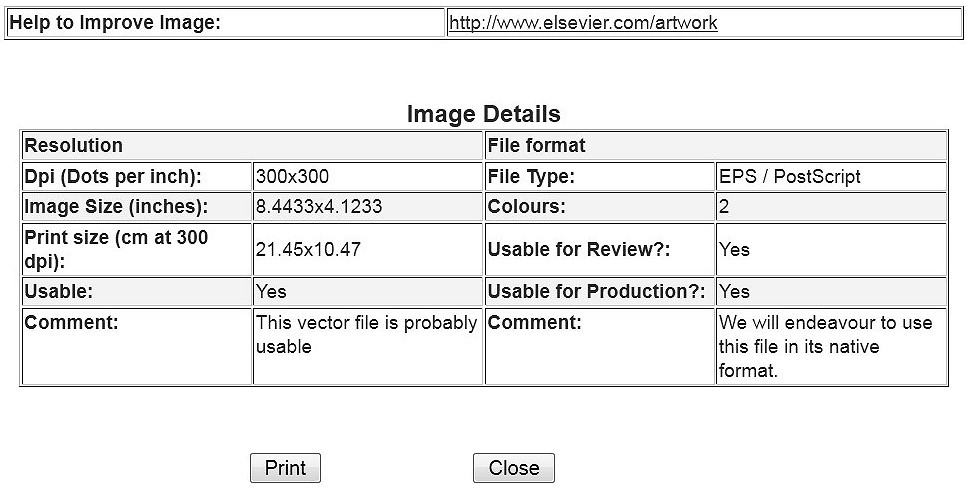
\includegraphics[width=.9\textwidth]{Fig_screen_artwork_check.jpg}
\end{center}

In order to see whether your graphics will really look good in your article you should consider building a PDF with formatting close to the Camera Ready Copy formatting used by the publisher. For example, while writing this book we kept adjusting sizes and widths in {\LaTeX}, which allowed us to find an optimal combination of text and graphics. There are also commercial packages that you can use, such as \textsf{Adobe PageMaker}, \textsf{Microsoft Publisher} and \textsf{Scientific WorkPlace}\index{software!\textsf{Scientific WorkPlace}}. \par


\section{Citing sources}\index{citing!sources}

\begin{quote}
\emph{``The purpose of academic citation is to give credit to those whose work and ideas have shaped your thought, to clearly differentiate between what you have done and what others have done, and to help readers locate the texts/work that has influenced you.''}\footnote{Adapted from the e-mail forum of the Middle East and North Africa Writing Centers Association: \url{http://menawca.org}.}
\end{quote}

Citing literature sources is as important a skill as any other writing skill. The way we cite and what we cite in our work is becoming ever more important because citation statistics are likely to become THE evaluation criterion.\par

According to \citet{Rossiter2010RCS}\index{Rossiter}, an author should aim to cite \emph{the most relevant}, \emph{reliable}, and \emph{accessible} sources only --- \emph{``Superfluous references do not impress; they confuse''} \citep[p.32]{Rossiter2010RCS}. Imagine, for example, that you are using a statistical method that was described 50--60 years ago. Imagine that this method has been published in several formats (e.g.\@ as a part of a PhD thesis, technical report, journal article and book section). Since then it has been reviewed and revisited by several other authors. Then, a summary of the method has been added to an encyclopedia and a website that specializes in this topic. There could many relevant references for this method, so we can easily get lost in figuring out which one to choose (should we cite them all?).\par

According to \citet{Rossiter2010RCS}, there is a logical sequence that everyone should follow when citing sources, approximately:

\begin{itemize}\index{how to cite}
  \item First, try to use the most original peer-reviewed reference published by an international publisher.
  \item If this is not available, then refer to the most original peer-reviewed publication even if it produced is by some local or regional publisher (e.g.\@ via a non-ISI journal).
  \item If this is not available, then refer to the most original publication from a publisher or academic institution, one that has been catalogued via the WorldCat (i.e.\@ which at least has an ISBN and/or a catalogue number).
  \item If the only source is unedited conference proceedings, refer to the volume title, conference location and/or hosting institution and URL.
  \item If this is not available, then at least refer to the most original publication that is accessible via an URL (e.g.\@ an on-line report or a PDF).
  \item If no other publication is available, but only a cross-reference to a review article, encyclopedia article or newspaper article, then refer to the document so that anybody can find the same source within a period of at least the next five years (if necessary put a PDF online and refer to a permanent URL).
\end{itemize}

Referring to encyclopedias or lectures notes is not acceptable to most journals. Encyclopedias are only reviews or resumes of topics and hence by definition are not meant to provide new information. If they leave out a reference to the original publication (which is very common), you might get a wrong impression that this is THE source. It rarely is. Likewise, lecture notes are usually written for internal purposes and often create the wrong impression (that the authors are producing something original).\par

\begin{svgraybox}
The purpose of academic citation is to give credit where it is due, place the paper in the network of papers and researchers on the topic, and provide documentary evidence for the statements made in your paper.
\end{svgraybox}\label{R:citations}

Many academics rush to put things on the web without a second thought. Big IT companies such as Google or Microsoft \emph{crawl} over www and archive all the content that appears on-line. This content is then available via their cache, which is still on-line even if you decide to remove your PDF from the web\footnote{You can remove some of the Google cached content by logging in to the \url{http://www.google.com/webmasters/tools/removals}\index{Google, removal tool}, but this is not a trivial issue.}. Once you put things on the web for a few days and allow public access --- it stays there forever, so think twice before you click that upload button!  \par

Many materials finish up on the web without much filtering and cross-checking. As a rule of thumb, at least half of the content you find on the web contains errors, is outdated or inaccurate (sometimes even on purpose). Commercial publishers, public agencies and academic institutions can at least certify with their name that the published content has gone through some kind of filtering process, although there is almost never any warranty that the information in publications is 100\% correct (even nicely formatted articles can contain a lot of nonsense). \par

Here's a list of some common misconceptions about who and how to cite:

\begin{itemize}\index{citing!misconceptions}
  \item Citing literature is in general a good thing\footnote{Some investigations have shown that papers with more references have a slightly higher impact.}, but putting in hundreds of irrelevant citations is counter-productive. \citet{Smith1990TR}, for example, suggests that authors should limit their list to contemporary, relevant and essential references only: \emph{``The purpose of academic citation isn't to show that you are a `good student' who has read everything on a subject and can't see the forest for the trees.''}
  \item Citing \emph{sexy} papers doesn't mean that yours will become one.
  \item Citing the work of reviewers (or supervisors) can please them, but if they are fair reviewers than they will not be impressed. If their vanity is overwhelming, then you should maybe rethink publishing in that journal.
  \item Although it seems easier to cite review articles than to read all of the original publications (it saves you a lot of homework), you should always try to dig into the literature --- detective work can be fun!
\end{itemize}

\begin{figure*}[!htb]
\begin{center}
  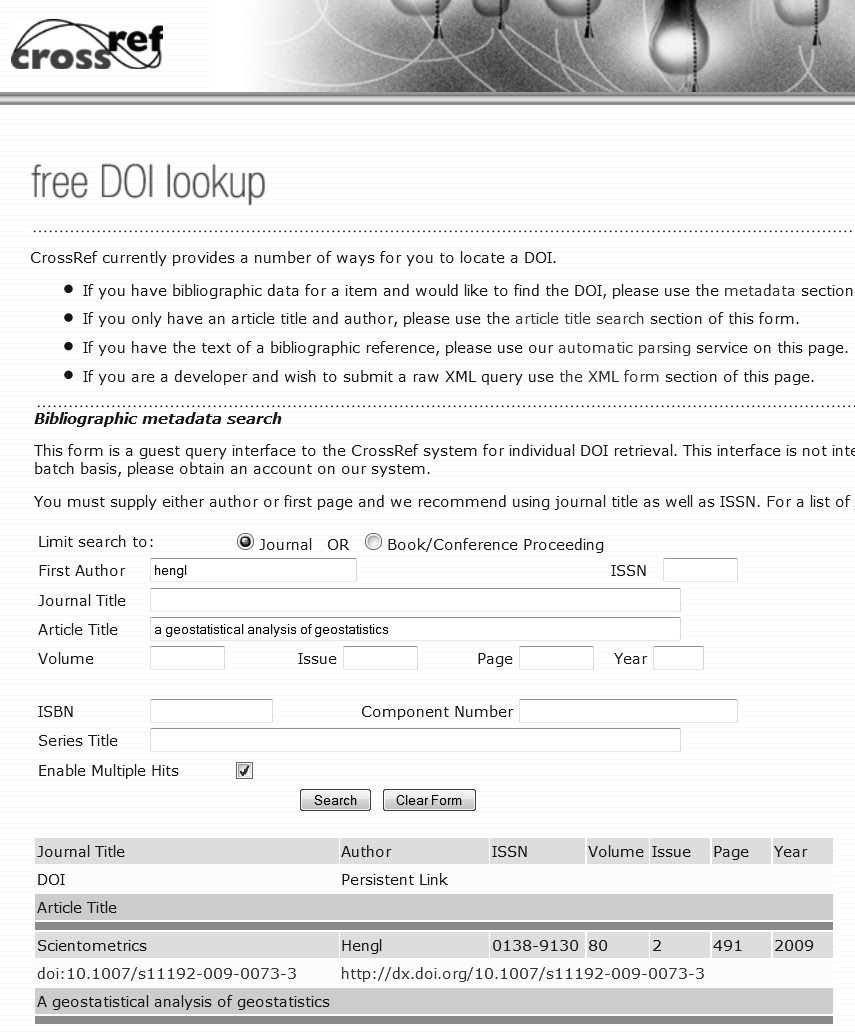
\includegraphics[width=\textwidth]{Fig_crossref_search_screen.jpg}
\caption{CrossRef.org portal provides a free DOI lookup\index{DOI lookup}\index{references, import} service where you can find unique identifiers using first author and title. Once you have a DOI or ISBN, you can easily import a reference to your document (BibTeX or EndNote\index{EndNote} format) and avoid any additional work and typing errors.} \label{Fig:crossref_search_screen}
\end{center}
\end{figure*}

Ideally, you should refer not only to publication records, but also to page or table/figure numbers. Imagine that someone really wants to check your numbers or claims --- wouldn't you like to help them find the source quickly? Imagine you refer to some results (numbers, plots) published in a thick monograph. How much time would it take to find that specific fact? Hours? Days? In fact, it's highly probable that in the near future publishers will cross-link the references to URL repositories of documents. We will then be able to refer to \emph{micro-location} of a cited source. For example, something like this:\index{citing!sources}

\begin{itemize}
  \item Books $\mapsto$ \texttt{ISBN:Page:Line}
  \item Journal articles $\mapsto$ \texttt{DOI:Page:Line}
  \item Newspapers and daily journals $\mapsto$ \texttt{ISSN:Date:Page:Line}
  \item Video materials $\mapsto$ \texttt{OCLC:Minute}
  \item Web-materials $\mapsto$ \texttt{IP:Anchor:Date}
\end{itemize}

Google has been pushing a project\footnote{\url{http://books.google.com/googlebooks/library.html}; other similar competing projects are \url{http://europeana.eu}: the European archive of digital libraries, and \url{http://www.hathitrust.org}: the digital archive of USA University libraries.} to scan all (!) of the books in the world and index them (which they have done efficiently with many other types of information) so that a micro-reference to a page in a book or article would take you directly to the specific section or paragraph. References will then probably become redundant and we will only need to refer to a unique ID (Fig.\@~\ref{Fig:crossref_search_screen}). In the meantime, it might be a good idea to scan pages with important reference sources and share them among your co-authors, just to improve the collaborative writing process.\par

References tells a lot about the article --- the way we cite and the length of references determines the quality of the research we produce. Here two rules apply. First, read more and you will start to cite more and consequently minimize the chance that you will miss an important reference. Remember that articles that cite more references are in turn cited (slightly) more themselves \citep{Webster2009}. Second, be critical about what you read. If in doubt, cite only the work that is relevant, accurate and significant, or as \citet{Corbyn2010} puts it: \emph{``to be the best, cite the best''}.\par


 \section{The art of line editing}\index{line editing}

\begin{quote}
    \emph{``Learn to enjoy the tidying process. I don't like to write; I like to have written. But I love to rewrite. I especially like to cut: to press the DELETE key and see an unnecessary word or phrase or sentence vanish into the electricity$\ldots$ with every small refinement I feel that I'm coming nearer to where I would like to arrive, and when I finally get there I know that it was the rewriting, not the writing, that won the game.''}\footnote{Willem Zinsser in \emph{``On Writing Well''}.}
\end{quote}

Once you are sure that you and your co-authors are satisfied with the macro (sections) and meso (paragraphs) structure of your article, it's time to zoom further into the paper and analyze the article sentence by sentence. The key to improving the microstructure of a paper is to compress sentences, improve the balance of foreground and background information, and make links between short, \emph{staccato} sentences. This is \emph{``the art of line editing''}.\par

Here are some general strategies:

\begin{itemize}\index{redundant words}
    \item \emph{Compress sentences} by reducing unnecessary or redundant words. Instead of writing \emph{``a considerable number of''} use \emph{``many''}; instead of \emph{``this result would seem to indicate''} use \emph{``this indicates}''. Omit obvious sentences such as: \emph{``It is well known that$\ldots$ }'' and  \emph{``The correlation plot is shown in Fig$\ldots$ }''. However, be careful not to overdo the use of short sentences --- \citet{Jasper2002CC}: \emph{``Every sentence cannot be urgent. Good writing normally requires a combination of longer and shorter sentences, carefully orchestrated in each paragraph.''}
    \item \emph{Split long, heavy sentence} into two or even three. Keep paragraphs short and eye-catching. Zinsser\index{Zinsser}: \emph{``Short paragraphs put air around what you write and make it look inviting.''}\index{paragraphs}
    \item \emph{Improve the flow}: at the beginning of a sentence put old information that links back to the previous one and, at the end, put the new information you want readers to focus on. In English, the steps in an argument tend to be built up progressively in coherent paragraphs, with each step linked to the one before, usually through sentence subjects. Example: \emph{``The use of land, water and minerals has increased more than tenfold during the past two centuries $\mapsto$ Future increases in population and economic development will intensify this pressure $\mapsto$ The cumulative impacts of human activities are likely to lead to major environmental changes, varying from disruption of local ecosystems to disturbance of the biosphere.''}
    \item \emph{Use linking words} such as \emph{although}, \emph{as is clear from}, \emph{as a result of which}, \emph{but}, \emph{most of which}, \emph{or}, \emph{so}, gerund forms (\emph{using\ldots  requiring}), \emph{while}, \emph{which is why}, \emph{which indicates that}, \emph{when}, \emph{where}, and \emph{yet}. This approach improves `message management' by arranging information to show what is important, grouping related ideas, and highlighting the relationships between different parts of the argument. It enhances readability, allows variation in sentence length, and avoids redundancy.
    \item If too much information is placed at the front of the sentence (\emph{frontal overload}) and too little at the end, the rhythm of the sentence is disturbed and it becomes more difficult for many readers to process the information. Instead of writing: \emph{``Working with students is what attracts me most in this job''} write: \emph{``What attracts me most in this job is working with students.''}
    \item Putting \emph{information in the middle} of a sentence may disturb the flow and can lead to the wrong elements (e.g.\@ pronouns) being stressed, or to redundancy. English readers are unused to the verb coming at the end of a sentence. They process information as they go along. For example, avoid writing: \emph{``It is for the purpose of the present study convenient to$\ldots$ ''}.
\end{itemize}

As \citet{Gopen2004} points out in \emph{``Expectations: Teaching Writing from the Reader's Perspective''}, when trying to understand a sentence, readers need to find the answers to five important questions:

\begin{enumerate}
  \item \emph{What's going on here?}
  \item \emph{Whose story is it?}
  \item \emph{What is the most important piece of information in this sentence?}
  \item \emph{How does this sentence link backwards to the one that precedes it?}
  \item \emph{How does this sentence lean forwards to the one that follows it?}
\end{enumerate}

\begin{flushleft}
\textbf{Cutting things out}
\end{flushleft}

\noindent One efficient way to improve coherence is to re-read paragraphs from the beginning and then:

\begin{itemize}
  \item reorganize and inserting missing links between paragraphs where necessary
  \item delete redundant content
  \item improve the connection between sentences (all sentences within a paragraph should be logically connected; otherwise make new paragraphs)
  \item compress long, over-complex, ambiguous sentences using normal everyday language.
\end{itemize}

In his general guide to writing, \citet{Zinsser2006} suggests that in most drafts 50\% of the content can be cut out without losing the author's voice.\index{Zinsser} \citet{Zinsser2006} further suggests that the key to improving the value of a manuscript is in decreasing the \emph{`clutter'}\footnote{According to the Cluetrain Manifesto (\url{http://www.cluetrain.com}),  \emph{``business babble''} is the types of language used by corporations to hide their mistakes.} --- \emph{``fighting clutter is like fighting weeds''}. To cut things out, however, requires skill. Zinsser: \emph{``If you give me an eight-page article and I tell you to cut it to four pages, you'll howl and say it can't be done. Then you'll go home and do it, and it will be much better. After that comes the hard part: cutting it to three.''} \par

If in doubt, cut it out. \citet{Creedy2008research} puts it like this: \emph{``Some well-chosen cuts can reduce the length while at the same time improving the flow of a sentence.''} Some editors suggest that in most papers submitted to journals, it's possible to omit the first paragraph without serious loss of meaning \citep{Creedy2008research}. There's no need to tell your audience things they already know. There's also no need to use empty verbs (see examples below) that overload sentences and irritate readers. A must read for anyone that wants to develop skill in reducing noise in your documents is \citet{dupre1998bugs}.\par

Correct specialist terminology is clearly essential in scientific writing, but you should use the words and patterns of normal, everyday language to link scientific terms and concepts. Beware of pseudo-scientific \emph{`empty'} verbs. Below are some examples\footnote{These examples were collected by academic writing teacher David Alexander.} of correct and incorrect uses of \emph{``observed''} and \emph{``showed''}:

\begin{flushleft}
\textbf{Potentially empty verbs: \emph{`observed'}}\index{empty verbs}
\end{flushleft}

\begin{enumerate}
  \item Original sentence (from a review):
    \begin{quote}
    \emph{``These differences are for a large part caused by the different modeling methods observed, with differences in time horizon as one of the most prominent causes.''}
  \end{quote}
  Is \emph{`observed'} necessary here? No.
  \begin{quote}
  \emph{``These differences were caused largely by different modeling methods, with differences in time horizon as one of the most prominent causes.''}
  \end{quote}
  \item Original sentence:
    \begin{quote}
    \emph{``Apart from these essential differences on time horizon, large differences between modeling methods were observed in general.''}
  \end{quote}
  Is `observed' necessary here? No. Authors have an opinion, but this is not connected to the actual measurements.
  \begin{quote}
  \emph{``As well as these essential differences in terms of the time horizon, there were large overall differences between modeling methods.''}
  \end{quote}
  \item Original sentence:
  \begin{quote}
  \emph{``Tumor regression was observed in 16 selected patients during curative radiotherapy. Patient selection was based on visual tumor regression on cone-beam CT scan without atelectasis.''}
  \end{quote}
  Is 'observed' necessary here? Not if the writer means this:
  \begin{quote}
  \emph{``Tumors regressed in 16 selected patients during curative radiotherapy. Patient selection was based on visual tumor regression on cone-beam CT scan without atelectasis.''}
  \end{quote}
  But she actually meant this:
  \begin{quote}
  \emph{``To observe (the process of) tumor regression during radiotherapy, we selected 16 patients on the basis of visual tumor regression on cone-beam CT scan without atelectasis.''}
  \end{quote}
  \item Original sentence:
  \begin{quote}
    \emph{``This raises questions with regard to microscopic pathological response, which cannot be observed on CT-scans.''}
  \end{quote}
  Is `observed' necessary here? Yes.
\end{enumerate}

\begin{flushleft}
\textbf{Potentially empty verbs: \emph{`show'}}
\end{flushleft}

\begin{enumerate}
  \item Original sentence:
  \begin{quote}
    \emph{``The model showed that the throughput time of the diagnostic track could be reduced from 21 to 5 working days with 18 mins of idle time per day \& 10 minutes of overtime per day.''}
  \end{quote}
  Is \emph{`showed'} necessary here? Yes --- the model demonstrated something, which is what models are designed to do.
  \smallskip
  \item Original sentence:
  \begin{quote}
    \emph{``We show that neither the combined expression of TTFCE6SH and TTFCE7SH nor the combination of one of the shuffled genes with its WT counterpart enabled transfected NIH 3T3 cells to form colonies in soft agar.''}
  \end{quote}
  Is \emph{`show'} necessary here? Yes, science readers expect other researchers to show them things.
  \smallskip
  \item Original sentence:
  \begin{quote}
    \emph{``The best results were obtained with a 1/9/1 w/w ternary mixture of docetaxel, polyvinylpyrrolidone (PVP)-K30 and sodium dodecyl sulphate (SDS) which showed a significant increase in rate and extent of in-vitro dissolution of docetaxel.''}
  \end{quote}
  Is \emph{`showed'} necessary here? Not if the writer means to tell us something like this:
  \begin{quote}
    \emph{``The best results were obtained with a 1/9/1 w/w ternary mixture of docetaxel, polyvinylpyrrolidone (PVP)-K30 and sodium dodecyl sulphate (SDS), which significantly increased the rate and extent of in-vitro dissolution of docetaxel.''}
  \end{quote}
  Before writing \emph{`showed'}, ask yourself what actually happened. Here, the main effect of the mixture was to increase something. Much in the same way as genes don't \emph{`show'} expression, but are expressed, mixtures don't usually \emph{`show'} anybody anything.
  \smallskip
 \item Original sentence:
  \begin{quote}
    \emph{``The RING domain structure resembles other U-box/RING domains, but the N-terminal helixes show an interesting asymmetric arrangement, a phenomenon that has not previously been seen in such domains.''}
  \end{quote}
    Is `showed' necessary here? No. \emph{``Are arranged''} is a much more suitable verb:
  \begin{quote}
    \emph{``The RING domain structure resembles other U--box/RING domains, but the N--terminal helixes are arranged asymmetrically, a phenomenon that has not previously been seen in such domains.''}
  \end{quote}
\end{enumerate}

\begin{flushleft}
\textbf{Making strong(er) points}
\end{flushleft}

\noindent At the micro-level, you might want to strengthen (or weaken) your arguments. If you are not a native English speaker, consider using some of the following phrases to build effective arguments:

\begin{itemize}
  \item the objective of this study is to draw a distinction between / make a comparison between$\ldots$
  \item our aim is to raise important questions / take into consideration$\ldots$
  \item we want to make a case for / put greater emphasis on$\ldots$
  \item many studies have attempted to assess the significance of$\ldots$
  \item in study we wish to draw attention to new research which suggests$\ldots$
  \item here we present the case for$\ldots$ / we put forward the argument that$\ldots$
  \item we draw the conclusion that$\ldots$
\end{itemize}

\bigskip
\begin{fminipage}{.9\textwidth}{\footnotesize{\textsf{\textbf{On the use of \emph{however}\index{however}, \emph{therefore}\index{therefore}, \emph{so} and \emph{thus}}} --- In research on what makes texts readable or not scholarly writing ranks the lowest, not just for the content but also for the \emph{`style'} in which it's written \citep{Raymond1993CCC}. A number of textual factors are analyzed: length of sentences, word choice, etc. One factor is the use and placement of linking words\index{linking words} such as \emph{`however'} (as well as thus, therefore, and, but, also, because, and although). Placing these words at the beginning of sentences can help to signal to readers quickly --- without them having to delve --- when the author intends to make a logical connection or shift. However, if it sounds unnatural, it will reduce readability, so the impact may be different on native and non-native speakers of English\index{English!however}. The use of \emph{`however'} and \emph{`thus'} at the beginning of sentences is different in written and spoken English. And written English in the US tends more than British English to mimic spoken English. Why can the connector \emph{`so'} be placed in the initial position, while other connectors are less preferred in that position? Clearly, there is no actual grammatical rule forbidding connectors at the beginning of sentences. And native speakers do use them. So it's not actually wrong. The difference with \emph{`so'} is that a sentence starting with \emph{`so'} flows along quite happily, whereas one that starts with \emph{`thus'} has to come to a stop before it gets started.}}
\end{fminipage}
\bigskip

The following sentences make somewhat weaker arguments:

\begin{itemize}
  \item The data broadly supports the view that$\ldots$
  \item It appears that the effects of $\ldots$ can be explained with$\ldots$
  \item We provide evidence to support the claim that$\ldots$
  \item The results indicate that there is a connection between$\ldots$
\end{itemize}

Some scientists tend to \emph{`hedge'} i.e.\@ use weaker arguments that are justified by their research. In such cases, take a stronger stand and be more assertive about your discoveries and conclusions e.g.:

\begin{itemize}
  \item The results of this study confirm that$\ldots$
  \item This is a clear illustration of$\ldots$
  \item The data does (or does not?) show$\ldots$ and this trend is significant.
  \item We offer proof that$\ldots$
  \item We challenge the theory$\ldots$
\end{itemize}

Of course you don't only need to choose your arguments well. You also need to select facts to focus on. Remember that the most interesting facts are:

\begin{enumerate}
  \item \emph{simple}
  \item \emph{analogous to many other facts}
  \item \emph{grouped with others (i.e.\@ not isolated)}
  \item \emph{those that have a greater chance of recurring}.
\end{enumerate}

How do you choose which facts to emphasize? Select those that possess beauty and harmony. The more general a rule is, the greater its value. The best rules are simple and elegant. Once a rule is established, the exceptions become important. But be prepared to break rules where necessary:\par

\begin{quote}
\emph{``Life is short, Break the rules, Forgive quickly, Kiss slowly, Love truly, Laugh uncontrollably, And never regret anything that made you smile.''}\footnote{Combination of quotes by Robert Doisneau and Amber Deckers.}
\end{quote}



 \section{Common language mistakes}

\begin{quote}
    \emph{``I would never use a long word where a short one would answer the purpose. I know there are professors in this country who `ligate' arteries. Other surgeons tie them, and it stops the bleeding just as well.''}\footnote{Oliver Wendell Holmes, Sr.}
\end{quote}

Editors have discovered that many inexperienced authors (especially non-native English speakers) often repeat the same mistakes. Here are some common ones:

 \begin{itemize}
  \item \emph{Active or passive?} --- Note that it may be necessary to use a passive verb to maintain sentence flow. However, wherever possible, use active constructions within sentences (e.g.\@ write \emph{``This programme focuses on\ldots ''}, not \emph{``The programme is focused on\ldots }''). \emph{``The difference between an active verb style and a passive-verb style --- in clarity and vigor --- is the difference between life and death for a writer''} \citep{Zinsser2006}.
 \item \emph{He or she?} --- Use plural forms to avoid sexist writing. Instead of \emph{``\ldots this affects the end-user, unless `he' possesses\ldots''} $\mapsto$  \emph{``end-users\ldots unless `they' possess\ldots }''. If this solution doesn't work, use \emph{``he or she''} / \emph{``his or her''}.
 \item \emph{Color or colour?} --- Use either UK or US spelling\index{English!spelling} and use it consistently. Follow the spelling in the Oxford Advanced Learner's Dictionary of English (for instance: analyse, honour, colour, realize, organize, programme, centre) or use the US Websters dictionary. Words in a title or a heading should be written in lower case, except for the first word and any proper nouns such as names of persons, organizations or countries, if you use UK style. In US heading style all keywords are capitalized.
 \item \emph{To measure or to make a measurement of?} --- Wherever possible use verbs, not heavy, abstract nouns (e.g.\@ write \emph{``reduce}'' rather than \emph{``achieve a reduction''}). Nouns make sentences stand still. Verbs make them move and push our meaning across to readers. Turning verbs into nouns hides their action. Use \emph{``adapting to''} instead of \emph{``the adaptation to''}; \emph{``for measuring''} instead of \emph{``for the measurement of''}; a project \emph{``designed to develop''} instead of \emph{``aiming at the development of \ldots }''.
 \item \emph{Tripoli or Tarablus} --- Foreign terms for which there are no widely accepted English equivalents should be used with an English translation (in brackets) the first time they  appear. Spell all foreign words correctly and pay special attention to diacritical accent marks such as \`{e}, \'{e}, \"{a}, \"{o} and \"{u}.
 \item \emph{NGO or ngo?} --- Abbreviations must be capitalized. If they can be made plural, this should be done by adding a lower-case ``s'' without an apostrophe. For instance: NGOs rather than ngo's. Spell out terms that are subsequently abbreviated when you use them for the first time, with the abbreviation between parentheses. For instance: Organization for Economic Cooperation and Development (OECD).
 \item \emph{Europe or europe?} --- Geographical terms commonly accepted as proper names are capitalized. Terms are not capitalized when they denote simply direction or compass points. For instance: The Middle East, but western, central and eastern Europe. For the names of newspapers, periodicals and organizations, official titles, and the like use the original spellings (with English translations in parentheses where necessary).
 \item \emph{Hyphenation or hy-phe-na-ti-on?} --- Hyphenation should always break at syllable boundaries. In reports, leave a blank line between paragraphs and do not indent at the beginning of a new paragraph. Avoid a single line of text at the top or bottom of a page (known as `widows' and `orphans').
 \item \emph{Dot or comma?} --- Use the comma (,) rather than the full stop (.) in numbers containing more than four digits (for example: 10,000). Be consistent in your use of currency symbols. These symbols precede the amount of money. Use the euro sign ({\euro}); do not use the words euro or euros. Other currencies should be treated similarly. If you need to refer to American dollars, use US\$ or USD. Don't leave a space between the currency sign and the amount. For instance: {\euro}10,000 rather than {\euro} 10,000 (or 10.000 euros). Use a full stop rather than a comma for decimal places (e.g.\@ write 4.25, not 4,25). Round currency figures off to the nearest euro (or other currency). For instance: {\euro}10,234.59 must be written as {\euro}10,235. Numbers below 10 are usually written in full when used in running text (one, two, three\ldots  nine) unless the sentence contains a combination of numbers. For instance: \emph{``Nine delegates attended the meeting. The 9 delegates represented 18 organizations}.''
 \item \emph{A small number of or a few?} --- Avoid using long-winded expression: find a shorter alternative, e.g.\@ replace \emph{``A small number of''} with \emph{``Few''};  \emph{``Despite the fact that''} with \emph{``Although''}; \emph{``In order to''} with \emph{``To''}; \emph{``Has been engaged in a study of''} with \emph{``Has studied''}; \emph{``There is a reason to believe''} or \emph{``It appears that$\ldots$''} with \emph{``I think''}
\end{itemize}

\begin{svgraybox}
What makes papers look bad? It's either bad logic, bad structure, poor graphics (or a complete lack of them), unclear sentences, vague statements, ambiguity$\ldots$ some papers are too long, some are too short; very often they need to be redrafted.
\end{svgraybox}\label{R:success}

\bigskip
\begin{fminipage}{.9\textwidth}{\footnotesize{\textsf{\textbf{On the use of `I'}}\index{English!On the use of I}\index{first person} --- Much discussion has focused on the use of first person in scientific writing \citep{Raymond1993CCC}. Indeed, many editors do not accept any use of first person style, but an increasing number do \citep{Kirkman2001ESE,Kirkman2004S}. A traditional, technical (depersonalized) writing style is still a prerequisite for submitting articles to some  journals. Many scientists feel it sounds egoistic to write in the first person. Recall the rules of science from page~\pageref{F:rules} --- a research article should be objective and unbiased. However, research articles should not be just a chronological narration of work done (see also the EASE guidelines on page~\pageref{sec:EASEguidelines}). If an author has produced some results, and if these are accurate, then we should all come to the same conclusions and hence the use of \emph{``It can be concluded''} is completely legitimate. However, if you write \emph{``It is assumed that\ldots ''}, \emph{``It was decided to\dots ''}, \emph{``Sites were chosen\ldots  ''}, the reader might ask: who assumes?, who decided? --- the author? or his boss? his client? or\ldots  Obviously, if such information is missing, readers may completely misunderstand the paper \citep{Webster2003EJSS}. There are situations when authors need to make a clear distinction between their opinion and the opinion/results of others \citep{Kirkman2001ESE}.}}
\end{fminipage}
\bigskip

\section{Can you please be more specific?}\label{sec:specific}

\begin{quote}
    \emph{``When a man sits with a pretty girl for an hour, it seems like a minute. But let him sit on a hot stove for a minute and it's longer than any hour. That's relativity.''}\footnote{Quote from the abstract of a short paper written by Einstein that appeared in the now defunct Journal of Exothermic Science and Technology (JEST, Vol.\@ 1, No. 9; 1938).}
\end{quote}

Here is an example from the movie Phenomenon\index{Phenomenon, movie}\footnote{Written by Gerald Di Pego; distributed by Touchstone Pictures.} in which an FBI agent runs some intelligent tests on Mr Malley (the `phenomenon' character):

\begin{itemize}\renewcommand{\labelitemi}{$\blacktriangleright$}
  \item FBI agent: \emph{``Answer as quickly as you can. How old is a person born in 1928?''}
  \item Mr Malley: \emph{``Man or woman?''}
  \item FBI agent: \emph{``Why?''}
  \item Mr Malley: \emph{``Specifics, Bob.''}
  \item FBI agent: \emph{``Okay, one more time. How old is a man born in 1928?''}
  \item Mr Malley: \emph{``Still alive?''}
  \item FBI agent: \emph{``If a man is born in 1928, and he's still alive, how old is he?''}
  \item Mr Malley: \emph{``What month?''}
  \item FBI agent: \emph{``If a man was born October 3, 1928, and he's still alive, how old is he?''}
  \item Mr Malley: \emph{``What time?''}
  \item FBI agent: \emph{``10:00.''}
  \item Mr Malley: \emph{``Where?''}
  \item FBI agent: \emph{``Anywhere!''}
  \item Mr Malley: \emph{``Well, let's get specific, Bob. I mean, if the guy's still alive, born in California, October 3, 1928, 10:00 p.m., he's 67 years, 9 months, 22 days, 14 hours and $\ldots$ and 12 minutes. If he was born in New York, he's three hours older now, isn't he?''}
  \item FBI agent: \emph{``How do you do that?''}
\end{itemize}

In this example, Mr Malley asks for more detail because his model of time is highly accurate (minutes) so that a specific location on Earth determines someone's precise age. Researchers also prefer to know such details. From the point of view of spatio-temporal statistics\index{statistics!spatio-temporal reference}, every variable we measure refers to some space-time \emph{`location'}:

\begin{enumerate}
  \item \emph{geographic location} (longitude and latitude or projected $X,Y$ coordinates)
  \item \emph{height above the ground surface} (elevation)
  \item \emph{time of measurement} (year, month, day, hour, minute)
  \item \emph{spatio-temporal support} (size of the blocks of material associated with measurements; time interval of measurement).
\end{enumerate}

Methods developed to analyze such data require spatio-temporal references\index{spatio-temporal reference} to be accurately specified; otherwise no accurate interpretation of the results can be made. Statisticians recommend that any measured variable in environmental sciences should indicate: geographic coordinates (location), applicable vertical dimension\footnote{Orthogonal distance from the surface of the ground.}, a time reference (time interval of measurement), and the size of the sampling blocks (support size).\par

Take the example of currency. To say that something costs 100 dollars is certainly ambiguous. First, which dollars are you referring to? American, Canadian, Australian$\ldots$ The currency of any dollar is subject to daily fluctuations. For example, 1~US\$ was worth the 0.60~EUR in June 2009, but six months later it was worth 0.825~EUR, and in August 2011 it was worth 0.70~EUR\footnote{See \url{http://www.google.com/finance?q=EURUSD}}. \par

Another issue connected with being more specific about data and results is the applicability scale. Researchers are usually biased in the sense that they take a small sample of the whole population and then, based on such limited results, try to build universal theories. According to \citet{Siegfried2010SN}, statistical tests are widely misunderstood and frequently misinterpreted. As a result, countless conclusions in the scientific literature are erroneous, contradictory and/or confusing. To avoid such criticism of your paper you should:\index{how to be more specific?}

\begin{itemize}
  \item \emph{Always make conclusions that relate specifically to your results}.
  \item \emph{Do not claim new knowledge without evidence.}
  \item \emph{Always refer to statistical significance} and specify: (1) how representative is your sample? and (2) how significant is the difference from random effects?\index{statistics!significance}
  \item \emph{Always indicate the space-time reference} to which the results are applicable.
  \item \emph{Always assume that measurements are `noisy', that uncertainty gets magnified, and that results may be `positive' because of human desire to produce `positive results'}.
\end{itemize}

Unfortunately, we're all biased when it comes to our own work and this bias is not easy to remove.\index{personal bias} As \citet{Creedy2008research} puts it: \emph{``Where subjective judgements are involved concerning the value of work, it is possible that the same filter prevents some useful material from being published, or being published in the most appropriate form.''} Blaise Pascal: \emph{``It is man's natural sickness to believe that he possesses the Truth.''} Donald Kennedy, the editor of Science, also points out that \emph{``scientists often come to believe so strongly in the validity of their theories that they cease to examine them objectively''}\footnote{Published in The Economist, 19 May 2001.}. The first step toward reducing bias in one's work is to acknowledge that it exists.\par


\section{On styles}\index{how to develop a style}

\begin{quote}
\emph{``Good writing does not come naturally, though most people seem to think it does$\ldots$ Writing is hard work. A clear sentence is no accident. Very few sentences come out right the first time, or even the third time. Remember this in moments of despair. If you find that writing is hard, it's because it IS hard.''}\footnote{William Zinsser in \emph{``On writing well''}.}
\end{quote}

For \citet{Zinsser2006} four essential spices of good writing are confidence, enjoyment, intention and integrity. Once you incorporate these successfully, people might get so impressed that they start to recognize you based on your writing. Originality is the highest form of intellectual creation. \par

How do you create your own style of writing? A distinctive writing style often comes through richness of phrases, expressions, and idiosyncratic use of language. Read authors who inspire you, imitate or extend them, then find your own voice. For example, if you're interested in learning how to write in ordinary everyday language that's accessible to both scientists and non-scientists, you could read Richard Dawkin's book \emph{``The selfish gene''} and/or Bill Bryson's \emph{``A Short History of Nearly Everything''}. However, avoid the trap of literally copying sentences from other writers --- be yourself, be relaxed and confident. \par

Also consider acquiring some general writing style guides such as the Chicago Manual of Style and/or the Oxford Style Manual. Some useful style manuals are even available free of charge\footnote{See the MHRA style guide (\url{http://style.mhra.org.uk}), for writing in the arts and humanities.}. There is even a manual from the \emph{``For dummies''} series on how to write research papers \citep{woods2002research}. It should not surprise you that these books are thick volumes because scientific writing is rather exact. \par

The best writers in the world are also the best readers. It is even better if you do some peer review work yourself. Refereeing is a good way to learn to write better papers. \citet{Smith1990TR}: \emph{``evaluating the work of others gives one insight into one's own.''}\par

Another thing you might consider is to think up original expressions that epitomize your work (these are known as \emph{streamers} or \emph{callouts}). One day, somebody might remember you for this.\par

\bigskip
\begin{fminipage}{.9\textwidth}{\footnotesize{\textsf{\textbf{Why is it important to write science using everyday language?}}\index{scientific!writing style} --- For many critical readers, academic writing is a stereotyped joke --- a museum of passive voice, obscure and dull jargon, and stilted paragraphs --- without excitement or entanglement \citep{Jasper2002CC,Webster2003EJSS}. Early in their careers, most academics develop the idea that editors are impressed by a \emph{`dense'} writing style with heavy abstract nouns instead of lively active verbs. Researchers should use specialist terminology, but link it with everyday language to captivate an audience that is intelligent but does not necessarily know much about the topic. We recommend using the language of everyday speech --- not that of spokesmen, lawyers and bureaucrats --- to link scientific concepts. For example, use words with an Anglo-Saxon base to link scientific terms, which usually have a Latin/French origin. Fortunately, much scientific and technical writing in recent years has moved strongly in the direction of spoken English --- shorter sentences and more direct, plain language. Unfortunately, many scientists still erroneously believe they are required to use long, heavy sentences full of abstract nouns.}}
\end{fminipage}
\bigskip

This is what \citet[pp.45--46]{Chomsky2002entretiens}\index{Chomsky} say about how academics write: \emph{``Intellectuals have a problem: they have to justify their existence. Now, there are few things about the world that are understood. Most of the things that are understood, except perhaps in certain areas of physics, can be explained with very simple words and in very short sentences. But if you do that, you don't become famous, you don't get a job, people don't revere your writing. There's a challenge there for intellectuals to take: to take what is rather simple and make it appear to be something very complicated and very profound. Groups of intellectuals interact that way. They speak amongst each other, and the rest of the world is supposed to admire them, treat them with respect, etc. But translate what they are saying into simple language and you'll often find either nothing at all or truisms, or absurdities.''}, which is what Jorge Cham's did with his thesaurus of common academic phrases (deciphering academese):\index{academese}

\begin{flushleft}
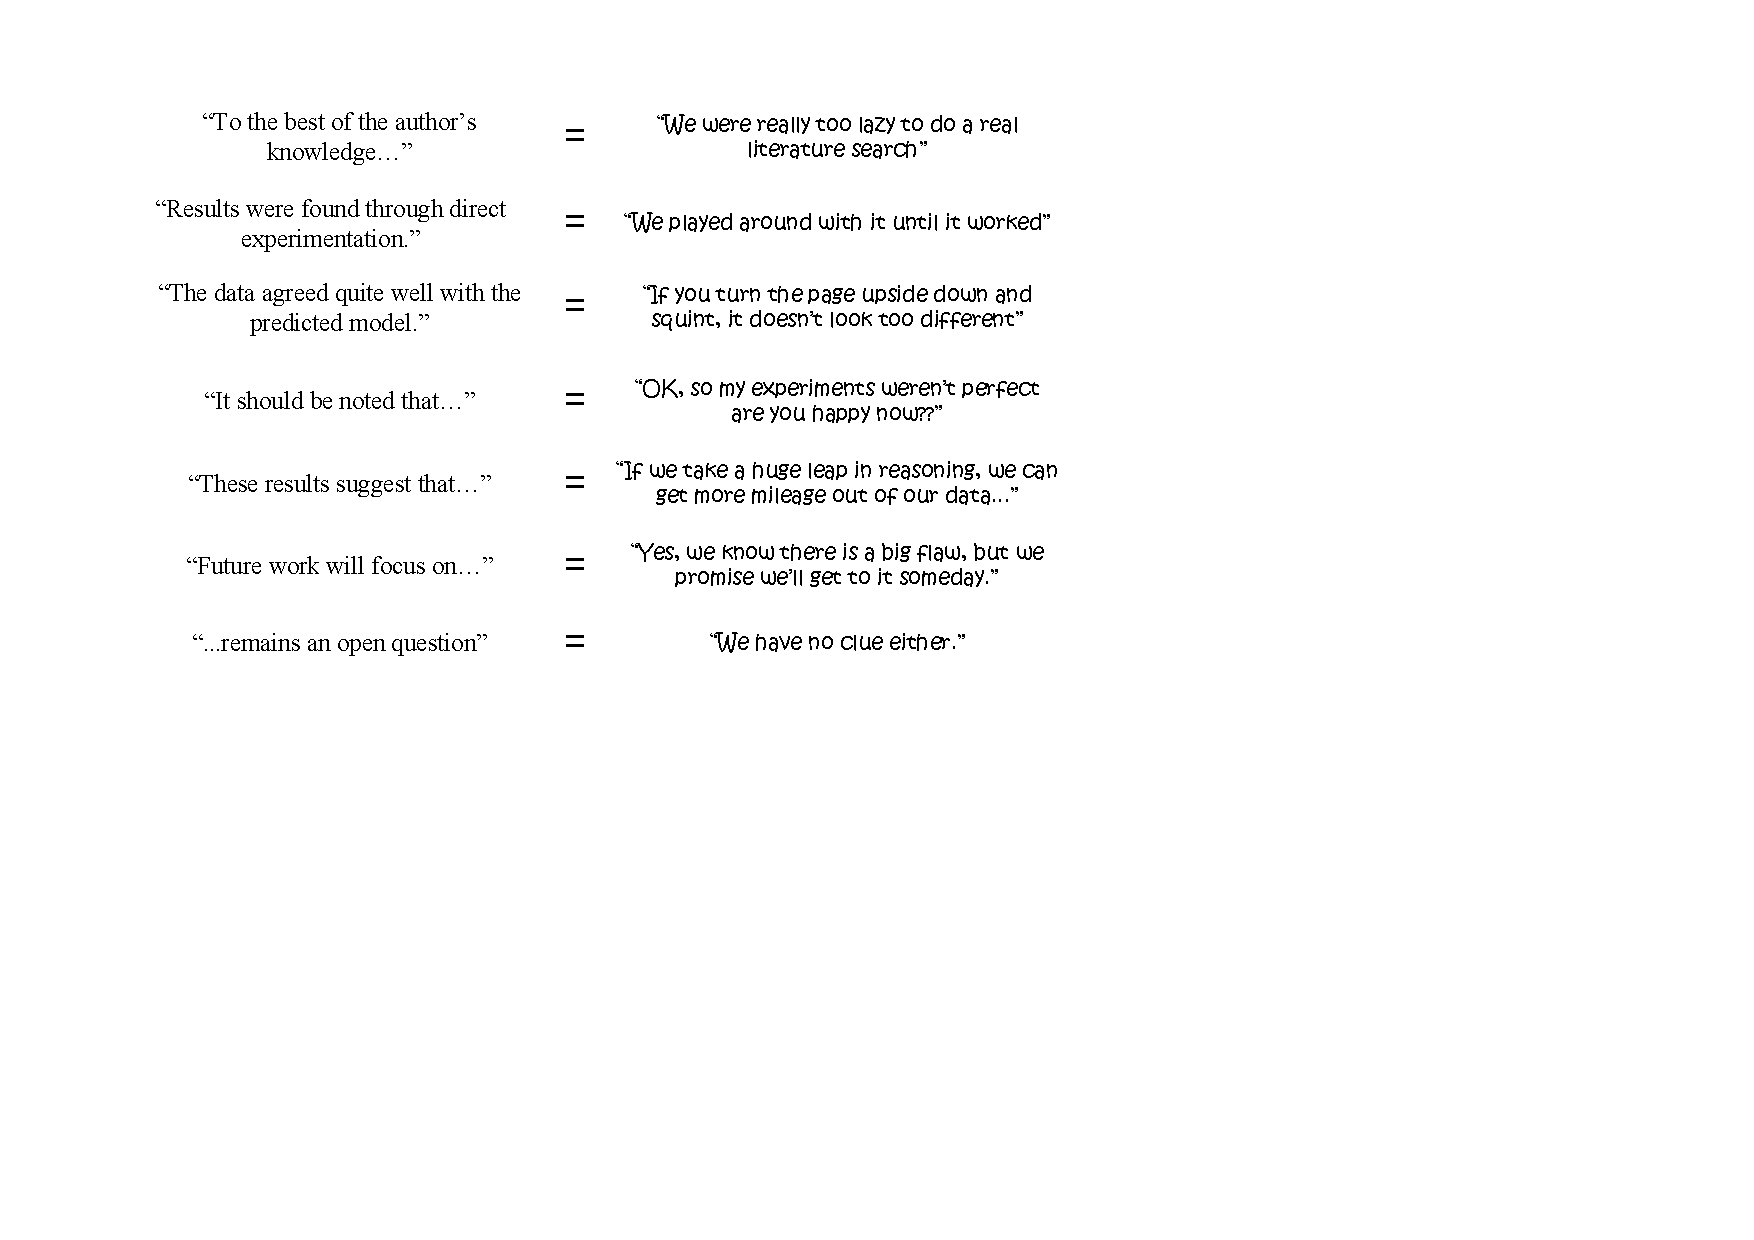
\includegraphics[width=\textwidth]{Fig_academese.pdf}
\end{flushleft}


\section{Collaborative writing}\index{collaboration!editing}

\begin{quote}
    \emph{``Wikipedia is about the power of people like us to do extraordinary things. People like us write Wikipedia, one word at a time. People like us fund it, one donation at a time. It's proof of our collective potential to change the world.''}\footnote{Jimmy Wales, Founder of Wikipedia.}
\end{quote}

Collaborative writing is writing in parallel i.e.\@ more than one person writing in a single copy of a document. Collaborative platforms can be used to generate (1) operational plans (\emph{collaborative planning}), (2) documents (\emph{collaborative writing or editing}), and for (3) annotating text. The advantages of collaborative platforms are:

\begin{itemize}
  \item They enhance collaboration because the co-authors can have a fruitful discussion without needing to meet physically.
  \item A significant amount of time can be saved because several people can work on the same document simultaneously. Imagine how much time it takes if you send a document to co-authors by e-mail and then have to wait to receive comments/revisions (from author to author).
  \item Through collaborative writing co-authors motivate each other to continue writing because the document starts growing and evolving faster.
  \item The lead author can track contributions from all co-authors and then rank them in the author list.
\end{itemize}

Collaborative planning (brainstorming; designing) precedes collaborative writing and editing. We recommend that these activities should be separated. In other words, one should not start writing papers in a group before agreeing about roles and responsibilities. \textbf{Collaborative editing}\index{editing|see{collaboration}} comes later. Although some discussion is still welcome at this stage, it is generally better to agree with your co-authors about the main research questions, the target journal, list of authors and their responsibilities (paper production politics) before editing starts. \par

\begin{center}
  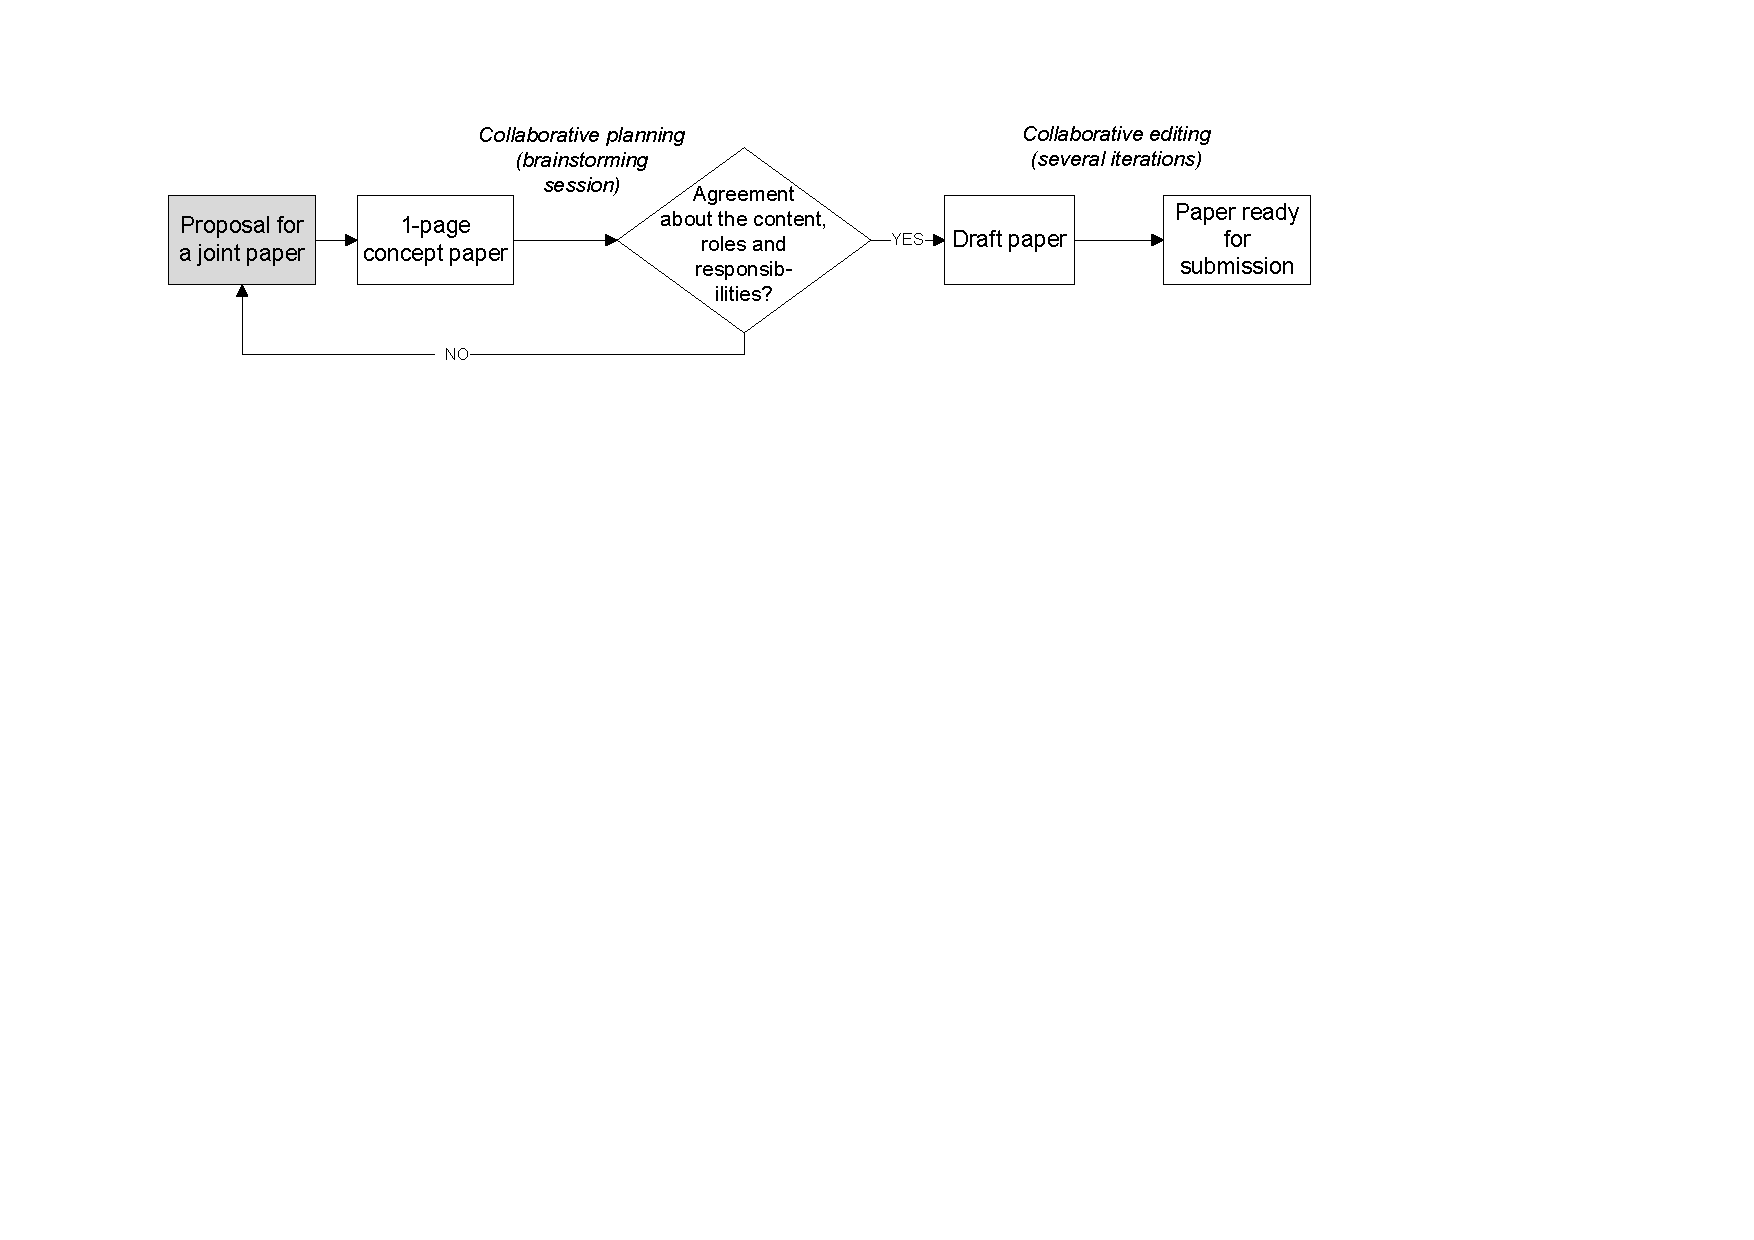
\includegraphics[width=\textwidth]{Fig_collaborative_editing_phases.pdf}
\end{center}

A collaborative editor is a software application that allows several people to edit a computer file using different computers. Editing can be done both in real time and off-line. In both cases the most important thing about collaborative editing is that the there is a single copy of the document that is accessible by a number of users who all have editing rights and can continuously follow the progress of the paper. Another important feature of collaborative editing is that it allows tracking of changes by author and dates.\par

\begin{figure*}[!htb]
\begin{center}
  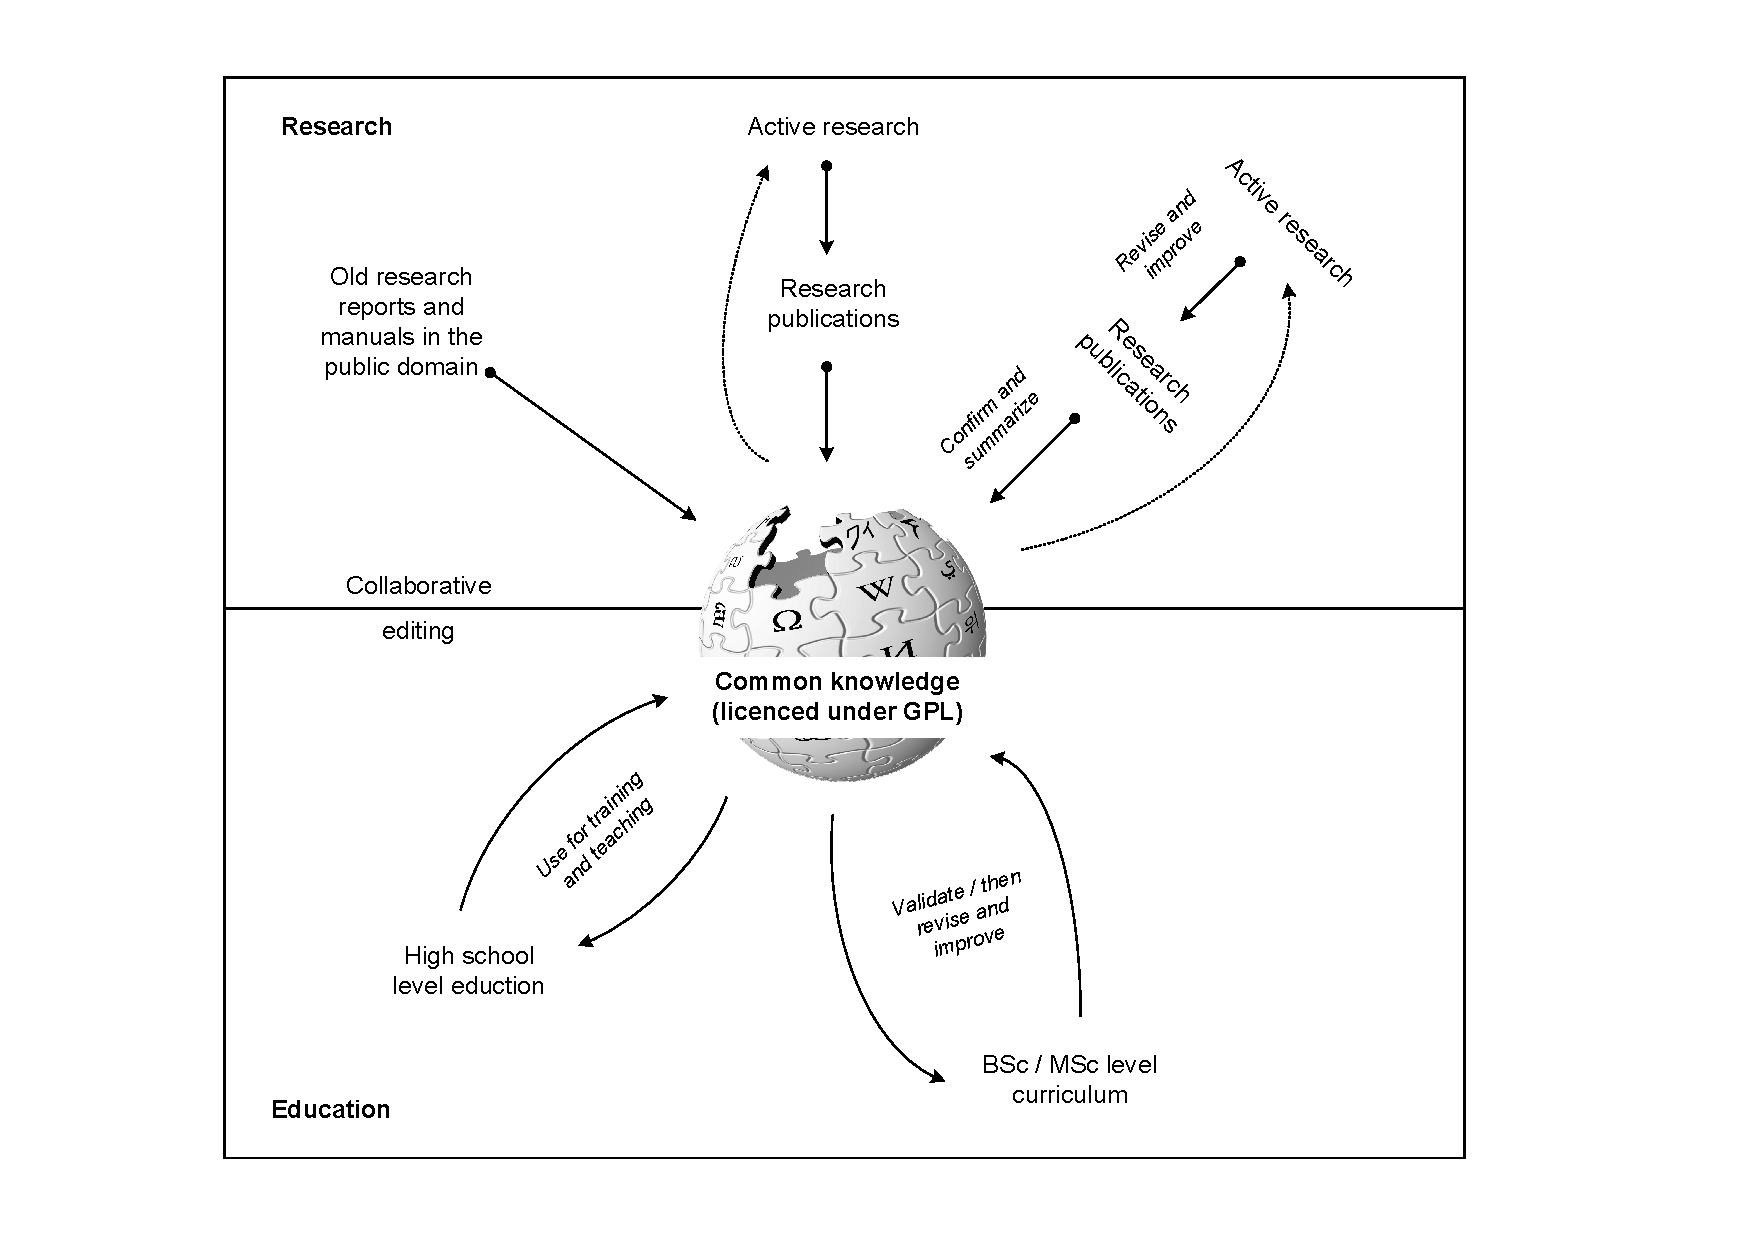
\includegraphics[width=.95\textwidth]{Fig_from_active_research_to_wikipedia.pdf}
\caption{Academic institutions should motivate researchers to contribute content, i.e.\@ the results of their research, to \textsc{Wikipedia} --- the public encyclopedia. \textsc{Wikipedia} is among the top five most visited websites in the world, along with Google, Facebook, Youtube,and MSN. The budget of the Wikimedia foundation\index{Wikimedia foundation} for 2010 was about 20~million US\$; by comparison Google's total costs \& expenses for 2010 were approx.\@ 15~billion US\$ (or 750 times more).} \label{Fig:From_active_research_to_Wikipedia}
\end{center}
\end{figure*}


Real-time collaborative editing can be best achieved by using web-based editors such as e.g.\@ \textsf{Google Docs}, \textsf{Adobe Buzzword}\footnote{\url{http://www.buzzword.com}} or a web installation of \textsf{MediaWiki}\footnote{\url{http://www.mediawiki.org}}. There are also a number of desktop packages for collaborative editing, the most popular of which are Microsoft \textsf{SharePoint}, \textsf{GNU Emacs} and \textsf{Gobby}\footnote{\url{http://gobby.0x539.de}}.\par

\textsc{Wikipedia}\index{Wikipedia@\textsc{Wikipedia}} is the best place to learn about collaborative writing. In fact, it's the ideal place to co-edit and co-share knowledge for a number of reasons:

\begin{itemize}
  \item It's now the most extensive collaborative encyclopedia in the world, with over 3 million articles.
  \item It provides a number of tools for writing, editing, translating and exporting content.
  \item The number of external reviewers is constantly increasing, along with the quality of their feedback.
  \item Many governments are seriously thinking of using \textsc{Wikipedia} in their educational systems\footnote{The Department for Children, Schools and Families in the UK proposed a draft plan in 2009 for reform of primary education that will \emph{legalize} the use of Twitter and \textsc{Wikipedia} in daily education.}, at all levels.
\end{itemize}

Why not write everything directly in \textsc{Wikipedia}?\index{Wikipedia@\textsc{Wikipedia}} Since we are strong supporters of open source software, we should be supporters of free documents such as articles in \textsc{Wikipedia} as well. In order to be free, and to have all the advantages of a true open source project, documents must be made available in editable formats, so that people can contribute to them, change them, correct them$\ldots$ --- the same way it's done with open-source software. However, if you write a book in the first person (your own opinions) and based on your own experiences, it would be inappropriate to invite other people to mix their opinions. \textsc{Wikipedia} is by definition not intended for contributions that reflect the results of active research. There is also the issue of evaluation. Researchers must be evaluated --- they need to publish and then stand behind their work. \textsc{Wikipedia} is written collaboratively by largely anonymous Internet volunteers. No academic employer will acknowledge work you contribute to an open source that is untraceable.\par

On the other hand, academic institutions should motivate researchers to also contribute to big non-commercial open and collaborative projects that create public goods such as \textsc{Wikipedia}, WorldCat\index{WorldCat} and Public Library of Science. Contributions to these systems should be tracked and used to evaluate scientists, because \textsc{Wikipedia} \emph{does} have an impact and this impact can be measured.\par

\begin{figure*}[!htb]
\begin{center}
  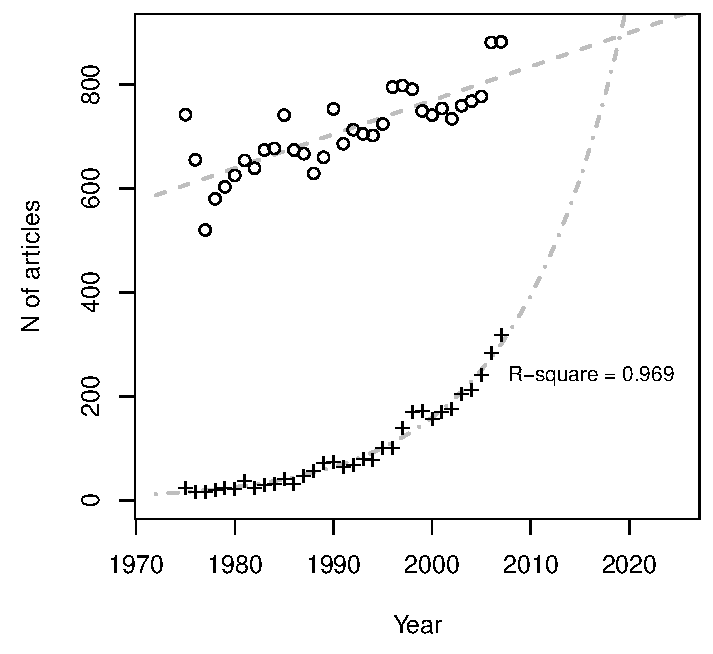
\includegraphics[width=.7\textwidth]{Fig_figure_from_Kliegl.pdf}
\caption{Comparison of publication growth rates\index{publication growth rates} in the field of psychology for national ($\mathtt \circ$) vs international (\texttt{+}) teams (this indicates that by 2020 there will be more trans-border author teams than national teams). This figure has been reproduced by using the script and data kindly contributed by \citet{Kliegl2011Scientometrics}. In comparison with Fig.\@~\ref{Fig:map_of_science}, one does not need to obtain copyright permission to generate new original visualizations and insights based on these data (hence our scientific creativity was not \emph{`locked'}).} \label{Fig:figure_from_Kliegl}
\end{center}
\end{figure*}

This document was, for example, produced using the \textsf{ScribTex}\footnote{\url{http://www.scribtex.com}}\index{ScribTex@\textsf{ScribTex}} collaborative editor. We started with a local copy. Once the book had reached 60\% of the final content, we placed it on-line and then continued writing into the live version only. \textsf{ScribTex} contains a full \textsf{TeXLive} installation customized to generate PDFs even if some artwork files are missing. Other alternatives for collaborative writing of {\LaTeX} documents are \textsf{LaTeXLab} and/or \textsf{Subversion}\index{subversion@\textsf{subversion}}. Once we finished writing the book jointly, we placed a copy on \textsf{A.nnotate.com}\index{collaboration!annotation} to get feedback from various colleagues (read-only access). We then moved on to prepare the Camera Ready Copy of the book.\par

In fact, you can easily install \textsf{MediaWiki} on a server, then add some plugins that allow the export of wiki text to {\LaTeX} or Open Office formats. There are now also efficient solutions that allow integration of programming (or any type of data processing) and document writing. For example, a package called \textsf{S--weave}\footnote{\url{http://www.stat.uni-muenchen.de/~leisch/Sweave/}}\index{S--weave} allows integration or \textsf{R} and {\LaTeX} code. That way statistical analysis and production of plots and tables can be automated, so that with any new iteration the authors only need to re-run the script and it will update the content using the new data. This means that the complete research article can be put into a single code (ASCII file) and co-authors can collaborate on different aspects (statistical computing, line editing, graphics and visualization) at the same time. Consider for example an article on the internationalization of research by \citet{Kliegl2011Scientometrics}. You can easily obtain the input data and \textsf{R} code used to generate all plots from the author's homepage and reproduce and/or extend the analysis (Fig.\@~\ref{Fig:figure_from_Kliegl}). \par

The idea of opening up both your data and the code you develop to process the data is very much in line with what Prof.\@ Pebesma\index{Pebesma} calls \emph{``the six pillars of open research''}\footnote{Edzer Pebesma's Inaugural lecture, University of M\"{u}nster, June 25, 2010. The complete talk is available at \url{http://www.opengeostatistics.org}.}. These are:

\begin{enumerate}
  \item \emph{open data, in real-time} (i.e.\@ data on a server)
  \item \emph{open source software}
  \item \emph{open, reproducable procedures}
  \item \emph{open, web-based methods for data and processing models} (interoperability)
  \item \emph{open and explicitly quantified significance and accuracy levels of research findings}
  \item \emph{managed, open user and developer communities}.
\end{enumerate}

This is probably too much to expect from every research group, but these principles are well worth considering.\par

Collaborative editing is becoming a standard way of producing articles, even when the co-authors are located along the same corridor. Papers produced by adopting such a process should be better because of the advantages listed above. Nevertheless, before a group jumps into collaborative writing via a web browser or by using \textsf{subversion} or \textsf{Git}, it's probably a good idea to first agree on the issues discussed from page~\pageref{sec:one_page_concept} onwards.\par


\section{Free and Open Source Software}\index{Open Source Software}

\begin{quote}
    \emph{``To build a better world we need to replace the patchwork of lucky breaks and arbitrary advantages that today determine success --- the fortunate birth dates and the happy accidents of history --- with a society that provides opportunities for all.''}\footnote{Malcom Gladwell in \emph{``Outliers''}.}
\end{quote}

In 1983, Richard Stallman\index{Stallman}, frustrated by some poorly implemented printer drivers, launched the free software movement and two years later published the GNU Manifesto. The GNU General Public License\footnote{\url{http://www.gnu.org/licenses/gpl.html}}\index{GNU General Public License} was published in 1989 and the first functional Linux operating system was released in the early 1990s. From then on, we've seen numerous examples of Free and Open Source\index{Free and Open Source Software} (FOSS\footnote{FOSS is a widely accepted abbreviation for software either registered under GPL or liberally licensed to grant the right of users to use, study, change, and improve its design by making its source code freely available.}) software projects that have been developed in parallel with commercial versions. At the beginning of the 21st century, we can say that FOSS has a solution for most of the commercial software applications needed to run a professional business (including scientific production and publishing). Here are some examples of popular FOSS used by academia (the numbers in brackets indicate the number of unique visitors according to \textsf{Google Ad planner}\index{Google Ad planner@\textsf{Google Ad planner}}):

\begin{itemize}\index{Open Source Software!list}
  \item \emph{Web-browsing}: \textsf{Mozilla Firefox} (210M)
  \item \emph{Office work}: \textsf{OpenOffice} (7.3M)
  \item \emph{Operating System}: \textsf{Ubuntu} (4.3M)
  \item \emph{Database management}: \textsf{MySQL} (3.8M)
  \item \emph{General-purpose web programming}: \textsf{PHP} (6.2M)
  \item \emph{Web publishing and Content Management System}: \textsf{Drupal} (3.1M)\index{Content Management System}
  \item \emph{General-purpose high-level programming}: \textsf{Python} (1M)
  \item \emph{Statistical programming}: \textsf{R} (320K)
  \item \emph{Scientific writing and document generation}: \textsf{{\LaTeX}} (120K)
  \item \emph{Collaborative editing / version control system}: \textsf{Subversion} (110K)
\end{itemize}

\begin{figure*}[!htb]
\begin{center}
  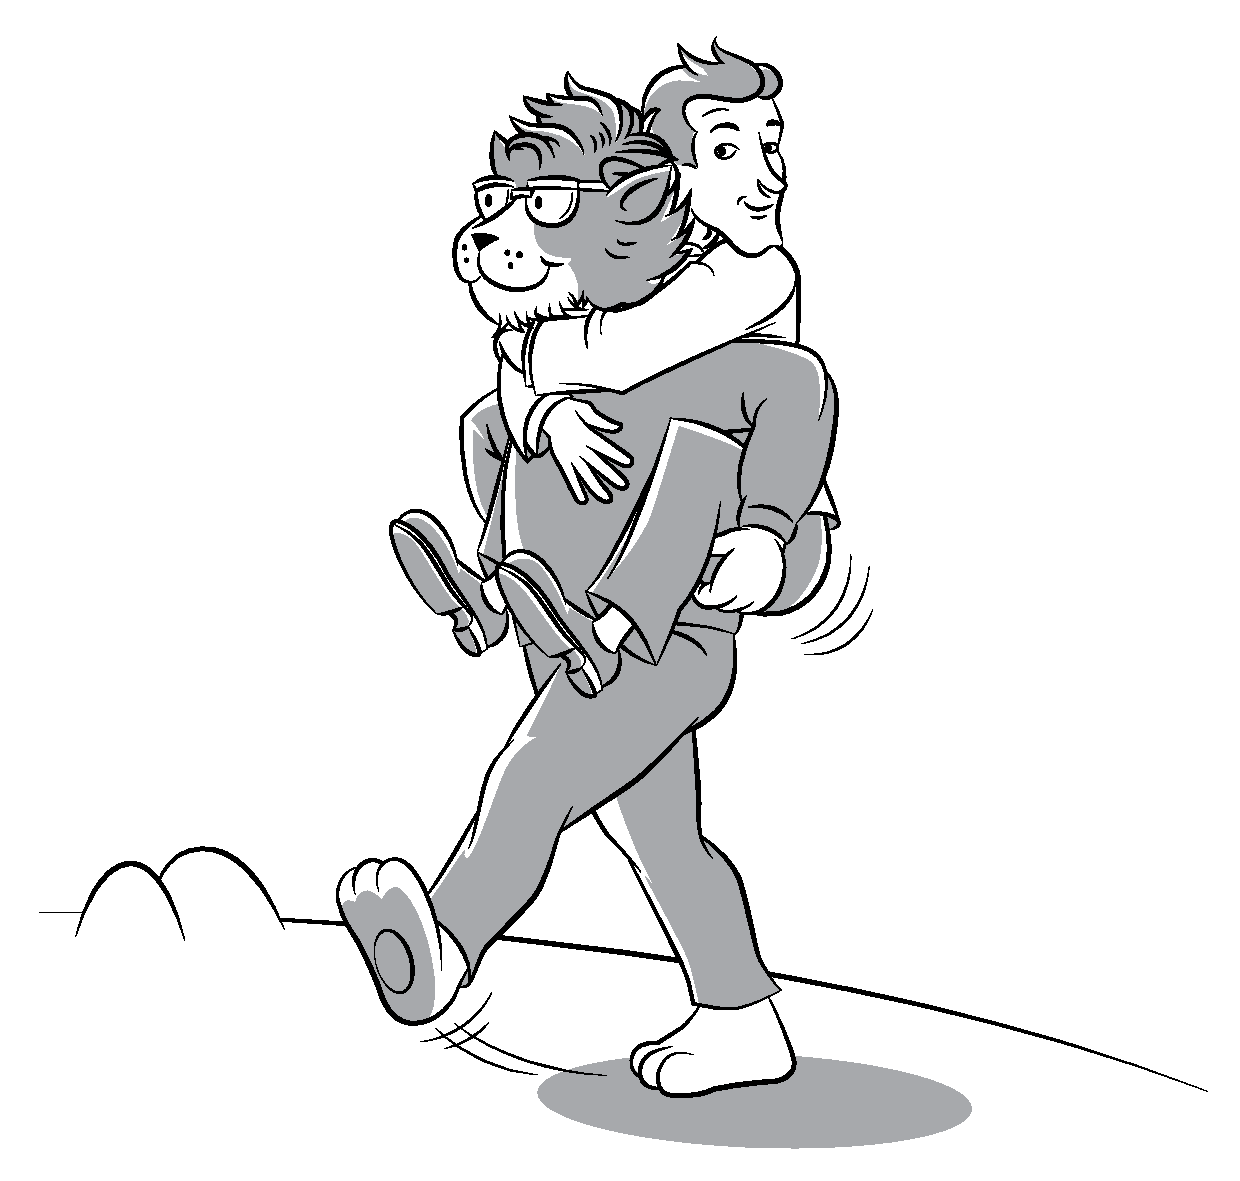
\includegraphics[width=.6\textwidth]{Fig_with_a_bit_of_help_from_TeX.pdf}
%\caption{With a bit help of \TeX.}
\label{Fig_with_a_bit_of_help_from_TeX}
\end{center}
\end{figure*}

Although they are available free of charge, all of these software packages are highly professional. They are maintained by active communities of developers, who are often top programmers/scientists and have an extensive publication history behind them.\par

For an academic or anyone working for a government agency or NGO (i.e.\@ a public servant) it makes absolute sense to use and promote FOSS. However, experience teaches us that few people have adopted FOSS as the main software suite for their work. Why? There are several reasons. First, commercial software companies market their products more aggressively. They often spend a great deal of money on advertising in newspapers, multimedia and on the internet, but also on visits and presentations to potential clients\footnote{Google's staff, for example, spend 70\% of time on search and advertising.}. FOSS groups, on the other hand, do not spend any money on promoting new releases.\par

Second, software first became a commercial business in the 1970s and 80s and many big software companies are still dominant simply because people have got used to their software and most of their documents and files are still in their formats. Even though there is now a solution that could save companies and institutions a great deal of money\footnote{E.g.\@ Microsoft Office Professional costs about 500~US\$ per licence; Windows~7 professional costs about 200~US\$.}, many are slow to switch to FOSS, perhaps due to the high costs of training and data migration.\par

Third, FOSS requires additional skills to read the code. FOSS is, in fact, completely based on the ability of people to read the program code, i.e.\@ understand the programming languages behind it, and then adjust and/or improve it. Human nature is such that, as with any complex system, when people cannot understand the \emph{magic} behind the system --- it frightens them. \par

\begin{figure*}[!htb]
\begin{center}
  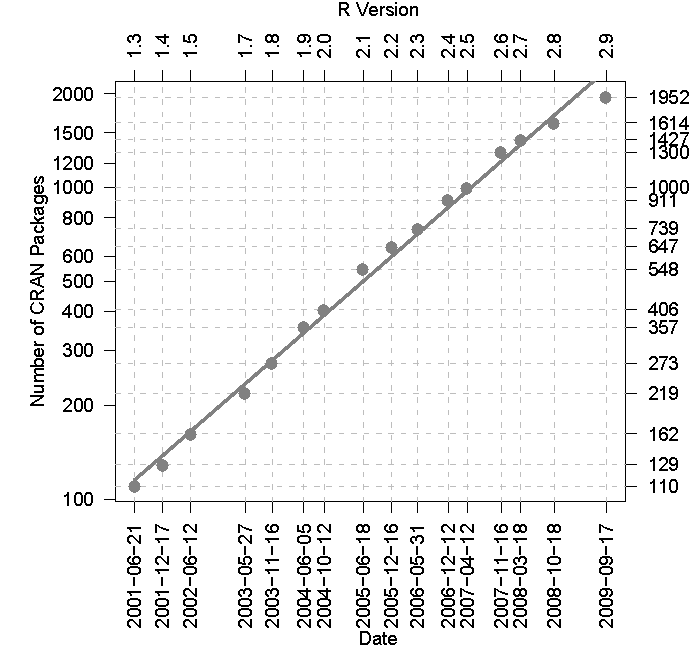
\includegraphics[width=.7\textwidth]{Fig_plot_RJournal_2009_2_Fox.png}
\caption{An example of a successful academic FOSS project is the \textsf{R} software for statistical computing \citep{chambers2008software,Kabacoff2011}. A growth in the number of contributed packages (submitted on the Comprehensive \index{software!\textsf{R}}\index{Open Source Software!\textsf{R}}\textsf{R} Archive Network) has been exponential, although the core group of developers consists of only a dozen researchers/enthusiasts. Plot taken from \citet[Fig.3]{Fox2009RJournal}.} \label{Fig_plot_RJournal_2009_2_Fox}
\end{center}
\end{figure*}

Most people still use commercial software from Microsoft, IBM, Apple or Oracle to run their projects. Even NGOs and academic institutions mainly use commercial software. The situation is, however, changing. Today, even commercial companies are discovering the advantages of using open source software. IBM, for example, is increasingly shifting its focus to using open source software, mainly Linux for web applications. Oracle distributes and maintains the \textsf{OpenOffice} suite. Sun maintains Java development software. So while commercial (closed code) software is still the mainstream, there is an unstopable trend toward opening up the code. To learn more about FOSS visit \textsc{Wikipedia}'s free software portal\footnote{\url{http://en.wikipedia.org/wiki/Portal:Free_software}}.\par

Ironically, support received from developers of FOSS is often of higher quality then that received from many commercial software companies. As Rolf Turner puts it:

\begin{quote}
    \emph{``In the middle of a Saturday morning (in my Time Zone!) I send out a plea for help, and in just over 20 minutes my problem is solved! I don't think you get service like that anywhere else. This R-help list is BLOODY AMAZING!''}
\end{quote}

This book was largely produced using FOSS. The text was typeset in {\LaTeX}, several graphs were produced using \textsf{R} and Open Office. Although {\LaTeX} might seem difficult for those who are not used to looking at the code\footnote{There are also user-friendly WYSIWYG editors for {\LaTeX} such as \textsf{Scientific WorkPlace}.}, you should at least try it. Maybe the professional layout of this book will convince you to consider switching to FOSS. \par

We are not saying that switching to FOSS is a MUST for everyone all the time\footnote{In this book we've also used commercial software. For example, most of the artwork was produced using Microsoft \textsf{Visio} and \textsf{Corel Draw}.}, but FOSS does need to be encouraged, especially if you work for government-funded projects and/or in education.\par


\section{The abstract}\index{abstract}

The last stage of writing is usually to generate an abstract and choose the official title for your paper. Titles and abstracts are important because these are the parts of your article that will be read an order of magnitude more often than the article itself. So it's a good idea to spend more time on producing them. Writing abstracts requires a lot of skill, because they must be compact, complete and full of useful information. Fig.\@~\ref{Fig:cham_abstracts} shows Jorge Cham's\index{Cham} view on the way people write abstracts.\par

\begin{figure*}[!htb]
\begin{center}
  \includegraphics[width=.9\textwidth]{phd011409s.jpg}\\
\caption{Writing abstracts by Jorge Cham, author and creator of the PhD Comics magazine. \emph{``Piled Higher and Deeper''} by Jorge Cham \url{www.phdcomics.com}.} \label{Fig:cham_abstracts}
\end{center}
\end{figure*}


\begin{svgraybox}
There is about a 10 times higher probability that somebody will read the title and abstract of your paper than the paper itself. You should therefore spend about 10 times as much effort on writing (and rewriting) them.
\end{svgraybox}

In fact, it's a good idea to write abstracts based on a template (though not the fill-in form Cham jokingly presents). For example, you can try the six-sentence template that was used to produce the paper in the appendix:

\begin{enumerate}
  \item \emph{What is this paper about, what is the topic and/or key objective?}
  \item \emph{What was the experimental design?}
  \item \emph{Which methods and materials were used to analyze the data / produce the results?}
  \item \emph{What do the results show (what was discovered)?}
  \item \emph{What are the main conclusions?}
  \item \emph{What are the (broader) implications of this work?}
\end{enumerate}

Abstracts are usually written in the passive form and the past tense (they describe what was done and why). In fact, the best abstract could well be written by a close colleague who is familiar with the topic and has read and understood the paper (almost like a review).\par

\begin{figure*}[!htb]
\begin{center}
  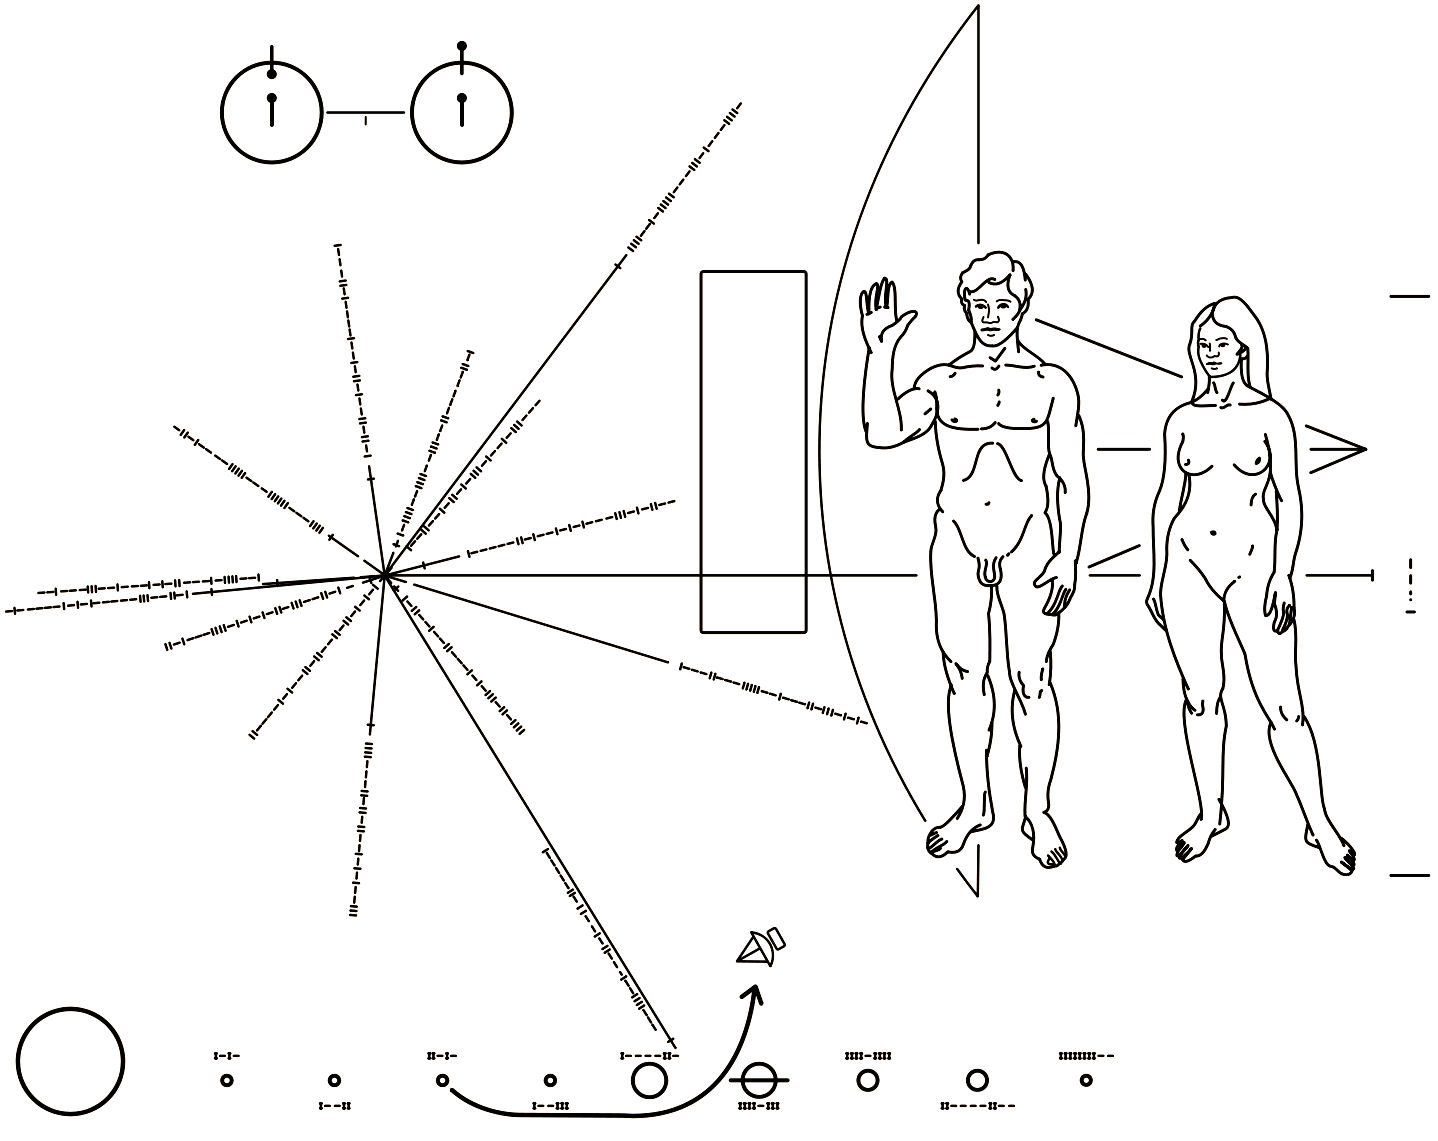
\includegraphics[width=\textwidth]{Pioneer_plaque.jpg}
\caption{NASA image of Pioneer 10's famed Pioneer plaque. A summary of our solar system, and of the creatures who made the Pioneer\index{Pioneer plaque}. Although it looks like abstract art, this drawing is actually packed with information.} \label{Fig:Pioneer_plaque}
\end{center}
\end{figure*}

Abstracts should be packed with technical information. See for example \emph{``Life on planet Earth: a one-page summary''}\index{one page summary} written by Nick Trefethen\footnote{\url{http://people.maths.ox.ac.uk/trefethen/}} --- this is not really an abstract, but it illustrates how to write compactly. Fig.\@~\ref{Fig:Pioneer_plaque} shows another example of an impressively compact abstract --- the Pioneer plaque showing the symbolic representation of our solar system using \emph{`universal'} measures. Too bad that researchers are not allowed to use such graphical symbols to produce summaries of their work, too. \par

Another thing to consider when writing abstracts is that abstracts should \emph{`sell'} an idea. Most readers use the title and abstract to decide whether to read your paper. They are a bit like an elevator pitch. \emph{``Elevator pitch''} reflects the idea that it should be possible to deliver the essence of an idea/proposal in the time span of an elevator ride (approximately thirty seconds to two minutes). With an abstract you get a similar opportunity: convince someone that your results are interesting using just a few lines of text.\par

\begin{svgraybox}
An abstract is a miniature version of the article. It should try to answer (at least) the following six questions: (1) What is this paper about? (2) Which experimental design was used? (3) Which methods and materials were used? (4) What do the results show? (5) What are the main conclusions? (6) What are the implications of this work? Abstracts should be packed with relevant information. Sentences should be short and (mainly) in the past tense.
\end{svgraybox}

Both abstract and title need to be accurate representations of the content of the article. If a reviewer is not able to find the information promised in the title or abstract, then their confidence will be seriously reduced. In fact, it's the ethical responsibility of authors to accurately reflect their work in the abstract and title.\par


\section{The title}\index{titles}

\begin{quote}
    \emph{``The way to create art is to burn and destroy ordinary concepts and to substitute them with new truths that run down from the top of the head and out from the heart.''}\footnote{Charles Bukowski in \emph{``Sifting Through the Madness for the Word, the Line, the Way''} (2003).}
\end{quote}

The basic function of the title of a research paper is to accurately reflect its content and main discoveries. A title should answer the simple question \emph{``what is this work about?''} (using the least possible number of words). Here's Jorge Cham's view of the way PhD students tend to generate titles for their theses\footnote{``Piled Higher and Deeper'' by Jorge Cham \url{www.phdcomics.com}.}\index{Cham}:\par

\medskip
\begin{center}
  \includegraphics[width=\textwidth]{phd053106s.jpg}
\end{center}

Indeed, many titles of research articles are a combination of catch phrases, boring expressions and terms that only a limited group of people really understand. Can we do better? Absolutely.\par

The best way to get inspired about generating titles is to look at inspiring examples. We will now list some titles that might give you an idea how to brainstorm a winning title. Let's start with a classic:

\begin{quote}
    \emph{``An index to quantify an individual's scientific research output''}\footnote{by J.E. Hirsch; published in 2005 in the PNAS journal.}
\end{quote}

This is the paper we refer to in the first part of this book, which introduces the $h$-index (named after the author). What it nicely shows is that the author takes a balanced view of its discovery: he mentions \emph{``an''} index, and then specifies what it's for. The author could have suggested the name for this index to avoid ambiguity, but we all now know that this is the key source that describes the previously mentioned $h$-index (see page~\pageref{Fig:citations_h_index}). We advise you to read this article not only because of its title, but also because it's a good example of a well-written compact paper that made history. \par

Here's another example of a good title:

\begin{quote}
    \emph{``Testing Hubbert''}\footnote{by Adam R. Brandt; published in 2006 in the journal Energy and Policy.}
\end{quote}

This paper shows extensive results from testing the Hubbert oil-reserves calculation model (a bell-shaped curve in which the area under the curve is equal to estimates of the total amount of oil available) using global oil production data. It won the Best Student Paper Award Competition at the 26th North American Conference of the International Association for Energy Economics, not only because of its intriguing title, but also because it is high-quality scientific work. What's so good about it? Several things:

\begin{enumerate}
  \item It's intriguing --- it promises an interesting read.
  \item It's short and catchy.
  \item In fact, it's so short and catchy that people notice it. It's as if the author has invented a new style for  making titles. Originality is always inspiring.
\end{enumerate}

The author could have easily used a longer, more explanatory title such as:

\begin{quote}
    \emph{``Statistical evaluation of the Hubbert model for prediction of the total remaining amount of oil in the world''}
\end{quote}

But the author doesn't try to explain what \emph{``Hubbert''} means. Everyone who reads that journal is already familiar with Hubbert's curve, so there's no need to explain it. Even someone who's not an expert in the field could figure out that it is about Hubbert's curve by quickly Googling the term. It's also clear that word \emph{``testing''} refers to statistically matching actual measurements with the model. By removing redundancy the author creates something that is catchy, while being completely accurate about the topic of the paper. \par

Trimmed titles are not always better. For example, \citet{BeelGipp2009} discovered that Google Scholar's ranking algorithm puts high weighting on words in the title. A longer title that includes all keywords might improve the chances that people will be able to find your work, so consider using the main keywords; then remove all redundancy, personal (and/or professional) bias, and ambiguous buzzwords from the title.\par

\begin{svgraybox}
Probably the best way to generate a title of a research article is to find a balance between using the key terms / discoveries and length. Titles can be also improved by removing redundancy and bias --- emotionally loaded words, overselling statements and ambiguous buzzwords.
\end{svgraybox}

Here's a longer example:

\begin{quote}
    \emph{``Wealth and happiness across the world: material prosperity predicts life evaluation, whereas psychosocial prosperity predicts positive feeling''}\footnote{by Diener \emph{et al.}; published in 2010 in the Journal of Personality and Social Psychology.}
\end{quote}

This paper explores the connection between happiness, income, and psychological needs. Although the title seems to be rather long, it has an original element: it puts the most important conclusion in the subtitle and hence efficiently conveys the main message. We almost don't need to read the abstract! It's an original research paper that reports novel results, so it helps to see these results in the title. \par

\bigskip
\begin{fminipage}{.9\textwidth}{\footnotesize{\textsf{\textbf{Do buzzwords work?}}\index{buzzwords} --- Buzzwords are new fashionable terms that are used in the media. Buzzwords typically have a negative connotation among scientists because they indicate that some originally technical term is now used \emph{``pretentiously and inappropriately by individuals with little understanding of its actual meaning.''} Some typical examples are: cyberspace, sustainability, nanotechnology, cloud computing, and E-learning. Intuitively, a buzzword can increase the visibility of your paper --- buzzwords are catchy. But you should also be critical. First, you need to think of the buzzword as a dynamic thing: what will happen to it in five to ten years' time? Will it still be as popular? Some quite recent buzzwords now seem ridiculous.}}
\end{fminipage}
\bigskip

Here's a somewhat different example, this time the title of a book:

\begin{quote}
    \emph{``Does God Play Dice? The New Mathematics of Chaos''}\footnote{A book by Stewart, I.\@ published by Blackwell in 1989.}
\end{quote}

In this example the author uses a famous quote by Albert Einstein to intrigue his audience. A title without this quote would have been as accurate but, because it's a book on popular science, an intriguing title will attract a wider audience. In research articles, it's often also effective to place a big research question directly in the title. Just make sure you provide an unambiguous answer to that question.\par

Another example, this time from The Economist:

\begin{quote}
    \emph{``Organising the web: The science of science''}\footnote{\url{http://www.economist.com/node/18618025}}
\end{quote}

This is an article about developments in the field of web-crawling and automated categorization. Probably too general a title, because science and scientific systems cannot be simplified to web-crawling. If you look at this article you will notice that it only presents some initial results from a small group at Princeton University. This tells us more about the authors\footnote{Interestingly enough, The Economists does not publish the names of authors with their articles (hopefully a model no scientific journal will follow), so we don't even know who stands behind this article.} of the article than about the topic. \par

Based on these examples, we can roughly classify journal article titles into six groups:

\begin{itemize}
  \item \emph{Topic in the title} --- The title here is basically the field of study. The advantage of such a title is that it can be relatively short; the disadvantage is that the title is not dynamic and is probably more general than the content of the paper. \smallskip
  \item \emph{Topic : subtitle} --- A somewhat better version of the topic-type title is a title with a sub-title that refers to the main discovery/key claim. \smallskip
  \item \emph{Claim in the title} --- The title is the key claim. See the example by Diener \emph{et al.} on the previous page. \smallskip
  \item \emph{Research question in the title} --- A title can also be formulated as the key research question, finishing with a question mark. This type of title is somewhat unconventional --- not acceptable in all fields, hence risky. \smallskip
  \item \emph{Sub-field in the title or subtitle} --- An ambitious way to generate titles is to literally invent new sub-fields. This might not be well received in every discipline, but it is a good idea to attach a subtitle (to an ambitious title) specifying the focus of your study. \smallskip
  \item \emph{Free title} --- A title that does not belong to any of the above categories can be classified as an \emph{``free title''}. Some researcher like to demonstrate that complex thinking and a sense of humor go well together. Is it appropriate to demonstrate a sense of humor in the title of a research article? Usually not, but it's a challenge you could consider. Journals typically do not welcome controversial titles, but if you have really good results you might just get away with it.
\end{itemize}

Nancy Ackles\footnote{\url{http://depts.washington.edu/eslinfo/Lab/titles.html}} suggests three general strategies for naming a paper:

\begin{enumerate}
\renewcommand{\labelenumi}{\Roman{enumi}}
  \item The title should be a noun phrase, not a sentence or a noun clause.
  \item The title should indicate the topic of the paper.
  \item The title should be unambiguous and use only standard English word forms.
\end{enumerate}

There is also the issue of redundancy, which is a common mistake many authors make. Most editors agree that you should avoid using titles that contain expressions such as \emph{``Some new results''}, \emph{``A novel method for''}, \emph{``An investigation of''}, \emph{``Effects of''} etc. If you want to trim your title, this is where you should start. And always check the heading style in the journal you have targeted to make sure your heading matches that style.\index{redundant words}\par

It's the author's responsibility to use a title that closely reflects what is presented in the manuscript. You don't want to either undersell or oversell (too general topic in the title/too many buzzwords). If you oversell, someone might read your article and get disappointed. Unlike in show business\footnote{People in show business often say that there's NO such thing as bad publicity: all publicity is good.}, in science there \emph{is} such a thing as bad publicity. \par

\begin{svgraybox}
The title should exactly cover the content of the article and/or express its main claim. Nothing more, nothing less.
\end{svgraybox}\label{R:title}


\section{Final tips}

\begin{quote}
    \emph{``The only end of writing is to enable the readers better to enjoy life, or better to endure it.''}\footnote{Samuel Johnson in his review of Soame Jenyns' \emph{``Free Enquiry into the Nature of the Origin of Good and Evil''}.}
\end{quote}

The first draft of your article will probably just be \emph{``an incoherent stack of notes you've written to yourself''} \citep{Clark2003}. But this should not worry you because most high-quality papers go through ten or more editing iterations. In fact, for Zissinger, the essence of writing is rewriting\index{rewriting}. As \citet{Creedy2008research} also puts it: \emph{``Perhaps the most important rule of writing is that the first draft is not the final draft but is simply the start of a long process of revision.''} \par

Even if you are just putting the pieces together, you should check whether your first draft contains the following main elements (after Ed Hull):

\begin{itemize}
    \item \emph{The `big picture'} --- the background to your research and why it's important.
    \item \emph{The purpose statement} --- what you set out to show.
    \item \emph{How you went about answering the research question} --- what you did.
    \item \emph{The answer to the research question} --- what you concluded.
    \item \emph{The answer to the \emph{so what?} question} --- why should the reader care?
    \item \emph{The consequences for future research} --- which could change the original `big picture'.
\end{itemize}

For more detailed tips 'n tricks, see our \emph{``Rules of thumb for writing research articles''} in the appendix. If you follow these guidelines closely, you should be able to produce a first draft of your article, which you can then revise and polish to \emph{`perfection'}. \par

When you re-read your paper, you may still be unhappy with it. It might have many novel elements, but if you feel that something is missing --- excitement, enlightenment, sparkle$\ldots$  call it what you will, such papers will not make much of an impact in science. Go back to your title, introduction and discussion and see if you can strengthen the story you are telling in your article. The points that you are trying to make need to be clear and strong. You should not be afraid of contributing new thoughts. And don't forget that scientific writing is both a science and an art. As Samuel Johnson put it: \emph{``What is written without effort is generally read without pleasure.''}\par

If you find line editing difficult, you could consider getting professional help. There is a thriving article editing business \citep{Kaplan2010N}. There are now numerous professional companies\footnote{Some international scientific editing companies: the Nature Publishing Group Language Editing in London, MacMillan Scientific communications, Carter's Strategic Solutions, and American Journal Experts.}\index{scientific!editing companies} that charge a reasonable price (in the range 300--500~US\$ per article) for reading your paper and giving you comments and suggestions.\par

An experienced writer will usually take at least three to five iterations until he/she produces a version that is ready for submission. If you and your co-authors are not longer sure what to leave out and what to extend, this is a sign that you should now send the paper to the journal. Time is also a factor --- science rewards only those who publish first. It's not a good idea to keep going round in circles with your co-authors. Or as Blaise Pascal once said: \emph{``thinking too little about things or thinking too much both make us obstinate and fanatical.''}\par


%%%%%%%%%%%%%%%%%%%%%

\chapter{Submitting your article}\label{sec:submitting}


Prior to submitting your article, we strongly recommend seriously investigating the journal (looking at the editorial board, previous issues, list of authors and their academic level) in which you intend to publish your work. There are still many things that you need to consider to avoid your paper ending up in the editor's waste bin.\par

 \section{Find the right journal}\index{how to find a journal}

\begin{quote}
    \emph{``We are at a turning point in our history. Universal access is the goal. And the opportunity of leading a different life, based on this is$\ldots$ thrilling. It could be one of the things humankind would be most proud of.''}\footnote{Brewster Kahle cited by Lawrence Lessig in \emph{Free Culture}.}
\end{quote}

Once you have prepared a one-page concept paper, you should already have a good idea about where to publish your full manuscript. Your paper needs to closely match the scope and format of the journal; otherwise, even if it is a very promising paper, it may well be rejected (right message in the wrong place). If you have a list of possible journals, now is the time to think about which is the best candidate. The ultimate tip is: always go first for the highest quality journal that may be interested in your topic. If this journal rejects the paper, you can always turn to the second on your list. But be realistic. Do not send articles of limited interest to top journals, otherwise you will waste people's time (including your own). The key question should be: who do I want to read my paper and which journals are those people scanning?\par

\citet{Babor2008} suggest the following key steps when selecting a journal:

\begin{itemize}
  \item \emph{Decide first whether the article is suitable for an international audience, either in a generic, disciplinary or specialized journal}
  \item \emph{Explore the compatibility between your article and the journal's culture (read the journal's mission statement)}
  \item \emph{Make sure the journal is currently interested in the type of article you have written}
  \item \emph{Gauge your exposure by reviewing the journal's circulation and abstracting service}
  \item \emph{Consider, but don't get fooled by, impact factors}
  \item \emph{Take into account time to publication and other practical matters}.
\end{itemize}

\begin{figure*}[!hbt]
\begin{center}
 \resizebox{\textwidth}{!}{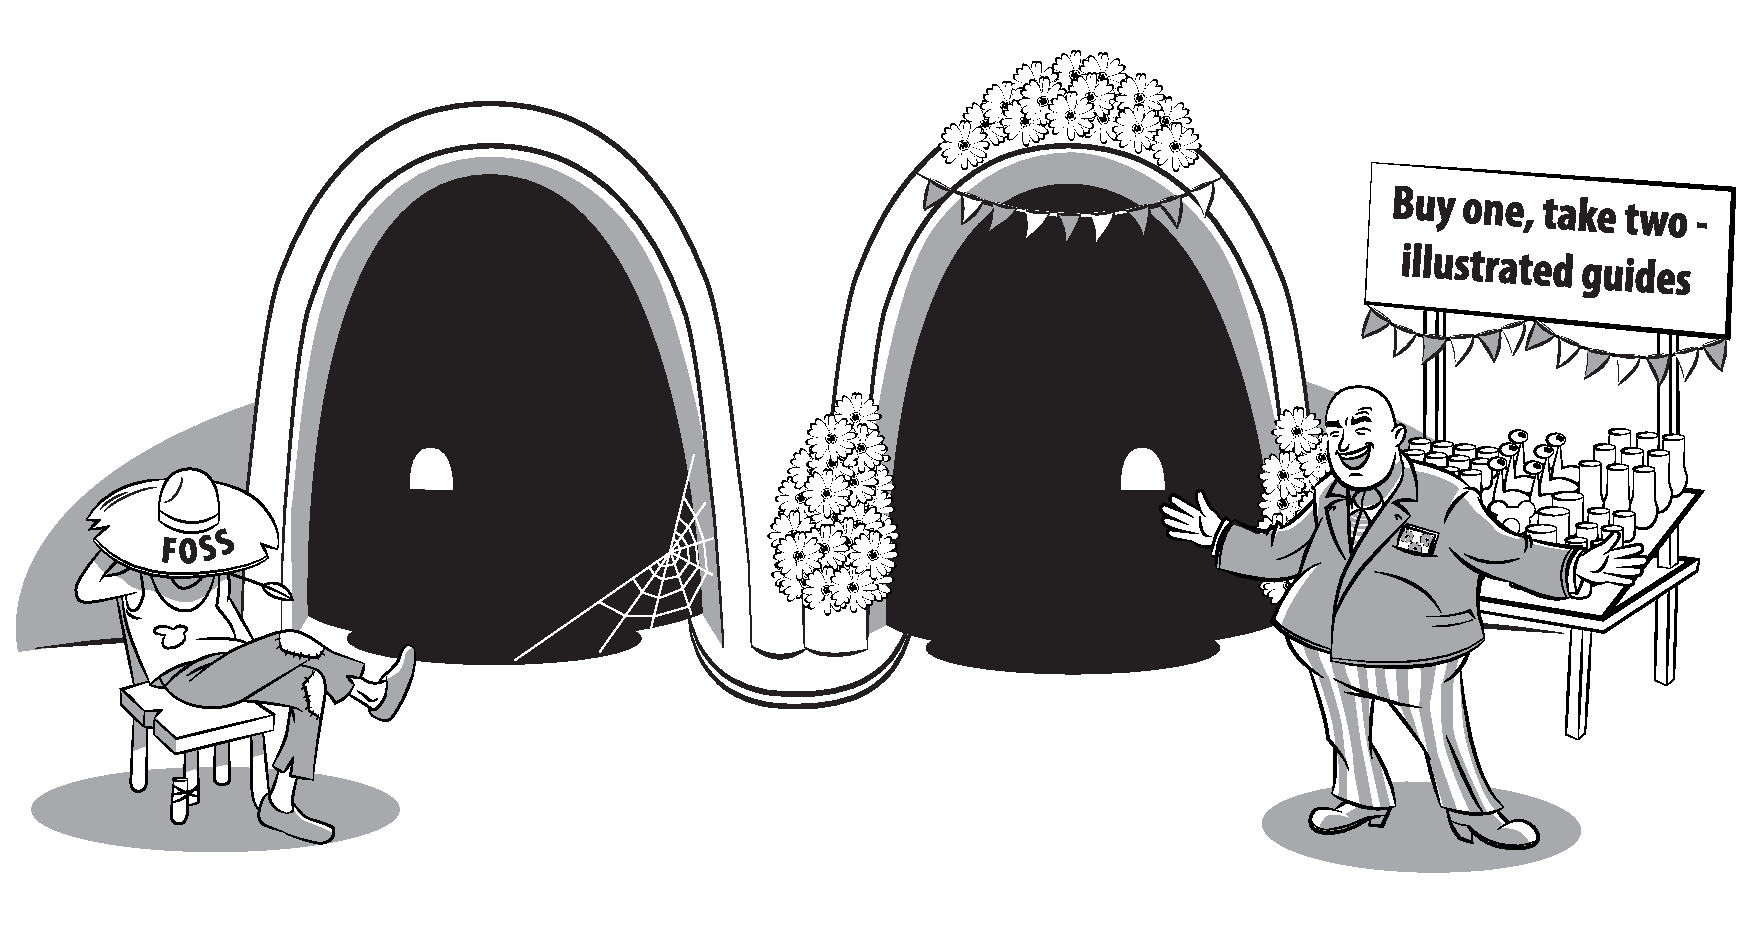
\includegraphics{Fig_tunnel.pdf}}
\end{center}
\end{figure*}

Scimago Labs provides a service called \emph{``SCImago Journal and Country rank''}\footnote{\url{http://www.scimagojr.com}}\index{SCImago}, which allows comparison of journals using a number of bibliometric indices --- citations per year, $h$-index, international collaboration, etc --- which makes it relatively easy to find out which journals in the field should be next on your list. \par

\begin{svgraybox}
Do not transfer your copyright to a commercial publisher too easily, because they will exploit it to eternity. There are plenty of reasonably priced Open Access publishers such as BioMed Central, PLoS, Copernicus, and MDPI, which are often indexed in SCI and have increasing visibility.
\end{svgraybox}\label{R:dontgiveC}

The following checklist can help you judge both the quality of a journal and the editorial process:

\begin{itemize}
 \item Check if the journal is indexed (by Thomson Reuters in the SCI or CC database). You can do this at any time from Thomson Reuters's Master journal list\footnote{\url{http://science.thomsonreuters.com/mjl/}}\index{Master journal list}\index{journal list} and/or via the SCImago website. If the journal is listed by Thomson Reuters, this will increase the chances that your article will be seriously considered. You can also check the impact of the journal or even the impact of the country\footnote{For example, the country with the highest number of citations per article in the last 10 years is Switzerland. It is also the country with the highest number of citations per researcher. See also \url{http://sciencegateway.org/rank/}.} where you intend to publish.
 \item Check if the article (or at least its abstract) will be available on-line in PDF format. This will increase the chances that it will be widely accessed.
 \item Check if your article will receive a unique identifier, such as a \textbf{Digital Object  Identifier}\footnote{See \url{http://doi.org} for more details.}\index{Digital Object Identifier}, which is something like an ISBN for books. This will make it easier to locate.
 \item Try to find out whether the journal provides English language and graphics editing. Journals usually do not do this, but you can often find out from colleagues. This will increase the chances that the article will be of high publication quality.
 \item Check if the journal has an on-line editorial system. This will help ensure that your article is not kept on hold for a long period of time.
 \item Try to find out if the journal offers a double-blind review and/or publishes review findings. This will help ensure that you receive an unbiased review.
 \item Check the Journal's (publisher's) copyright and self-archiving policy\footnote{\url{http://www.sherpa.ac.uk/romeo/}}\index{SHERPA} --- is the journal \emph{`green'}? Do they permit public access to author's pre-prints and/or post-prints?
\end{itemize}

Note that each journal has its own review system, preferred style and specific jargon. You should always make sure your paper meets the requirements of your target journal. \par

\begin{figure*}[!htb]
\begin{center}
  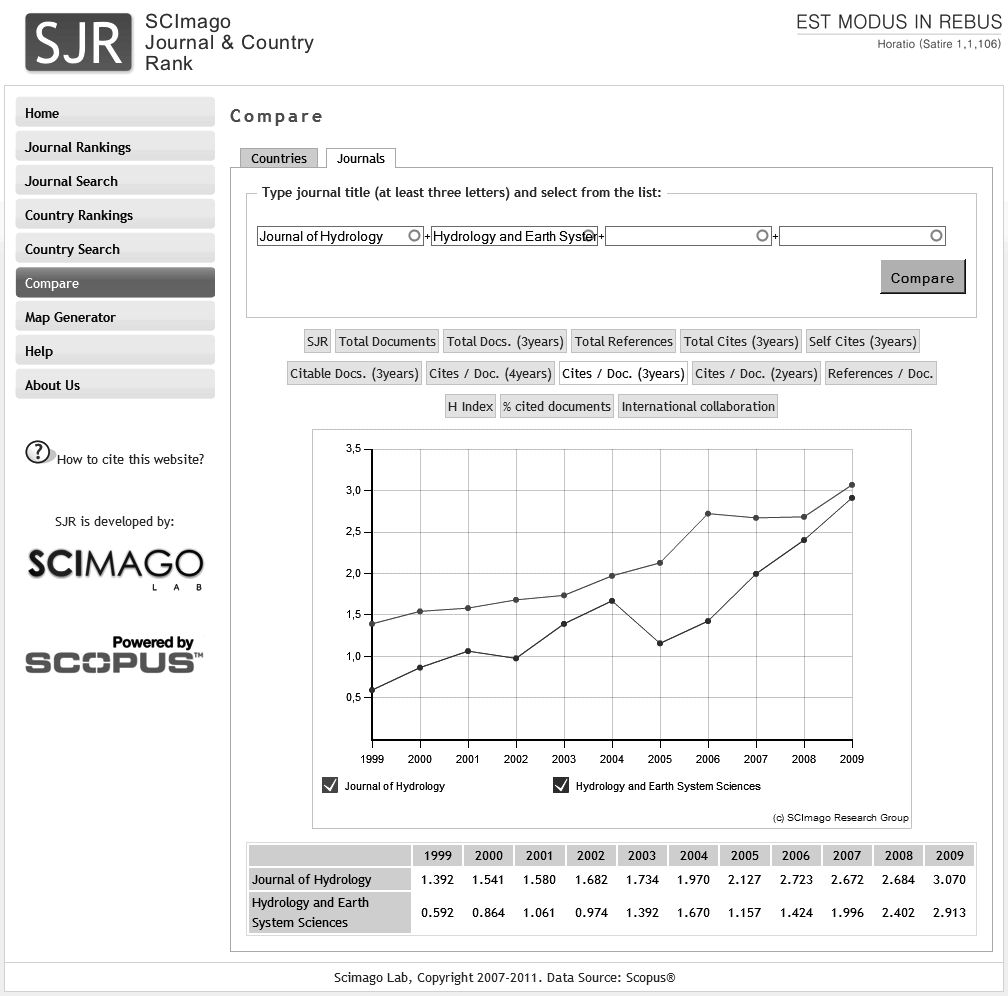
\includegraphics[width=\textwidth]{Fig_SCImago_screenshot.jpg}
\caption{Comparison of citations per year for articles published in one STM (Hydrology) and one OA (HESS) journal. Although many commercial publishers seem to offer more service and quality (at least that's what they advertising says), low-budget publishers can often do an equally good job.} \label{Fig:SCImago_screenshot}
\end{center}
\end{figure*}

\begin{sidewaysfigure}[!hbp]
\begin{center}
 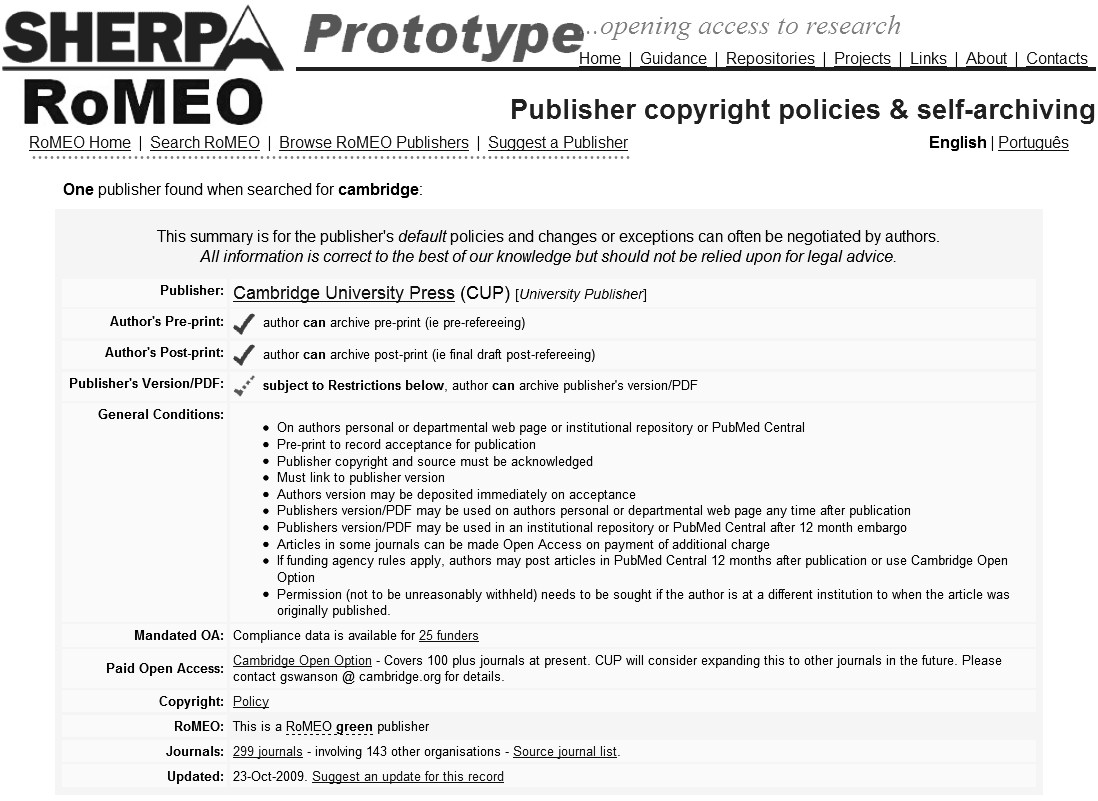
\includegraphics[width=.75\textwidth]{Fig_SHERPA_screen.jpg}
\caption{SHERPA (Securing a Hybrid Environment for Research Preservation and Access) provides an overview of publisher's policies. Worth checking before you select a journal.}
\label{Fig:SHERPA_screen}
\end{center}
\end{sidewaysfigure}



 \section{Do the work of the reviewers yourself}

\begin{quote}
    \emph{``Hard work is a prison sentence only if does not have meaning. Once it does, it becomes the kind of thing that makes you grab your wife around the waist and dance a jig.''}\footnote{Malcom Gladwell in \emph{``Outliers''}.}
\end{quote}

Another useful pre-submission tip is to try to do the work of the reviewers yourself (put yourself in reviewer's place) or give the paper to your colleagues and ask them to review it. Once you have created some psychological distance from the draft paper, you can read your work more critically. Reviewers usually complain about similar things --- either they are frustrated trying to understand your argument, they are not sufficiently convinced, or they are disappointed that you are not acknowledging their work.\par

The quality of a paper is determined by the quality of the \emph{spices} used to prepare it. For example, the quality of a new methodological paper can be determined by evaluating whether:

\begin{itemize}\renewcommand{\labelitemi}{$\checkmark$}
  \item the input data sets are of high quality (50\%\footnote{This number is an empirical estimate.})
  \item cross-evaluation of results is available (25\%)
  \item at least one alternative approach has been considered (10\%)
  \item a variety of validation indices have been used (10\%)
  \item a clear and honest discussion of limitations is provided (5\%).
\end{itemize}

\begin{figure}[!hbt]
 \begin{center}
  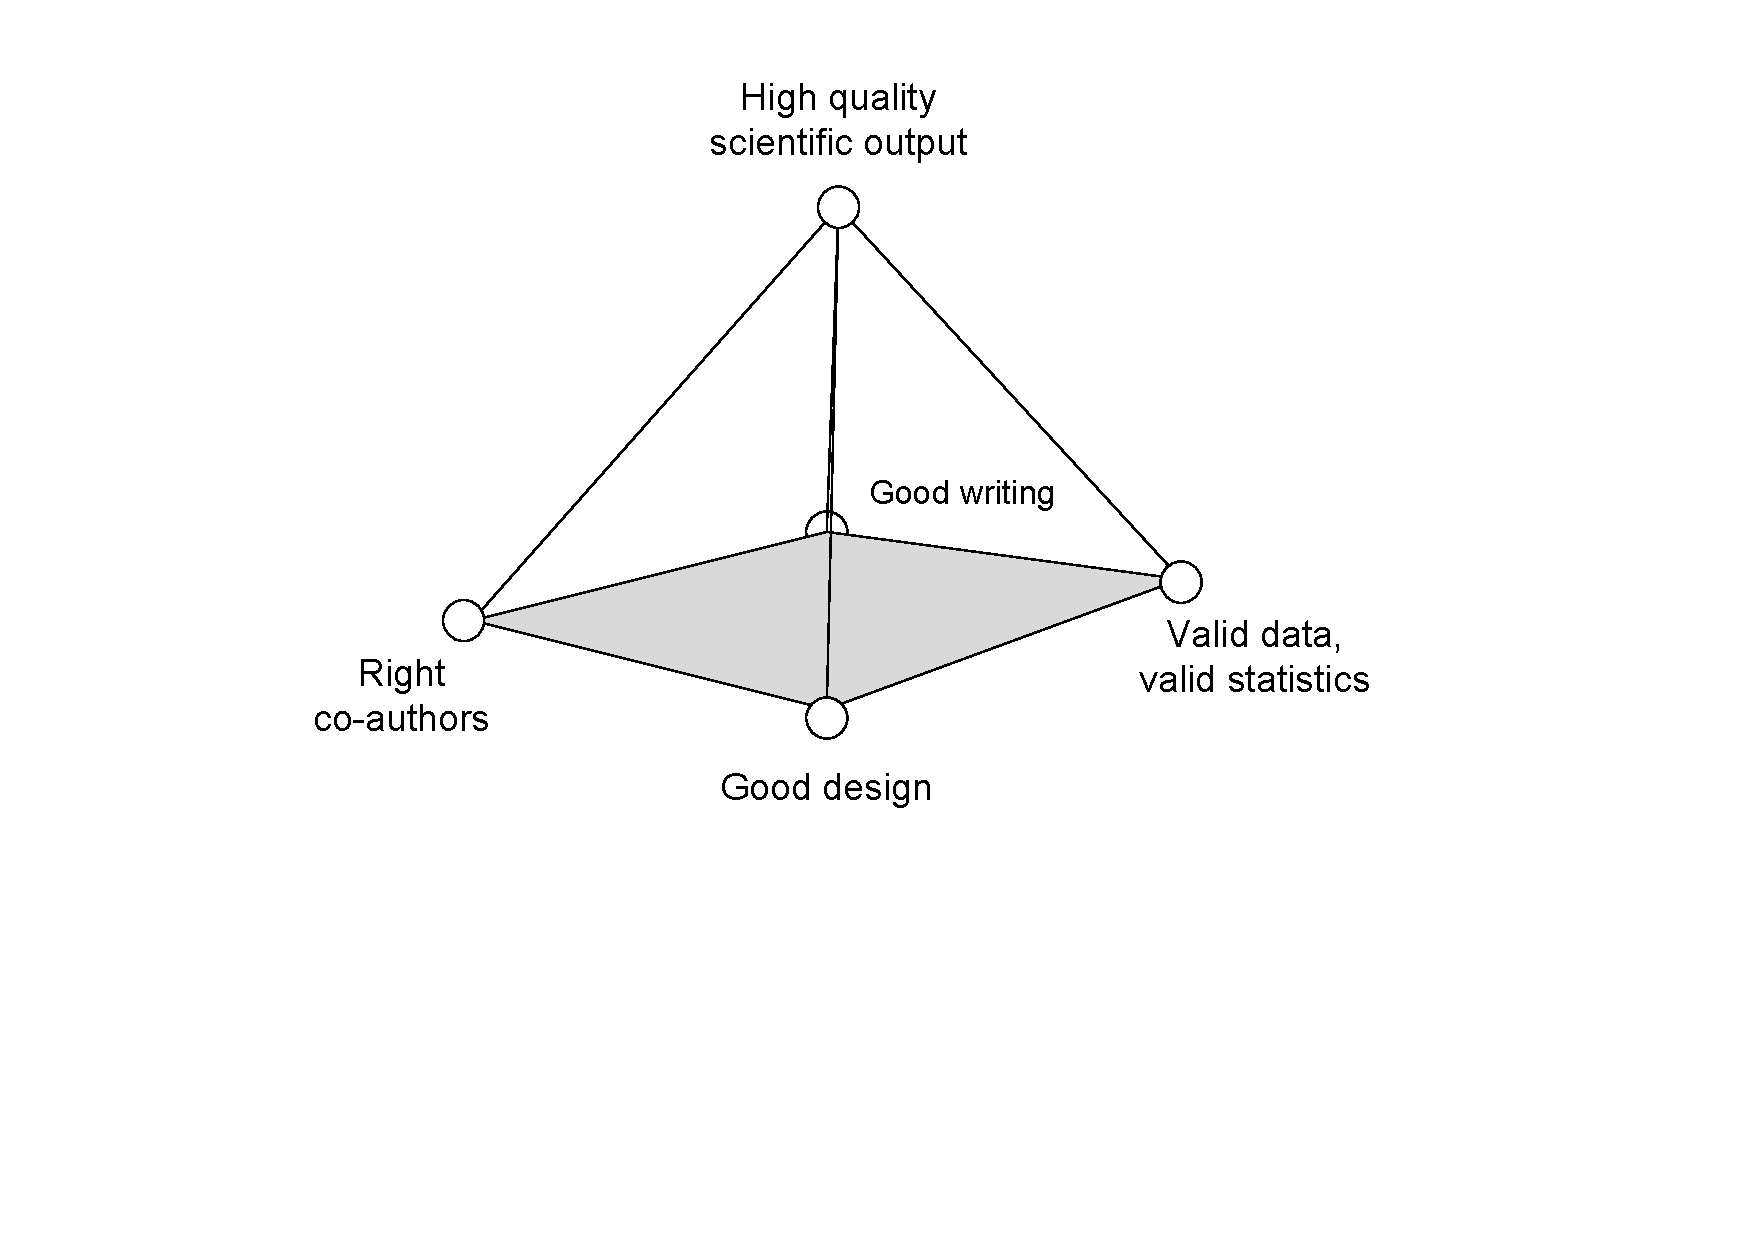
\includegraphics[width=.6\textwidth]{Fig_what_makes_good_paper.pdf}
 \caption{What makes a good paper? A combination of the right co-authors, good design, good data and good writing. See also the 10 rules for getting published on page~\pageref{sec:bourne_rules}.} \label{Fig:what_makes_good_paper}
 \end{center}
\end{figure}

This means that you can make a stronger argument if you:

\begin{description}
 \item[\emph{Consider alternative solutions}] \hfill \\
      Compare your method with alternative methods using rigorous criteria. Try to describe both the strong and weak aspects of your method in relation to alternative techniques. Recall the rules of science on page~\pageref{F:rules}: report your discoveries in an unbiased way; you should even try to challenge your own initial ideas. Big problems are seldom solved with a single study.\medskip
 \item[\emph{Test it under different conditions}] \hfill \\
      Evaluate the performance of your method using several case studies or experiments. How does the method work under different conditions, both global and local? How universal are your discoveries/conclusions?\medskip
 \item[\emph{Emphasize possible applications/implications}] \hfill \\
      If you give concrete guidance to readers on how to apply your methodology, this will certainly increase its impact.\medskip
 \item[\emph{Identify yourself with a broader research group}] \hfill \\
      Think of a research group as an international company in which you have shares. You need to support the work of your colleagues and find your identity (your \emph{niche}) in that company. This means that you need to be self-critical and acknowledge the fact that other colleagues might find better solutions. Modest opinions and statements are usually more accurate, but avoid too much hedging --- making weaker claims than those your paper justifies.
\end{description}

You may need to return to your data and even do some extra data collection. Although you might not feel like doing this, think about how you would react if you were to receive a negative review (rejection or serious revision needed). You might lose six or more months waiting for advice that you can anticipate now. \par

\begin{figure*}[htb]
\begin{center}
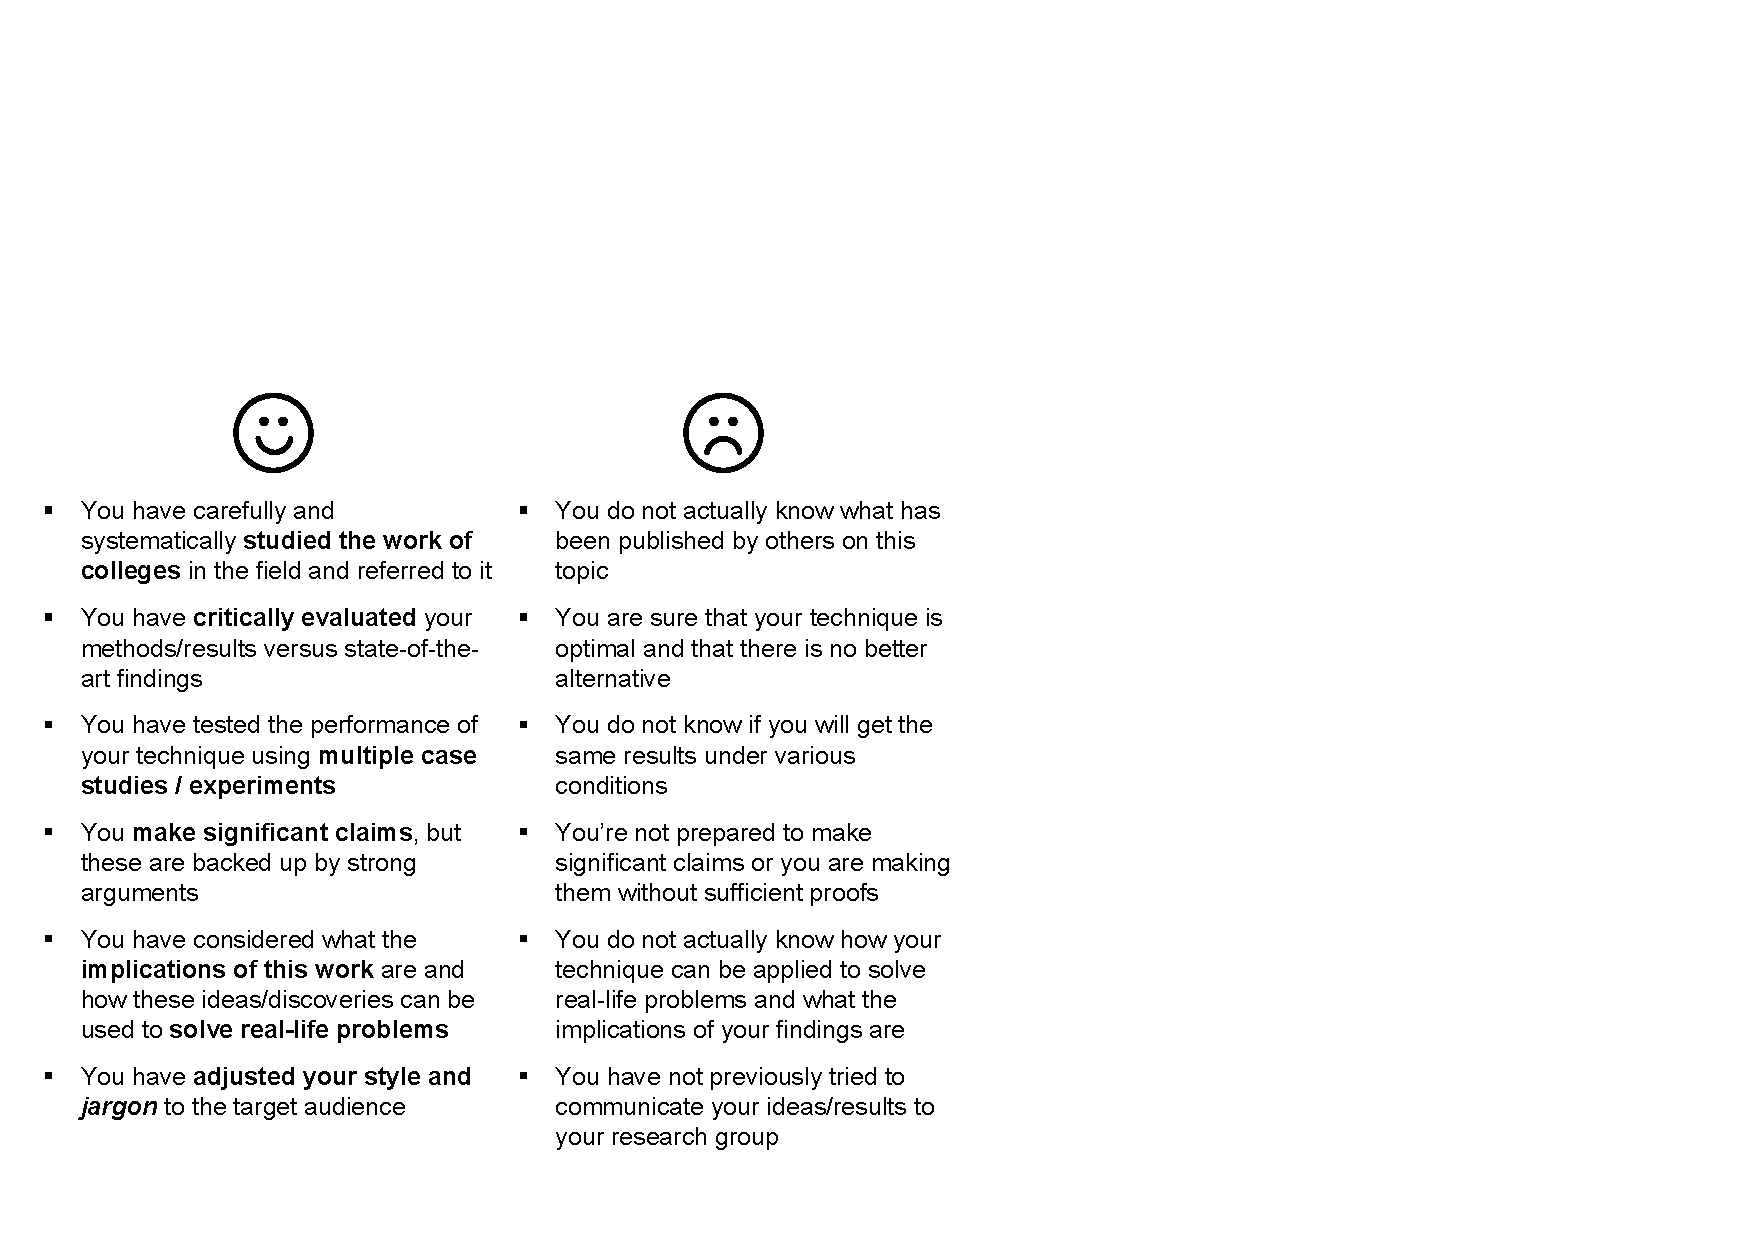
\includegraphics[width=\textwidth]{Fig_checklist.pdf}
\caption{Some Do's and Don'ts to consider before submitting your article.} \label{F:dos}
\end{center}
\end{figure*}

Make a multi-level description of your method/results --- go from the simplest to a more specific case and then on to a general case. A simple case study (that shows real numbers) will help readers understand the technique, while the multiple case studies will convince them that it works under a variety of conditions. The important thing is that readers can zoom in and out, depending on their interest.\par

Submitted research papers should not be draft documents but double and triple-checked manuscripts that are almost ready to go to print. You might think that some minor errors can be fixed later on, but for the reviewer just one fatal flaw (!) can excuse them from checking all of the subsequent details \citep{Smith1990TR}. \citet{Smith1990TR} is, in fact, a must-read for anyone who wants to understand how reviewers look at the papers.\par

\newpage

 \section{Make a full information package}

\begin{quote}
    \emph{``Some books seem to be written not to instruct, but rather to show that the author knows something.''}\footnote{Johann Wolfgang von Goethe 1749--1832 in \emph{``Maximen und Reflexionen II''}. This quote reflects the main difference between writing at university (for your professor) and for a real-world audience.}
\end{quote}

Reviewers get you published, but it's readers who get you cited. Prepare additional promotional material such as websites, posters, and brochures that can help people understand your work or convince them that the results are correct. In business, this is called \emph{post-production} and it's particularly well developed in show business --- Hollywood film companies, for example, spend enormous amounts of money promoting their new products.\par

Graphical elements can play a key role here because scientific information is often communicated more easily through figures. Sometimes it can help your paper if you include extra diagrams --- even sketches or photographs. Whatever helps you convey your message and draws attention to it is good. Your final product might include:

\begin{itemize}
 \item The core paper itself (typically about 15 pages of text).
 \item Technical notes or supplementary materials in which data collection, analysis and interpretation are evaluated in detail.
 \item A website where all supplementary materials/datasets can be found and accessed. A website is also useful for providing multimedia such as animations and videos. On the other hand, it is not a good idea to put your whole manuscript on the web before it has been indexed. \emph{`Gray'} publications are soon forgotten and there is a risk that someone else might take credit for your work.
 \item Promotional material such as brochures and posters, in which your key ideas/discoveries are presented in a popular way. An excellent tool is a \textsf{pubcast}\index{pubcast@\textsf{pubcast}} in which you talk to camera about your work and then link this clip to your paper\footnote{\url{http://www.scivee.tv/pubcasts}}.
\end{itemize}

According to Prof.\@ Edzer Pebesma (University of M\"{u}nster) scientists can increase their impact if they attach datasets and publish software that goes with their articles --- \emph{``People love to use software and/or datasets that come with a reference --- it makes them feel they do science. And to us, it's the number of citations that get us somewhere.''}\index{Pebesma}\par

There is now a general notion to publish the whole research so that anyone can reproduce and advance it. This is becoming increasingly important for scientific fields such as climate change and biodiversity assessment \citep{Kleiner2011}. \par

\newpage

\section{Pre-submission checklists}


\begin{quote}
\emph{``Progress in research is largely achieved by making a series of small steps, rather than taking giant leaps.''}\footnote{John Creedy in \emph{Research without tears}.}
\end{quote}

Even though your paper is starting to look complete and serious, you should not rush into submitting it to a journal. You can use the following checklist\footnote{Adapted from \citet{oConnor1975writing}.} to take one last look at the paper:

\begin{itemize}
  \item \emph{Do I still like the beginning?} Ideas evolve as you write --- sometimes it's best to write the Introduction last.
  \item \emph{Can I write more clearly, concisely and simply?} Avoid complex jargon, and replace pompous with plain language. Look at the text from the reader's point of view. Does it need to be so complex?
  \item \emph{Do I make sense?} Check for contradictions, ambiguity and poor logic.
  \item \emph{Do my numbers add up?} Check all figures and statistics carefully, or get them checked. If two numbers do not add up, reviewers start to rapidly lose confidence even if these are accidental typos.
  \item \emph{Do my sentences \emph{hang} together?} Write smooth, dynamic paragraphs (not all the same length).
  \item \emph{Do my verbs pull their weight?} Use strong verbs, keep them close to their subjects and make unnecessary passive formulations active.
  \item \emph{Do I need every modifier?} Delete non-essential adjectives and adverbs / keep them close to nouns and verbs.
  \item \emph{Have I got rhythm?} Listen to the sound of your writing. It should be easy to read out loud. If it is not --- re-organize, compress and improve connections in the text.
  \item \emph{Am I playing in tune?} Listen to the tone. Is it in harmony with your subject and your audience?
  \item \emph{Can I trim?} If in doubt, cut it out. Say things once, not twice or three times.
  \item \emph{Have I made my case?} Step back and assess the power of your arguments. Ask a colleague's opinion.
  \item \emph{How's my grammar and spelling?} Don't forget to run your spelling checker. But be skeptical about your software' grammar checker --- it's not foolproof.
\end{itemize}

Finally, you should check your contact details and affiliation. For affiliation, many recommend that you should avoid using a third level classification. For example, the most common affiliation is (1) university/institute + (2) research group. Adding more levels simply confuses people because most of the academic systems in the world are based on a \emph{legal entity} (company owner) + \emph{research group} (project / educational programme). Adding more than two classification levels can also lead to inaccuracies because most indexing services have only two levels in their database.\par


 \section{The review process and response to reviews}

\begin{quote}
  \emph{``When you meet someone better than yourself, turn your thoughts to becoming his equal. When you meet someone not as good as you are, look within and examine your own self.''}\footnote{Confucius in \emph{The Analects} (cca.\@ 475 BCE --- 221 BCE).}
\end{quote}

Before or during the review process, you should also consider some of the following tips, which might be crucial for the success of your article:

\begin{itemize}
\item \emph{Check out your editors} --- Investigate the people who will decide about your work: editors, established researchers and other potential reviewers. Check all the little things that annoy them and try to deal with them. If you want to ask them something about your paper, do it in a concise and concrete way. Editors are extremely busy people.
\item \emph{Be ready for unfortunate developments} --- Be prepared to receive biased, harsh or even offensive reviews. It's possible that your paper will be perceived as weak because it misses the most important point (recall the rules of science on page~\pageref{F:rules}) or does not have a real audience. Otherwise, if you have received a poor review, consider trying a higher quality journal. Recall rule of science No.~1: there is no authority in science, only the power of arguments.
\item \emph{Work with your heart, write with your head} --- You need a lot of passion to do research and write research publications, but being emotional when communicating with editors, reviewers and other colleagues is something you should always avoid.
\item \emph{Don't get discouraged and give up} --- Fighting for a publication is normal. Once you submit your article, this is only the beginning of the game. As Tara K.\@ Harper\index{Harper} puts it: \emph{``Live. Write. Finish your work. Be willing to accept critique. Be willing to improve''}\footnote{\url{http://www.tarakharper.com/faq_pub.htm}}
\item \emph{Be honest about your work} --- Create some distance from it and critically evaluate it. Then, try to improve or even re-design the paper. If you can't do this, then just be honest and mention the limitations of your findings. Recall the rules of science on page~\pageref{F:rules}: even the most pessimistic truth is better than an illusion.
\end{itemize}

Reviews can be roughly classified into five categories: (1) \emph{minor corrections}, (2) \emph{needs rewriting} and line editing but the data/argument is probably fine, (3) \emph{moderate revision} (reorganization) required and the authors need to provide more evidence and enrich the paper with better graphics and tables (come back in few months), (4) \emph{major reworking / redesign needed} --- even new data --- but the editor likes the idea (come back in half a year), (5) \emph{reject} --- this paper is not suitable for this journal and/or is not novel and/or focuses on a topic of minor interest and/or is flawed.  \par

If your paper gets rejected or the editors asks for major revisions, there are three possible scenarios:

\begin{description}
\item[\emph{You have sent it to the `wrong' journal}] \hfill \\
      As already mentioned, the choice of journal can be crucial. If the topic of your paper does not fit the scope of the journal, of course they will reject it. Similarly, the quality of your paper should match the quality of the journal. PhD students cannot expect to get a positive response if they send their first paper to Nature. Nature rejects $>$90\% of submitted papers by default. \medskip
\item[\emph{You have received an unjustified lousy review}] \hfill \\
      This does not happen too often, but it may happen because of, for example, bias or simply because a reviewer had a bad day. You can consider writing to the editor to ask for a second review. If the editor disagrees with you without sufficient justification, then you should give up on this journal and send the paper to a higher quality journal. Sometimes, if the review you received is lousy, but the paper has been accepted for publication anyway, you should still consider sending it to a higher quality journal. \medskip
\item[\emph{The reviewers are correct and clear}] \hfill \\
      The best thing to do in a situation like this is to give up on the current version and completely change course. Often when we work on the same topic for an extensive period of time, we can no longer see it objectively. Some people become obsessed with their work. It's human nature to be biased about our own beliefs and concepts. Many researchers simply cannot give up parts of a project they have been working on for a long time. In such situations, consult some senior colleagues and be honest with yourself. Researchers should be very flexible about considering a change of course or even a complete change of topic.
\end{description}

How can you tell if the reviews are lousy? First, the minimum requirement is that the reviewer reads the paper from the beginning to end. If it is obvious from the comments that he/she did not do this, then it will be difficult to proceed with any discussion. Studies have shown that reviewers who do not spend more than three hours on a review do not increase the quality of the papers involved \citep{Evans1993JGIM}. Second, a lousy review contains criticism without evidence and argumentation. Especially if you notice emotionally loaded words, you should consider writing back to the editor and request more justification or even third opinion. The same way authors have to provide logical reasoning, reviewers also need to follow the same principles.\par

Anyone can get their paper rejected. There's nothing dramatic about getting research papers rejected. It can happen to even the most experienced writers. Especially if you are new to publishing you should not take it too hard. Rejection doesn't necessarily mean that you are not suited to an academic career. Rejection is usually the result of a wrong strategy: wrong journal, wrong message and/or wrong audience. If this can be of any comfort, publishing scientific work is not as stressful as publishing a novel --- less than 1\% of all manuscripts submitted for publication in the USA each year actually get published\footnote{According to \url{http://www.tarakharper.com/faq_pub.htm}.}. \par

Even if you get rejected, a good referee report is immensely valuable and the reviewers don't charge for it \citep{Smith1990TR,turabian2007manual}. So, even if reviews are poor or superficial, you should appreciate the work others have done and try to make the best use of it. \citet{gardner2006five} has promoted the idea of five basic cognitive abilities (intelligences) --- a disciplinary mind, a synthesizing mind, a creative mind, a respectful mind, and an ethical mind --- you should have all five, especially a respectful mind. \par


\section{PhD study: a leap in the dark}

\begin{quote}
    \emph{``Sail away from the safe harbor. Catch the trade winds in your sails. Explore. Dream. Discover.''}\footnote{Quote by Mark Twain.}
\end{quote}

Previous sections contain tips on how to improve scientific writing from the macro to the micro level. In this final section we focus on PhD students. \emph{``Starting a PhD thesis is typically a leap in the dark. This naturally leads to anxieties''} \citep{Creedy2008research}. In many western countries, supervisors expect a PhD student to produce a thesis as a \emph{compilation of (at least) three research articles} on a specific problem or research topic \citet{Hartley2000PPAGQN,Hartley2009HER}. If an author publishes three articles in international journals, he/she has demonstrated an ability to design, practice and publish science, and is therefore worthy of receiving a doctorate. People may even start to identify you with some key terms --- you've started to establish your \emph{niche} in the world of science.\par

\begin{figure*}[!htb]
\begin{center}
  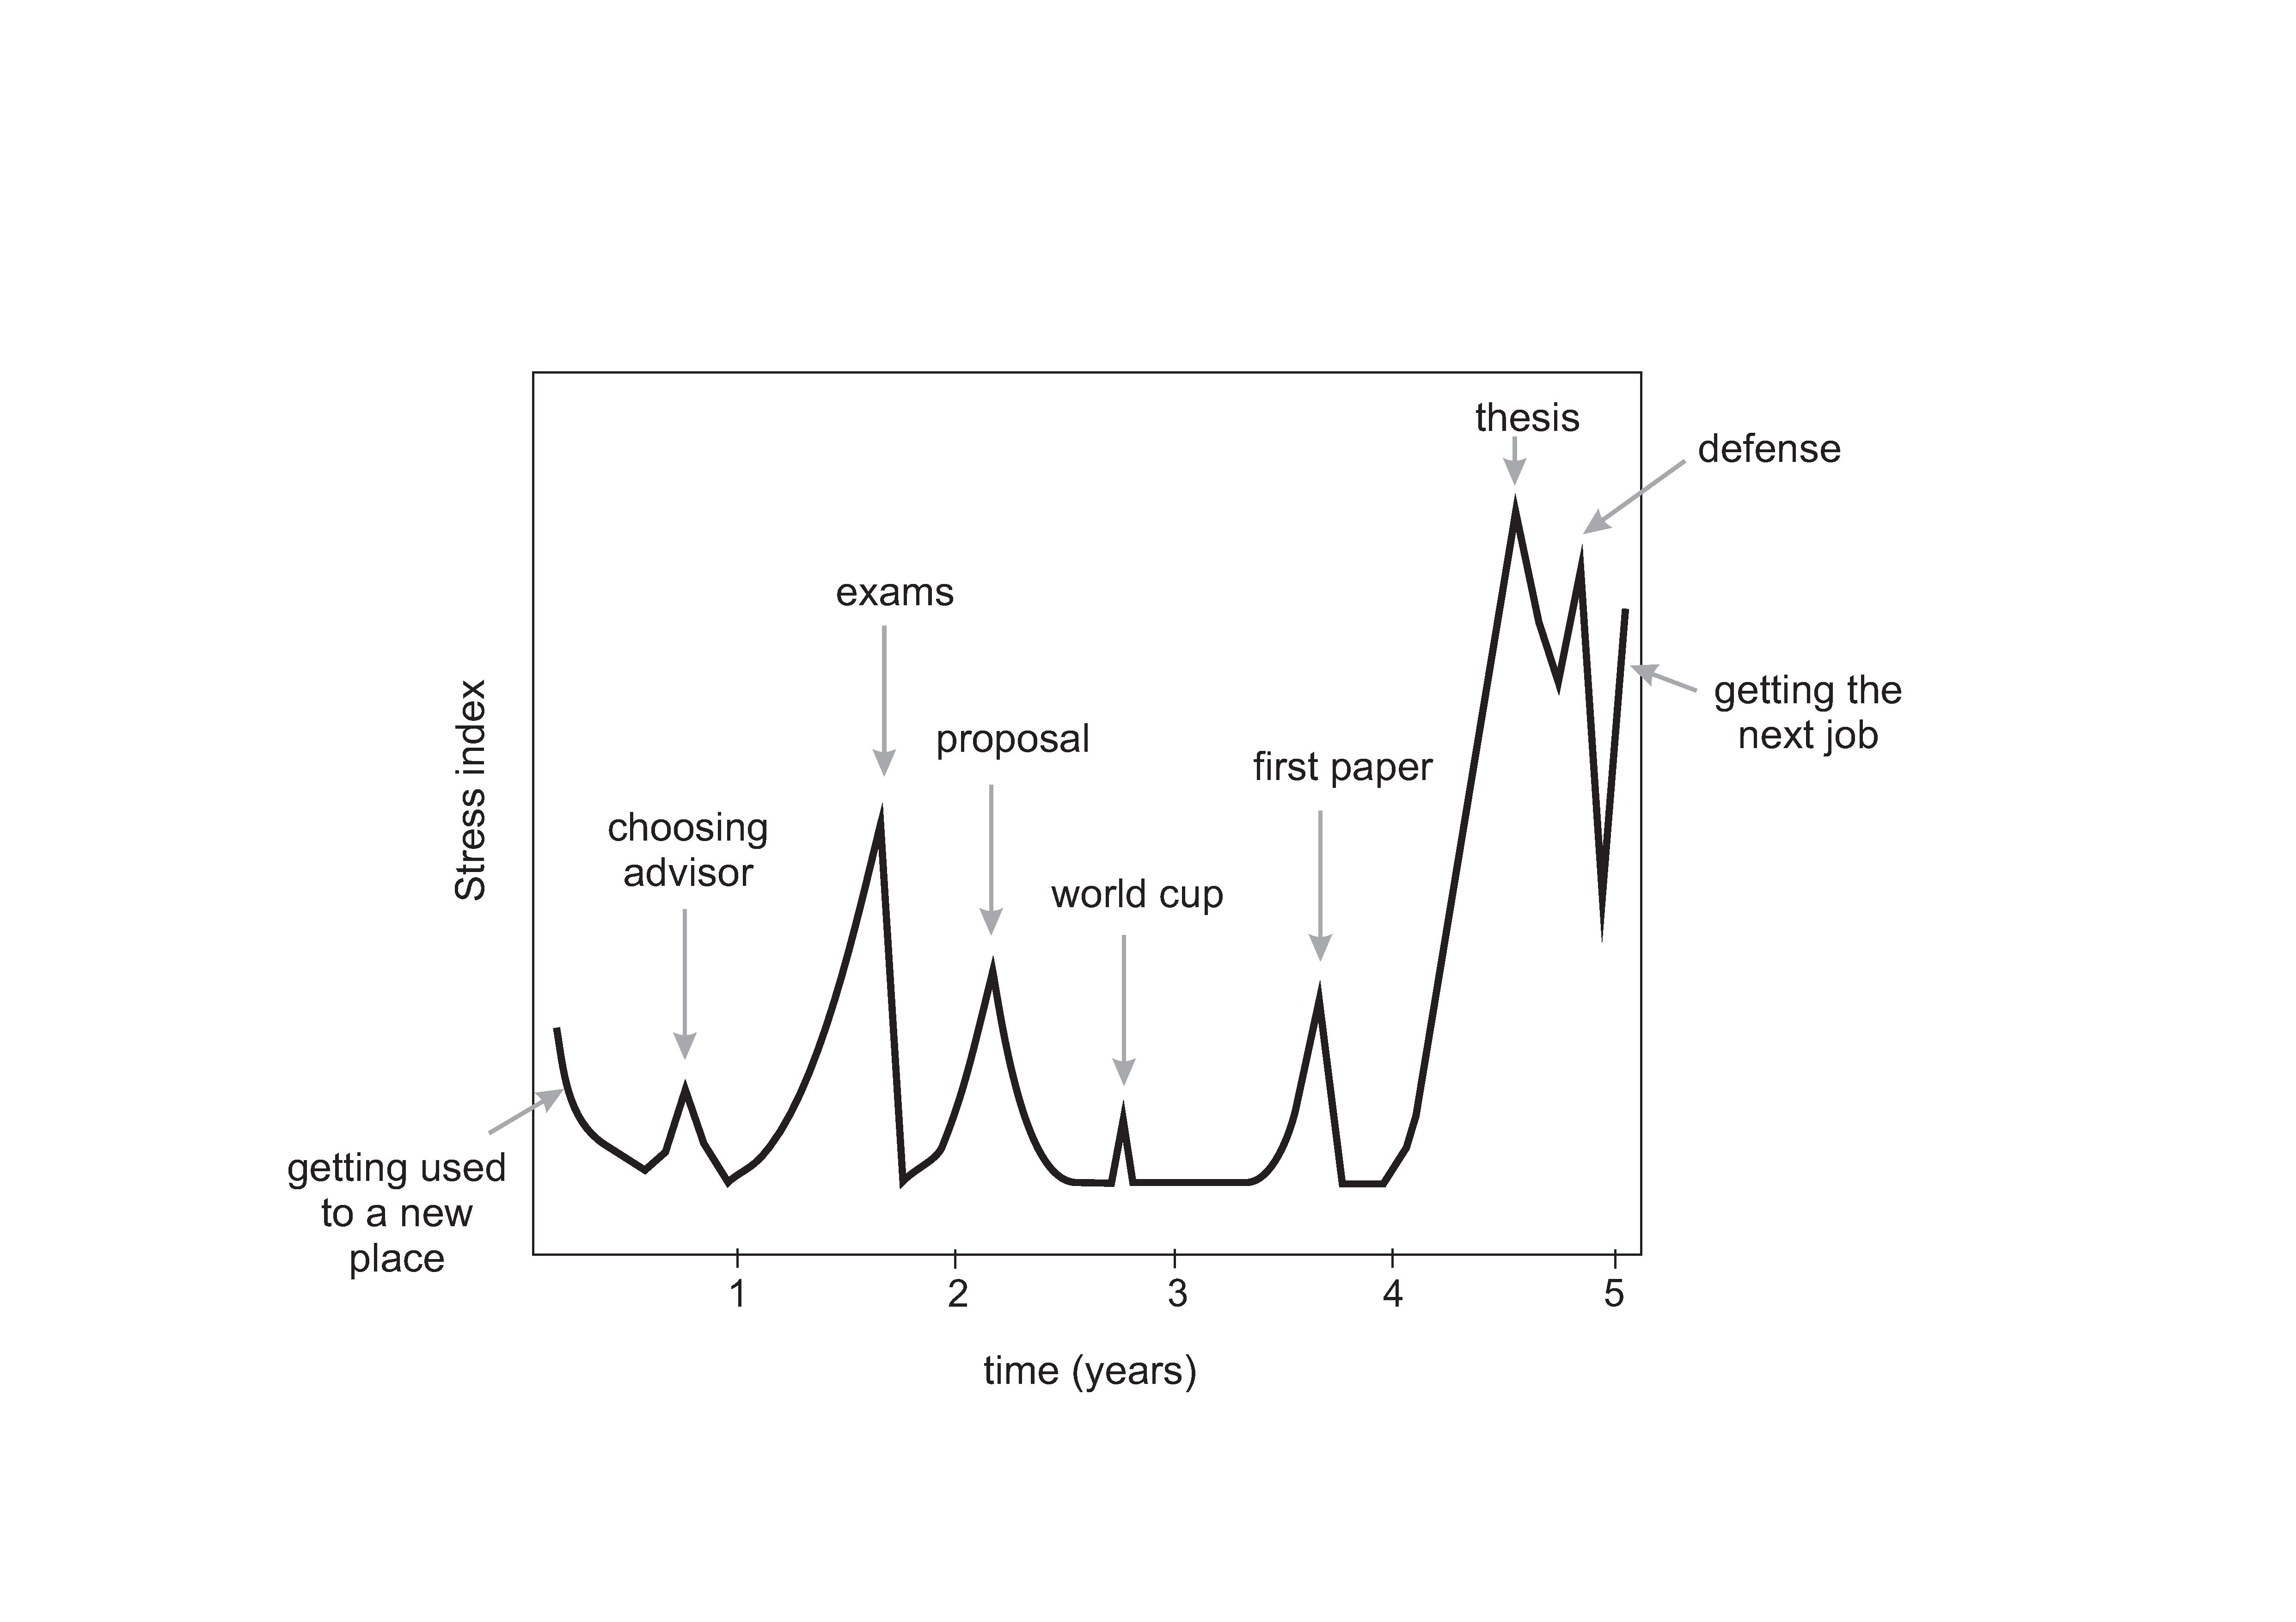
\includegraphics[width=.85\textwidth]{Fig_stress_curve_PhD.pdf}
\caption{The Graduate School stress curve\index{stress curve} by Edwin P.\@ Gerber\index{Gerber} (from a talk on how to survive grad school).} \label{Fig:stress_curve_PhD}
\end{center}
\end{figure*}

A typical academic career looks like this (see also Fig.\@~\ref{Fig:stress_curve_PhD}):

\begin{enumerate}
  \item First, three articles published in international peer-reviewed journals
  \item PhD promotion
  \item Post-doctoral projects (the next 10 important publications)
  \item Organize research conferences or collaborative projects (e.g.\@ editing books)
  \item Permanent position or research tenure
  \item Popularize developments in your field in the media
  \item Initiate (get funding for) your own projects and educational programs, and hire new PhD students and post-docs
  \item Become a senior researcher / professor.
\end{enumerate}

\emph{Initiation} i.e.\@ getting your first publication in a peer-reviewed journal is not a straightforward process and success is not guaranteed. Even if you were an excellent student at university, there's no guarantee that you will easily get published. There are some major misconceptions that need to be clarified:

\begin{itemize}
  \item Your supervisors will not take responsibility if your paper is rejected --- the responsibility will be entirely yours. Once you become a senior researcher or a professor you will discover how stressful it would be to take responsibility for everything your students produce (there is simply not enough time to go through all the material in detail).
  \item Likewise, many supervisors do not have time to read every text you write in detail and filter it according to the steps described in section~\ref{sec:filtering} (page~\pageref{sec:filtering}). Do not think that if your supervisor has no specific comments, your paper is okay and ready to publish. It probably isn't. You should read section~\ref{sec:filtering}, and go through the checklists listed there to minimize the chances of rejection.
  \item Journal editors are not part of your PhD committee and they are not interested in any arrangements you may have with your supervisors. The papers you intend to submit must be stand-alone documents that target the readers of the journal. After you publish a paper, you can make some minor modifications and adjust it so that it links more closely to your PhD thesis. Such adjusted papers can be published as \emph{``Based on$\ldots$ ''}.
  \item Journals will not fit in with your work tempo or project plans. Your paper can easily be delayed (even unintentionally), so make sure you submit papers to journals                              in the first half of your PhD study or at least 18 months before the planned defense.
  \item PhD students are \emph{at the bottom of the food chain} in the academic kingdom. Appreciate your supervisors and always be very professional (organized) when sending documents and undertaking work-related tasks.
\end{itemize}

\citet[p.67--68]{Creedy2008research} thinks that the worst things a PhD student can do when communicating with supervisors are (paraphrased):

\begin{itemize}
  \item \emph{Be unwilling to make suggested changes and/or carry out extensive revisions to drafts}
  \item \emph{Immediately claim that the supervisor is wrong about something}
  \item \emph{Send piles of computer output and expect the supervisor to sieve through all the detail}
  \item \emph{Send scrappy or highly provisional pieces of work and then expect extensive feedback}
  \item \emph{Ignore or treat lightly suggestions by supervisors}
  \item \emph{Ask to borrow books}.
\end{itemize}

In conclusion, if you're well organized, becoming a PhD is not as hard as it may seem. \citet[p.329]{Bloomfield2008} make a number of suggestions on how to get organized:

\begin{itemize}
  \item \emph{Set up a workspace with good working conditions}
  \item \emph{Follow an outline}, to ensure the most logical arrangement of topics
  \item \emph{Don't worry about getting all the wording right in the first draft}
  \item \emph{Start with writing things that are easiest} (methods and materials)
  \item \emph{Print out drafts and reread them after a break} (critically evaluate yourself)
  \item \emph{Make back-ups!}
\end{itemize}

 \citet{Weinberg2003Nature} suggested four golden rules for PhD students at the start of their careers:

\begin{enumerate}
  \item \emph{Don't be too anxious about a lack of background knowledge (no one knows everything, and you don't need to!)}.
  \item \emph{Go for the messy (unsolved problems$\ldots$ mysteries) --- that's where the action is}.
  \item \emph{Forgive yourself for wasting time. Unsuccessful experiments and dead-ends are quite normal}.
  \item \emph{Learn something about the history of science. Take a broad-brush approach}\footnote{Consider, for example, reading Carl Sagan's \emph{``Cosmos''} and/or Bill Bryson's \emph{``A Short History of Nearly Everything''}.}.
\end{enumerate}

You should have the guts to take risks. Learn how to swim in rough waters. Experimenting is OK if you are a PhD student, even if you find you need to flush some of your hard work and start again. \par

When you are presenting your work at an international conference you might get a chance to impress people with your presentation skills and slides. Scientific publication has to achieve the same result without all the bells and whistles. As we have emphasized several times in this book, the best way to convince an audience of your credibility is to produce a scientific publication of the highest quality. Researchers are now also experimenting with different ways to enhance the impact of their work by using, for example \textsf{pubcasts} --- short visual explanations of your research\footnote{See for example \url{http://www.scivee.tv} --- a channel for drawing attention to your research results through video presentations linked to your paper. All you need is a WebCam.}. Maybe this will help you express your ideas clearly and convince your colleagues?\par

Finally, the key to success with a PhD study probably lies in getting professional help from your co-authors, i.e.\@ your supervisors. If we were to put all of the ingredients needed for a successful PhD in order of importance, it would look something like this (the percentages in brackets indicate estimated weighting):

\begin{itemize}
  \item At least two supervisors who have the right advice at the right time and you can sit in their office and talk with them whenever necessary (50\%)
  \item Top laboratory and IT equipment, including software (20\%)
  \item Access to digital and hard copy libraries (15\%)
  \item Specialized training in academic writing, research skills, advanced statistical analysis and document preparation (10\%)
  \item Participation in international conferences and workshops (5\%).
\end{itemize}

About 50\% of a successful PhD thesis is down to having good supervisors, who are usually co-authors of your articles \citep{Creedy2008research}. And this typically does not cost much. If you prepare a solid draft or concept paper, then there's a better chance that you will be able to attract influential researchers and get them on board. Researchers are best rewarded by publications. If your supervisors or external colleagues recognize the potential in your paper, they will want to get involved. So, as with love, money can't buy you a PhD. Or to quote the Naked Chef: \emph{``I am not a doctor. I'm a chef. I do not have expensive equipment or medicine. I use information, education.''}\footnote{\url{http://www.ted.com/talks/jamie_oliver.html}} You too can prepare an excellent meal with a low budget.\par


\newpage

\section*{Recommended reading}

\noindent \textbf{On Free and Open Source Software manuals}:\index{Open Source Software}

\begin{itemize}
\renewcommand{\labelitemi}{$\bigstar$}
  \item Ayers, Ph., Matthews, C., Yates, B., 2008. \textbf{How Wikipedia Works}. No Starch Press, 536~p.
  \item Chambers, J.M. 2008. \textbf{Software for data analysis: programming with R}. Springer, 231~p.
  \item Kabacoff, R.I., 2011. \textbf{R in Action: Data analysis and graphics with R}. Manning publications, 470~p.\index{statistics!R book}
  \item Mittelbach, F., Goossens, M., Braams, J., Carlisle, D., and Rowley, C. 2004. \textbf{The \LaTeX Companion}, 2nd edition, Addison-Wesley Professional, 1120~p.
  \item Gay, J. (edt) 2002. \textbf{Free Software, Free Society: Selected Essays of Richard M.\@ Stallman}. GNU project, 226~p.
\end{itemize}

\bigskip
\noindent \textbf{On graphic design and scientific visualization}:

\begin{itemize}
\renewcommand{\labelitemi}{$\bigstar$}
  \item Goossens, M., Mittelbach, F., Rahtz, S., Roegel, R., and Voss, H. 2007. \textbf{The \LaTeX Graphics Companion}, 2nd edition, Addison-Wesley Professional, 976~p.
  \item Tufte, E.R., 1992. \textbf{The Visual Display of Quantitative Information}. 2nd Edition, Graphics Press, 197~p.
  \item Sarkar, D., 2008. \textbf{Lattice: {M}ultivariate Data Visualization with {R}}. Springer, Use R series, New York.
\end{itemize}

\bigskip
\noindent \textbf{On writing (and finishing) a PhD thesis}:

\begin{itemize}
\renewcommand{\labelitemi}{$\bigstar$}
  \item Creedy, J. 2008. \textbf{Research without tears: from the first ideas to published output}. Edward Elgar Pub., 118~p.
  \item Dupre, L. 1998. \textbf{BUGS in Writing}, Revised Edition: A Guide to Debugging Your Prose. 2nd ed., Addison-Wesley Professional, 704~p.
  \item Turabian, K.L. 2007. \textbf{A Manual for Writers of Research Papers, Theses, and Dissertations}. 7th ed., University of Chicago Press, Chicago, p.~436.
\end{itemize}

% \end{pagewiselinenumbers}


\backmatter%%%%%%%%%%%%%%%%%%%%%%%%%%%%%%%%%%%%%%%%%%%%%%%%%%%%%%%



\Extrachap{Appendix}

% Rules of thumb for writing research articles
% first version on 07.2002.
% Adjusted and modified for the purpose of "The unofficial guide for authors"
% \cleardoublepage
% \pagestyle{plain}

\cleardoublepage

\begin{flushright}
   \includegraphics[width=.8\marginparwidth]{sciwri2/ball01.pdf}
    \vspace{-10pt}
\end{flushright}

\begin{center}
\LARGE\textbf{Rules of thumb for \\ writing research articles}
\end{center}

\bigskip

\begin{center}
\begin{minipage}[c]{.85\textwidth}
\centering
     \renewcommand{\footnoterule}{}
     \setcounter{mpfootnote}{0}%
     \renewcommand{\thempfootnote}{\alph{mpfootnote}}%
    Tomislav Hengl\footnote{ISRIC --- World Soil Information, PO Box 363, 6700 AJ Wageningen} \& Michael Gould\footnote{Michael Gould Associates BV, Apeldoornseweg 21, NL-6814 BG Arnhem}
\end{minipage}
\end{center}

\bigskip

\noindent\rule{\textwidth}{.5pt}
\begin{wrapfigure}{o}{1.2\marginparwidth}
\centering
 \vspace{-10pt}
\includegraphics[width=1.2\marginparwidth]{sciwri2/ball02.pdf}
 \vspace{-20pt}
\end{wrapfigure}
\noindent\textbf{\emph{Abstract}---This paper lists `rules of thumb' for writing research articles (RA) and getting them published. These were discussed during a scientific writing course organized for ITC PhD students by Cressie Communication Services. Important aspects of the macro and sub-structure of a paper were explored in group discussions. The (meso)structure and functions of different sections of RAs are described. The results of previous investigations and interviews among journal editors were used to identify what makes a good RA.
It was concluded that clear, logical, coherent, balanced and well-structured writing gets papers published and read. Some important rules of the thumb were: \emph{Adjust your writing to the audience and purpose}, \emph{Avoid redundancy and unnecessary explanations} and \emph{Write like you speak and then revise}. These rules can help inexperienced writers present their work in a more effective way.}\par
\noindent\rule{\textwidth}{.5pt}

\begin{flushleft}
\emph{Key words}: research article, writing, rules of thumb, structure,
\end{flushleft}

% \begin{multicols}{2}

\section*{Introduction}

\begin{wrapfigure}{i}{.9\marginparwidth}
%\centering
 \vspace{-20pt}
\includegraphics[width=.9\marginparwidth]{sciwri2/ball04.pdf}
 \vspace{-20pt}
\end{wrapfigure}
A scientific or research article or paper is a technical (or essayistic?) document that describes a significant experimental, theoretical or observational extension of current knowledge, or advances the practical application of known principles \citep{oConnor1975writing}. It is important to emphasize the fact that a research article (further referred as RA) should report on research findings that are not only sound (valid) and previously unpublished (original), but also add some new understanding, observation, proofs, i.e.\@ potentially important information \citep{gordon1983running}. \par

Unlike a novel, newspaper article or an essay, an RA has a fixed, predefined structure and style, which is by international consensus known as \emph{Introduction-Methods-Results-Discussion} or IMRaD. However, an RA is not only a technically rigid document, but also a subjective intellectual product that unavoidably reflects personal opinions and beliefs. Therefore, it requires skill both in structuring and formulating concepts and findings. These skills are acquired through experience, but can also be taught.\par

\begin{wrapfigure}{o}{.9\marginparwidth}
%\centering
\vspace{-20pt}
\includegraphics[width=.9\marginparwidth]{sciwri2/ball05.pdf}
\vspace{-20pt}
\end{wrapfigure}
There are many books on general guidelines for scientists wishing to write RAs and survive the review process \citep{trelease1969write,day2006write,germano2008getting}. These days, many scientific societies publish quite detailed style manuals to help both authors and publishers; see for example the CBE's Style Manual (\citeyear{cbe1994scientific}) or the ACA-CSA-SSSA Manual (\citeyear{ASA-CSA-SSSA1998}). In this paper, the conventions for writing an RA are described in the terms of the macro, meso and micro-elements of the paper.\par

\begin{wrapfigure}{i}{\marginparwidth}
%\centering
\vspace{-20pt}
\includegraphics[width=\marginparwidth]{sciwri2/ball07.pdf}
\vspace{-20pt}
\end{wrapfigure}
Various authors have investigated the principles of creating a good title, writing a good abstract or introduction \citep{McPhee2001,swales2004academic}. Some go to the level of the micro-structure of the RA (sentences), providing guidelines for structure and style \citep{Gopen1990,turk1989effective,Kirkman2004S}.\par

However, writing an RA is a bit like climbing a \emph{monkey-puzzle tree}, especially if you are a non-native English speaker (further referred to as L2). \marginpar{\includegraphics[width=.9\marginparwidth]{sciwri2/ball06.pdf}} What makes a good paper and can we offer guidelines to young researchers?\par

\begin{wrapfigure}{i}{\marginparwidth}
%\centering
\vspace{-20pt}
\includegraphics[width=\marginparwidth]{sciwri2/ball09.pdf}
\vspace{-20pt}
\end{wrapfigure}
With this motivation, we tried to formulate some rules of thumb for writing (and publishing) RAs. These were gathered during discussions in the course \emph{``Scientific writing for non-native English speakers''}, but they also reflect our personal experience of scientific writing. \marginpar{\includegraphics[width=.9\marginparwidth]{sciwri2/ball08.pdf}}
The idea behind this paper was to summarize the main conclusions from these discussions in an easy-to-read format. \par

Note that we do not focus on correctness. Rather, we try to show how authors would be more/less likely to write in a particular way in a specific context. The need for unambiguous clear rules, rather than fuzzy preferences, is probably culturally determined \citep{hofstede2005cultures}. Fortunately, the structure of scientific writing is well-defined and we can also indicate what is effective style (in terms of readability).\par


\section*{Methods and materials}

The Scientific writing course, organized annually for ITC PhD students, was held between March 8 and April 26 in 2002. There were nine students, who followed five full-day classes. There was enough time to do homework --- mainly rewriting assignments in between classes. The classes were organized in such a way that the participants worked in groups or individually and discussed the most important issues, first among themselves and then with the whole group. \par

\begin{wrapfigure}{i}{\marginparwidth}
%\centering
\vspace{-20pt}
\includegraphics[width=\marginparwidth]{sciwri2/ball11.pdf}
\vspace{-20pt}
\end{wrapfigure}
The following topics were discussed in detail (in chronological order): the standard structure or elements of an RA, macro, meso and micro levels of an RA, general problems with readability and communication, the functions and content of the Introduction, Methods, Results and Discussion sections, writing successful abstracts and tips for submitting an RA for publication in a journal. \marginpar{\includegraphics[width=.9\marginparwidth]{sciwri2/ball10.pdf}} The participants were from eight countries (L2) and four continents, which provided a good basis for discussing cultural-academic differences \citep{Prince1999}. \par

\begin{wrapfigure}{o}{\marginparwidth}
%\centering
\vspace{-20pt}
\includegraphics[width=\marginparwidth]{sciwri2/ball13.pdf}
\vspace{-20pt}
\end{wrapfigure}
The material and facilities were organized by Ian Cressie \citeyear{Cressie2002}\index{Cressie}, while most of the classes were led by Michael Gould, documentation consultant and advisory editor. The participants generated some graphs and flow diagrams manually (Fig.\@~\ref{Fig:ITCgroup}), which we then modified and transferred to a manuscript form. \par

\begin{figure*}[!htb]
\begin{center}
\includegraphics[width=.8\textwidth]{sciwri2/Fig_discussion.jpg}
\caption{Photo from the Scientific writing class at ITC. Discussion about the \emph{``Discussion''} section.} \label{Fig:ITCgroup}
\end{center}
\end{figure*}

\begin{wrapfigure}{i}{.9\marginparwidth}
%\centering
\vspace{-20pt}
\includegraphics[width=.9\marginparwidth]{sciwri2/ball14.pdf}
\vspace{-20pt}
\end{wrapfigure}
The basic concept of the course is that the students should learn from real examples and their own mistakes. In most cases, participants were analyzing and correcting each other's work. In other cases, participants were making comments on examples prepared by Ian Cressie. A typical exercise was, for example: a short RA is given to students who have to write an abstract, respecting the appropriate conventions. \par

Most of the rules mentioned in this article were agreed by the majority of participants. \marginpar{\includegraphics[width=\marginparwidth]{sciwri2/ball12.pdf}}We have also used the results of previous investigations and inquiries by journal editors to support general conclusions. Nevertheless, some of the statements and principles reflect personal views and opinions and should not be confused with the cited literature. The tips given here apply mainly to application-based sciences and RAs intended for publication in such journals.\par


\section*{Results}
\subsection*{RA structure and style}

\begin{wrapfigure}{o}{.9\marginparwidth}
%\centering
\vspace{-20pt}
\includegraphics[width=.9\marginparwidth]{sciwri2/ball15.pdf}
\vspace{-20pt}
\end{wrapfigure}

A RA was first divided into a number of sections (futher referred to as RAS) and elements (RAE). The participants agreed that the main article sections that are required in any modern journal are, in this order: Title, Authors, Abstract, Introduction (I), Methodology (M), Results (R), Discussion (D) and Conclusions and References. These are the core of an RA. Additional listed RAS's were: Author-paper documentation, Keywords, Acknowledgements, Abbreviations and Appendices. The RAEs listed were: tables, figures (plus graphs, maps, diagrams, and sketches), equations, citations and footnotes and comments. The RAEs can come in different places in the RA. However, tables and figures are more usual in the Results section and equations and citations in the Methods section and Introduction. All of these RAS's and RAEs have their function and required style and should form a coherent whole. The functions of the main RAS's are described in Table~\ref{Tbl:functions}.\par

{\small
\begin{sidewaystable}[!hp] \addtolength{\tabcolsep}{4pt}
\centering \caption{Research Article Sections (RAS), main functions, preferred style and related rules of thumb.}\label{Tbl:functions}
\begin{tabular}{m{.08\textwidth}m{.25\textwidth}m{.25\textwidth}m{.35\textwidth}}
\toprule
RAS & Main functions & Preferred style & Rules of thumb \\
\midrule
Title & \begin{itemize}  \item Expresses the content and main discoveries \item Attracts the reader's attention \end{itemize} & \begin{itemize} \item Short and simple words (7-10) \item Purposive (targets a specific audience) \end{itemize} & \begin{itemize} \item Avoid complex grammar; make it catchy! \item Avoid redundancy (``\emph{An investigation of... }'', ``\emph{The analysis of... }'', ``\emph{Effect of... }'', ``\emph{Influence of... }'', ``\emph{New method...}'') \end{itemize} \\
Abstract & \begin{itemize} \item Reflects the main `story' of the RA \item Calls attention but avoids extra explanations \end{itemize} & \begin{itemize} \item Past (perfect) tense and passive voice \item Short concise sentences \item No citations, tables, equations etc. \end{itemize} & \begin{itemize} \item Avoid introducing the topic \item Explain: what was done, what was found and what are the main conclusions \item Provide summary `numbers' \end{itemize} \\
Introduction & \begin{itemize} \item Introduces the topic and defines the terminology \item Relates to existing research \item Establishes the focus of the paper and research objectives \end{itemize} & \begin{itemize} \item Present tense for referring to established knowledge and past tense for literature review \item Extensive overview of literature \end{itemize} & \begin{itemize} \item Use state-of-the-art references \item Follow logical moves \item Define your terminology to avoid confusion \item Establish an author's voice \end{itemize}  \\
Methodology & \begin{itemize} \item Provides enough detail for competent researchers to repeat the experiment \item Who, what, when, where, how and why? \end{itemize} & \begin{itemize} \item Past tense \item Correct and internationally recognized style and format (units, variables, materials etc) \end{itemize} & \begin{itemize} \item Mention everything you did that influenced the results; don't cover your traces (``\emph{some data was ignored}'') \item If a technique is widely known, refer to it by its name (don't re-explain it) \item Use the simple(st) examples to explain complex methodology \end{itemize} \\
\bottomrule
\end{tabular}
\end{sidewaystable}
}

{\small
\begin{sidewaystable}[!hp] \addtolength{\tabcolsep}{4pt}
\centering \caption{Research Article Sections (RAS), main functions, preferred style and related rules of thumb (continued).}\label{Tbl:functions2}
\begin{tabular}{m{.08\textwidth}m{.25\textwidth}m{.25\textwidth}m{.35\textwidth}}
\toprule
RAS & Main functions & Preferred style & Rules of thumb \\
\midrule
Results & \begin{itemize} \item Provides summary results in tables and graphs \item Compares different `treatments' \item Provides quantified proofs (statistical tests) \end{itemize} & \begin{itemize} \item Past tense \item Use tables and graphs and other illustrations \end{itemize} & \begin{itemize} \item Present summary data directly related to your research question and not all research results \item Call attention to the most significant findings \item Make a clear distinction between your work and that of others \end{itemize} \\
Conclusions and Discussion & \begin{itemize} \item Clearly answers research questions/objectives \item Explains discrepancies and unexpected findings \item States importance of discoveries and future implications \end{itemize} & \begin{itemize} \item Simple past and/or present tense (past tense when related to results) \item Allows scientific speculation (if relevant) \end{itemize} & \begin{itemize} \item Do not recapitulate results but make statements \item Make strong statements where they are justified (avoid ``\emph{It may be concluded... }'' style) \item Do not hide unexpected results --- they may be the most important ones \end{itemize} \\
References & \begin{itemize} \item Provide a list of related literature and sources of information \item Support the ideas in the paper \end{itemize} &
\begin{itemize} \item Depends on journal, but authors/editors, year and title must be included \end{itemize} &
\begin{itemize}
    \item Always cite the most accessible references
    \item Cite primary source rather than review papers
\end{itemize} \\
\bottomrule
\end{tabular}
\end{sidewaystable}
}

\begin{wrapfigure}{i}{.9\marginparwidth}
%\centering
\vspace{-20pt}
\includegraphics[width=.9\marginparwidth]{sciwri2/ball17.pdf}
\vspace{-20pt}
\end{wrapfigure}

The participants agreed that some RAs, even with good data and interesting results, will be rejected if the style and format of the paper are not tailored to the needs of a particular audience. This confirms the results of \citet[Fig.1]{Gosden1992} who asked over 100 journal editors what they thought were the most important issues for non-English authors who want to get published. These were, in order of priority:

\begin{enumerate}
    \item Clear, logical linking of sentences
    \item Coherent development of the topic (old before new information)
    \item Use of grammatically correct sentences
    \item An ability to make effective claims at the right level
    \item Clear organization of sections of a paper, and
    \item Placing their work in a wider context (especially relevant for authors in developing countries).
\end{enumerate}

The misplacement of old and new information is not just a problem for non-native speakers, it is also the No.~1 problem in American professional writing \citep{Gopen1990,germano2008getting}. The participants analyzed a flawed paper by an unknown author and decided, after some discussion, that they would reject the publication.


\subsection*{RA sub-structure}


\begin{wrapfigure}{i}{.9\marginparwidth}
%\centering
\vspace{-20pt}
\includegraphics[width=.9\marginparwidth]{sciwri2/ball16.pdf}
\vspace{-20pt}
\end{wrapfigure}

The participants also discovered that all RAS's can be separated into subsections using clear signposts, which can improve the way the argument is built up in an RA. The subsections we identified were: research topic and definitions, research objectives (questions), methodological techniques, experimental set-up, context of the study (e.g.\@ study area), main discoveries (analyzed data), answers to research questions, explanation of the conclusions and further research and implications. The main RAS's are listed in a flow chart, showing the main relationships between the different sections (Fig.\@~\ref{Fig:paper}). Fig.\@~\ref{Fig:introdisc} shows the substructure of the Introduction and Discussion --- the most important RAS's.\par\index{introduction}

\begin{figure*}[htb]
\begin{center}
\includegraphics[width=.9\textwidth]{Fig_RA_elem.pdf}
\caption{Flow diagram: research article sections\index{sections}\index{research article} (shaded) and subsections, and their main relations.} \label{Fig:paper}
\end{center}
\end{figure*}

\begin{figure*}[htb]
\begin{center}
\includegraphics[width=.65\textwidth]{Fig_RAS.pdf}
\caption{Flow diagram: logical framework for the Introduction and Discussion, as agreed by most of the participants.\index{discussion}} \label{Fig:introdisc}
\end{center}
\end{figure*}

\section*{Discussion and Conclusions}

\begin{wrapfigure}{o}{.9\marginparwidth}
%\centering
\vspace{-20pt}
\includegraphics[width=.9\marginparwidth]{sciwri2/ball18.pdf}
\vspace{-20pt}
\end{wrapfigure}

What is the purpose of an RA and what makes it a good one, and who decides that it is a good RA? Are there rules for easier writing? If the main function of an RA is to transfer new knowledge on a research topic, then a good paper is one that is clear, coherent, focused, well argued and uses language that does not have any ambiguity. However, it is not only the message that is important. The RA must have a well-defined structure and serve as a kind of cook book, so that others can reproduce and repeat the experiments described in it. There are some rules that can make the writing and publishing of RAs easier. Here, we summarize some which should always be kept in mind by an inexperienced researcher (Table~\ref{Tbl:golden}). We put all of these together to make a list of some 40 logical steps, which can be found at the end of this article.\par

% \renewcommand{\baselinestretch}{1.5}
{\small
\begin{table*}
\begin{center}
  \caption{Selected golden rules\index{golden rules} for easier publishing.}\label{Tbl:golden}
 \vspace{5pt}
\begin{tabular}{m{.4\textwidth}m{.55\textwidth}}
\toprule
\emph{Rule} & \emph{Explanation} \\
\midrule
Take a reader's view & Write for your audience not for yourself. \\
\midrule
Tell a story & Direct your RA but keep a clear focus in the paper and present only results that relate to it. \\
\midrule
Be yourself & Write like you speak and then revise and polish. \\
\midrule
Make it simple & Use simple(st) examples to explain complex methodology. \\
\midrule
Make it concrete & Use concrete words and strong verbs, avoid noun clusters (more than three words), abstract and ambiguous words. \\
\midrule
Make it short & Avoid redundancy, repetition and over-explanation of familiar techniques and terminology. \\
\midrule
Take responsibility & Make a clear distinction between your work and that of others. \\
\midrule
Make strong statements & \emph{``We concluded$\ldots$ ''} instead of \emph{``It may be concluded$\ldots$ ''} \\
\midrule
Emphasize & Learn to use little words in a big way. \\
\midrule
Be self-critical & Consider the uncertainty of conclusions and their implications and acknowledge the work of others. \\
\midrule
Never stop editing & The key to writing well is extensive editing.\\
\bottomrule
 \end{tabular}
\end{center}
\end{table*}}


\begin{wrapfigure}{i}{\marginparwidth}
%\centering
\vspace{-20pt}
\includegraphics[width=\marginparwidth]{sciwri2/ball19.pdf}
\vspace{-20pt}
\end{wrapfigure}

Although it was assumed in the past that \emph{`thicker'} articles with a wider range of vocabulary are preferable, most editors (and readers) prefer simple, clear and coherent writing (KISS --- Keep It Short and Simple)\index{KISS}, rather than a fancy or complex, pseudo-scientific style. \citet{Funkhouser1971} showed that information gain is especially enhanced by the \emph{use of examples}, i.e.\@ it helps a lot to use parallels from everyday life, historical references, etc. Some sections, such as the Introduction and Discussion, must intrigue readers, and capture their interest. For example, an interesting title can catch readers' attention and will be easily remembered (e.g.: T.Y.\@ Li and J.\@ Yorke named their famous paper on chaos: ``\emph{The period three means chaos}''). Some sections simply require more skill and are more important. \par

It is estimated that of all the published journal RAs in the world, less than 5\% are read in detail. However, more than 50\% of abstracts are read and so the quality of an abstract is much more important. Therefore, the abstract should present the `story' of the RA in miniature and should make sense stand-alone.\par

The sub-structure of an Introduction was first described by \citet{swales1981aspects} with his ``\emph{four moves}''\index{logical moves}. These later on become three, the so-called CaRS (Create-A-Research-Space) model \index{Create-A-Research-Space}, which are: establish a research \emph{territory}, establish a research \emph{niche}, and then occupy the niche \citep{swales2004academic}. The participants in the course concluded that especially the meso-structure of the Introduction and Discussion should follow a logical flow of \emph{`moves'}, similar to playing chess (Fig.\@~\ref{Fig:paper} \& \ref{Fig:introdisc}).

The more structured and precise a paper is, the greater the chance that it will get published. Each of the RA elements has to fulfil its function in order to achieve this goal. \par

\begin{wrapfigure}{i}{.9\marginparwidth}
%\centering
\vspace{-20pt}
\includegraphics[width=.9\marginparwidth]{sciwri2/ball20.pdf}
\vspace{-20pt}
\end{wrapfigure}

The importance of following a logical structure is nicely illustrated by \citet{Gopen1990}:\index{signposts} ``\emph{People need signposts to understand what you're communicating. First establish the context based on what they know. Then move towards the new facts you want to convey. Beginning with exciting new information and ending with something we already know leaves us disappointed and spoils the flow}.''\par

However, this is not the whole story. An RA must target a specific audience/journal, has to be novel and of high interest. Finally, one thing should be uppermost in researchers' minds: a good article is not only an article that has been published in a top journal --- it is the reaction it generates that makes the difference. \par

\begin{wrapfigure}{o}{\marginparwidth}
%\centering
\vspace{-20pt}
\includegraphics[width=\marginparwidth]{sciwri2/ball22.pdf}
\vspace{-20pt}
\end{wrapfigure}

Therefore, a good article is not just one that is well written. A good article is one that is read and cited. In some cases, even a good paper will be rejected. Unfortunately, sometimes the reasons for this can be subjective (perhaps in around a third of all cases). Editors are often biased, they prefer one or another approach, academic level, gender\ldots nation. These problems and issues such as fraud, plagiarism and ethics are not discussed here, but they certainly are important.\par

Searching, inputting and formatting references has been much improved lately with the help of so-called \emph{``information management tools''} (web applications, on-line libraries, reference management tools, etc.). In addition, the role of companies involved in sorting and filtering, such as the Thompson's Web of Knowledge, will become more important. \par

\begin{wrapfigure}{i}{.9\marginparwidth}
%\centering
\vspace{-20pt}
\includegraphics[width=.9\marginparwidth]{sciwri2/ball23.pdf}
\vspace{-20pt}
\end{wrapfigure}

In the future, we can expect more structured guidelines for writing an RA (perhaps even templates?). The RA will also probably support multimedia (animations, sound recordings), which will improve communication between authors and readers/users. These innovations will inevitably require some new rules of thumb.\par

%\end{multicols}{2}

\bigskip

\emph{We would like to thank Ian Cressie for arranging the courses at ITC, which are of great importance to L2 PhD students. We also thank former ITC PhD student Jose L.C.\@ Santos and Dr.\@ David G.\@ Rossiter for reading the text and making their valuable suggestions.}

\begin{figure*}[!htp]
\begin{center}
\includegraphics[width=1.1\textwidth]{sciwri2/Fig_40steps.pdf}
\caption{The 40 steps you need to follow to write an RA.} \label{Fig:40steps}
\end{center}
\end{figure*}


\Extrachap{References}

\bibliographystyle{phppcf}
% \twocolumn
{\small \bibliography{UG4A_book} }


\printindex


\end{document}
